\documentclass[12pt]{book}[twoside,openright]

%\documentclass{book}[twoside,openright]
%\usepackage[fontsize=20pt]{scrextend}

%\usepackage{fourier}
%\usepackage[T1]{fontenc}

\usepackage{thesis_pdf}

%\setromanfont{ppl}
%\newcommand*{\myfont}{\fontfamily{qbf}\selectfont}
%\DeclareTextFontCommand{\textmyfont}{\myfont}

%\newcommand{\lParen}{\text{\textmyfont{\char"2685}}}

\newcommand{\starp}{\scalebox{0.8}{\(\star\)}} 


\usepackage[backend=biber,
style=alphabetic,maxbibnames=99]{biblatex}
\bibliography{references}

\newenvironment{contex}{
   \addtocounter{ex}{-1} \begin{ex}[continued]}{
   \end{ex}}

\setcounter{chapter}{-1}





\makeindex


\begin{document}
    \setlength\fboxsep{0pt}
    
    
{
%\sffamily 

\begin{titlepage}

{\Large Fennecs Swaddle}

{\tt \href{https://orcid.org/
0000-0002-2448-9512}{ORCID: 0000-0002-2448-9512}}

\vspace{2cm} 


\textbf{\semihuge\color{offblack}  Deformation quantisation and Airy structures}

\vspace{2cm} 



School of Mathematics and Statistics

The University of Melbourne

\today 
\vfill 

{\vspace{2cm}A thesis submitted for the degree of Doctor of Philosophy }



%\begin{flushright}
%
\includegraphics[scale=1.0]{logos/PRIMARY_A_Vertical_Housed_CMYK.eps}
%\end{flushright}


\end{titlepage}
}


    %\newpage \ \thispagestyle{empty} \newpage 
    
    
\thispagestyle{empty}

{
\color{offblack}\Large\bfseries Declaration}

\vspace{2em}

This thesis is an account of research undertaken between March 2018 and August 2022 at The School of Mathematics and Statistics, Faculty of Science, The University of Melbourne, Melbourne, Australia.

Except where acknowledged, the material presented in this thesis is, to the best of my knowledge, original and has not been submitted in whole or part for a degree in any university. 

The thesis is fewer than 100,000 words in length, exclusive of bibliographies, maps and tables.

\vfill

\begin{flushright}
\rule{14em}{0.6pt}\\
Michael Swaddle\\
\today
\end{flushright}
  
    \thispagestyle{empty}

{
\color{offblack}\Large\bfseries Acknowledgements}

\vspace{2em}


First, we would like to thank our supervisor Prof. Paul Norbury, for sharing his knowledge and many valuable insights. 

Also thank you to Dr. Wee Chaimanowong, and Dr. Mehdi Tavakol for many interesting mathematical discussions.

A huge thank you to Grant Kluber, for being a constant source of kindness, support and for listening to our problems. Thank you so much for all the random puzzles and fennecs.

Next, thanks to all my friends, particularly Harry and Alex for the core pandemic memories, helping us get through all the lockdowns with amusing content. Also Alex for all the Patricia coffees, lunch excursions, and general chaos.

Also a shout out to all the Weapon runners: Rocky, Duck, Slash, Popeye, Weapon, and the rest, especially for sharpening up so we could get the marathon and 5km bragging rights over Paul. 

We would also like to thank the University of Melbourne for giving us the opportunity to conduct this research.

Finally, we would like to thank our parents for supporting us throughout the entire journey.


\vfill

    %
\thispagestyle{empty}

{

%\sffamily
\color{offblack}\Large\bfseries Preface}

\vspace{2em} 

\vfill  
    %\newpage \ \thispagestyle{empty} 
    
    %\newpage     
    
    \setcounter{page}{1}
    \tableofcontents 
    
    
    
    \chapter{Preliminaries}
    \label{chapter:prelim}


    \section{Introduction and overview}
    

    Chapter (\ref{chapter:deformation}) starts with a review of deformation quantisation. We make the observation that what is termed a generator for a cyclic DQ module, or a \emph{wavefunction} in other literature, for example in \cite{ks_airy}, should be viewed from a sheaf theoretic perspective, as modules over a deformed sheaf of algebras. We also reprove an obstruction result for the existence of quantisation with greater clarity. This chapter is reproduced mostly from our own paper \cite{swaddledef}.
    
    Chapter (\ref{chapter:tate}) is a description of the topology required by Kontsevich and Soibelman to define Airy structures in infinite dimensions. In particular we describe the Tate space of differentials. Apart from an attempt at a clear exposition, we also incorporate details from our joint paper \cite{chaimanowong2020airy} proving some geometrical details. Chapter (\ref{chapter:infalg}) is an algebraic analog for the coordinate rings on Tate spaces. 
    
    Chapter (\ref{chapter:airy}) gives the definition of an Airy structure. Airy structures were originally defined by Kontsevich and Soibelman,  \cite{ks_airy}. Our contribution is an attempt at describing them from a more algebraic geometric perspective, and a graphical algorithm to compute terms in some resulting power series.
    
    Chapter (\ref{chapter:symplecticreduction}) explains a process known as symplectic reduction. In particular, we investigate the symplectic reduction of wavefunctions, which are defined in chapter (\ref{chapter:deformation}).
    
    Chapter (\ref{chapter:Atensor}) is based on our paper with Paul Norbury, Mehdki Tavakol and Wee Chaimanowong \cite{chaimanowong2020airy}. We mostly reproduce the contents of the paper, but it is appropriate here as it represents a coalescence of the previous chapters into an interesting result. 
    
    Previous work, \cite{chaimanowong2020airy, abcd, higherairy, eynard_orantin} studied various additional aspects of Airy structures. \cite{chaimanowong2020airy} was primarily concerned with aspects of symplectic reduction, while \cite{abcd} studies classifications of Airy structures. Following ideas from Kontsevich and Soibelman, the overall goal of this thesis is to fill in a missing link, and relate aspects of \emph{Airy structures} and \emph{topological recursion} using \emph{deformation quantisation}. The deformation quantisation aspect was not present in \cite{chaimanowong2020airy} and \cite{abcd}, and leads to interesting insight into the objects known as wavefunctions.

    
    
    \section{Eynard-Orantin Topological recursion}


    \emph{\hyperref[defn:tr]{Topological recursion}}, by Eynard and Orantin \cite{eynard_orantin}, is a recursive algorithm in two non-negative integers \((g,n)\), which produces a collection of symmetric, poly-differentials, \(\omega_{g,n}\). Many interesting invariants arising from problems in enumerative geometry and string theory can be computed by topological recursion, via different choices of the initial data given by \(\omega_{0,3}\) and \(\omega_{1,1}\). Topological recursion was first studied in the context of free energies of matrix models \cite{CEyHer}. The initial data can be encoded in an object called a \emph{\hyperref[defn:spectral_curve]{spectral curve}}.
    
    We give a slightly different definition of spectral curve
    to bridge the difference between the definition in \cite{eynard_orantin} and \cite{ks_airy}. Let \((X,\mathcal{O}_X) \) be a scheme over a field \( \mathbf{k}\) of characteristic zero, usually \( \mathbb{C}\).
    \begin{defn}[Weil divisor] A \emph{divisor} \(D\) on \(X\) is a formal \(\mathbb{Z}\)-linear combination 
    \[ D = \sum_j k_j Z_j,\]
    where \(Z_j\) is a codimension 1 subscheme, \(k_j \in \mathbb{Z}\).
    \end{defn}
    %If \(X\) is a Riemann surface, codimension 1 submanifolds are points.
    %Recall the space of K\"ahler (holomorphic) differentials is denoted \( \Omega_{\Sigma/\mathbb{C}}\). 
    %The de-Rahm complex is \( \Omega^n_{\Sigma/\mathbb{C}} = \bigwedge^n \Omega_{\Sigma/\mathbb{C}}\).
    
    %\begin{defn}[Symmetric bi-differential]
    %\end{defn}
    Now let \( (X,\mathcal{O}_X)\) be a complex algebraic surface. For any Weil divisor \(D\) there is an associated sub-sheaf \( \mathcal{O}_X(D)\), of the sheaf  of rational functions \(\mathcal{K}_X\) on \(X\). \( D\) is called \emph{Cartier} if \( \mathcal{O}_X(D)\) is an invertible sheaf. Let \( \mathcal{M}_X\) be the sheaf of meromorphic functions.
    

    
    \begin{defn}[Spectral curve]
    \label{defn:spectral_curve} 
    The tuple \( ( \Sigma, x,y,B)\) is called a \emph{spectral curve} where:
    
    
    \begin{itemize} 
    \item \( \Sigma \) is a Riemann surface.

    \item \(D_\Sigma \) is a Cartier divisor.
    
    \item \(x \in  \mathcal{O}_\Sigma(D_\Sigma)\) is a meromorphic function, such that \(dx \in  \Omega_{\Sigma}^1 (D_\Sigma)\) is algebraic, and zeros of \(dx\) are simple. Note \(D_\Sigma\) allows for arbitrary order poles at points.
    
    \item  \(y \in  \mathcal{M}_\Sigma\) is a meromorphic function regular at \(D_\Sigma \).

    \item  \( B \in H^0( \Sigma \times \Sigma, (\Omega_\Sigma^1 \boxtimes \Omega_\Sigma^1)(2 \triangle)) \) is a global symmetric bi-differential, \( \triangle = \mathrm{diag}(\Sigma \times \Sigma) \).
    \end{itemize}
    
    
    \end{defn}
    Later this data will be specified by a  \emph{foliation} on a symplectic surface \(X\). \( \Sigma\) becomes a curve in \(X\), \( \Sigma \rightarrow X\). The foliation defines a divisor \(D\), and then \(D_\Sigma = D \cap \Sigma\). 
    
    \begin{rem}
    \(x\) and \(y\) give a local and possibly global embedding of \(\Sigma \) into \( \mathbb{C}^2\).
    In the latter cases, this can be considered a subvariety generated by an ideal \( \langle P(x,y)\rangle\), in \( \mathbf{k}[x,y]\), where \(P(x,y)\) is a polynomial.
    \end{rem}
    
    
    
    %gives local (possibly global) embedding into \( \mathbb{C}^2\),
    
    % x,y local embedding in C^2
    %eynard oratin start with curve in C^2
    
    %Define the divisor \(R\) as the formal combination of order and zeroes of \(dx\).
    
    Consider a spectral curve \( (\Sigma,x,y,B)\).
    Define the divisor \(R\) as the simple zeros of \(dx\): 
    \[ R = \{ \alpha : d x(\alpha) = 0 \} \]
    Consider \( \alpha \in  R\), and \( U_{\alpha} \subset \Sigma\) be an open neighbourhood around \(\alpha\).
    %\begin{defn}[Galois involution] A \emph{Galois involution} is a locally defined map \(\sigma : U \rightarrow U\), such that \( x = x \cdot \sigma \).
    %\end{defn}
    %Recall in complex analysis, the residue of a complex function \(f\) along a closed curve \( \gamma\) is defined as \[\Res(f,\gamma) = \frac{1}{2 \pi i} \oint_\gamma f d z. \] 
    %\begin{defn}[Residue] The \emph{residue} is a linear functional, pairing a complex differential with a cycle:
    %\[ \Res : H^1(\Sigma,\mathbf{k}) \rightarrow H_1(\Sigma,\mathbb{Z}) \rightarrow \mathbf{k}.\]
    %\end{defn} 
    %The residue defines a symplectic form on the space of meromorphic differentials.
    %\begin{lem}[Symplectic form from residue]
    %\[ \omega(\psi,\eta) = \sum_{\alpha \in D_\Sigma } %\mathrm{Res}(f \eta, \alpha), \]
    %where locally \( d f = \psi\).
    %\end{lem}
    \begin{defn}[Local Galois involution]
    A \emph{local Galois involution} is a map defined locally around \(\alpha \in R\), and must satisfy \( x( \sigma_{\alpha}(p)) = x(p)\) for \( p \in U_{\alpha}\), \( \sigma_{\alpha}(\alpha) = \alpha \), \( \sigma_{\alpha}(p) \neq p\), for \(p \neq \alpha \in U_{\alpha}\).
    \end{defn}
    This definition uniquely determines \( \sigma_{\alpha}\).
    
    \begin{defn}[Recursion kernel]
    The \emph{recursion kernel} is a locally defined function \( K : U_{\alpha} \times U_{\alpha} \rightarrow \mathbb{C}\).
    \[ K(p_1, p)  = -\frac{1}{2} \ddfrac{\int_{\sigma_{\alpha}(p)}^{p} dw \, B(p_1,w)}{(y(p) - y(\sigma(p))) \, dx(p)}. \]
    \end{defn}
    Note the cancellation of the differentials.
    
    
    From the initial data of a spectral curve \((\Sigma, x,y,B)\) define two meromorphic differentials, \( \omega_{0,1}(p_1) = y(p_1) dx(p_1)\) and \( \omega_{0,2}(p_1, p_2) = B(p_1,p_2)\), and \(p\) is a local coordinate on \( \Sigma\).
    
    \begin{defn}[Topological recursion]\label{defn:tr} \emph{Topological recursion} is the collection of tensor products of meromorphic differentials \( \omega_{g,n} \in  H^0((\Sigma \setminus D_\Sigma)^n,(\Omega^1_\Sigma)^{\boxtimes n})\), which we call polydifferentials, defined by the quadratic recursive formula as follows:
    \begin{align*} 
    \omega_{g,n}(p_1, \dots p_n) =& \sum_{\alpha \in R } \Res_{z = \alpha}  K(p_1, p)     \Big( \omega_{g-1, n+1} (p, \sigma_\alpha(p), p_2, \dots, p_n) \\
        &+ \sum^{'}_{\substack{g_1 + g_2 = g \\ I_1 \sqcup \, I_2 = \{p_2\dots,p_n\} }} \omega_{g_1, \# I_1+1}(p,I_1) \, \omega_{g_2, \#I_2  +1}(\sigma_{\alpha}(p), I_2) \Big),
    \end{align*}
    where the \( \sum^{'}\) denotes excluding \((g,n)=(0,1)\) terms, \( \sigma_{\alpha}\) is a local Galois involution around \( \alpha\), and \( \#\) denotes size of a partition.
    \end{defn}
    The polydifferentials \(\omega_{g,n}(p_1,..., p_n)\) are tensor products of meromorphic differentials, and are symmetric in \(p_i\) \cite{eynard_orantin}. Furthermore they have zero residue poles at \(p_i=\alpha\) for any zero \( \alpha \in R\) of \(dx\), and are holomorphic outside \(R\). 

    There is a natural choice of symmetric bi-differential \(B\) called the \emph{Bergman kernel} on \( \Sigma\). First recall that associated to \( \Sigma\) is a choice of basis of homology:
    \begin{defn}[Torelli marked basis]
    A \emph{Torelli marked basis} \cite{bertola}, is a choice of \(2g\) cycles of homology \[  \{a_1, \dots a_g, b_1, \dots b_g\} \subset H_1(\Sigma, \mathbb{Z}).\]
    \end{defn}

    %look in paper and fix
    
    Now let \( \Sigma\) have a Torelli marked basis, with a choice of \(a\)-cycles, \( \{a_i\}_{i=1,...,g}\subset\Sigma\).
    \begin{defn}[Bergman kernel]
    The \emph{Bergman kernel} \(B(p,w)\), is a canonical, normalised, symmetric \(B(w,p)=B(p,w)\), meromorphic, bi-differential on \( \Sigma \times \Sigma\).  It is normalised by 
    \[ \int_{p \in a_i}B(p,w)=0 \quad i=1,\dots,g. \]
    In terms of a local coordinate \(u\) on \( \Sigma\), it is given by
    \[ B(p,w)=\frac{du(p)du(w)}{(u(p)-u(w))^2}+\mathrm{holo}(u(p),u(w)) \]
    where \( \mathrm{holo}\) means some holomorphic function.
    \end{defn}
    With the choice of Bergman kernel in topological recursion, the \( \omega_{g,n}\) inherit from \(B(z,w)\), the property that 
    \[ \int_{p_1 \in a_k}\omega_{g,n}(p_1,\cdots,p_n) = 0.\]
    
    
    Topological recursion depends only on a neighbourhood of the zeros of \(dx\), hence \(x\), \(y\) and \(B\) need only be defined locally in these neighbourhoods:
    %check paper
    \begin{defn}[Local spectral curve]
    \label{defn:localspectral}
    When \(x\), \(y\) and \(B\) are only defined locally in a neighbourhoods of zeros of \(dx\), or a point in \(R\), \((\Sigma,x,y,B)\) is  said to be a \emph{local spectral curve}.
    \end{defn}
    In chapter (\ref{chapter:Atensor}), \(x\) and \(y\) will be coordinates around points \(\alpha\) in a divisor \(R\), \( \alpha \in R\). In this situation we will use the notation \( x = u_{\alpha}\), \(y= v_{\alpha}\).

    
    Topological recursion can be represented graphically by figure (\ref{fig:tr}).
    \begin{figure}[!htb]
        \centering 
        \tikzset{every picture/.style={line width=0.75pt}} %set default line width to 0.75pt        

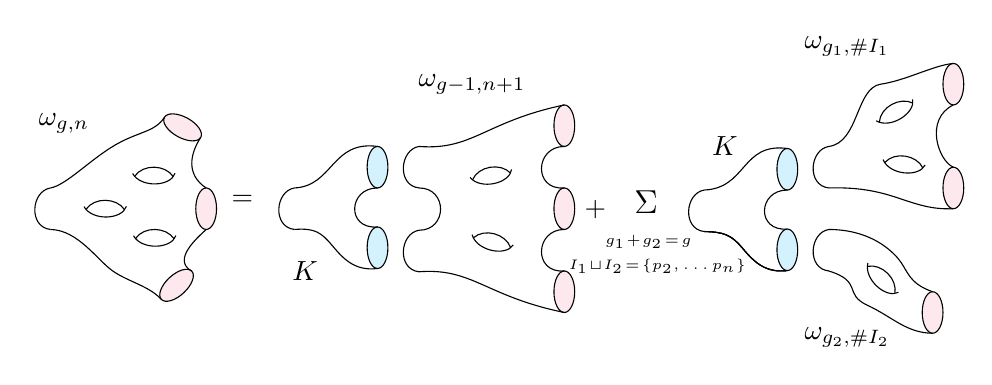
\begin{tikzpicture}[x=0.75pt,y=0.75pt,yscale=-1,xscale=1]
%uncomment if require: \path (0,190); %set diagram left start at 0, and has height of 190

%Shape: Ellipse [id:dp47766951388601575] 
\draw  [fill={rgb, 255:red, 85; green, 205; blue, 252 }  ,fill opacity=0.25 ] (162.56,69.5) .. controls (162.56,63.98) and (164.8,59.5) .. (167.56,59.5) .. controls (170.32,59.5) and (172.56,63.98) .. (172.56,69.5) .. controls (172.56,75.02) and (170.32,79.5) .. (167.56,79.5) .. controls (164.8,79.5) and (162.56,75.02) .. (162.56,69.5) -- cycle ;
%Shape: Ellipse [id:dp2213117305497102] 
\draw  [fill={rgb, 255:red, 85; green, 205; blue, 252 }  ,fill opacity=0.25 ] (162.56,108.3) .. controls (162.56,102.78) and (164.8,98.3) .. (167.56,98.3) .. controls (170.32,98.3) and (172.56,102.78) .. (172.56,108.3) .. controls (172.56,113.83) and (170.32,118.3) .. (167.56,118.3) .. controls (164.8,118.3) and (162.56,113.83) .. (162.56,108.3) -- cycle ;
%Curve Lines [id:da6254818543814082] 
\draw    (127.56,79.5) .. controls (146.2,78.6) and (145.39,56.5) .. (167.56,59.5) ;
%Curve Lines [id:da26678157319223816] 
\draw    (127.56,99.5) .. controls (137.49,98.7) and (140.48,101.08) .. (145.58,107.07) .. controls (150.67,113.06) and (156.21,119.75) .. (167.56,118.3) ;
%Shape: Ellipse [id:dp13037643339418226] 
\draw  [fill={rgb, 255:red, 85; green, 205; blue, 252 }  ,fill opacity=0.25 ] (360,70.5) .. controls (360,64.98) and (362.24,60.5) .. (365,60.5) .. controls (367.76,60.5) and (370,64.98) .. (370,70.5) .. controls (370,76.02) and (367.76,80.5) .. (365,80.5) .. controls (362.24,80.5) and (360,76.02) .. (360,70.5) -- cycle ;
%Shape: Ellipse [id:dp17263407292053756] 
\draw  [fill={rgb, 255:red, 85; green, 205; blue, 252 }  ,fill opacity=0.25 ] (360,109.3) .. controls (360,103.78) and (362.24,99.3) .. (365,99.3) .. controls (367.76,99.3) and (370,103.78) .. (370,109.3) .. controls (370,114.82) and (367.76,119.3) .. (365,119.3) .. controls (362.24,119.3) and (360,114.82) .. (360,109.3) -- cycle ;
%Curve Lines [id:da07654552783686674] 
\draw    (325,80.5) .. controls (345.53,79.6) and (342.83,57.5) .. (365,60.5) ;
%Curve Lines [id:da9658431109856747] 
\draw    (325,100.5) .. controls (334.27,100.7) and (337.92,102.08) .. (343.02,108.07) .. controls (348.11,114.06) and (353.65,120.74) .. (365,119.3) ;
%Curve Lines [id:da5347071930943992] 
\draw    (365,80.5) .. controls (350.83,80.5) and (349.83,100.5) .. (365,99.3) ;
%Shape: Ellipse [id:dp3047856800313534] 
\draw  [fill={rgb, 255:red, 247; green, 168; blue, 184 }  ,fill opacity=0.25 ] (440,29.5) .. controls (440,23.98) and (442.24,19.5) .. (445,19.5) .. controls (447.76,19.5) and (450,23.98) .. (450,29.5) .. controls (450,35.02) and (447.76,39.5) .. (445,39.5) .. controls (442.24,39.5) and (440,35.02) .. (440,29.5) -- cycle ;
%Shape: Ellipse [id:dp604261263939661] 
\draw  [fill={rgb, 255:red, 247; green, 168; blue, 184 }  ,fill opacity=0.25 ] (440,79.5) .. controls (440,73.98) and (442.24,69.5) .. (445,69.5) .. controls (447.76,69.5) and (450,73.98) .. (450,79.5) .. controls (450,85.02) and (447.76,89.5) .. (445,89.5) .. controls (442.24,89.5) and (440,85.02) .. (440,79.5) -- cycle ;
%Shape: Ellipse [id:dp011621115124847092] 
\draw  [fill={rgb, 255:red, 247; green, 168; blue, 184 }  ,fill opacity=0.25 ] (430,139.5) .. controls (430,133.98) and (432.24,129.5) .. (435,129.5) .. controls (437.76,129.5) and (440,133.98) .. (440,139.5) .. controls (440,145.02) and (437.76,149.5) .. (435,149.5) .. controls (432.24,149.5) and (430,145.02) .. (430,139.5) -- cycle ;
%Curve Lines [id:da570536589787372] 
\draw    (385,59.5) .. controls (399.53,57.6) and (397.98,31.23) .. (410,29.5) .. controls (422.02,27.77) and (435.36,20.43) .. (445,19.5) ;
%Curve Lines [id:da47026968306688344] 
\draw    (385,79.5) .. controls (416.83,78.5) and (423.36,90.43) .. (445,89.5) ;
%Curve Lines [id:da10402241670297141] 
\draw    (445,39.5) .. controls (430.83,46.5) and (437.83,66.5) .. (445,69.5) ;
%Curve Lines [id:da7257812222165501] 
\draw    (411.92,67.27) .. controls (416.75,61.8) and (427.35,63.59) .. (430.34,69.91) ;
%Curve Lines [id:da1333862640100011] 
\draw    (411.13,65.82) .. controls (414.17,73.32) and (428.46,74.53) .. (431.39,68.4) ;

%Curve Lines [id:da9669557373363992] 
\draw    (409.32,47.82) .. controls (409.79,40.54) and (419.25,35.45) .. (425.49,38.61) ;
%Curve Lines [id:da3422827424389957] 
\draw    (407.81,47.17) .. controls (414.82,51.22) and (426.83,43.4) .. (425.39,36.77) ;

%Curve Lines [id:da9799334827307091] 
\draw    (385,119.5) .. controls (401.6,124.7) and (391.85,130.63) .. (403.6,136.03) .. controls (415.35,141.43) and (422.35,149.43) .. (435,149.5) ;
%Curve Lines [id:da9139019865430383] 
\draw    (403.59,117.28) .. controls (410.73,115.78) and (418.17,123.53) .. (416.8,130.39) ;
%Curve Lines [id:da4926725298466649] 
\draw    (403.81,115.66) .. controls (401.79,123.49) and (412.53,132.97) .. (418.54,129.8) ;

%Curve Lines [id:da8231578381022252] 
\draw    (385,99.5) .. controls (403.53,99.6) and (413.6,108.03) .. (418.27,113.37) .. controls (422.93,118.7) and (422.93,125.37) .. (435,129.5) ;
%Curve Lines [id:da41952521800040865] 
\draw    (325,80.5) .. controls (315.6,82.03) and (314.27,99.37) .. (325,100.5) ;
%Curve Lines [id:da022423481574913584] 
\draw    (385,59.5) .. controls (375.6,61.03) and (374.27,78.37) .. (385,79.5) ;
%Curve Lines [id:da9251927665164891] 
\draw    (385,99.5) .. controls (375.6,101.03) and (374.27,118.37) .. (385,119.5) ;
%Curve Lines [id:da23000894520127613] 
\draw    (325,100.5) .. controls (334.27,100.7) and (337.92,102.08) .. (343.02,108.07) .. controls (348.11,114.06) and (353.65,120.74) .. (365,119.3) ;
%Curve Lines [id:da10195049737374684] 
\draw    (167.56,79.5) .. controls (153.39,79.5) and (152.39,99.5) .. (167.56,98.3) ;
%Curve Lines [id:da5107062925199526] 
\draw    (187.56,79.5) .. controls (201.39,79.5) and (201.39,99.88) .. (187.56,99.88) ;
%Shape: Ellipse [id:dp3889460224785426] 
\draw  [fill={rgb, 255:red, 247; green, 168; blue, 184 }  ,fill opacity=0.26 ] (252.56,49.5) .. controls (252.56,43.98) and (254.8,39.5) .. (257.56,39.5) .. controls (260.32,39.5) and (262.56,43.98) .. (262.56,49.5) .. controls (262.56,55.02) and (260.32,59.5) .. (257.56,59.5) .. controls (254.8,59.5) and (252.56,55.02) .. (252.56,49.5) -- cycle ;
%Shape: Ellipse [id:dp9770499883484128] 
\draw  [fill={rgb, 255:red, 247; green, 168; blue, 184 }  ,fill opacity=0.25 ] (252.56,89.5) .. controls (252.56,83.98) and (254.8,79.5) .. (257.56,79.5) .. controls (260.32,79.5) and (262.56,83.98) .. (262.56,89.5) .. controls (262.56,95.02) and (260.32,99.5) .. (257.56,99.5) .. controls (254.8,99.5) and (252.56,95.02) .. (252.56,89.5) -- cycle ;
%Shape: Ellipse [id:dp4597094401087267] 
\draw  [fill={rgb, 255:red, 247; green, 168; blue, 184 }  ,fill opacity=0.25 ] (252.56,129.5) .. controls (252.56,123.98) and (254.8,119.5) .. (257.56,119.5) .. controls (260.32,119.5) and (262.56,123.98) .. (262.56,129.5) .. controls (262.56,135.02) and (260.32,139.5) .. (257.56,139.5) .. controls (254.8,139.5) and (252.56,135.02) .. (252.56,129.5) -- cycle ;
%Shape: Boxed Bezier Curve [id:dp4201913915112617] 
\draw    (187.56,59.5) .. controls (213.39,61.5) and (219.39,47.5) .. (257.56,39.5) ;
%Curve Lines [id:da17496795078002492] 
\draw    (257.56,59.5) .. controls (243.39,59.5) and (242.39,80.7) .. (257.56,79.5) ;
%Straight Lines [id:da8933167588243608] 
\draw  [dash pattern={on 4.5pt off 4.5pt}]  (222.56,89.5) ;
%Shape: Boxed Bezier Curve [id:dp20175324397284145] 
\draw    (187.56,119.88) .. controls (213.39,117.92) and (219.39,131.65) .. (257.56,139.5) ;
%Curve Lines [id:da7870873777983136] 
\draw    (257.56,99.5) .. controls (243.39,99.5) and (242.39,120.7) .. (257.56,119.5) ;
%Curve Lines [id:da8945713210334673] 
\draw    (325,100.5) .. controls (334.27,100.7) and (337.92,102.08) .. (343.02,108.07) .. controls (348.11,114.06) and (353.65,120.74) .. (365,119.3) ;
%Curve Lines [id:da6694044469732641] 
\draw    (213.33,75.57) .. controls (216.22,68.88) and (226.84,67.26) .. (231.66,72.34) ;
%Curve Lines [id:da5731533719506826] 
\draw    (212.13,74.45) .. controls (217.37,80.62) and (231.31,77.31) .. (232.18,70.57) ;

%Curve Lines [id:da02679938946556648] 
\draw    (213.73,103.52) .. controls (219.18,98.67) and (229.49,101.69) .. (231.71,108.32) ;
%Curve Lines [id:da8638414158098124] 
\draw    (213.12,102) .. controls (215.26,109.8) and (229.3,112.68) .. (232.93,106.94) ;

%Curve Lines [id:da5955732991885125] 
\draw    (187.56,59.5) .. controls (178.16,61.03) and (176.82,78.37) .. (187.56,79.5) ;
%Curve Lines [id:da21844641699333922] 
\draw    (187.56,99.88) .. controls (178.16,101.42) and (176.82,118.75) .. (187.56,119.88) ;
%Curve Lines [id:da22082602480849645] 
\draw    (127.56,79.5) .. controls (118.16,81.03) and (116.82,98.37) .. (127.56,99.5) ;
%Shape: Ellipse [id:dp047839199679800104] 
\draw  [fill={rgb, 255:red, 247; green, 168; blue, 184 }  ,fill opacity=0.26 ] (76.04,45.92) .. controls (80.88,48.58) and (83.73,52.69) .. (82.4,55.12) .. controls (81.08,57.54) and (76.07,57.35) .. (71.23,54.69) .. controls (66.39,52.04) and (63.54,47.92) .. (64.87,45.5) .. controls (66.19,43.08) and (71.19,43.27) .. (76.04,45.92) -- cycle ;
%Shape: Ellipse [id:dp8497917036559762] 
\draw  [fill={rgb, 255:red, 247; green, 168; blue, 184 }  ,fill opacity=0.26 ] (80,89.5) .. controls (80,83.98) and (82.24,79.5) .. (85,79.5) .. controls (87.76,79.5) and (90,83.98) .. (90,89.5) .. controls (90,95.02) and (87.76,99.5) .. (85,99.5) .. controls (82.24,99.5) and (80,95.02) .. (80,89.5) -- cycle ;
%Curve Lines [id:da21030774171420585] 
\draw    (27.11,89.81) .. controls (31.19,83.76) and (41.93,84.15) .. (45.72,90.03) ;
%Curve Lines [id:da2054533399102827] 
\draw    (26.14,88.48) .. controls (30.14,95.52) and (44.45,94.85) .. (46.56,88.39) ;

%Curve Lines [id:da2922985882802336] 
\draw    (50.55,73.87) .. controls (54.63,67.82) and (65.37,68.2) .. (69.16,74.08) ;
%Curve Lines [id:da7481414220068059] 
\draw    (49.58,72.54) .. controls (53.58,79.58) and (67.89,78.9) .. (70,72.45) ;

%Curve Lines [id:da19338719689530326] 
\draw    (50.97,103.87) .. controls (55.05,97.82) and (65.79,98.2) .. (69.58,104.08) ;
%Curve Lines [id:da4856907558404082] 
\draw    (50,102.54) .. controls (54,109.58) and (68.32,108.9) .. (70.42,102.45) ;

%Shape: Ellipse [id:dp5786014847995782] 
\draw  [fill={rgb, 255:red, 247; green, 168; blue, 184 }  ,fill opacity=0.26 ] (74.13,130.06) .. controls (70.07,133.81) and (65.27,135.2) .. (63.39,133.17) .. controls (61.52,131.14) and (63.29,126.46) .. (67.35,122.71) .. controls (71.4,118.97) and (76.21,117.57) .. (78.08,119.6) .. controls (79.96,121.63) and (78.19,126.31) .. (74.13,130.06) -- cycle ;
%Curve Lines [id:da5518785962687732] 
\draw    (10,79.5) .. controls (0.6,81.03) and (-0.73,98.37) .. (10,99.5) ;
%Curve Lines [id:da9074172955656375] 
\draw    (10,99.5) .. controls (23.24,99.75) and (32.51,114.27) .. (40,119.5) .. controls (47.49,124.73) and (57.39,126.65) .. (63.39,133.17) ;
%Curve Lines [id:da4486713212196154] 
\draw    (10,79.5) .. controls (17.34,78.17) and (28.21,66.73) .. (40,59.5) .. controls (51.79,52.27) and (60.13,52.87) .. (64.87,45.5) ;
%Curve Lines [id:da29408206197280085] 
\draw    (82.4,55.12) .. controls (77.2,63.1) and (75.2,73.1) .. (85,79.5) ;
%Curve Lines [id:da06937876092619744] 
\draw    (85,99.5) .. controls (81.2,103.1) and (68.2,114.1) .. (78.08,119.6) ;

% Text Node
\draw (272.5,90) node    {$+$};
% Text Node
\draw (298,105.5) node  [font=\tiny]  {$g_{1}\! + \! g_{2} \! = \! g$};
% Text Node
\draw (213.12,29.5) node    {$\omega _{g-1,n+1}$};
% Text Node
\draw (393.94,11.5) node    {$\omega _{g_{1} ,\#I_{1}}$};
% Text Node
\draw (132.62,119.5) node    {$K$};
% Text Node
\draw (393.94,151.5) node    {$\omega _{g_{2} ,\#I_{2}}$};
% Text Node
\draw (334.94,59.5) node    {$K$};
% Text Node
\draw (96,81.9) node [anchor=north west][inner sep=0.75pt]    {$=$};
% Text Node
\draw (16.5,48.5) node    {$\omega _{g,n}$};
% Text Node
\draw (258.44,112.4) node [anchor=north west][inner sep=0.75pt]  [font=\tiny]  {$I_{1} \! \sqcup \! I_{2}\! = \!\{p_{2}, \dots p_{n} \}$};
% Text Node
\draw (290,79.4) node [anchor=north west][inner sep=0.75pt]  [font=\large]  {$\Sigma $};
\end{tikzpicture}

        \caption{A diagrammatic overview of topological recursion. In this picture \(g=n=3\), and only one combination for \(g_1\) and \(g_2\) is displayed. Boundaries, drawn as a shaded ellipses represents the number \(n\). Internal holes represent the genus \(g\). }
        \label{fig:tr}
    \end{figure}
    As seen in figure (\ref{fig:tr}), each \( \omega_{g,n}\) can be thought of as having an extra boundary that is capped off. \( K\) is visualised as an object with two free boundaries, no holes (the genus), and a capped boundary, like a pair of pants. \( \omega_{g,n}\) has \(n\) free boundaries, and \(1\) capped boundary. When \( \omega_{\sbt,\sbt}\) is joined with a \(K\) term, that cap is removed exposing a boundary which is glued with a leg of the \(K\) term. For the \( \omega_{g-1,n+1}\) term the uncapped boundary, or a fixed boundary, and a free external boundary join with the free boundaries of \(K\) to increase the genus, for example figure (\ref{fig:trcut}). The \( \omega_{g_1, \sbt}\) and \( \omega_{g_2,\sbt}\) are joined at the uncapped boundary with a \(K\) increasing the free boundaries.
    \begin{figure}[!htb]
        \centering 
        

\tikzset{every picture/.style={line width=0.75pt}} %set default line width to 0.75pt        

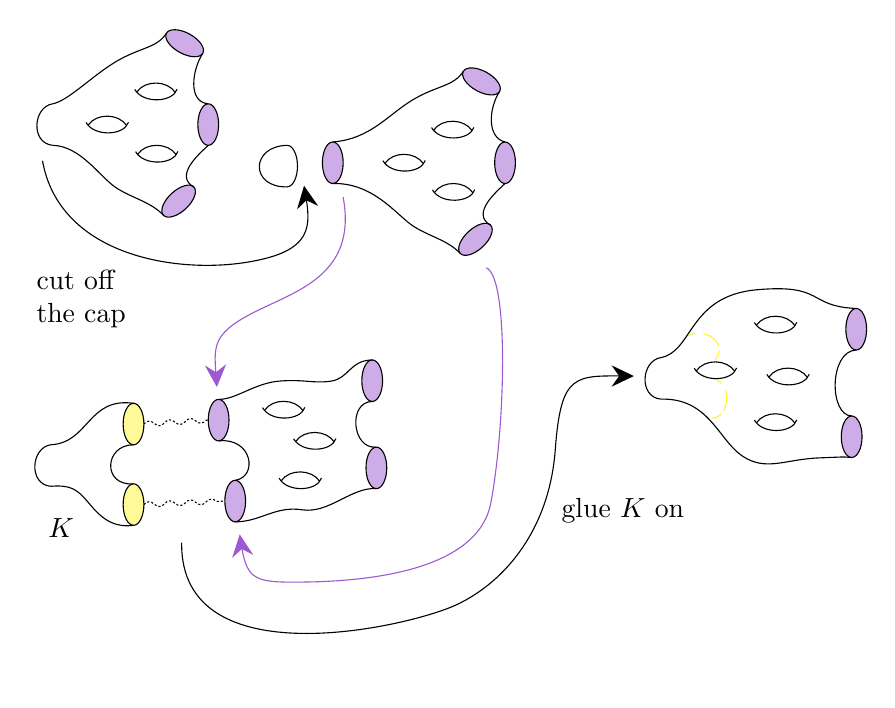
\begin{tikzpicture}[x=0.75pt,y=0.75pt,yscale=-1,xscale=1]
%uncomment if require: \path (0,366); %set diagram left start at 0, and has height of 366

%Curve Lines [id:da7456363211127895] 
\draw [color={rgb, 255:red, 255; green, 244; blue, 48 }  ,draw opacity=1 ] [dash pattern={on 3.75pt off 3pt on 7.5pt off 1.5pt}]  (325,164.55) .. controls (332.1,158.61) and (347.35,166.61) .. (338.45,176.18) ;
%Curve Lines [id:da21755327461639118] 
\draw [color={rgb, 255:red, 255; green, 244; blue, 48 }  ,draw opacity=1 ] [dash pattern={on 3.75pt off 3pt on 7.5pt off 1.5pt}]  (338,184.3) .. controls (349.35,186.86) and (345.2,206.93) .. (335.2,202.9) ;
%Shape: Ellipse [id:dp47766951388601575] 
\draw  [fill={rgb, 255:red, 255; green, 244; blue, 48 }  ,fill opacity=0.5 ] (54,206.28) .. controls (54,200.76) and (56.24,196.28) .. (59,196.28) .. controls (61.76,196.28) and (64,200.76) .. (64,206.28) .. controls (64,211.8) and (61.76,216.28) .. (59,216.28) .. controls (56.24,216.28) and (54,211.8) .. (54,206.28) -- cycle ;
%Shape: Ellipse [id:dp2213117305497102] 
\draw  [fill={rgb, 255:red, 255; green, 244; blue, 48 }  ,fill opacity=0.5 ] (54,245.08) .. controls (54,239.56) and (56.24,235.08) .. (59,235.08) .. controls (61.76,235.08) and (64,239.56) .. (64,245.08) .. controls (64,250.6) and (61.76,255.08) .. (59,255.08) .. controls (56.24,255.08) and (54,250.6) .. (54,245.08) -- cycle ;
%Curve Lines [id:da6254818543814082] 
\draw    (19,216.28) .. controls (37.64,215.38) and (36.83,193.28) .. (59,196.28) ;
%Curve Lines [id:da26678157319223816] 
\draw    (19,236.28) .. controls (28.93,235.48) and (31.92,237.86) .. (37.02,243.85) .. controls (42.11,249.84) and (47.65,256.53) .. (59,255.08) ;
%Curve Lines [id:da10195049737374684] 
\draw    (59,216.28) .. controls (44.83,216.28) and (43.83,236.28) .. (59,235.08) ;
%Curve Lines [id:da22082602480849645] 
\draw    (19,216.28) .. controls (9.6,217.81) and (8.27,235.15) .. (19,236.28) ;
%Shape: Ellipse [id:dp047839199679800104] 
\draw  [fill={rgb, 255:red, 156; green, 89; blue, 209 }  ,fill opacity=0.5 ] (229.04,36.82) .. controls (233.88,39.47) and (236.73,43.59) .. (235.4,46.01) .. controls (234.08,48.43) and (229.07,48.24) .. (224.23,45.59) .. controls (219.39,42.93) and (216.54,38.82) .. (217.87,36.4) .. controls (219.19,33.98) and (224.19,34.16) .. (229.04,36.82) -- cycle ;
%Shape: Ellipse [id:dp8497917036559762] 
\draw  [fill={rgb, 255:red, 156; green, 89; blue, 209 }  ,fill opacity=0.5 ] (233,80.4) .. controls (233,74.87) and (235.24,70.4) .. (238,70.4) .. controls (240.76,70.4) and (243,74.87) .. (243,80.4) .. controls (243,85.92) and (240.76,90.4) .. (238,90.4) .. controls (235.24,90.4) and (233,85.92) .. (233,80.4) -- cycle ;
%Curve Lines [id:da21030774171420585] 
\draw    (180.11,80.7) .. controls (184.19,74.66) and (194.93,75.04) .. (198.72,80.92) ;
%Curve Lines [id:da2054533399102827] 
\draw    (179.14,79.38) .. controls (183.14,86.42) and (197.45,85.74) .. (199.56,79.28) ;

%Curve Lines [id:da2922985882802336] 
\draw    (203.55,64.76) .. controls (207.63,58.71) and (218.37,59.1) .. (222.16,64.98) ;
%Curve Lines [id:da7481414220068059] 
\draw    (202.58,63.44) .. controls (206.58,70.47) and (220.89,69.8) .. (223,63.34) ;

%Curve Lines [id:da19338719689530326] 
\draw    (203.97,94.76) .. controls (208.05,88.71) and (218.79,89.1) .. (222.58,94.98) ;
%Curve Lines [id:da4856907558404082] 
\draw    (203,93.44) .. controls (207,100.47) and (221.32,99.8) .. (223.42,93.34) ;

%Shape: Ellipse [id:dp5786014847995782] 
\draw  [fill={rgb, 255:red, 156; green, 89; blue, 209 }  ,fill opacity=0.5 ] (227.13,120.96) .. controls (223.07,124.7) and (218.27,126.1) .. (216.39,124.07) .. controls (214.52,122.04) and (216.29,117.36) .. (220.35,113.61) .. controls (224.4,109.86) and (229.21,108.47) .. (231.08,110.5) .. controls (232.96,112.53) and (231.19,117.21) .. (227.13,120.96) -- cycle ;
%Curve Lines [id:da9074172955656375] 
\draw    (155,90.4) .. controls (174.15,89.85) and (185.51,105.16) .. (193,110.4) .. controls (200.49,115.63) and (210.39,117.55) .. (216.39,124.07) ;
%Curve Lines [id:da4486713212196154] 
\draw    (155,70.4) .. controls (173.15,68.85) and (181.21,57.63) .. (193,50.4) .. controls (204.79,43.17) and (213.13,43.77) .. (217.87,36.4) ;
%Curve Lines [id:da29408206197280085] 
\draw    (235.4,46.01) .. controls (230.2,54) and (229.05,68.15) .. (238,70.4) ;
%Curve Lines [id:da06937876092619744] 
\draw    (238,90.4) .. controls (234.2,94) and (221.2,105) .. (231.08,110.5) ;
%Shape: Ellipse [id:dp5834692450385205] 
\draw  [fill={rgb, 255:red, 156; green, 89; blue, 209 }  ,fill opacity=0.5 ] (86.04,18.42) .. controls (90.88,21.08) and (93.73,25.19) .. (92.4,27.62) .. controls (91.08,30.04) and (86.07,29.85) .. (81.23,27.19) .. controls (76.39,24.54) and (73.54,20.42) .. (74.87,18) .. controls (76.19,15.58) and (81.19,15.77) .. (86.04,18.42) -- cycle ;
%Shape: Ellipse [id:dp9981691356596056] 
\draw  [fill={rgb, 255:red, 156; green, 89; blue, 209 }  ,fill opacity=0.5 ] (90,62) .. controls (90,56.48) and (92.24,52) .. (95,52) .. controls (97.76,52) and (100,56.48) .. (100,62) .. controls (100,67.52) and (97.76,72) .. (95,72) .. controls (92.24,72) and (90,67.52) .. (90,62) -- cycle ;
%Curve Lines [id:da7930767734111239] 
\draw    (37.11,62.31) .. controls (41.19,56.26) and (51.93,56.65) .. (55.72,62.53) ;
%Curve Lines [id:da23296535928943463] 
\draw    (36.14,60.98) .. controls (40.14,68.02) and (54.45,67.35) .. (56.56,60.89) ;

%Curve Lines [id:da5658450019102096] 
\draw    (60.55,46.37) .. controls (64.63,40.32) and (75.37,40.7) .. (79.16,46.58) ;
%Curve Lines [id:da37655485995425364] 
\draw    (59.58,45.04) .. controls (63.58,52.08) and (77.89,51.4) .. (80,44.95) ;

%Curve Lines [id:da38704533910669703] 
\draw    (60.97,76.37) .. controls (65.05,70.32) and (75.79,70.7) .. (79.58,76.58) ;
%Curve Lines [id:da8417748691785382] 
\draw    (60,75.04) .. controls (64,82.08) and (78.32,81.4) .. (80.42,74.95) ;

%Shape: Ellipse [id:dp5782111136495405] 
\draw  [fill={rgb, 255:red, 156; green, 89; blue, 209 }  ,fill opacity=0.5 ] (84.13,102.56) .. controls (80.07,106.31) and (75.27,107.7) .. (73.39,105.67) .. controls (71.52,103.64) and (73.29,98.96) .. (77.35,95.21) .. controls (81.4,91.47) and (86.21,90.07) .. (88.08,92.1) .. controls (89.96,94.13) and (88.19,98.81) .. (84.13,102.56) -- cycle ;
%Curve Lines [id:da05841297602590634] 
\draw    (20,52) .. controls (10.6,53.53) and (9.27,70.87) .. (20,72) ;
%Curve Lines [id:da8590000152828204] 
\draw    (20,72) .. controls (33.24,72.25) and (42.51,86.77) .. (50,92) .. controls (57.49,97.23) and (67.39,99.15) .. (73.39,105.67) ;
%Curve Lines [id:da24903761379144307] 
\draw    (20,52) .. controls (27.34,50.67) and (38.21,39.23) .. (50,32) .. controls (61.79,24.77) and (70.13,25.37) .. (74.87,18) ;
%Curve Lines [id:da4778043785246958] 
\draw    (92.4,27.62) .. controls (87.2,35.6) and (85.05,51.15) .. (95,52) ;
%Curve Lines [id:da37177679505336103] 
\draw    (95,72) .. controls (91.2,75.6) and (78.2,86.6) .. (88.08,92.1) ;
%Curve Lines [id:da06243127894946254] 
\draw    (15.15,79.45) .. controls (23.15,124.45) and (78.05,133.95) .. (113.2,128.4) .. controls (146.42,123.16) and (144.4,110.63) .. (141.63,94.33) ;
\draw [shift={(141.15,91.45)}, rotate = 80.7] [fill={rgb, 255:red, 0; green, 0; blue, 0 }  ][line width=0.08]  [draw opacity=0] (10.72,-5.15) -- (0,0) -- (10.72,5.15) -- (7.12,0) -- cycle    ;
%Shape: Ellipse [id:dp8212226002047514] 
\draw  [fill={rgb, 255:red, 156; green, 89; blue, 209 }  ,fill opacity=0.5 ] (150,80.4) .. controls (150,74.87) and (152.24,70.4) .. (155,70.4) .. controls (157.76,70.4) and (160,74.87) .. (160,80.4) .. controls (160,85.92) and (157.76,90.4) .. (155,90.4) .. controls (152.24,90.4) and (150,85.92) .. (150,80.4) -- cycle ;
%Shape: Arc [id:dp4052834836534003] 
\draw  [draw opacity=0] (133,72) .. controls (133,72) and (133,72) .. (133,72) .. controls (133,72) and (133,72) .. (133,72) .. controls (135.76,72) and (138,76.48) .. (138,82) .. controls (138,87.52) and (135.76,92) .. (133,92) -- (133,82) -- cycle ; \draw   (133,72) .. controls (133,72) and (133,72) .. (133,72) .. controls (133,72) and (133,72) .. (133,72) .. controls (135.76,72) and (138,76.48) .. (138,82) .. controls (138,87.52) and (135.76,92) .. (133,92) ;  
%Curve Lines [id:da08409869661196623] 
\draw    (133,72) .. controls (115.15,72.45) and (115.15,92.45) .. (133,92) ;
%Curve Lines [id:da9204492733817433] 
\draw [color={rgb, 255:red, 156; green, 89; blue, 209 }  ,draw opacity=1 ]   (160,97) .. controls (167.17,135.65) and (135.35,142.65) .. (115.2,153.4) .. controls (96.16,163.56) and (97.79,169.48) .. (98.96,185.54) ;
\draw [shift={(99.15,188.45)}, rotate = 266.56] [fill={rgb, 255:red, 156; green, 89; blue, 209 }  ,fill opacity=1 ][line width=0.08]  [draw opacity=0] (10.72,-5.15) -- (0,0) -- (10.72,5.15) -- (7.12,0) -- cycle    ;
%Shape: Ellipse [id:dp776754946890608] 
\draw  [fill={rgb, 255:red, 156; green, 89; blue, 209 }  ,fill opacity=0.5 ] (95,204.4) .. controls (95,198.87) and (97.24,194.4) .. (100,194.4) .. controls (102.76,194.4) and (105,198.87) .. (105,204.4) .. controls (105,209.92) and (102.76,214.4) .. (100,214.4) .. controls (97.24,214.4) and (95,209.92) .. (95,204.4) -- cycle ;
%Shape: Ellipse [id:dp199266464828314] 
\draw  [fill={rgb, 255:red, 156; green, 89; blue, 209 }  ,fill opacity=0.5 ] (103,243.4) .. controls (103,237.87) and (105.24,233.4) .. (108,233.4) .. controls (110.76,233.4) and (113,237.87) .. (113,243.4) .. controls (113,248.92) and (110.76,253.4) .. (108,253.4) .. controls (105.24,253.4) and (103,248.92) .. (103,243.4) -- cycle ;
%Shape: Ellipse [id:dp645631326139301] 
\draw  [fill={rgb, 255:red, 156; green, 89; blue, 209 }  ,fill opacity=0.5 ] (169,185.4) .. controls (169,179.87) and (171.24,175.4) .. (174,175.4) .. controls (176.76,175.4) and (179,179.87) .. (179,185.4) .. controls (179,190.92) and (176.76,195.4) .. (174,195.4) .. controls (171.24,195.4) and (169,190.92) .. (169,185.4) -- cycle ;
%Shape: Ellipse [id:dp6611377988217855] 
\draw  [fill={rgb, 255:red, 156; green, 89; blue, 209 }  ,fill opacity=0.5 ] (171,227.4) .. controls (171,221.87) and (173.24,217.4) .. (176,217.4) .. controls (178.76,217.4) and (181,221.87) .. (181,227.4) .. controls (181,232.92) and (178.76,237.4) .. (176,237.4) .. controls (173.24,237.4) and (171,232.92) .. (171,227.4) -- cycle ;
%Curve Lines [id:da27596733021021924] 
\draw    (122.11,199.7) .. controls (126.19,193.66) and (136.93,194.04) .. (140.72,199.92) ;
%Curve Lines [id:da749269569119316] 
\draw    (121.14,198.38) .. controls (125.14,205.42) and (139.45,204.74) .. (141.56,198.28) ;

%Curve Lines [id:da4284732853055516] 
\draw    (137.11,214.7) .. controls (141.19,208.66) and (151.93,209.04) .. (155.72,214.92) ;
%Curve Lines [id:da23097840362923172] 
\draw    (136.14,213.38) .. controls (140.14,220.42) and (154.45,219.74) .. (156.56,213.28) ;

%Curve Lines [id:da208706920085994] 
\draw    (130.11,233.7) .. controls (134.19,227.66) and (144.93,228.04) .. (148.72,233.92) ;
%Curve Lines [id:da8277159491807085] 
\draw    (129.14,232.38) .. controls (133.14,239.42) and (147.45,238.74) .. (149.56,232.28) ;

%Curve Lines [id:da3865559692174718] 
\draw [color={rgb, 255:red, 156; green, 89; blue, 209 }  ,draw opacity=1 ]   (229,131) .. controls (239.93,135.66) and (238.15,207.25) .. (231.15,244.25) .. controls (224.15,281.25) and (157.2,282.4) .. (136.15,282.45) .. controls (116.05,282.5) and (113.27,280.36) .. (110.54,262.13) ;
\draw [shift={(110.15,259.45)}, rotate = 82.02] [fill={rgb, 255:red, 156; green, 89; blue, 209 }  ,fill opacity=1 ][line width=0.08]  [draw opacity=0] (10.72,-5.15) -- (0,0) -- (10.72,5.15) -- (7.12,0) -- cycle    ;
%Straight Lines [id:da364586372920236] 
\draw  [dash pattern={on 0.75pt off 0.75pt}]  (64,206.28) .. controls (65.57,204.51) and (67.23,204.41) .. (68.99,205.98) .. controls (70.76,207.54) and (72.42,207.44) .. (73.98,205.67) .. controls (75.54,203.9) and (77.2,203.8) .. (78.97,205.37) .. controls (80.74,206.94) and (82.4,206.84) .. (83.96,205.07) .. controls (85.52,203.3) and (87.18,203.2) .. (88.95,204.76) .. controls (90.72,206.33) and (92.38,206.23) .. (93.94,204.46) -- (95,204.4) -- (95,204.4) ;
%Straight Lines [id:da9532142435486358] 
\draw  [dash pattern={on 0.75pt off 0.75pt}]  (64,245.08) .. controls (65.59,243.35) and (67.26,243.28) .. (69,244.87) .. controls (70.74,246.46) and (72.4,246.39) .. (73.99,244.65) .. controls (75.58,242.91) and (77.25,242.84) .. (78.99,244.43) .. controls (80.72,246.02) and (82.39,245.95) .. (83.98,244.22) .. controls (85.57,242.48) and (87.24,242.41) .. (88.98,244) .. controls (90.71,245.59) and (92.38,245.52) .. (93.97,243.79) .. controls (95.56,242.05) and (97.23,241.98) .. (98.97,243.57) -- (103,243.4) -- (103,243.4) ;
%Curve Lines [id:da521532194512972] 
\draw    (100,194.4) .. controls (108.37,194.49) and (117.2,186.6) .. (129.2,185.6) .. controls (141.2,184.6) and (145.61,186.88) .. (154.2,185.6) .. controls (162.79,184.32) and (163.2,175.6) .. (174,175.4) ;
%Curve Lines [id:da6609977290169392] 
\draw    (100,214.4) .. controls (116.2,212.6) and (119.2,231.6) .. (108,233.4) ;
%Curve Lines [id:da995936588792983] 
\draw    (108,253.4) .. controls (120.2,253.4) and (127.2,245.6) .. (140.2,247.6) .. controls (153.2,249.6) and (164.14,236.46) .. (176,237.4) ;
%Curve Lines [id:da8490538991920554] 
\draw    (174,195.4) .. controls (162.2,195.6) and (164.2,218.6) .. (176,217.4) ;
%Curve Lines [id:da5179124360374171] 
\draw [color={rgb, 255:red, 0; green, 0; blue, 0 }  ,draw opacity=1 ]   (82.2,263.4) .. controls (81.2,329.4) and (192.05,304.15) .. (215.05,293.15) .. controls (238.05,282.15) and (259.35,257.05) .. (262.2,218.6) .. controls (264.95,181.5) and (271.57,182.99) .. (297.19,183.14) ;
\draw [shift={(300.05,183.15)}, rotate = 180] [fill={rgb, 255:red, 0; green, 0; blue, 0 }  ,fill opacity=1 ][line width=0.08]  [draw opacity=0] (10.72,-5.15) -- (0,0) -- (10.72,5.15) -- (7.12,0) -- cycle    ;
%Curve Lines [id:da9066189595509849] 
\draw    (313,174.28) .. controls (303.6,175.81) and (302.27,193.15) .. (313,194.28) ;
%Shape: Ellipse [id:dp1720032696838898] 
\draw  [fill={rgb, 255:red, 156; green, 89; blue, 209 }  ,fill opacity=0.5 ] (402.2,160.6) .. controls (402.2,155.08) and (404.44,150.6) .. (407.2,150.6) .. controls (409.96,150.6) and (412.2,155.08) .. (412.2,160.6) .. controls (412.2,166.12) and (409.96,170.6) .. (407.2,170.6) .. controls (404.44,170.6) and (402.2,166.12) .. (402.2,160.6) -- cycle ;
%Shape: Ellipse [id:dp5828118842225084] 
\draw  [fill={rgb, 255:red, 156; green, 89; blue, 209 }  ,fill opacity=0.5 ] (400,212.4) .. controls (400,206.87) and (402.24,202.4) .. (405,202.4) .. controls (407.76,202.4) and (410,206.87) .. (410,212.4) .. controls (410,217.92) and (407.76,222.4) .. (405,222.4) .. controls (402.24,222.4) and (400,217.92) .. (400,212.4) -- cycle ;
%Curve Lines [id:da12748011779331514] 
\draw    (359.11,158.7) .. controls (363.19,152.66) and (373.93,153.04) .. (377.72,158.92) ;
%Curve Lines [id:da6587047534533921] 
\draw    (358.14,157.38) .. controls (362.14,164.42) and (376.45,163.74) .. (378.56,157.28) ;

%Curve Lines [id:da37914622908130136] 
\draw    (365.11,183.7) .. controls (369.19,177.66) and (379.93,178.04) .. (383.72,183.92) ;
%Curve Lines [id:da09849809070853266] 
\draw    (364.14,182.38) .. controls (368.14,189.42) and (382.45,188.74) .. (384.56,182.28) ;

%Curve Lines [id:da7128015832866221] 
\draw    (359.11,205.7) .. controls (363.19,199.66) and (373.93,200.04) .. (377.72,205.92) ;
%Curve Lines [id:da443803466114602] 
\draw    (358.14,204.38) .. controls (362.14,211.42) and (376.45,210.74) .. (378.56,204.28) ;

%Curve Lines [id:da9774803119180495] 
\draw    (330.11,180.7) .. controls (334.19,174.66) and (344.93,175.04) .. (348.72,180.92) ;
%Curve Lines [id:da010681509366633035] 
\draw    (329.14,179.38) .. controls (333.14,186.42) and (347.45,185.74) .. (349.56,179.28) ;

%Curve Lines [id:da8204011461116862] 
\draw    (313,194.28) .. controls (336.2,193.6) and (340.77,213.84) .. (352.2,221.6) .. controls (363.63,229.36) and (372.89,223.22) .. (389.2,222.6) .. controls (405.51,221.98) and (398.97,222.05) .. (405,222.4) ;
%Curve Lines [id:da13590361013687124] 
\draw    (313,174.28) .. controls (328.63,171.43) and (326.2,144.6) .. (359.2,141.6) .. controls (392.2,138.6) and (383.4,149.6) .. (407.2,150.6) ;
%Curve Lines [id:da4501000826918429] 
\draw    (407.2,170.6) .. controls (394.05,171.15) and (394.05,202.15) .. (405,202.4) ;

% Text Node
\draw (24.06,256.28) node    {$K$};
% Text Node
\draw (264,240.8) node [anchor=north west][inner sep=0.75pt]   [align=left] {glue $\displaystyle K$ on};
% Text Node
\draw (11,131) node [anchor=north west][inner sep=0.75pt]   [align=left] {cut off \\the cap };


\end{tikzpicture}

        \caption{An \( \omega_{g,n}\) having a cap removed before being glued to \(K\) to increase the genus.}
        \label{fig:trcut}
    \end{figure}
    
    Visually, imagine setting the width of the tubes in the picture to zero, to produce graphs of various genus, where a boundary becomes an external vertex in the graph, and the genus of the blob matches the genus of the graph. Also consider the cap as a specially labelled external vertex or a root. Of course, there is a potential ambiguity, there are multiple graphs of genus \(g\). One constraint that will need to be imposed is that all internal vertices will be degree \(3\). Then instead of a single graph, it will then be the case that \(\omega_{g,n}\) is decomposed into a weighted sum of these possible options. For example figure (\ref{fig:trprim}), \( \omega_{2,3}\) will correspond to a sum of these graphs plus permutations. These graphs are distinct from the graphical sums considered usually for topological recursion \cite{eynard_orantin}. Airy structures will describe this procedure. 
    \begin{figure}[!htb]
        \centering 
        

\tikzset{every picture/.style={line width=0.75pt}} %set default line width to 0.75pt        

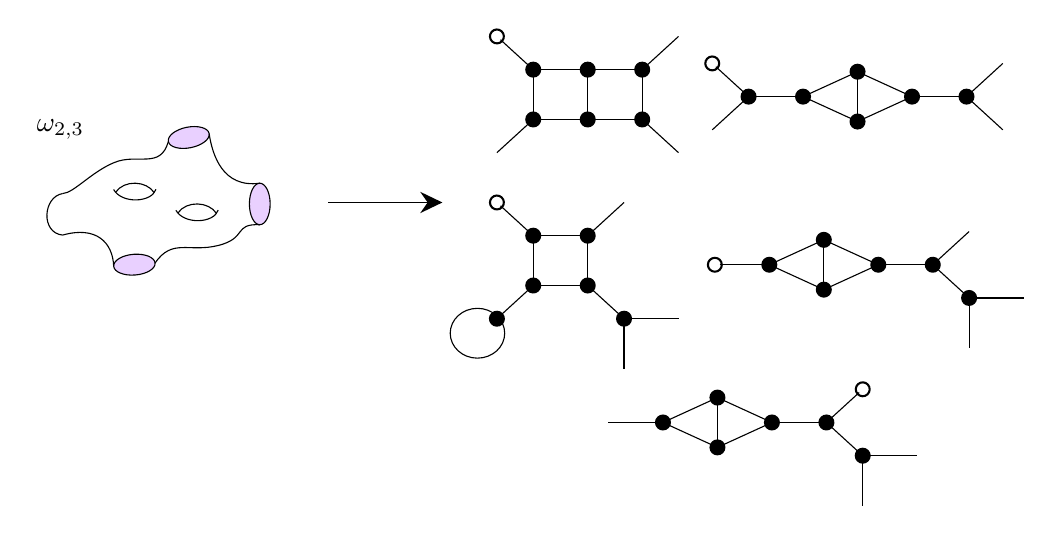
\begin{tikzpicture}[x=0.75pt,y=0.75pt,yscale=-1,xscale=1]
%uncomment if require: \path (0,261); %set diagram left start at 0, and has height of 261

%Straight Lines [id:da5122725041953835] 
\draw    (273.75,55) -- (300,55) ;
\draw [shift={(300,55)}, rotate = 0] [color={rgb, 255:red, 0; green, 0; blue, 0 }  ][fill={rgb, 255:red, 0; green, 0; blue, 0 }  ][line width=0.75]      (0, 0) circle [x radius= 3.35, y radius= 3.35]   ;
\draw [shift={(273.75,55)}, rotate = 0] [color={rgb, 255:red, 0; green, 0; blue, 0 }  ][fill={rgb, 255:red, 0; green, 0; blue, 0 }  ][line width=0.75]      (0, 0) circle [x radius= 3.35, y radius= 3.35]   ;
%Straight Lines [id:da28474322327009105] 
\draw    (273.75,31) -- (300,31) ;
\draw [shift={(300,31)}, rotate = 0] [color={rgb, 255:red, 0; green, 0; blue, 0 }  ][fill={rgb, 255:red, 0; green, 0; blue, 0 }  ][line width=0.75]      (0, 0) circle [x radius= 3.35, y radius= 3.35]   ;
\draw [shift={(273.75,31)}, rotate = 0] [color={rgb, 255:red, 0; green, 0; blue, 0 }  ][fill={rgb, 255:red, 0; green, 0; blue, 0 }  ][line width=0.75]      (0, 0) circle [x radius= 3.35, y radius= 3.35]   ;
%Straight Lines [id:da10829389002897793] 
\draw    (300,31) -- (326.25,31) ;
%Straight Lines [id:da2680222353656253] 
\draw    (300,31) -- (300,55) ;
%Straight Lines [id:da3878078948480259] 
\draw    (273.75,31) -- (273.75,55) ;
%Straight Lines [id:da8964050542040451] 
\draw    (343.75,15) -- (326.25,31) ;
%Straight Lines [id:da2090118876269007] 
\draw    (326.25,55) -- (300,55) ;
%Straight Lines [id:da7172980906443349] 
\draw    (326.25,31) -- (326.25,55) ;
\draw [shift={(326.25,55)}, rotate = 90] [color={rgb, 255:red, 0; green, 0; blue, 0 }  ][fill={rgb, 255:red, 0; green, 0; blue, 0 }  ][line width=0.75]      (0, 0) circle [x radius= 3.35, y radius= 3.35]   ;
\draw [shift={(326.25,31)}, rotate = 90] [color={rgb, 255:red, 0; green, 0; blue, 0 }  ][fill={rgb, 255:red, 0; green, 0; blue, 0 }  ][line width=0.75]      (0, 0) circle [x radius= 3.35, y radius= 3.35]   ;
%Straight Lines [id:da8298682809994327] 
\draw    (343.75,71) -- (326.25,55) ;
%Straight Lines [id:da7340542571833397] 
\draw    (273.75,135) -- (256.25,151) ;
\draw [shift={(256.25,151)}, rotate = 137.56] [color={rgb, 255:red, 0; green, 0; blue, 0 }  ][fill={rgb, 255:red, 0; green, 0; blue, 0 }  ][line width=0.75]      (0, 0) circle [x radius= 3.35, y radius= 3.35]   ;
\draw [shift={(273.75,135)}, rotate = 137.56] [color={rgb, 255:red, 0; green, 0; blue, 0 }  ][fill={rgb, 255:red, 0; green, 0; blue, 0 }  ][line width=0.75]      (0, 0) circle [x radius= 3.35, y radius= 3.35]   ;
%Shape: Ellipse [id:dp8951997570910564] 
\draw   (233.75,158) .. controls (233.75,151.37) and (239.63,146) .. (246.88,146) .. controls (254.12,146) and (260,151.37) .. (260,158) .. controls (260,164.63) and (254.12,170) .. (246.88,170) .. controls (239.63,170) and (233.75,164.63) .. (233.75,158) -- cycle ;
%Straight Lines [id:da30041493250608486] 
\draw    (273.75,135) -- (273.75,111) ;
\draw [shift={(273.75,111)}, rotate = 270] [color={rgb, 255:red, 0; green, 0; blue, 0 }  ][fill={rgb, 255:red, 0; green, 0; blue, 0 }  ][line width=0.75]      (0, 0) circle [x radius= 3.35, y radius= 3.35]   ;
%Straight Lines [id:da06815777790639788] 
\draw    (273.75,135) -- (300,135) ;
\draw [shift={(300,135)}, rotate = 0] [color={rgb, 255:red, 0; green, 0; blue, 0 }  ][fill={rgb, 255:red, 0; green, 0; blue, 0 }  ][line width=0.75]      (0, 0) circle [x radius= 3.35, y radius= 3.35]   ;
%Straight Lines [id:da39270668609938153] 
\draw    (273.75,111) -- (300,111) ;
%Straight Lines [id:da7632138968433353] 
\draw    (300,111) -- (300,135) ;
\draw [shift={(300,111)}, rotate = 90] [color={rgb, 255:red, 0; green, 0; blue, 0 }  ][fill={rgb, 255:red, 0; green, 0; blue, 0 }  ][line width=0.75]      (0, 0) circle [x radius= 3.35, y radius= 3.35]   ;
%Straight Lines [id:da5129578501641567] 
\draw    (300,135) -- (317.5,151) ;
%Straight Lines [id:da3795104652375495] 
\draw    (317.5,151) -- (317.5,175) ;
%Straight Lines [id:da36668627460221803] 
\draw    (317.5,151) -- (343.75,151) ;
\draw [shift={(317.5,151)}, rotate = 0] [color={rgb, 255:red, 0; green, 0; blue, 0 }  ][fill={rgb, 255:red, 0; green, 0; blue, 0 }  ][line width=0.75]      (0, 0) circle [x radius= 3.35, y radius= 3.35]   ;
%Straight Lines [id:da04810774235669735] 
\draw    (257.98,96.59) -- (273.75,111) ;
\draw [shift={(256.25,95)}, rotate = 42.44] [color={rgb, 255:red, 0; green, 0; blue, 0 }  ][line width=0.75]      (0, 0) circle [x radius= 3.35, y radius= 3.35]   ;
%Straight Lines [id:da3040121567882321] 
\draw    (273.75,55) -- (256.25,71) ;
%Straight Lines [id:da8929796050220722] 
\draw    (257.98,16.59) -- (273.75,31) ;
\draw [shift={(256.25,15)}, rotate = 42.44] [color={rgb, 255:red, 0; green, 0; blue, 0 }  ][line width=0.75]      (0, 0) circle [x radius= 3.35, y radius= 3.35]   ;
%Straight Lines [id:da6909706145423474] 
\draw    (300,111) -- (317.5,95) ;
%Straight Lines [id:da23015717978846162] 
\draw    (430,32) -- (430,56) ;
\draw [shift={(430,56)}, rotate = 90] [color={rgb, 255:red, 0; green, 0; blue, 0 }  ][fill={rgb, 255:red, 0; green, 0; blue, 0 }  ][line width=0.75]      (0, 0) circle [x radius= 3.35, y radius= 3.35]   ;
\draw [shift={(430,32)}, rotate = 90] [color={rgb, 255:red, 0; green, 0; blue, 0 }  ][fill={rgb, 255:red, 0; green, 0; blue, 0 }  ][line width=0.75]      (0, 0) circle [x radius= 3.35, y radius= 3.35]   ;
%Straight Lines [id:da218526175596091] 
\draw    (403.75,44) -- (430,32) ;
%Straight Lines [id:da4625716861489917] 
\draw    (403.75,44) -- (430,56) ;
%Straight Lines [id:da7692276877958857] 
\draw    (430,56) -- (456.25,44) ;
%Straight Lines [id:da8311350234486945] 
\draw    (430,32) -- (456.25,44) ;
%Straight Lines [id:da22531345274551862] 
\draw    (377.5,44) -- (403.75,44) ;
\draw [shift={(403.75,44)}, rotate = 0] [color={rgb, 255:red, 0; green, 0; blue, 0 }  ][fill={rgb, 255:red, 0; green, 0; blue, 0 }  ][line width=0.75]      (0, 0) circle [x radius= 3.35, y radius= 3.35]   ;
\draw [shift={(377.5,44)}, rotate = 0] [color={rgb, 255:red, 0; green, 0; blue, 0 }  ][fill={rgb, 255:red, 0; green, 0; blue, 0 }  ][line width=0.75]      (0, 0) circle [x radius= 3.35, y radius= 3.35]   ;
%Straight Lines [id:da5091038921692058] 
\draw    (456.25,44) -- (482.5,44) ;
\draw [shift={(482.5,44)}, rotate = 0] [color={rgb, 255:red, 0; green, 0; blue, 0 }  ][fill={rgb, 255:red, 0; green, 0; blue, 0 }  ][line width=0.75]      (0, 0) circle [x radius= 3.35, y radius= 3.35]   ;
\draw [shift={(456.25,44)}, rotate = 0] [color={rgb, 255:red, 0; green, 0; blue, 0 }  ][fill={rgb, 255:red, 0; green, 0; blue, 0 }  ][line width=0.75]      (0, 0) circle [x radius= 3.35, y radius= 3.35]   ;
%Straight Lines [id:da8664330260674795] 
\draw    (361.73,29.59) -- (377.5,44) ;
\draw [shift={(360,28)}, rotate = 42.44] [color={rgb, 255:red, 0; green, 0; blue, 0 }  ][line width=0.75]      (0, 0) circle [x radius= 3.35, y radius= 3.35]   ;
%Straight Lines [id:da3192935693014617] 
\draw    (377.5,44) -- (360,60) ;
%Straight Lines [id:da4798044818656505] 
\draw    (500,28) -- (482.5,44) ;
%Straight Lines [id:da5438422167321475] 
\draw    (482.5,44) -- (500,60) ;
%Straight Lines [id:da1919924062947258] 
\draw    (413.75,113) -- (413.75,137) ;
\draw [shift={(413.75,137)}, rotate = 90] [color={rgb, 255:red, 0; green, 0; blue, 0 }  ][fill={rgb, 255:red, 0; green, 0; blue, 0 }  ][line width=0.75]      (0, 0) circle [x radius= 3.35, y radius= 3.35]   ;
\draw [shift={(413.75,113)}, rotate = 90] [color={rgb, 255:red, 0; green, 0; blue, 0 }  ][fill={rgb, 255:red, 0; green, 0; blue, 0 }  ][line width=0.75]      (0, 0) circle [x radius= 3.35, y radius= 3.35]   ;
%Straight Lines [id:da8465955727425204] 
\draw    (387.5,125) -- (413.75,113) ;
%Straight Lines [id:da6806428111346395] 
\draw    (387.5,125) -- (413.75,137) ;
%Straight Lines [id:da6919470348796317] 
\draw    (413.75,137) -- (440,125) ;
%Straight Lines [id:da2467178879862778] 
\draw    (413.75,113) -- (440,125) ;
%Straight Lines [id:da10206442403366411] 
\draw    (363.6,125) -- (387.5,125) ;
\draw [shift={(387.5,125)}, rotate = 0] [color={rgb, 255:red, 0; green, 0; blue, 0 }  ][fill={rgb, 255:red, 0; green, 0; blue, 0 }  ][line width=0.75]      (0, 0) circle [x radius= 3.35, y radius= 3.35]   ;
\draw [shift={(361.25,125)}, rotate = 0] [color={rgb, 255:red, 0; green, 0; blue, 0 }  ][line width=0.75]      (0, 0) circle [x radius= 3.35, y radius= 3.35]   ;
%Straight Lines [id:da24121818086261326] 
\draw    (466.25,125) -- (440,125) ;
\draw [shift={(440,125)}, rotate = 180] [color={rgb, 255:red, 0; green, 0; blue, 0 }  ][fill={rgb, 255:red, 0; green, 0; blue, 0 }  ][line width=0.75]      (0, 0) circle [x radius= 3.35, y radius= 3.35]   ;
%Straight Lines [id:da07657668079543134] 
\draw    (466.25,125) -- (483.75,141) ;
%Straight Lines [id:da7280856830918088] 
\draw    (483.75,109) -- (466.25,125) ;
\draw [shift={(466.25,125)}, rotate = 137.56] [color={rgb, 255:red, 0; green, 0; blue, 0 }  ][fill={rgb, 255:red, 0; green, 0; blue, 0 }  ][line width=0.75]      (0, 0) circle [x radius= 3.35, y radius= 3.35]   ;
%Straight Lines [id:da14505738593155804] 
\draw    (483.75,141) -- (483.75,165) ;
\draw [shift={(483.75,141)}, rotate = 90] [color={rgb, 255:red, 0; green, 0; blue, 0 }  ][fill={rgb, 255:red, 0; green, 0; blue, 0 }  ][line width=0.75]      (0, 0) circle [x radius= 3.35, y radius= 3.35]   ;
%Straight Lines [id:da9161411663684729] 
\draw    (483.75,141) -- (510,141) ;
%Shape: Ellipse [id:dp9983240440491878] 
\draw  [fill={rgb, 255:red, 144; green, 19; blue, 254 }  ,fill opacity=0.2 ] (106.81,58.78) .. controls (112.23,57.72) and (117.06,59.05) .. (117.59,61.76) .. controls (118.12,64.47) and (114.16,67.53) .. (108.74,68.59) .. controls (103.32,69.66) and (98.5,68.32) .. (97.96,65.62) .. controls (97.43,62.91) and (101.39,59.85) .. (106.81,58.78) -- cycle ;
%Shape: Ellipse [id:dp8744151668416713] 
\draw  [fill={rgb, 255:red, 144; green, 19; blue, 254 }  ,fill opacity=0.2 ] (137,95.71) .. controls (137,90.19) and (139.24,85.71) .. (142,85.71) .. controls (144.76,85.71) and (147,90.19) .. (147,95.71) .. controls (147,101.23) and (144.76,105.71) .. (142,105.71) .. controls (139.24,105.71) and (137,101.23) .. (137,95.71) -- cycle ;
%Curve Lines [id:da2869657736144847] 
\draw    (72.55,90.08) .. controls (76.63,84.03) and (87.37,84.41) .. (91.16,90.29) ;
%Curve Lines [id:da47401693953711166] 
\draw    (71.58,88.75) .. controls (75.58,95.79) and (89.89,95.11) .. (92,88.65) ;

%Curve Lines [id:da32566055187581266] 
\draw    (102.55,100.08) .. controls (106.63,94.03) and (117.37,94.41) .. (121.16,100.29) ;
%Curve Lines [id:da2019919284274363] 
\draw    (101.58,98.75) .. controls (105.58,105.79) and (119.89,105.11) .. (122,98.65) ;

%Shape: Ellipse [id:dp5907492416219241] 
\draw  [fill={rgb, 255:red, 144; green, 19; blue, 254 }  ,fill opacity=0.2 ] (81.97,129.94) .. controls (76.46,130.37) and (71.83,128.48) .. (71.62,125.72) .. controls (71.4,122.97) and (75.69,120.39) .. (81.2,119.97) .. controls (86.71,119.55) and (91.34,121.43) .. (91.56,124.19) .. controls (91.77,126.94) and (87.48,129.52) .. (81.97,129.94) -- cycle ;
%Curve Lines [id:da9618686062811871] 
\draw    (47,90.71) .. controls (37.6,92.24) and (36.27,109.58) .. (47,110.71) ;
%Curve Lines [id:da9315086155026743] 
\draw    (47,90.71) .. controls (52.46,90.41) and (60.85,80.26) .. (72,75.71) .. controls (83.15,71.16) and (94.15,79.16) .. (97.96,65.62) ;
%Curve Lines [id:da26002550218872766] 
\draw    (117.59,61.76) .. controls (119.15,72.16) and (124.15,88.16) .. (142,85.71) ;
%Curve Lines [id:da07750632050652662] 
\draw    (47,110.71) .. controls (63.15,106.16) and (71.15,114.16) .. (71.62,125.72) ;
%Straight Lines [id:da05033777354261337] 
\draw    (175,95) -- (227,95) ;
\draw [shift={(230,95)}, rotate = 180] [fill={rgb, 255:red, 0; green, 0; blue, 0 }  ][line width=0.08]  [draw opacity=0] (10.72,-5.15) -- (0,0) -- (10.72,5.15) -- (7.12,0) -- cycle    ;
%Curve Lines [id:da9997148036675941] 
\draw    (91.56,124.19) .. controls (99.83,112.04) and (107.85,119.26) .. (122,115.71) .. controls (136.15,112.16) and (129.15,105.16) .. (142,105.71) ;
%Straight Lines [id:da9155663136556371] 
\draw    (362.5,189) -- (362.5,213) ;
\draw [shift={(362.5,213)}, rotate = 90] [color={rgb, 255:red, 0; green, 0; blue, 0 }  ][fill={rgb, 255:red, 0; green, 0; blue, 0 }  ][line width=0.75]      (0, 0) circle [x radius= 3.35, y radius= 3.35]   ;
\draw [shift={(362.5,189)}, rotate = 90] [color={rgb, 255:red, 0; green, 0; blue, 0 }  ][fill={rgb, 255:red, 0; green, 0; blue, 0 }  ][line width=0.75]      (0, 0) circle [x radius= 3.35, y radius= 3.35]   ;
%Straight Lines [id:da6144740353067586] 
\draw    (336.25,201) -- (362.5,189) ;
%Straight Lines [id:da731979461617581] 
\draw    (336.25,201) -- (362.5,213) ;
%Straight Lines [id:da3021389190911925] 
\draw    (362.5,213) -- (388.75,201) ;
%Straight Lines [id:da3499524614238886] 
\draw    (362.5,189) -- (388.75,201) ;
%Straight Lines [id:da7267547149941356] 
\draw    (310,201) -- (336.25,201) ;
\draw [shift={(336.25,201)}, rotate = 0] [color={rgb, 255:red, 0; green, 0; blue, 0 }  ][fill={rgb, 255:red, 0; green, 0; blue, 0 }  ][line width=0.75]      (0, 0) circle [x radius= 3.35, y radius= 3.35]   ;
%Straight Lines [id:da358756631970491] 
\draw    (415,201) -- (388.75,201) ;
\draw [shift={(388.75,201)}, rotate = 180] [color={rgb, 255:red, 0; green, 0; blue, 0 }  ][fill={rgb, 255:red, 0; green, 0; blue, 0 }  ][line width=0.75]      (0, 0) circle [x radius= 3.35, y radius= 3.35]   ;
%Straight Lines [id:da24810710585260554] 
\draw    (415,201) -- (432.5,217) ;
%Straight Lines [id:da6217625759194046] 
\draw    (430.77,186.59) -- (415,201) ;
\draw [shift={(415,201)}, rotate = 137.56] [color={rgb, 255:red, 0; green, 0; blue, 0 }  ][fill={rgb, 255:red, 0; green, 0; blue, 0 }  ][line width=0.75]      (0, 0) circle [x radius= 3.35, y radius= 3.35]   ;
\draw [shift={(432.5,185)}, rotate = 137.56] [color={rgb, 255:red, 0; green, 0; blue, 0 }  ][line width=0.75]      (0, 0) circle [x radius= 3.35, y radius= 3.35]   ;
%Straight Lines [id:da10367763599277802] 
\draw    (432.5,217) -- (432.5,241) ;
\draw [shift={(432.5,217)}, rotate = 90] [color={rgb, 255:red, 0; green, 0; blue, 0 }  ][fill={rgb, 255:red, 0; green, 0; blue, 0 }  ][line width=0.75]      (0, 0) circle [x radius= 3.35, y radius= 3.35]   ;
%Straight Lines [id:da19412967587984997] 
\draw    (432.5,217) -- (458.75,217) ;

% Text Node
\draw (46,59.71) node    {$\omega _{2,3}$};


\end{tikzpicture}

        \caption{Primitives for \( \omega_{2,3}\). In particular the graphs will correspond to coefficients of the function \( S_{2,3}(x)\) in chapter (\ref{chapter:airy}). The vertex connected to the unfilled circle is the root.}
        \label{fig:trprim}
    \end{figure}

    

    \begin{lem}[\cite{eynard_orantin}]
    \( \omega_{g,n}(p_1,\dots,p_n)\) are symmetric under permutations of the \(p_i\), where \( p_i\) coordinate on \( \Sigma\).
    \end{lem}
    This was originally proven by Eynard Orantin, but this will also be provable from the Airy structure perspective.
    
    A closely related object to the \( \omega_{g,n}\) are the \emph{symplectic invariants}:
    
    \begin{defn}[Symplectic invariants]
    \[ F_g = \sum_{\alpha \in R} \Res_{z=\alpha}(\varphi(p) \omega_{g,1}(p) ),\]
    where \( \varphi(p)\) is a locally defined function so \( d \varphi(p) = \omega_{0,1}(p)\).
    \end{defn}

    These appear in chapter (\ref{chapter:Atensor}). \(F_g\) are called symplectic invariants because they are conjectured to be invariant under a change of the \( (x,y)\) of the form
    \[ ( x, y ) \rightarrow ( a \,x + b\, y, c\, x + d \,y ). \] 
    where 
    \[ \left( \begin{array}{cc}
         a & b   \\
         c & d 
    \end{array} \right) \in \mathrm{SL}(2, \mathbb{R} ). \]
    Furthermore, they are independent of the foliation.
    
    \begin{ex}[An elliptic curve]
    Let \( \tau \) be a complex number in the upper half plane. Define \(\wp(z)\), \emph{Weierstrass's elliptic function} \cite{whitwhat} by 
    \[ \wp(z) = \frac{1}{z^2} + \sum_{\overset{m,n \in \mathbb{Z}
    }{ m^2 + n^2 \neq 0}} \left( \frac{1}{(z+m+n \tau)^2} -\frac{1}{(m+n \tau)^2}    \right).\] 
    Define \( x(z) = \wp(z) \), \(y(z) = \wp'(z)\). The Bergman kernel is given by
    \[  B(z_1,z_2) = \wp(z_1-z_2) + c(\tau) \,dz_1 dz_2,\]
    where \( c(\tau)\) is chosen so \(a\)-periods vanish.
    \( x\) and \(y\) can be shown to satisfy a polynomial equation of the form 
    \[ y^2 = 4 x^3 + g_2 x + g_3,\]
    where \(g_2\) and \(g_3 \in \mathbb{C}\) depend on \( \tau\).
    This defines a spectral curve \( (\Sigma, x,y,B)\), where \(\Sigma\) is a complex torus \( \mathbb{C}/\Lambda\), where \( \Lambda\) is a lattice in \( \mathbb{C}\), \( \Lambda = \mathbb{Z} + \tau \mathbb{Z} \).
    \end{ex}
    

    \section{Poisson schemes}
    Recall the definition of a Poisson algebra  \cite{jordan}:

    \begin{defn}[Poisson algebra]
            Let \( \mathbf{k} \) be a field. A \emph{Poisson algebra}, \(P\), is an associative \( \mathbf{k} \)-algebra, equipped with an extra operation called the \emph{Poisson bracket}, \( \{ \cdot  , \cdot  \} : P \otimes_{\mathbf{k}} P \rightarrow P\). The Poisson bracket is bilinear,
            anti-symmetric, alternating, satisfies the \emph{Jacobi identity}:
            \[ \{ f, \{g,h\} \} +\{ h, \{f,g\}\} + \{ g ,\{h,f\}\} = 0\] 
            and the \emph{Leibniz rule}:
            \[ \{ f, g \cdot h \} = \{f,g\}\cdot h + g \cdot \{ f , h\}.\]
    \end{defn}
    
    \begin{defn}[Poisson scheme]
        A scheme \((X, \mathcal{O}_X)\) is \emph{Poisson} if \( \mathcal{O}_X\) is a sheaf of Poisson algebras.
    \end{defn}
    
    Consider a Poisson variety \( (X,\mathcal{O}_X)\) and a genus \(g\) curve \(\Sigma\) inside \( X\), so \( \Sigma \rightarrow X\). 
    
    
    Let \( \mathcal{B}\) be the deformation space of \( \Sigma\) inside \(X\).  The cohomology group \[ H^0(\Sigma, \nu_\Sigma) \cong H^0( \Sigma, K_\Sigma) \cong \mathbb{C}^g \]
    where \( \nu_\Sigma\) is the conormal sheaf, gives first order deformations of \(\Sigma\) in \(X\). For example, Nishinou proves that any first order deformation can be lifted to any higher order deformations, so deformations are unobstructed \cite{nishi_obs}. Then \( \mathcal{B}\) is a smooth deformation space, of dimension \(g\), where the tangent space at a point \(\Sigma\) in \( \mathcal{B}\) can be identified with the cohomology group:
    \[T_\Sigma \mathcal{B} \cong H^0(\Sigma, \nu_\Sigma).\]
    Note that obstructions live in the cohomology group \(H^1(\Sigma, \nu_\Sigma)\),
    \[ H^1( \Sigma ,\nu_\Sigma) \cong H^1(\Sigma, K_\Sigma) \cong \mathbb{C} \neq 0. \]
    Trivial \(H^1(\Sigma ,\nu_\Sigma)\) would immediately give unobstructed deformations. In this case however, we can use, for example \cite{nishi_obs}, to show there are extra conditions, which gives unobstructed deformations.
        %canonical sheaf \( K_X\)
        
    Further we have the isomorphism 
    \[  H^0(\Sigma, \nu_\Sigma) \cong H^{0}(\Sigma, K_\Sigma),\] 
    by the adjunction formula:
    \[ K_\Sigma \cong K_{X/\Sigma} \otimes \nu_\Sigma \cong \nu_\Sigma. \]
    %where we call \(   H^{0}(\Sigma, K_\Sigma)\) the space of holomorphic differentials on \( \Sigma\).
    %The deformation space \( \mathcal{B}\) is a dimension \(g\) moduli space. 
    
    A particular case of interest is when \(\Sigma \rightarrow  X\), where \(X = T^{*}S\) is the cotangent bundle of an algebraic surface \(S\). \(X\) is naturally equipped with a symplectic form, and singular points of the symplectic form define a divisor.

    %Over \( \mathcal{B}\) we are interested in constructing a bundle or sheaf \( \mathcal{H}\) equipped with a connection. In the symplectic case the connection on \( \mathcal{H}\) is the Gauss-Manin connection.


    %theorem 
    
    %
    \section{An example Airy structure in finite dimensions}
    \label{sec:finiteexintro}
    Let \( \mathbf{k}\) be a field of characteristic zero. Kontsevich and Soibelman formulated topological recursion in terms of an \emph{Airy structure} \cite{ks_airy, abcd, airy_semisimple, eynard_abc}. Consider a \emph{\hyperref[defn:symplectic]{symplectic vector space}} \((W,\omega)\). An \hyperref[defn:airystruct]{Airy structure} characterises a \emph{quadratic Lagrangian} subvariety \(\mathbb{L}\) in \(W\). Quadratic means \( \mathbb{L}\) is defined by a collection of polynomials of degree \(\leq 2\). Note \(W\) has identified with a symplectic affine space.
    %The definition applies in both finite and infinite dimensions. Associated to the tangent space of \( \mathbb{L}\), \(L= \mathcal{T}_0 \mathbb{L}\), 
    
    
    %identify affine space and W
    
    \begin{ex} 
    \label{ex:introconic}
    Consider the complex conic \( \mathbb{L}\) in \( \mathbb{A}^2\) defined by the ideal:
    \[I(\mathbb{L})=\langle-y+a\,x^2+2\,b\,x\,y+c\,y^2\rangle,\]
    so
    \[ \mathbb{L}  = \Spec\left( \frac{\mathbb{C}[x,y]}{I(\mathbb{L})} \right).\] 
    \(\mathbb{L}\) is a quadratic Lagrangian subvariety in the symplectic affine space \(W \cong \mathbb{A}^2 \)
    \end{ex} 
    
    
    Example (\ref{ex:introconic}) is more fully investigated in chapter (\ref{chapter:deformation}), and provides interesting insight into the more general problem. For generating the topological recursion invariants however, \(W\) must be infinite dimensional. We consider a \(2N\)-dimensional analog first to give an overview of Airy structures.
    
    Consider a finite-dimensional symplectic space \((W\cong \mathbf{k}^{2N}, \omega ) \), and a quadratic Lagrangian subvariety \(\mathbb{L} \subset W \cong \mathbb{A}^{2N} = \Spec( \mathbf{k}[x_1, \dots ,x_N, y_1, \dots, y_N])\), with a Zariski tangent space \( L=\mathcal{T}_0\mathbb{L} \subset W \).  Note the identification of points in \(W\) with an affine space.
    
    Pick a complement \(V\) to \(L\) in \(W\), so
    \(W \cong L\oplus V.\)
    Then observe that the exact sequence 
    \[0 \rightarrow L\to W\stackrel{\omega(\cdot,\cdot)}{\to} L^{\vee} \rightarrow 0 \] 
    gives a canonical isomorphism \(V\cong L^{\vee}\), and an isomorphism 
    \[ W\cong V^{\vee}\oplus V \cong T^{*}(V^{\vee} ),\] 
    where \( {}^{\vee} \) denotes the \emph{\hyperref[defn:algdual]{algebraic dual}}. 
    
    When \(V\subset W\)  is chosen to satisfy \(W = V \oplus V^{\vee}\), the splitting of \(W\) by \(V\) is called a \emph{\hyperref[defn:polarisation]{polarisation}} of \(W\).  The polarisation defines \emph{Darboux coordinates}, which are dual vectors: 
    \[ \mathcal{B} =  \{x^1, \dots x^N,y_1, \dots, y_N\}   \subset W^{\vee}. \] 
    These coordinates are chosen so the symplectic form on \(W\) is given by 
    \[ \omega=dx^i\wedge dy_i,\] where \(x^i \in V\) and \( y_i \in L\).  Naturally this gives coordinates on the base \( V^{\vee}\), and on the fibre \(V\), of the bundle \(T^{\vee}(V^{\vee})\). Tensor products of these dual vectors are also naturally identified with polynomials
    \[ \mathcal{O}(W) = \mathbf{k}[\mathcal{B}^{\vee}] \cong \mathrm{S}(W),\]
    where \( \mathrm{S}(W^{\vee}) \cong \mathrm{S}(W)\) is a symmetric algebra.

%after acting by the affine symplectic group, we may assume
    
    Finally \(L=\langle y_i \rangle \), and the Lagrangian \(\mathbb{L}\) can be defined by
    \[\mathbb{L}=\Spec( \mathbf{k}[x^1, \dots x^N, y_1, \dots y_N]/\langle H_i \rangle)\]
    where \(i \) ranges from \(1\) to \(N\), and
    \[ H_i=-y_i+a_{ijk}x^jx^k+b_{ij}^kx^jy_k+c_i^{jk}y_jy_k.
    \]
    Note repeated indices mean summation over \( 1\) to \(N\). The coefficients of the \(H_i\) form tensors:
    \begin{alignat*}{3}
    A &=(a_{ijk})  && \in V\otimes V\otimes V,\nonumber\\
    B &=(b_{ij}^k) && \in V^{\vee} \otimes V\otimes V,\\   
    C &=(c_i^{jk}) && \in V^{\vee} \otimes V^{\vee} \otimes V,\nonumber
    \end{alignat*}
    where 
    \begin{align*} 
    (a_{ijk}) &=a_{ijk}\,x^i\otimes x^j\otimes  x^k,\\ (b_{ij}^k)&=b_{ij}^k \,x^i \otimes x^j \otimes y_k, \\
    (c_i^{jk}) &=c_i^{jk}\,x^i \otimes y_j\otimes y_k , 
    \end{align*}
    after identifying polynomials with tensor products of dual vectors.
    
    From the symplectic form \(\omega\), define a Poisson bracket, via \( \{ x^i, y_j\}  = \delta_{ij}\) and \( \{ x^i,x^j\} = \{ y_i,y_j\} = 0\). The defining functions of the Lagrangian \( \mathbb{L}\) must satisfy
    \begin{equation}  \label{eq:hamlag}
    \{H_i,H_j\}=g_{ij}^kH_k
    \end{equation} 
    where the \(g_{ij}^k\) are scalars, and are determined from the coefficients of the \(H_i\). The \(g_{ij}^k\) are called \emph{structures constants}, and determine a Lie algebra \(\mathfrak{g} \cong L \) with induced Lie bracket from the \(g_{ij}^k\) . 

    The requirement that the \(H_i\) are closed under the Poisson bracket in equation (\ref{eq:hamlag}), gives constraints on the tensors \(A\), \(B\) and \(C\). First, equation (\ref{eq:hamlag}) will give \(A \in \mathrm{S}^3(V) \cong \mathrm{Sym}^3(V)\), where \(\mathrm{S}\) is the symmetric algebra. This means the coefficients \(a_{ijk}\) are symmetric, so:
    \[ a_{ijk} = a_{\sigma(ijk)}\]
    for any permutation \(\sigma\) of \(i\), \(j\) and \(k\). Further, the structure constants can be computed explicitly in terms of \(b_{ij}^k\): 
    \[g_{ij}^k=2b_{ji}^k-2b_{ij}^k.\] 
    The remaining conditions, corresponding respectively to vanishing of coefficients \( x^i x^j\), \( x^i y^j\) and \(y^i y^j\) in (\ref{eq:hamlag}), are homogeneous of degree two in the tensors and given explicitly in definition (\ref{defn:airystruct}).
    
    Kontsevich and Soibelman, \cite{ks_airy, abcd, higherairy} define an \hyperref[defn:airystruct]{Airy structure} to be the collection of tensors, \((A,B,C)\), on a possibly infinite dimensional vector space \(V\)
    satisfying the appropriate generalisation of the quadratic relationships implied by (\ref{eq:hamlag}). Contractions of the tensors \((A,B,C)\) are used to produce topological recursion.
    
    \begin{rem} 
    In infinite dimensions, contractions of these tensors could possibly be ill-defined, or produce infinite sums. One way to solve this problem is to define some notion of convergence. An underlying theme in this thesis, is that these contractions will end up being finite, with only finitely many non-zero terms. 
    %In chapter (\ref{chapter:Atensor}), the \(A\)-tensor will be responsible for imposing finiteness.
    \end{rem}
    
    
    For the case in infinite dimensions, \( N \rightarrow \infty\), will require taking a limit and a colimit over the \(y_{\sbt}\) and \( x^{\sbt}\) variables respectively.  In this case \(W\) becomes a scheme with ind and proinfinite components.
    
    
    The quadratic Lagrangian is described at the algebraic level, as an ideal generated by an infinite collection of quadratic polynomials (although in infinitely many variables) analogous to the \( H_i\) in the example in this section. This is given in Chapter (\ref{chapter:airy}). 
    
    \begin{rem} When \(W\) is infinite dimensional, although there are infinitely many variables, terms in \(H_i\) with only \(x^{\sbt}\) variables, for example \( a_{ijk}x^j x^k\), only use finitely many of the \(x^{\sbt}\). So this is still a polynomial in the normal use of the word. The \(x^{\sbt}\) have a strong finiteness constraint. The reason is that the \(x^{\sbt}\) are constructed via a colimit, or depend on the topology of the underlying vector space, see chapter (\ref{chapter:infalg}) or chapter (\ref{chapter:tate}).
    
    The \(y_{\sbt}\) on the other hand behave as polynomials, but are more formal. The \(y_{\sbt}\) will allow arbitrary sums, but there is a finite bound on the degree of any expression involving \(y\). We still refer to these as polynomials.
    \end{rem}
    
    
    Furthermore, taking a formal completion at the point \(0\), represented by completing the coordinate ring at the maximal ideal \( \langle x^{\sbt}, y_{\sbt} \rangle\), and solving for \(y \) as a function of \(x\), produces a formal series which under symplectic reduction, explained in chapter (\ref{chapter:symplecticreduction}), is identified with an analytic function as seen in chapter (\ref{chapter:Atensor}).
    
    
    \begin{rem}
    Note we have identified a symplectic vector space \(W \cong \mathbf{k}^2\) with the affine \( \mathbb{A}^2\), via a choice of coordinates as usual in algebraic geometry \( \mathbf{k}^2 \cong \mathbb{A}^2\). More generally, from a vector space \(W\), we can look at the symmetric algebra, \( R=\rS(W^*)\) which is a ring of polynomial functions on \(W\). The spectrum of this ring is then some affine space. The affine space and the vector space are potentially distinct objects. In particular the spectrum is the data of ideals, while \(W\) is just a vector space. However, we can think of \(W\) as being \(\mathbf{k}\)-valued points, so there is a way to make an identification.
    %Looking at \( \mathbf{k}\) points, or maps \( R \rightarrow \mathbf{k}\)
    
    To avoid this issue we just think at the algebraic level in terms of the rings. Initially \(W\) will be equipped with a particular topology, the Tate topology, that will enable us to construct a symmetric algebra. From this we can consider ideals, and can take quotient rings. We think of subvarieties, for example \( \mathbb{L}\), at this algebraic level in terms of quotients and ideals. There is not a particular need to be specific about the underlying space. Indeed, in the infinite dimensional case, the notion of points in \( \mathbb{L}\) will be more subtle. It will be the case that formal neighbourhoods of \( \mathbb{L}\) in \(W\) will contain interesting information. But this is expressible at the algebraic level as a completion of a ring.
    
    Furthermore, deformation quantisation and the objects like wavefunctions constructed in this thesis also only appear at the algebraic level. Deformation quantisation replaces a commutative ring with a non-commutative ring, and the correct notion of space associated with the non-commutative object is an even more challenging question.
    \end{rem}

    

    %compare definitions
    
    
    \section{Results}
    
    %tr curve in single curve in family
    %taking cohomology classes of single
    %def quant at a point
    %\psi_B is not tr recursion
    % tr recursion enables us to find psi_B
    
    %two notions of deformation quantisations

    
    %deformation quantisation gives psi_B

    %deformation quantisation aspect of ABCO and our paper
    
    
    % B is formally algebraic in infinite dimensions
    
    One key idea of Kontsevich and Soibelman is to study \cite{ks_airy} the deformation space \( \mathcal{B}\) of \(\Sigma\) in \(X\), with the aim to naturally define the recursive relations given in definition (\ref{defn:tr}). Associated to \( \Sigma\) is an infinite dimensional vector space \(V_\Sigma\) of residueless differentials on \(\Sigma\). Consider the quotient vector space, which we denote with \( \overline{\cdot}\), so \( V_\Sigma \rightarrow \overline{V}_\Sigma \subset H^1( \Sigma, \mathbb{C}) \) of corresponding cohomology classes. There is an infinite dimensional analog from the example in section (\ref{sec:finiteexintro}), where \(W\) is now an infinite dimensional symplectic vector space, \(W_\Sigma = V_\Sigma \oplus V_\Sigma^*\), a quadratic Lagrangian, and a collection of tensors \( A_\Sigma\), \(B_\Sigma\), and \(C_\Sigma\) defining an Airy structure. Interestingly one purpose of the Airy structure, or the quadratic lagrangian, is to treat the moduli space \(\mathcal{B}\) algebraically, albeit in infinite dimensions.

    
    \subsection{Deformation quantisation and Airy structures}
    
    The following results explain the connection between \emph{deformation quantisation} and topological recursion as understood from the Airy structure perspective. We argue topological recursion, or more specifically, how it arises from an Airy structure, can be seen as a result of the deformation quantisation of a sheaf supported on a Lagrangian subvariety \( \mathbb{L}\). 
    Deformation quantisation replaces commutative rings with non-commutative rings.
    
    We propose what is usually termed a \emph{wavefunction}, which packages the topological recursion invariants into a single generating function, naturally arises from considering a particular dual module. In particular, a wavefunction on \( \cL \), \( \psi_{\mathbb{L}}\) is an element of a dual module defined from deformation quantisation.
    
    Theorem (\ref{thm:ksintd}), shows how these wavefunctions behave under symplectic reduction. In particular we study a wavefunction \( \psi_{\mathcal{B}}\), which is defined on a formal neighbourhood of an intersection between \(\cL\) and another coisotropic space \(G\). Further, conjectured by Kontsevich and Soibelman \cite{ks_airy}, which we verify in a particular case, is an integral formula relating several wavefunctions:
    \begin{thm}[\cite{ks_airy}]
    \label{thm:ksintd}
    \[ \psi_{\mathcal{B}} = \int \psi_{G} \, \psi_{\cL }\]
    \end{thm}
    \( \psi_{\mathcal{B}}\) is also a function on formal neighbourhoods of \( \mathcal{B}\).
    
    Note that \(G\) needs to be mapped into a bigger space \(X=W \oplus G/G^{\perp}\), where \(G^{\perp}\) is the symplectic complement. This is so the image of \(G\) in the natural map \(W \rightarrow X\) is a Lagrangian, and then this is used to define \( \psi_G\). In the particular example required for topological recursion, \(G\) is not a graph in \(W\), but with the extension from \(W\) to \(X\), it can be written as a graph of a differential.
    
    In \(W\), and hence in \(X\), as \(\mathbb{L}\) is a Lagrangian in \(W\), it can locally be written as a generating function \[ y_i(x^{\sbt}) dx^i = d S_{0}(x^{\sbt}), \] which we also write as \[y=\mathrm{graph}(d S_0(x^{\sbt})).\] Similarly the image of \(G\) as a Lagrangian in \(X\), is also written as \[ (y_{\sbt},w_{\sbt}) =\mathrm{graph}( d Q(x^{\sbt},z^{\sbt})),\] where \(w_{\sbt},z^{\sbt}\) terms depend on the extension, and \(Q\) is a quadratic. The corresponding wavefunctions contain a lot of geometric data, in particular they contain the integral of the generating functions. To order \( 1/\hslash\):
    \[ \psi_{\mathbb{L}}(x^{\sbt}) = \exp\left( \frac{1}{\hslash} S_0 + O(\hslash^0)\right),\]
    where we write \( O(\hslash^0) \) to mean some additional function expanded in a series of \(\hslash\), starting with order \(\hslash^0\). Also
    \[ \psi_{G}(x^{\sbt},z^{\sbt}) = \exp\left( \frac{1}{\hslash} Q(x^{\sbt},z^{\sbt}) \right).\]
    The relationship between \( \psi_{\mathbb{L}}\) and \( \psi_{\mathcal{B}}\), in theorem (\ref{thm:ksintd}), follows from an algebraic expression of \( \mathcal{B}\) in infinite dimensions, \( \widehat{\mathcal{B}} \cong \mathbb{L} \cap G\), where \( \widehat{\mathcal{B}} \rightarrow \mathcal{B}\) is a formal neighbourhood of a point. 
    
    \( \mathcal{B}\) embeds as a Lagrangian \(\mathcal{B} \rightarrow \mathcal{H} =G/G^{\perp} = H^1(\Sigma, \mathbb{C})\). \(\mathcal{B}\) is also locally represented by the graph of the \emph{prepotential} \( F_0(z^{\sbt})\), \( \mathrm{graph}(d F_0)\), with respect to the polarisation 
    \[ \mathcal{H} = T^* H^0( \Sigma, K_\Sigma ). \]
    So we prove the wavefunction on \( \mathcal{B}\) is of the form:
    \begin{prop}
    \begin{equation} 
    \psi_{\mathcal{B}} = \exp\left( \frac{1}{\hslash} F_0 + O(\hslash^0) \right).
    \end{equation}
    \end{prop}
    This proposition is a new result, and appears later in chapter (\ref{chapter:Atensor}), in proposition (\ref{prop:fourierB}).
    
    This behaviour is captured exactly by an integral of the form:
    \[ \exp\left( \frac{1}{\hslash} F_0(z^{\sbt}) + O(\hslash^0) \right) = \int Dx^{\sbt} \exp\left( \frac{1}{\hslash} \left( \underbrace{Q_1(x^{\sbt},z^{\sbt}) + Q_2(z^{\sbt},z^{\sbt})}_{=Q}\right)\right) \exp\left( \frac{1}{\hslash} S_0(x^{\sbt}) + O(\hslash^0)\right),\]
    where \( Dx^{\sbt}\) means integration over all the \(x^{\sbt}\) variables. This provides an alternative proof for the next result, which is also a generalisation of work done by Baraglia and Huang \cite{bhuespe}.

    \subsection{Deformation of curves in surfaces}

    
    A new result, published in joint work of ours \cite{chaimanowong2020airy}, is that the tensor \(A_\Sigma\) can be used to produce the \emph{Donagi-Markman cubic}. This generalises the result of previous work by Baraglia and Huang \cite{bhuespe}:

    \begin{thm}  \label{main}
    The image of the tensor \(A_\Sigma\) under the quotient map \(V_\Sigma \rightarrow \overline{V}_\Sigma\) is the tensor \(\bar{A}_\Sigma\), which is the \emph{Donagi-Markman cubic}
    \begin{align}  \label{tensquot}
        V_\Sigma\otimes V_\Sigma\otimes V_\Sigma& \longrightarrow\overline{V}_\Sigma\otimes\overline{V}_\Sigma\otimes\overline{V}_\Sigma\\
    A_\Sigma& \longrightarrow \bar{A}_\Sigma.\nonumber
    \end{align}
    \end{thm}
    Theorem (\ref{main}) appears in chapter (\ref{chapter:Atensor}), theorem (\ref{thm:main}).
    
    However, understanding \( \mathcal{B}\) as a reduction, and the associated wavefunction adds additional insight into this theorem. The proof of theorem (\ref{main}) in \cite{bhuespe} is classical. In this thesis, we understand this also as a consequence of quantisation.
    
    Consider \(2g\) coordinates \( \{z^1, \dots , z^g, \w_1, \dots \w_g \}\) on \(H^1(\Sigma, \mathbb{C})\), which are respectively given by integrating along \(a_i\) and \(b_i\) periods of some differential \( [\vartheta]\), which is given explicitly in chapter (\ref{chapter:Atensor}).

    The prepotential is a function \(F_0(z^{\sbt},\w_{\sbt})\), satisfying:
    \[ \w_i=\frac{\partial F_0}{\partial z^i},\quad i=1,\dots,g \]
    and also 
    \begin{align*} \frac{\partial^2 F_0}{\partial z^i\partial z^j}&=\tau_{ij} \\ 
    \frac{\partial^3 F_0}{\partial z^i\partial z^j\partial z^k}&=\overline{{a_\Sigma}}_{ijk}
    \end{align*}
    which defines the tensor \[ \bar{A}_\Sigma\in\overline{V}_\Sigma\otimes\overline{V}_\Sigma\otimes\overline{V}_\Sigma,\]
    so 
    \[\bar{A}_\Sigma \cong \overline{{a_\Sigma}}_{ijk} z^i z^j z^k. \]
    Note that \(\w_{\sbt}\) and \(F_0\) can be expanded purely in terms of \(z^{\sbt}\) which is the expression \(F_0(z^{\sbt})\) in the wavefunction \( \psi_{\mathcal{B}}\):
    \begin{prop}
    \begin{equation}
        \psi_{\mathcal{B}}(z^1, \dots,z^g) = \exp \left( \frac{1}{2\, \hslash} \left(  z^j \, \w_j(z^{\sbt}) \right)+ O(\hslash^0) \right) 
    \end{equation}
    \end{prop}
    This appears in chapter (\ref{chapter:Atensor}), proposition (\ref{prop:transgen}).
    
    In chapter (\ref{chapter:Atensor}) we explicitly compute some terms in \(F_0\).
    Now we note that the generating function \[S_0(x^{\sbt}) =\frac{1}{3} a_{ijk} x^i x^j x^k + \dots, \] for \( \widehat{\mathbb{L}} \), explicitly contains a degree \(3\) term giving \( A_\Sigma = a_{ijk}x^i x^j x^k\). The wavefunction on \( \mathbb{L}\) is of the form:
    \[ \psi_{\mathbb{L}}(x^{\sbt}) = \exp\left( \frac{1}{\hslash} S_0(x^{\sbt}) + \dots \right) = \exp \left( \frac{1}{3 \hslash} a_{ijk}x^i x^j x^k + \dots \right). \]
    It has to precisely be the case that the degree \(3\) term in \(F_0\) matches precisely with the reduction of \(A_\Sigma\), \( \overline{A}_\Sigma = {\overline{a}_\Sigma}_{ijk} z^i z^j z^k\). This is encoded in the wavefunction:
    \[ \psi_{\mathcal{B}}(z^1, \dots,z^g) = \exp\left( \frac{1}{2\, \hslash} \tau_{ij}  z^i z^j \right) \exp \left(  \frac{1}{3\, \hslash} {\overline{a}_\Sigma}_{ijk} z^i z^j z^k + \dots \right). \]
    Note the degree \(2\) term is from how \( \mathcal{B}\) is defined as an intersection. 
    %a tensor
    
    %topology of 
        
    %cubics
    
    %epsilon tensor
    
    %poisson reduction via integral formula
    
    
    
    
    
    %% Intro
    
    %% What is the thesis about
    
    %% three papers KS, ABCO, CNST
    
    %% ABCO, CNST missing deformation quantisation
    
    %% ABCO missing deformation quantisation
    
    %% filling in the issue, created an issue
    %% deformation quantisation 
    
    %% thesis fills the gap with def quant
    %% shows the relationship with deformation quant
    
    %% why is the donagi markman cubic in the integral
    %% why the donagi markman cubic comes from \psi_B 
    
    
    %% donagi markman cubic takes 3 vector
    %% 
    
    %% more content in the intro
    
    %% fibre product of schemes
    
    %% more stuff in example
    
    
    
    %E_h is the only stuff we know how to construct, existence result, not the only one we are interested in
    %existence proven via construction
    % the module more than the wavefunction
    
    
    %turn it around
    
    %generators of ideal
    
    %A. J on the generators,
    %in commutative case dont need to take generators
    
    
    % 0 -> I -> R ->  R/I ->0
     %          ^
    %           |
    % 0 -> S.I > S -> R/I -> 0 
    
    
    %so only take generators
    
    %constructed on the generators
    % only construct on generators
    
    
    %taking generator set
    
    
    %classical case, generator
    %the modules we construct are based on choosing the generators
    
    %coordinates x^i extend to darboux coordinates
    
    % x^i extend to y^i 
    
    % polarisation
    
    % graph d S_0  = L      dS_0/dx_i = y_i
    % d S_0 no coordinates more than x 
    
    
    % choose coordinates x^1, ... x^n dS0_i,,,, dS_0,n
    
    %canonical coordinate changes for x^i, 
    
    
    % independent of the choice
    
    % J is not a subset J_h 
    
    % H not subset of I 
    % has to be on generators
    

    %\chapter{Deformations and moduli spaces}



%In a more general context we can consider a curve inside the cotangent bundle of a smooth foliated algebraic curve. Let \(X\) be a a complex algebraic curve (two dimensional algebraic variety) with coordinates \( (p,q) \).  The cotangent bundle \(T^*X\) carries a natural symplectic structure. The tautological one form \( \vartheta = p dq\) can be pulled back to \( \Sigma\).
%More generally let \( \sigma \in P\) which is a foliated Poisson surface.

    %background 



    %ks 

    %\include{formal}

    \chapter{Deformation quantisation}
    \label{chapter:deformation}
    
    Broadly, \emph{quantisation} is an algorithm that embeds a commutative algebra inside a non-commutative algebra, preserving some structure. One approach to quantisation is \emph{deformation quantisation} \cite{chen_thesis,gunningham, k_defquant, b_defquant, quant_for_phys, k_defofPois}, motivated by quantisation in physics. Let \( \mathbf{k}\) be a field of characteristic zero.
    Deformation quantisation seeks to replace a commutative \( \mathbf{k}\)-algebra \(A\) with a non commutative \( \mathbf{k}\lBrack \hslash \rBrack\)-algebra \( \mathcal{A}_{\hslash}\), such that under the quotient map \( \mathcal{A}_{\hslash} / ( \hslash \mathcal{A}_{\hslash}) \simeq A\). Note that deformation quantisation is generally not a quantisation rule for sections, \(a \in A \rightarrow a_\hslash \in \mathcal{A}_{\hslash}\), instead it is a global operation replacing an entire algebra or sheaf of algebras. 

    %\( \mathcal{A}_{\hslash} / ( \hslash^2 \mathcal{A}_{\hslash}) \simeq A \otimes_{\mathbf{k}} \mathbf{k}\lBrack\hslash\rBrack/\hslash^2\),   
    
    Deformation quantisation can be applied to many different objects, for example the deformation quantisation of functions on a Poisson manifold by Kontsevich \cite{k_defofPois}. More generally for algebraic varieties and schemes one considers the deformation quantisation of sheaves, such as in \cite{yekutieli,k_defquant}. It is even possible to consider fields with positive characteristic \cite{k_holonomic}.  
    
    
    In this chapter we first give a brief overview of deformation quantisation. Next we discuss the sheaf theoretic interpretation of a \emph{wavefunction}. Not to be directly confused with the term as used in physics, wavefunctions are generators of modules over a non-commutative algebra analogous to \( \mathcal{A}_{\hslash}\). These wavefunctions are studied in the context of \emph{topological recursion} and \emph{quantum curves}, where they contain interesting enumerative data \cite{norbury_quant}.
    
    In the context of quantum curves, a wavefunction \( \psi(x) \), is a WKB (an initialism for Wentzel Kramers Brillouin) solution to a differential equation of the form \( \widehat{H} \psi(x) = 0\), where \(\widehat{H}\) is an operator. The WKB method means looking for a series of the form \[ \psi(x) = \exp\left( \sum \hslash^g S_g(x) \right),\] where \(\hslash\) is a formal parameter. One commonly asked question, for example in \cite{norbury_quant, tudor,abpolyquant}, is if there is a canonical or natural way to relate an operator \( \widehat{H}'(x , \hslash \partial) \) and a planar curve \(H(x,y) \in \mathbf{k}[x,y]\). In this paper, we try to motivate, with an example, a sheaf theoretic explanation arising from deformation quantisation. From this perspective, the answer is no, there are multiple choices of \( \widehat{H}\) which in the classical limit (a quotient by \(\hslash\)) produces a curve \( H(x,y)\). Deformation quantisation embeds a commutative algebra \(A\) within an algebra of operators \( \mathcal{A}_\hslash \), so there is not a natural isomorphism between \( A\)-modules and \( \mathcal{A}_{\hslash}\)-modules. %However, the issue is not an ordering ambiguity. 
    
    Given a variety \(X= \mathrm{Spec}(A)\), we consider when there exists a deformation quantisation of \(A\), given by \(\mathcal{A}_{\hslash}\). Inside \(X\), consider a subvariety \( \mathbb{L} \subset X\), corresponding to the quotient \(E=A/I\). The quantisation of \( \mathbb{L}\) is represented by a \(\mathcal{A}_{\hslash}\)-module, \(E_\hslash\) which under a quotient map by \(\hslash\) recovers \(E=A/I\). The algebra \( E_{\hslash}\) is isomorphic with operators on \( \mathbb{L}\).
    Correspondingly a wavefunction is an element of the dual module \(E_\hslash^*\), which is the space of maps from \(E_\hslash\) to  \(\mathcal{A}_{\hslash} \). Intuitively, the dual of an operator is something like a function, they pair with a function to produce another function. Later \(X\) will be Poisson and \( \mathbb{L}\) will be required to be coisotropic.
    
    Deformation quantisation is commonly achieved by taking the equations of the defining ideal \(I\), and then looking at the quantisation \(I_{\hslash}\), which is represented by differential operators on \(X\). A wavefunction is also seen as a solution, or an annihilator, to these differential equations.
    
    %However it is not clear where they are defined, and appear in the literature to be constructed heuristically with a quantisation rule.
    
    So the purpose of this chapter is to highlight that wavefunctions arise from deformation quantisation. As an example we construct a wavefunction for the planar conic in section (\ref{sec:def_of_conic}), which gives rise to the \emph{Airy equation} \cite{airy}. 
    
    Note this chapter is mostly based on our own paper \cite{swaddledef}, with some edits and corrections.
    
    \section{Non-commutative formal deformations of the structure sheaf}
    Let \((X,\mathcal{O}_X)\) be a scheme over \( \Spec( \mathbf{k})\), where \( \mathbf{k}\) is a field of characteristic zero.  

    \begin{defn}[Formal deformation]
    A formal deformation of \((X,\mathcal{O}_X)\) is a sheaf \( \mathcal{A}_{\hslash} \) of \( \mathbf{k}\lBrack \hslash \rBrack\)-flat, associative \( \mathbf{k}\lBrack \hslash \rBrack \)-algebras on \(X\) with the constraint that \begin{equation} 
    \label{eqn:def_cons}
    0 \rightarrow \hslash \mathcal{A}_\hslash \rightarrow  \mathcal{A}_{\hslash} \rightarrow \mathcal{O}_X  \rightarrow 0,
    \end{equation}
    is exact.
    \end{defn}
    In particular, for deformation quantisation, we consider when these are \emph{non-commutative} \( \mathbf{k}\lBrack \hslash \rBrack\)-algebras.
    
    Alternatively, the formal deformation of \(\mathcal{O}_X\) is a sheaf \( \mathcal{A}_{\hslash}\), which fits into the pullback square, induced from the sequence (\ref{eqn:def_cons}):
    \begin{center}
        \begin{tikzcd}                  \mathcal{O}_X\otimes_{\mathbf{k}\lBrack \hslash \rBrack } \mathcal{A}_{\hslash} \cong \mathcal{O}_X  &  \arrow[l] \mathcal{A}_{\hslash} \\
                \mathbf{k} \arrow[u]  &  \arrow[l] \mathbf{k}\lBrack \hslash \rBrack \arrow[u] 
        \end{tikzcd}
    \end{center}
    \begin{rem} 
    Deformations are often seen in commutative contexts. For example in \cite{hartshorne_def}, a deformation refers to a family of commutative algebras giving rise to schemes. In particular \cite{hartshorne_def}, a deformation of a scheme \(X_0\), is a flat map of schemes \(\mathcal{X} \rightarrow S\) such that there is distinguished point in \(S\), so \(X_0\) fits into the following pullback diagram:
    \begin{center}
        \begin{tikzcd}
            X_0 \arrow[d] \arrow[r] & \arrow[d] \mathcal{X}\\ 
            \{ \text{pt} \} \arrow[r] &  S
        \end{tikzcd}
    \end{center}
    The similarity between the deformations in \cite{hartshorne_def} and the deformations appearing here in deformation quantisation is the flatness of \( \mathcal{A}_{\hslash} \) as a \( \mathbf{k}\lBrack \hslash \rBrack\)-module, and the pullback square, even though there is not necessarily a spectrum or space associated to \( \mathcal{A}_{\hslash}\). The other difference is that there is no requirement for commutativity. Deformations in general usually only require some associative structure \cite{k_def_book}. Another example of a non-commutative deformation could be \emph{super-schemes} \cite{super}, which are \(\mathbb{Z}_2\)-graded algebras. There is a similar notion of a pullback square with a commutative algebra.
    \end{rem} 
    
    A formal deformation of \( (X,\mathcal{O}_X)\) is a limit \(\mathcal{A}_{\hslash}\) given by successive non-commutative \( \mathbf{k}[\hslash]/\hslash^n\)-deformations, to give \( \mathcal{A}_{\hslash}\), a \( \mathbf{k} \lBrack \hslash \rBrack \)- deformation. 
    \begin{center} 
    \begin{tikzcd}
        \mathcal{O}_X  & \arrow[l]   \mathcal{A}_1 & \arrow[l] \dots  & \arrow[l]  \mathcal{A}_{\hslash}  \\ 
        k \arrow[u] &  \arrow[l] \arrow[u]  \mathbf{k}[\hslash]/\hslash^2  &  \arrow[l] \dots &  \arrow[l] \arrow[u] \mathbf{k} \lBrack \hslash \rBrack  
    \end{tikzcd}
    \end{center} 
    
    %\cite{hartshorne_def} gives necessary conditions for schemes and varieties, but there will be extra constraints when there is a Poisson structure.
    

    
    %formal deformation is a flat deformation over k[h]
    %Formal deformation quantisation of \(X\)  is an expansion of the algebra of functions on \(X\) in powers of a formal parameter \( \hslash\). Note this is in contrast to strict quantisation which would allow some evaluation in \(\hslash\).

   
    %context?
   
    \begin{rem} The isomorphism 
    \( \mathcal{A}_\hslash \cong \mathcal{O}_X \otimes_{\mathbf{k}\lBrack \hslash \rBrack} \hslash \mathcal{A}_\hslash\) in diagram (\ref{eqn:def_cons}) is called an \textit{augmentation}.
    \end{rem}
    
    
    
    \begin{defn}[Star-product]
    \label{defn:star_prod}
    Let \(f,g \in  \mathcal{A}_{\hslash}\) be sections. A \emph{star product}, \cite{collini}, is a \(\mathbf{k}\lBrack \hslash \rBrack \)-bilinear, associative, map
    \(\star : \mathcal{A}_{\hslash}\otimes_{\mathbf{k}\lBrack\hslash\rBrack} \mathcal{A}_{\hslash} \rightarrow \mathcal{A}_{\hslash}\)
    given by the formal sum:
    \begin{equation} 
        \label{eqn:star_prod_formal}
        f \star g = \sum_k \omega_k(f,g) \hslash^k
    \end{equation}
    such that \(\omega_0 = \mathrm{prod} \), and \(\omega_k\) is a \( \mathbf{k}\lBrack \hslash \rBrack\)-bilinear map. 
    \end{defn}
    

    \begin{corollary}
    A choice of star product gives a formal non-commutative deformation of \( \mathcal{O}_X\). 
    \end{corollary}
    In particular, for deformation quantisation, this star-product will be required to satisfy extra constraints. 
    
    The requirement that \( \star \) is associative, recursively places constraints on \( \omega_k\). Associativity of \( \star\) means that:
    \begin{align*}
        (f \star g) \star h = f \star (g \star h).
    \end{align*}
    Substituting in the definition of \( \star\) as a formal power series, and using the initial condition \( \omega_{0}(f,g) = fg\), shows that \( \omega_k\), for \( k \geq 1\) must satisfy the recursive formula: 
    \begin{align}
        \sum_{j,k} \hslash^{j+k} \omega_j (\omega_k ( f ,g ),h) = \sum_{j,k} \hslash^{j+k} \omega_k(f,\omega_j(g,h)).
    \end{align}
    For example, looking at order \( \mathcal{O}(\hslash)\) terms gives the condition that \( \omega_1\) must satisfy:
    \begin{align*}
    \omega_{1}(f g, h)  +  \omega_1(f,g) h  - \omega_{1}(f, g h)  - f \omega_{1}(g,h) = 0.
    \end{align*}    
    \begin{rem} Note that in general, the existence of a star product is not guaranteed. At some point, solving for \( \omega_k\) can fail.
    \end{rem}
    
    If we denote \( \star^{g}\) as a star product truncated to powers of \(\hslash^{g-1}\), a formal deformation is given by a limit 
    \( \lim_g (\mathcal{O}_X \otimes_{\mathbf{k}} \mathbf{k}[\hslash]/\hslash^g, \star^g) = (\mathcal{O}_X \lBrack \hslash \rBrack, \star ) \)
    
    
    %One familiar way to satisfy associativity constraints is given by a vanishing of \(H^3(X)\)

    \subsection{Deformations of sheaves of \texorpdfstring{\(\mathcal{O}_X\)}{O\_X}-modules } 
    
    Let \((X,\mathcal{O}_X)\) be a scheme over \( \Spec(\mathbf{k})\). Let \( \mathcal{F}\) be a quasicoherent sheaf of \( \mathcal{O}_X\)-modules, and so consider \( \mathcal{F}\) as a sheaf of \( \mathbf{k}\)-modules.
    
    Consider a formal deformation \( \mathcal{A}_{\hslash}\) of \(\mathcal{O}_X\). The formal deformation of \( \mathcal{F}\) as a \( \mathbf{k}\)-module is given by:
    \begin{defn}[Formal deformation of a sheaf]
    A \emph{formal deformation} of a sheaf \( \mathcal{F}\) of \( k\)-modules is a sheaf \( \mathcal{F}_{\hslash} \) of \( \mathbf{k}\lBrack\hslash\rBrack\)-modules, such that \( \mathcal{F}_{\hslash}\) 
    is \(\mathbf{k}\lBrack\hslash\rBrack \)-flat and satisfies: 
    \[ 0 \rightarrow \hslash \mathcal{F}_{\hslash} \rightarrow  \mathcal{F}_{\hslash} \rightarrow \mathcal{F}  \rightarrow 0.\]
    \end{defn}
    %A similar definition applies for \(\mathcal{O}_X\) and \( \mathcal{A}_{\hslash}\)-modules.
    
    There are conditions on the existence of non trivial deformations. Theorem (\ref{thm:torsionfree}) is an obstruction to the existence of a particular formal deformation in the case of a Poisson scheme. Further note that the flatness condition rules out \( \mathcal{O}_X\) and similarly \( \mathcal{F}\) as a deformation, as \( \mathcal{O}_X\) or \( \mathcal{F}\), is not flat as a \( \mathbf{k}\lBrack \hslash\rBrack\)-algebra.

    There is the possibility of multiple deformations, Let \( \mathcal{E}_\hslash \) and \( \mathcal{F}_\hslash\) be sheaves of  \(  \mathbf{k}\lBrack\hslash\rBrack\)-modules. It can be the case that \( \mathcal{E}_\hslash \ncong \mathcal{F}_\hslash\), but \( \mathcal{E}_\hslash/ \hslash \mathcal{E}_{\hslash} \cong \mathcal{F}_\hslash/ \hslash \mathcal{F}_{\hslash} = E\), where \( E \) is a sheaf of \( \mathcal{O}_X\)-modules.

    %\begin{defn}[Equivalence of deformations]
    %Two deformations \( \mathcal{F}_{\hslash}\) and \( \mathcal{F}_{\hslash}'\) of \(\mathcal{F}\) are equivalent if mod \( \hslash\) (via the quotient map) are isomorphic to \( \mathcal{F}\).
    %\end{defn}
    
    %Note this is not a statement about \( \mathcal{A}_{\hslash}\)-modules in general which can be more interesting.
 
    It is necessary to consider formal deformations in a neighbourhood of \(\hslash = 0\). Although sometimes written as setting \(\hslash\rightarrow 0\), this is not a well defined operation.
    
    \begin{defn}[Localisation] Define \( \mathcal{F}_{\hslash}^{\mathrm{loc}} \cong \mathcal{F}_{\hslash} \otimes_{\mathbf{k}\lBrack \hslash \rBrack} \mathbf{k} \lParen \hslash \rParen\), as the localisation at \( \hslash\).
    \end{defn}
    
    \begin{ex}Consider \( A_{\hslash} = \mathbf{k} \lBrack \hslash \rBrack\). Then
    \(A^{\mathrm{loc}}_{\hslash} = \mathbf{k}\lBrack \hslash \rBrack [  \hslash^{-1} ] \cong \mathbf{k} \lBrack \hslash \rBrack  [\lambda ] / ( \hslash \lambda - 1) \cong \mathbf{k} \lParen \hslash \rParen \).
    \end{ex}    
    
    It will be necessary to allow \(\hslash\) to be invertible. Although in certain examples, deformation quantisation will produce a space of operators, there is not necessarily a corresponding space of solutions, unless \(\hslash\) is allowed to be invertible or non-zero. We will show this in the example of the conic, example (\ref{ex:the_conic}). This naively makes sense, as quantum objects do not necessarily need to have a classical limit.
    
    
    \begin{ex}
    \label{ex:poisson_brack}
    The star product defines a Poisson bracket under restriction to \( \mathcal{O}_X\).
    \( \frac{1}{\hslash} \left( f \star g - g \star f\right) \) restricted to \( \mathcal{O}_X\) is a Poisson bracket.
    \end{ex} 

    
    
    \emph{Deformation quantisation} of a Poisson scheme/variety is the inverse problem to example \ref{ex:poisson_brack}. Starting with the data of a Poisson scheme/variety, deformation quantisation is a formal deformation such that the star product recovers the Poisson bracket mod \( \hslash\). An example  (\ref{ex:moyal_prod}) of such a star product is called the \emph{Moyal} product.
    
    
    \section{Deformation quantisation}
   
    %Suppose the existence of a sheaf \( \mathcal{A}_{\hslash}\).
    
    Starting with the data of a Poisson scheme or variety, what is termed \emph{deformation quantisation} in the literature, for example \cite{yekutieli}, is a formal non-commutative deformation with a choice of star product which recovers the Poisson bracket mod \( \hslash\).  Deformation quantisation is the inverse problem to example (\ref{ex:poisson_brack}). Deformation quantisation is a choice of star product that agrees with the Poisson structure. Note that deformation quantisation occurs at the level of functions, the meaning of some space associated to these non-commutative objects is not clear.
    
    Note in the following sections, for a module \(M_0\), we use the notation that
    \( M_0 \lBrack \hslash \rBrack = \lim_n (M_0 \otimes_{\mathbf{k}} \mathbf{k} \lBrack \hslash \rBrack)  / ( 1 \otimes_{\mathbf{k}} \hslash)^n\).
    

    
    \subsection{Poisson bi-vectors and bi-maps}
    
    Let \( (X,\mathcal{O}_X)\) be a Poisson scheme over a field \( \mathbf{k}\), which means it is equipped with a \emph{Poisson bracket}, a skew-symmetric bilinear map on sections \( \{ \cdot ,\cdot \} : \mathcal{O}_X \otimes_{\mathbf{k}} \mathcal{O}_X \rightarrow \mathcal{O}_X \), satisfying the Leibniz rule and the Jacobi identity. The data of a Poisson bracket is captured in an object called a \emph{Poisson bi-vector}:

    \begin{defn}[Poisson bi-vector]
    \label{defn:bi_vect}
    A \emph{Poisson bi-vector} is a choice \( \Pi \in   H^0(X,\bigwedge^2 \mathcal{T}_X) \), such that for local sections \( f ,g : \mathcal{O}_X\), the Poisson bracket is computed via
    \begin{equation}
    \label{eqn:bi_vect}    
    \{ f,g\} = (df \otimes_{\mathbf{k}} dg ) ( \Pi) = \sum_{i<j} \pi^{ij} \partial_i f \partial_j g.
    \end{equation}
    where \( \Pi =  \frac{1}{2} \pi^{ij} \frac{\partial}{\partial x_i} \wedge \frac{\partial}{\partial x_j} \), and \( \pi^{ij}\) is skew-symmetric.
    %= (df\otimes dg )(\Pi) 
    \end{defn}
    
    \begin{ex} 
    A bi-vector identified with derivations acts as  map \( \mathcal{O}_X \otimes_{\mathbf{k}} \mathcal{O}_X \rightarrow \mathcal{O}_X\). It takes a pair of functions and produces a function, via the formula 
    \[ (X \wedge Y) ( f \otimes_{\mathbf{k}} g) = X (f) Y (g) - Y (f) X (g). \]
    Alternatively a bi-vector can be evaluated by a bi-differential to produce a function.
    
    Consider a two dimensional example with canonical coordinates \( (x_1,x_2)\), so \( \pi_{12}=1\), \(\pi_{21} = -\pi_{12}\), \(\pi_{11}=\pi_{22}=0\), and 
    \[ \Pi = \frac{1}{2} \pi^{ij} \frac{\partial}{\partial x_i }\wedge \frac{\partial}{\partial x_j } =  \frac{\partial}{\partial x_1 }\wedge \frac{\partial}{\partial x_2 }.\]
    Taking the differential 
    \( ( d f \otimes d g )\) and evaluating on \( \Pi \) gives
    \[ ( d f \otimes d g )( \Pi ) =  \frac{ \partial f}{\partial x_1}\frac{\partial g}{\partial x_2} - \frac{\partial f}{\partial x_2 }\frac{\partial g}{\partial x_1}.\]
    This matches the application
    \[ \frac{\partial}{\partial x_1 }\wedge \frac{\partial}{\partial x_2 } ( f \otimes g) = \frac{ \partial f}{\partial x_1}\frac{\partial g}{\partial x_2} - \frac{\partial f}{\partial x_2 }\frac{\partial g}{\partial x_1}. \] 
    
    
    %\[ \{ f,g\}= \frac{ \partial f}{\partial x_1}\frac{\partial g}{\partial x_2} - \frac{\partial f}{\partial x_2 }\frac{\partial g}{\partial x_1}.\]
    \end{ex}
    
    
    
    Closely related to the bi-vector \( \Pi\), is an endomorphism  \( \pi\), such that \( \pi : \mathcal{O}_X \otimes_{\mathbf{k}} \mathcal{O}_X \rightarrow \mathcal{O}_X \otimes_{\mathbf{k}} \mathcal{O}_X\).
    \( \pi \) is built from the coefficients of \( \Pi\), as follows:  
    \[ \pi(f\otimes_{\mathbf{k}} g) = \pi^{ij} \partial_i (f) \otimes_{\mathbf{k}} \partial_j (g).\]
    
    The difference between the two is an application of a natural linear map \( \mathrm{prod} : \mathcal{O}_X \otimes_{\mathbf{k}} \mathcal{O}_X \rightarrow \mathcal{O}_X\), which is the pointwise product of functions: 
    \[ \mathrm{prod}(f \otimes_{\mathbf{k}} g ) = f g.\]
    Composing \(\pi\) with \( \mathrm{prod} \) gives the Poisson bracket:
    \[ \mathrm{prod} \circ \pi (f\otimes_{\mathbf{k}} g) = \{ f, g\}. \]
    Note that \( \mathrm{prod} \circ  \pi \) satisfies the property, \( \mathrm{prod} \circ  \pi ( f \otimes_{\mathbf{k}} g) = -\mathrm{prod} \circ  \pi ( g \otimes_{\mathbf{k}} f ) \), by the skew-symmetry of the \( \pi^{ij}\).

    
    
    \begin{defn}[Poisson endomorphism or bi-map]
    Define the map \( \pi : \mathcal{O}_X \otimes_{\mathbf{k}} \mathcal{O}_X \rightarrow \mathcal{O}_X \otimes_{\mathbf{k}} \mathcal{O}_X\) to satisfy:  
    \[  \mathrm{prod} \circ \pi (f,g) = \{ f, g\}. \]
    \end{defn}
    
    %Picking local coordinates
    %\[ \hat{\Pi} = \sum_{i>j} \Pi^{ij} \frac{\partial}{\partial x_i }\wedge \frac{\partial}{\partial x_j}.\]
    
    %In local coordinates \( \Pi_{ij} = \{ x_i , x_j \} \).
    \subsubsection{Formal Poisson structures}
    \begin{defn}[Formal Poisson structure] 
    A \emph{formal Poisson structure}, is any extension of a \hyperref[defn:bi_vect]{bi-vector}, equation (\ref{eqn:bi_vect}), by a formal power series:
    \[ \Pi_{\hslash} =  \sum_{g=1}^{\infty} \Pi_g \hslash^{g-1} \in H^0(X,\bigwedge\nolimits^{\!2} \mathcal{T}_X)\lBrack \hslash \rBrack , \]
    where \(\Pi_1 = \Pi\), such that 
    \( \Pi_{\hslash} \) is a Poisson structure on \( \mathcal{O}_X \lBrack \hslash \rBrack \).
    \end{defn}

    There are corresponding endomorphisms or bi-maps associated with \( \Pi_g\) like the Poisson case. 
    
    There is the question of what formal Poisson structures correspond to a formal deformation of a Poisson scheme. For example, does a formal Poisson structure correspond to a star product. The next section we give one particular answer to this, in terms of a special star product constructed as an exponential.
    
    \subsection{A deformation quantisation of Poisson schemes}
    \label{sec:def_of_pois_sch} 
    
    A deformation quantisation of a Poisson scheme \( \mathcal{O}_X\), is a sheaf \( \mathcal{A}_{\hslash} = \mathcal{O}_X \lBrack \hslash \rBrack \) equipped with a star product \cite{cttaneo_star, k_defofPois, groenewold} that recovers the data of the Poisson bi-vector under the quotient by \(\hslash\), and gives \( \mathcal{O}_X \lBrack \hslash\rBrack\) a formal Poisson structure. Note that this is not yet fully analogous to a \emph{quantisation} as used in physics, as there is no Hilbert space. \( \mathcal{A}_{\hslash}= \mathcal{O}_X \lBrack \hslash \rBrack\) is analogous to a phase space representation of operators in quantum mechanics. Looking for a Hilbert space of functions on which these operators act, or more specifically an \( \mathcal{A}_\hslash\)-module is a more complete analogy. 
    
    Given a Poisson bracket or bi-vector \(\Pi\), and an associated bi-map \( \pi\), a star product \( \starp_{\pi}\), is constructed by requiring, that:
    \[ [f,g] = f \starp_{\pi } g - g \starp_{\pi} \,f = \hslash \{f,g\} + \hslash^2 \,\Pi_{1}(f,g) + O(\hslash^3),   \]
    and the higher order terms correspond to a formal Poisson structure \( \Pi_{\hslash}\).
    
    Higher order terms are chosen or constructed recursively to satisfy associativity. \( \starp_{\pi}\) contains half the information of the formal Poisson structure. One solution to this problem, when the formal Poisson structure is simply iterated applications of \( \Pi_g = \mathrm{prod} \cdot \pi^g \), is the following star product:
    
    \begin{defn} 
    [Star-product associated to a Poisson bi-vector]\label{defn:star_prod_pois}
    Associated to \( \Pi\), define a star product \( \starp_{\pi}  : \mathcal{A}_\hslash \otimes_{\mathbf{k}\lBrack \hslash \rBrack}  \mathcal{A}_\hslash \rightarrow \mathcal{A}_\hslash \) locally via the series:
    \begin{align}
    \label{eqn:star_prod}
    f \starp_{\pi} g  &= \mathrm{prod} \circ \exp \left( \frac{\hslash}{2} \,\pi \right) (f \otimes g) , \\
    f \starp_{\pi} g   &= f g + \frac{1}{2} \hslash \,\pi^{ij}\, \partial_i f \partial_j g + \frac{1}{4} \hslash^2 \pi^{ik} \pi^{jl} \, \partial_i \partial_j f \partial_k \partial_l g + O(\hslash^3) . 
    \end{align}
    \end{defn}
    Non commutativity is given by the skew-symmetry of \( \pi \). This star product is chosen or constructed because it gives a representation into a Weyl-algebra, as we see in example (\ref{ex:the_conic}). Let \( \mathcal{W}_{\hslash}\) be a Weyl-algebra \( \varphi : \mathcal{A}_{\hslash} \rightarrow \mathcal{W}_{\hslash}\). This star product is constructed to satisfy \( \varphi( f \star g) = \varphi(f) \cdot \varphi(g)\), where \(\cdot\) is a product of operators.
    
    
    %To see this is associative
    %\( (f \starp_{\pi} g) \starp_{\pi} h = f \starp_{\pi} (g \starp_{\pi} h)\), 
    
    %observe that:
    %\[ ( \starp \cdot ) \cdot \starp  = ( \cdot \starp ) \cdot ( \cdot ) \cdot \starp  \]
    
    \begin{rem}[Notation in definition (\ref{defn:star_prod_pois})]
    Note in this definition, \( \exp \) is the formal sum \( \exp(s) = \id + s + \frac{1}{2} s^2 + \dots\). Here \(  \id \) is the identity map \( \id (f \otimes g) = f \otimes g\). \( \mathrm{prod}\) is pointwise function multiplication, \( \mathrm{prod}(f \otimes g ) = f g\). Also \( \cdot\) is function composition. 
    
    Powers of \( \pi \) refer to iterated application \[ \pi^k ( f \otimes g ) = \pi^{k-1} ( \pi(f \otimes g ) ). \]  
    The endomorphism \( \pi \) is needed because there is no natural way to compose bi-vectors \( \Pi\).
    \end{rem} 

    
    The coefficient of \( \hslash\) in \( \starp_{\pi}\) is identified with a coefficient of \( \Pi_g\) in a formal Poisson structure. The star product is also found by fixing \( \omega_0 = \mathrm{prod} \cdot 
    \id \), \( \omega_1 = \mathrm{prod} \cdot \pi\), and  \( \omega_k = \mathrm{prod} \cdot \pi^k \) in the definition of the star product (\ref{eqn:star_prod_formal}). A good reference on expanding out the star product and solving for explicit coefficients is \cite{starprodeasy}.
    %
    %
    
    Modulo \(\hslash^2\), the star product \( \starp_{\pi}\) recovers the Poisson bracket when applied to sections of \( \mathcal{O}_X\) in \( \mathcal{A}^{\text{loc}}_{\hslash}\),  \( \eta : \mathcal{A}^{\text{loc}}_\hslash \rightarrow \mathcal{O}_X\),
    \( \eta ( f \starp_{\pi} g )= f g \). Then
    \begin{align}
        \label{eqn:star_to_pois}
        \frac{1}{\hslash } \left( f \starp_{\pi} g - g \starp_{\pi} f \right) = \{f,g\} + O(\hslash).
    \end{align}    
    %\begin{rem}
    %Note at order \(\hslash\), the star product contains half of the Poisson bracket.
    %\end{rem}
    \iffalse
    %
    %
    %
    
    %
    %
    %
    \fi 
    %
    %
    %
    A famous example of such a star product is the \emph{Moyal product}, defined in the case of a linear Poisson manifold.
    
    \begin{ex}[Moyal product]
    \label{ex:moyal_prod} 
    Consider the smooth symplectic case \(X = T^{*}C\), \(\dim(X)=2n\) with local coordinates \(\{x_1,\dots,x_n\}\) on a fibre. 
    Let  \( \pi : \mathcal{O}(X) \otimes \mathcal{O}(X) \rightarrow \mathcal{O}(X)\otimes \mathcal{O}(X)\) be skew-symmetric and written in terms of local coordinates as:
    \[ \pi(f \otimes g) = \pi^{ij} \frac{\partial f }{\partial x_i} \otimes \frac{\partial g}{\partial x_j }.\] 
    In this case there is a star product called the \emph{Moyal product}, \( \starp_M\) on \( \mathcal{A}_{\hslash} = \mathcal{O}(X)\lBrack \hslash \rBrack\). So expanding formula (\ref{eqn:star_prod}) gives:
    \[ f \starp_M g = f \cdot g + \frac{1}{2} \hslash \, \pi^{ij} \frac{\partial f}{\partial x_i} \cdot  \frac{\partial g}{\partial x_j} + \frac{\hslash^2}{4} \pi^{ij} \pi^{kl}\frac{\partial f}{\partial x_i \partial x_k} \cdot \frac{\partial g}{\partial  x_j \partial x_l} + \mathcal{O}(\hslash^3),\]
    where repeated indices are summed over.
    \end{ex} 
    
    The Moyal product from example (\ref{ex:moyal_prod}), is representable as the formal expansion of a formal Gaussian integral:
    \begin{lem}[\cite{baker}]
    If \( \star_M \) is the Moyal product per example (\ref{ex:moyal_prod}), then:
    \[f \starp_{M} g(q) = \frac{1}{Z} \int_X D p\, Ds\, f(p) g(s) \, \exp\left( -\frac{1}{2 \hslash} \omega(p-q, s-q) \right),\]
    where \(\omega\) is the quadratic form given by \( \omega =  (\pi^{-1})\) , \( Z = \int D p Ds \, \exp\left( -\frac{1}{2 \hslash}  \omega(p,s)\right) \). 
    \end{lem}
    This result is originally due to \cite[p. 2199]{baker}, equation (3''). In finite dimensions, \(Z\) is given by a determinant. 
    \begin{proof}
    Integrating over \( x=(p,s)\) as a Gaussian integral shows the correspondence:
    %Set \( \tilde{f}(x) = \mathbf{lift} f(p)\), s
    \[  \frac{1}{Z} \int Dx \, \mathrm{prod} \circ  (f \otimes g) (x) \exp \left( - \frac{1}{2\hslash} Q(x-q \otimes q,x-q\otimes q) \right), \]
    where \(Q\) is represented as a block tensor, \(Q = \frac{1}{2}\left(\begin{array}{cc} 0 & \pi \\ \pi & 0 \end{array}\right) \), so  
    \[ = \mathrm{const} * \mathrm{prod} \circ \exp\left( \frac{1}{2\hslash} (Q)^{-1}_{ij} \partial_i \otimes \partial_j \right) (f\otimes g)(x)  \big|_{x \rightarrow (q,q) }.\] 
    \end{proof}
    


    
    

    So, the deformation quantisation of \( (X,\mathcal{O}_X)\) is a sheaf \( \mathcal{A}_{\hslash}\) of  \( \mathbf{k}\lBrack \hslash\rBrack\)-flat modules, equipped with a star product, such that the star product recovers the Poisson bracket via equation (\ref{eqn:star_to_pois}). 

    \begin{defn}[Deformation quantisation of structure sheaf] 
    \label{defn:def_quant}
    Let \( (X,\mathcal{O}_X)\) be a Poisson variety with a bi-vector \( \Pi\). A \emph{deformation quantisation} of \( \mathcal{O}_X\) is given by the sheaf \( \mathcal{A}_{\hslash} = \mathcal{O}_X \lBrack \hslash \rBrack \), equipped with a star product \( \starp_{\pi} \).
    \end{defn}
    
    This result can be found in \cite{yekutieli}. Note that this does not necessarily correspond to quantisation from physics. Deformation quantisation has simply produced a non-commutative space of operators. In physics, quantisation also seeks to construct a Hilbert space of functions. Correspondingly we need to look for duals of \( \mathcal{A}_{\hslash}\)-modules, which is analogous to a Hilbert space. We give an example of the entire process in example (\ref{ex:the_conic}). The conditions on the existence of these extra modules is also an interesting question \cite[section 2.4, page 15]{abpolyquant}. 

    \emph{Flatness} is a technical condition, required to exclude the classical objects \( \mathcal{O}_X\) counting as a deformation quantisation of itself. A good reference for flatness can be found in \cite{lang}. We reproduce a definition here for modules over a ring \(R\). Recall a functor is exact if it preserves exact sequences.
    Let \[ 0 \rightarrow K \rightarrow  L \rightarrow S \rightarrow 0, \] be an exact sequence of \(R\)-modules. Let  M be an \(R\)-module.
    \begin{defn}[Flatness]
     \(M\) is a \emph{flat} \(R\)-module if the functor given by \(F(S) = S \otimes_R M\) is exact, for any \(R\)-module \(N\). This means
     \[ 0 \rightarrow K \otimes_R M \rightarrow L \otimes_R M \rightarrow S \otimes_R M \rightarrow 0 \] is also exact.
    \end{defn}
    
    
    \(\mathcal{O}_X\) is not sheaf of flat \( \mathbf{k}\lBrack \hslash \rBrack\)-modules.

    \begin{lem} \( \mathcal{O}_X\) is not a sheaf of flat \( \mathbf{k}\lBrack \hslash \rBrack\)-modules.
    \end{lem}
    \begin{proof}
    Let \( I_{\hslash} = \langle \hslash \rangle \). 
    Consider the injective map of \( \mathbf{k} \lBrack \hslash \rBrack\)-modules:
    \[ 0 \rightarrow  I_{\hslash} \overset{\phi}{\rightarrow} \mathbf{k} \lBrack \hslash \rBrack,\]
    where \( \phi(f)  = f\), is inclusion. Now tensoring by \( \mathcal{O}_X\):
    \[ I_{\hslash} \otimes_{\mathbf{k}\lBrack \hslash \rBrack} \mathcal{O}_X \overset{\Phi}{\rightarrow} \mathbf{k}\lBrack \hslash \rBrack \otimes_{\mathbf{k}\lBrack \hslash \rBrack} \mathcal{O}_X. \]
    Now  \( \mathbf{k}\lBrack \hslash \rBrack \otimes_{\mathbf{k}\lBrack \hslash \rBrack} \mathcal{O}_X \cong \mathcal{O}_X\), so the induced map \( m \otimes f \rightarrow \phi(m) \otimes f \) cannot be injective.  %and consider the induced map \(\Phi\), \(m \otimes f \rightarrow \Phi(m \otimes f) = \phi(m) \otimes f \).
    \end{proof}

    
    Lemma (\ref{lem:flat_kh_mod}), describing flat \( \mathbf{k}\lBrack\hslash\rBrack\)-modules, requires an important result from commutative algebra:
    \begin{lem}[\cite{stacks_complete_flat}] 
    \label{lem:complete_flat}
    Let \(R\) be a Noetherian ring and \(I\) be an ideal. Then the completion of R with respect to I, \(\widehat{R}_I\) is a flat \(R\)-module.
    \end{lem}



    \begin{lem}
    \label{lem:flat_kh_mod}
    Let \(M_0\) be a \(\mathbf{k}\)-module. Then \( M_0 \lBrack \hslash \rBrack\) is a flat \( \mathbf{k}\lBrack \hslash\rBrack\)-module.
    \end{lem}

    \begin{proof}
    The completion \(M_0 \lBrack \hslash \rBrack\) is flat over \(M_0 \otimes_{\mathbf{k}} \mathbf{k}\lBrack \hslash \rBrack \) by lemma (\ref{lem:complete_flat}), where we use \(I = 1 \otimes \hslash\).  \(M_0 \lBrack \hslash\rBrack\) is the completion of \(M_0 \otimes_{\mathbf{k}} \mathbf{k}\lBrack \hslash \rBrack\) by \( 1 \otimes \hslash\): 
    \[ \lim_n \frac{M_0  \otimes_{\mathbf{k}} \mathbf{k}\lBrack \hslash \rBrack }{\left(1 \otimes_{\mathbf{k}} \hslash\right)^n} \cong \lim_n M_0 \otimes_{\mathbf{k}}  \frac{\mathbf{k}[\hslash]}{\hslash^n} \cong \lim_n \frac{M_0[\hslash]}{\hslash^n} \cong M_0 \lBrack\hslash\rBrack.\] 
    Then \(M_0 \otimes_{\mathbf{k}} \mathbf{k} \lBrack \hslash \rBrack \) is flat over \( \mathbf{k} \lBrack \hslash\rBrack\), so \(M_0 \lBrack \hslash \rBrack\) is flat over \( \mathbf{k} \lBrack \hslash \rBrack\).
    \end{proof}
    
    
    %\begin{lem}
    %\label{lem:flat_kh_mod_quot}
    %\(M\) is a flat \( \mathbf{k}\lBrack \hslash \rBrack\)-module if and only if  \(M \cong M_0 \lBrack \hslash \rBrack\) where \(M_0 \cong M/\hslash M\).
    %\end{lem}
    

    \subsubsection{Properties of the exponential star product}
    
    
    There is a natural gauge transform for Poisson and formal Poisson structures. 
    Let \( \starp_{\pi}\) be a star product associated to Poisson bi-vector \( \Pi\).
    Let \( \Pi \rightarrow \Pi + \Gamma \) be a gauge transform of a Poisson bi-vectors, where \( \Gamma \in H^0(X,\wedge^2 \mathcal{T}_X)\), 
    \( \Gamma = \frac{1}{2} \gamma^{ij} \frac{\partial}{\partial x_i } \wedge \frac{\partial}{\partial x_j}\), and \( \gamma^{ij} = \gamma^{ji}\). Define a bi-map \( \gamma : \mathcal{O}_X \otimes \mathcal{O}_X \rightarrow \mathcal{O}_X \otimes \mathcal{O}_X\) associated to \( \Gamma \) as before. Then \( \Pi + \Gamma \) defines a corresponding star product \( \starp_{\pi + \gamma}\) as follows:
    
    \begin{lem}
    There is an isomorphism, \( (\mathcal{O}_X \lBrack \hslash \rBrack,
    \starp_{\pi} ) \cong ( \mathcal{O}_X \lBrack \hslash \rBrack, \starp_{\pi + \gamma} )\), given by a map 
    \(\psi : \mathcal{O}_X \lBrack \hslash \rBrack \rightarrow \mathcal{O}_X \lBrack \hslash \rBrack\)  
    \begin{equation} 
    \label{eqn:star_prod_iso}
    \psi(f) = \exp \left( \frac{\hslash}{4} \, \gamma^{jk} \partial_j \partial_k \right) f = \exp \left( \frac{\hslash}{2} \widehat{y} \right) f.
    \end{equation}
    where \( \widehat{y} = \frac{1}{2} \gamma^{jk} \partial_j \partial_k\).
    Correspondingly the star product is given by: 
    \[f \starp_{\pi + \gamma}g =  \mathrm{prod} \circ \exp  \left( \frac{\hslash}{2} ( \pi + \gamma ) \right) (f \otimes g) \]
    \end{lem}
    
    \begin{proof}
    We are required to show:
    \[ \exp \left( \frac{\hslash}{2} \widehat{y} \right) \circ  \mathrm{prod} \circ \exp  \left( \frac{\hslash}{2}  \pi   \right) = \mathrm{prod} \circ \exp  \left( \frac{\hslash}{2}  (\pi + \gamma ) \right) \circ \left( \exp \left( \frac{\hslash}{2} \widehat{y} \right) \otimes \exp \left( \frac{\hslash}{2} \widehat{y} \right) \right).  \]
    First note, via the product rule, 
    \begin{align*} \widehat{y} \circ \mathrm{prod} ( f \otimes g) &= \mathrm{prod} \circ  ( \widehat{y} f \otimes g + f \otimes \widehat{y} g + \frac{1}{2} \gamma^{jk} \partial_j f \otimes \partial_k g + \frac{1}{2} \gamma^{jk}  \partial_k f \otimes \partial_j g) \\ 
    &= \mathrm{prod} \circ  ( \widehat{y} f \otimes g + f \otimes \widehat{y} g + \gamma^{jk} \partial_j f \otimes \partial_k g ). 
    \end{align*}
    So 
    \begin{align*} \exp \left( \frac{\hslash}{2} \widehat{y} \right) \circ \mathrm{prod} \circ \exp \left( \frac{\hslash}{2} \pi  \right)  &= \mathrm{prod} \circ  \exp \left( \frac{\hslash}{2} ( \pi +  \id \otimes \widehat{y} + \widehat{y} \otimes \id +  \gamma ) \right) \\
    &= \mathrm{prod} \circ \exp  \left( \frac{\hslash}{2}  (\pi + \gamma ) \right) \circ \left( \exp \left( \frac{\hslash}{2} \widehat{y} \right) \otimes \exp \left( \frac{\hslash}{2} \widehat{y} \right) \right) 
    \end{align*}
    \end{proof}
    
    %\begin{defn}[Deformation quantisation]
    %\emph{Deformation quantisation} is a functor
    %\begin{align*}
    %    \mathrm{quant} : \{\text{formal Poisson  structures},\text{gauge transforms}\} \rightarrow \{ \text {star products} , \text{gauge transforms}\}
    %\end{align*}
    %\end{defn}
    
    This extends more generally. Suppose for now \( (X, \mathcal{O}_X )\) is not necessarily Poisson. This exponential form of the star-product in general does not rely on a Poisson structure, only a bi-map, but there is always a skew-symmeterisation which may correspond to a Poisson structure. Consider the star product associated to any bi-map \( \tau : \mathcal{O}_X \otimes \mathcal{O}_X \rightarrow \mathcal{O}_X \otimes \mathcal{O}_X\) (\( \tau\) not necessarily skew-symmetric):
    \begin{defn}[Star product associated to a bi-map] Let \( \tau\) be non-symmetric.
    \[  f \starp_{\tau} g = \mathrm{prod} \circ \exp \left( \frac{\hslash}{2} \tau \right) ( f \otimes g) \]
   \end{defn} 
    The star product \( \starp_\tau \) is isomorphic to \( \star_{\tau_{\text{skew}}}\). With the skew-symmeterisation of \( \tau\), so \( \tau \rightarrow \tau_{\text{skew}} =\frac{1}{2} \left( \tau -  \tau^T \right) \), choose \( \gamma = \frac{1}{2}\left( \tau + \tau^T\right) \), then via the isomorphism in equation (\ref{eqn:star_prod_iso}),  \( \starp_{\tau} \rightarrow \starp_{\tau_{\text{skew}}}\).

    One extra observation, for skew-symmetric bi-maps, composition with a permutation \( P : \mathcal{O}_X \otimes \mathcal{O}_X \rightarrow \mathcal{O}_X \otimes \mathcal{O}_X \), where \(P(f \otimes g) = - g \otimes f\) also gives a Poisson structure.
    
    \begin{lem} Let \( \pi \) be skew-symmetric.
    Then \[  \widetilde{\pi} (f\otimes g)= \pi \circ P ( f \otimes g) = -\pi^{ij} \partial_i (g) \otimes \partial_j (f), \] also defines a Poisson bracket.
    
    \( \widetilde{\pi}\) also satisfies the Yang-Baxter equation:
    \[ (\id \otimes \widetilde{\pi}) \circ ( \widetilde{\pi} \otimes \id  ) \circ ( \id \otimes \widetilde{\pi}) =  ( \widetilde{\pi} \otimes \id ) \circ (\id \otimes \widetilde{\pi}) \circ  ( \widetilde{\pi} \otimes \id ), \] 
     applied to a section \( f \otimes g \otimes h  \in \mathcal{O}_X \otimes_{\mathbf{k}} \mathcal{O}_X \otimes_{\mathbf{k}} \mathcal{O}_X  \).
     
    Further with \( \widetilde{\Pi} = \mathrm{prod} \cdot \widetilde{\pi}\), \( \starp_{\widetilde{\pi}}\) also defines a star product equivalent to  \( \starp_{\pi}\).
    \end{lem}
    
    \begin{proof}
    Check with direct computation and use skew-symmetry, \( -\pi^{ij} = \pi^{ji}\), and then relabel the terms.
    \end{proof}
    
    So \( \pi^k\) terms in the star product are diagrammatically braiding two threads together \( k \) times.
    
    
    In summary, the star product \(\star_{\pi}\), gives a way to replace the standard commutative product of functions by a non commutative, associative product. %However this occurs step by step, such that it is compatible with the Poisson structure.
    The purpose of the star product \( \star_{\pi}\) from definition (\ref{defn:star_prod_pois}), is that when \( \mathcal{O}_X\) is a ring of polynomial or formal polynomials functions on a completion, \((\mathcal{A}_{\hslash}, \star_{\pi})\), is representable by a Weyl-algebra or formal completion of a Weyl-algebra in section (\ref{sec:weyl_algebra}). 
    

    
    \subsection{Coisotropic subschemes and an obstructions to existence}
    
    Let \((X,\mathcal{O}_X)\) be a Poisson scheme. Let the deformation quantisation of \(\mathcal{O}_X\) be given by \(\mathcal{A}_{\hslash} = \mathcal{O}_X\lBrack \hslash \rBrack\) as sheaf of \( \mathbf{k} \lBrack \hslash \rBrack\)-algebras. Let \( \mathcal{A}_{\hslash}\) be equipped with the star product per definition (\ref{defn:star_prod_pois}).  An important question is what obstructions are there for the existence of a sheaf \(\mathcal{F}_\hslash\) of \( \mathcal{A}_{\hslash}\) modules. 
    
    It is possible to find an obstruction, which has a geometric meaning, by considering \emph{torsion}. For a module \(M\) over a ring \(R\):
    \begin{defn}[Torsion element] An element \(m\) in \(M\) is a \emph{torsion element}, if there exists an \(r \) in \(R\) such that \(rm=0\).
    \end{defn}
    \(M\) is a torsion module if all its elements are torsion elements. \(M\) is \(S\)-torsion if the \(r\) form a subring \(S\). 
    
    Flatness implies torsion free, while the converse is only true in \emph{Pr\'ufer domains}. For a flat \(R\)-module \(M\):
    \begin{lem}
    If \(M\) is flat over \(R\), then \(M\) is torsion free over \(R\).
    \end{lem}
    
    \begin{proof}
    We sketch the commutative case first. This extends to non-commutative \(R\) by considering left and right modules and annihilators. The goal is to show \( \mathrm{Ann}_R(M) = 0\).

    Suppose for a contradiction \(M\) is flat, but there exists a non zero \(r\in \mathrm{Ann}_R(M)\). Consider the sequence \[ 0 \rightarrow R \rightarrow R \] 
    given by multiplication by \(r\). If \( M\) is flat then
    \[ 0 \rightarrow R \otimes M \rightarrow R \otimes M. \]
    But \(r\) is an annihilator, so this must be the zero map, and hence this is a contradiction.
    \end{proof}
    
    
    Let the deformation quantisation of \((X,\mathcal{O}_X)\) be given by \( \mathcal{A}_\hslash = ( \mathcal{O}_X \lBrack \hslash \rBrack, \starp_{\pi} )  \) as before. Suppose there exists a deformation quantisation of a sheaf \( \mathcal{F}\), given by \( \mathcal{F}_{\hslash}\).
    If \( \mathcal{F}_\hslash \) is flat over \( \mathbf{k} \lBrack \hslash \rBrack \), then this implies that \( \mathcal{F}_{\hslash}\) must be \( \hslash\)-torsion free. Then \(\hslash\)-torsion free gives the constraint, proven below in theorem (\ref{thm:torsionfree}), that the support of the sheaf \(\mathcal{F} \cong \mathcal{F}_{\hslash}/\hslash \mathcal{F}_{\hslash}\) must be \emph{coisotropic}. Recall coisotropic means \( \mathcal{F}\) is defined by an ideal sheaf closed under the Poisson bracket. A maximally coisotropic sheaf corresponds to a Lagrangian subscheme.
   
    Let \( \mathcal{F}\) be a sheaf of \(\mathcal{O}_X \)-modules, defined by a sequence
    \[  0 \rightarrow \mathcal{J} \rightarrow \mathcal{O}_X \rightarrow \mathcal{F} \rightarrow 0. \]
    Recall \( \mathcal{F}\) is coisotropic if \(\mathcal{J}\) is closed or involutive under the Poisson bracket.
    Consider a sheaf \( \mathcal{F}_{\hslash}\). 
    \begin{thm}[\cite{b_defquant}] \label{thm:torsionfree} 
    Suppose the sheaf \( \mathcal{F}_{\hslash}\) of \(\mathcal{A}_{\hslash} \)-modules is defined by an ideal sheaf \( \mathcal{J}_{\hslash} \):
    \[ 0 \rightarrow \mathcal{J}_{\hslash} \rightarrow \mathcal{A}_\hslash \rightarrow \mathcal{F}_{\hslash} \rightarrow 0. \]
    For this quotient to restrict to the sequence for \( \mathcal{F}\), modulo \( \hslash\), such that \( \mathcal{F}_{\hslash}\) is \(\hslash\)-torsion free, then the support of \( \mathcal{F}\) in \(X\) must be coisotropic.
    \end{thm}

    The idea of the proof is to show that given a deformation quantisation, and two elements that restrict to elements of an ideal sheaf, their star product restricts to a Poisson bracket, and then this forces the ideal sheaf to be closed under the Poisson bracket. 

    \begin{proof}
    %As the tensor product is exact, by tensoring with \( \mathbf{k}\lBrack \hslash \rBrack\) we have a sequence of \( \mathcal{A}_\hslash\)-modules
    %\[ 0 \rightarrow \mathcal{J}_\hslash \rightarrow \mathcal{A}_{\hslash} \rightarrow \mathcal{F}_\hslash\rightarrow 0\]
    Consider the subsheaf \(\mathcal{J}_\hslash\)  of \(\mathcal{A}_{\hslash}\) which  maps to \( \mathcal{J}\) in the quotient by \(\hslash \mathcal{J}_{\hslash}\)
    %Consider the action of \(\mathcal{A}_\hslash\) on \(\mathcal{F}_\hslash\).  consider \( \mathcal{F}_\hslash\) as a module over \( \mathcal{A}_\hslash\) as a ring.
    
    Then \( \mathcal{J}_\hslash\) acts on \( \mathcal{F}_\hslash\) via the star product, 
    \( \mathcal{J}_\hslash \otimes_{\mathbf{k} \lBrack \hslash \rBrack } \mathcal{F}_\hslash \rightarrow  \mathcal{F}_\hslash\).  The image of this action is \( \hslash \mathcal{F}_\hslash\).
    
    This is because a section of \( \mathcal{J}_{\hslash}\) can be written as \( f + O(\hslash)\), where \(f \in \mathcal{J}\). Acting on \( \mathcal{F}_{\hslash}\), as \(f\) annihilates any \( O(\hslash^0)\) terms in \( \mathcal{F}_{\hslash}\), so elements of \( \mathcal{F}\), this leaves \( O(\hslash)\) terms which is \(\hslash \mathcal{F}_{\hslash}\).
    
    Define the sheaf \(  [\mathcal{J}_{\hslash},\mathcal{J}_{\hslash} ]:=  \{  f \, \starp_{\pi} \, g - g \, \starp_{\pi}\,  f, f,g \in \mathcal{J}_{\hslash}\}\). Then similarly consider an action 
    \(  [\mathcal{J}_\hslash  ,   \mathcal{J}_\hslash  ]  \otimes_{\mathbf{k}\lBrack\hslash\rBrack} \mathcal{F}_\hslash \rightarrow  \mathcal{F}_\hslash\), which has an image contained in \( \hslash^2 \mathcal{F}_{\hslash}\).
    
    This is because successive applications of \(f\) and \(g\) on \( \mathcal{F}_{\hslash}\), yield \( (f \starp_{\pi} g) \mathcal{F}_{\hslash} = f ( g \mathcal{F}_{\hslash}) \subset f ( \hslash \mathcal{F}_{\hslash} ) \subset \hslash^2 \mathcal{F}_{\hslash}\) (where \( \subset\) means as a subsheaf).
    
    
    Finally consider the action by
    \( \frac{1}{\hslash} [ \mathcal{J}_\hslash, \mathcal{J}_\hslash ] \) on \( \mathcal{F}_{\hslash}\). Similarly to above, this action has an image \( \hslash \mathcal{F}_{\hslash}\).
    
    Then under the quotient map by \( \hslash \mathcal{F}_{\hslash}\),  \(\hslash \mathcal{F}_\hslash \rightarrow 0\), \( [\mathcal{J}_{\hslash} ,\mathcal{J}_{\hslash}]\) acting on \( \mathcal{F}_{\hslash}\), maps to \( \{\mathcal{J},\mathcal{J}\} \) acting on \( \mathcal{F}\). 
    
    However the image of \(\{\mathcal{J},\mathcal{J}\}\) in the quotient is zero, so this says  \(\{\mathcal{J},\mathcal{J}\}\) annihilates \( \mathcal{F}\).

    Hence \( \mathcal{J} \) is closed under the Poisson bracket.
    \end{proof}
    
    \begin{rem}
    Note \( \mathcal{J}_{\hslash} \neq \mathcal{J}\lBrack \hslash \rBrack\). In some later examples \( \mathcal{J}_{\hslash}(U) =  \sum_i \mathcal{A}_{\hslash}(U) \star  J_i \) where the \(J_i\) are minimal collection of generators from \(\mathcal{J}(U) = \langle J_i\rangle  \), but it is important to note the ring structure is different. \( \mathcal{J}_{\hslash}(U)\) is generated with the star product, while \( \mathcal{J}(U)\) just uses the commutative product.
    \end{rem}
    
    
    
    A further corollary of lemma (\ref{thm:torsionfree}) is that we cannot find an \( \mathcal{A}_\hslash \) \(\hslash \)-torsion free module supported at a point. An example is the sky scraper sheaf associated to a point.

    \begin{ex}Consider the following non-example of theorem (\ref{thm:torsionfree}). Let \( p = (0,0) \in X \cong \mathbb{C}^2 \) be a point. Consider the skyscraper sheaf \( \mathrm{skysc}_p \), defined by  the ideal of functions \( x,y\) with the standard Poisson structure \( \{ x,y \} = 1\). Then in the previous proof we must necessarily have \( \hslash \) torsion.
    \end{ex}

    %if there was to exist a module, then necessarily must have hslash torsion
    
    The proof fails if there is \( \hslash\) torsion. If \( \hslash \mathcal{F}_{\hslash} = 0\), then the only possibility is \( \mathcal{F}_{\hslash} = \mathcal{F}\), which is excluded by flatness.
    
    As expected, this torsion condition, lemma (\ref{thm:torsionfree}), is equivalent to the statement that \( \mathcal{A}_{\hslash}\) modules over \( \mathbf{k}\lBrack \hslash \rBrack \) are flat.
    
    \begin{lem} If \( \mathcal{F}_\hslash\) is flat over \( \mathbf{k}\lBrack \hslash \rBrack \), then the support is coisotropic.
    \end{lem}
    
    As a corollary of lemma (\ref{thm:torsionfree}), if the support is isotropic, there must be \(\hslash\)-torsion. In the affine case, of a sheaf on a supported on a subvariety, if \(\mathcal{F}\) is determined by an ideal sheaf, \(\mathcal{J}\), then an example would locally be trying to satisfy an overdetermined collection of equations. 
    
    %\cite{dasilva} 
    %\begin{thm}[Formal Weinstein-Lagrangian neighbourhood] 
    %\end{thm}

    \iffalse

    \section{Global deformations}
    
    Consider the case of a polynomial ring in \(2n\) variables, \(R = \mathbf{k}[x_1, \dots x_n, y_1, \dots y_n]\), \(X= \Spec(R)\). A natural Poisson bracket is given by \( \{x_i,y_j\} = \delta_{ij}\).
    \begin{ex}
    Let \(n=1\), \( \Gamma_X( \mathcal{O}_X) = \mathbf{k}[x,y]\). Then \(\Gamma_X (\mathcal{O}_X \lBrack \hslash \rBrack) = \mathbf{k}[x,y]\lBrack \hslash \rBrack \). There is a \(\mathcal{O}_X\) isomorphism  \(0 \rightarrow \hslash\, \mathbf{k}[\hat{x},\hat{y}]\lBrack \hslash \rBrack \rightarrow \mathbf{k}[x,y]\lBrack \hslash \rBrack  \rightarrow \mathbf{k}[x,y] \rightarrow 0\). The star product is computed by the formal series.
    \end{ex}
    

    Let \( (X,\mathcal{O}_X)\) be Poisson.
    Let \(Y\) be a subscheme, so \( \mathcal{O}_X \rightarrow \mathcal{O}_Y\). The following is a sheaf theoretic version of the formal coisotropic theorem in \cite{dasilva}.
    
    \begin{thm}[Formal coisotropic neighbourhood theorem] 
 
    \end{thm}
    %Let M
    %be a 2n-dimensional manifold, X a compact n-dimensional submanifold, i : X -> M the inclusion map, and ω0 and ω1 symplectic forms on M such that i∗ω0 = i∗ω1 = 0, i.e., X is a lagrangian submanifold of both (M,ω0) and (M,ω1). Then
    %there exist neighborhoods U0 and U1 of X in M and a diffeomorphism \phi : U0 →U1
    %such that the diagram commutes
    
    %   U0 -> \phi -> U1
    %    \           /
    %     i         i          
    %       \     /            
    %          X
    %Moser relative theorem works in completion although not in ring
    
   %In the case of \( X=\Spec(R)\), and \(R\) is an even dimensional polynomial ring,  \( (\mathcal{A}_{\hslash}, \star)\), half of the variables can be identified with derivations.
   
   \fi 
   
    \section{Cyclic sheaves and cyclic DQ-modules}
       

    \subsection{Weyl-algebras and D-modules}
    \label{sec:weyl_algebra}
    
    In physics, operators on a Hilbert space represent the quantisation of some classical theory. For a scheme \( (X,\mathcal{O}_X)\), the algebraic analog of operators on a Hilbert space is a ring of differential operators \cite{k_holonomic}, as a \( \mathcal{O}_X\) module. These rings of differential operators arise from deformation quantisation.

    Let \(X= T^* C\) be a symplectic variety with local Darboux coordinates \( (x_i,y_i)\). Consider the deformation quantisation of \( \mathcal{O}_X\), given by \( \mathcal{A}_{\hslash} = (\mathcal{O}_X\lBrack \hslash \rBrack , \starp_{\pi}) \), and the localisation at \(\hslash\), \( \mathcal{A}_{\hslash}^{\text{loc}} \). \( \mathcal{A}_{\hslash}\) is isomorphic to a sheaf of rings of differential operators on \(X\). These rings are representable as a Weyl-algebra over \( \mathbf{k} \lBrack \hslash \rBrack\). Further the localisation \( \mathcal{A}_{\hslash}^{\text{loc}}\) identifies differential operators with vector fields. 
    
    %\begin{rem} Note some commonly used terminology: rings of differential operators are called \(D\)-modules. The modules arising from deformation quantisation or sheaves of \(\mathbf{k}\lBrack \hslash\rBrack \)-modules are often termed \(DQ\)-modules. 
    %\end{rem}

    \begin{defn}[Weyl-algebra over \( \mathbf{k}\)] 
    The Weyl-algebra \( \mathcal{W}_{n}\), is an associative unital \( \mathbf{k}\)-algebra generated by \(n\) elements \( x^{i}\) and \(n\) elements \( \partial_i\) with the constraints that \( x^i x^j = x^j x^i, \partial_i \partial_j = \partial_j \partial_i\) and \( \partial_j x^i - x^i \partial_j  = \delta^{i}_j\).
    \end{defn}
    
    %\begin{rem} To relate to deformation quantisation, we replace \( \mathbf{k}\) with \( \mathbf{k}\lBrack \hslash \rBrack\), and \( \partial_i\) with \( \hslash \partial_i \).
    %\end{rem}
    

    \begin{defn}[\(D\)-module] A \emph{\(D\)-module} is a module over a ring \(D\) of differential operators.
    \end{defn}
    \begin{ex}
    Examples of \(D\)-modules are modules over \( \mathcal{D}(X)\), where \( \mathcal{D}(X)\) is the ring of differential operators on a variety \(X\).
    \end{ex}
    
    
    If \( \mathbf{k}\) is characteristic zero, there is an isomorphism between Weyl-algebras, and the ring of differential operators, \(\mathcal{D}( \mathbb{A}_n)\) acting on the ring (or module) \( \mathcal{O}(\mathbb{A}_n)\) of functions of an \(n\) dimensional affine space. Let \( \mathbb{A}_n = \Spec(R), R=\mathbf{k}[x_1, \dots x_n]\). Then
    \begin{lem}
    \(\mathcal{D}(\mathbb{A}_n) \cong \mathcal{W}_n \cong \mathbf{k}[x_1,\dots x_n,\partial_1, \dots , \partial_n].\)
    \end{lem}
    
    
    \begin{proof}
    The ring of differential operators \( \mathcal{D}(\mathbb{A}_n) \), is generated by compositions of derivations, \( \mathrm{Der}(R,R)\), on \(\mathbb{A}_n\), which are \(\mathbf{k}\)-linear maps satisfying Leibniz. Derivations on the polynomial ring are given by \( \frac{\partial}{\partial x_i}\), which we identify with \( \partial_i \) in the Weyl-algebra.
    \end{proof}
    
    For a subvariety \(X \rightarrow \mathbb{A}_n\), \(X = \Spec(R)\),  \(R=\mathbf{k}[x_1, \dots x_n]/I\), the ring of differential operators on \(X\) is given as follows:
    \begin{lem}
    \(  \mathcal{D}(X) \simeq \{ d \in \mathcal{W}_n, d(I) \subseteq I \}/I \cdot \mathcal{W}_n,\)  where
    \( \mathcal{W}_n=\mathbf{k}[x_1,\dots x_n, \partial_1, \dots \partial_n]\).
    \end{lem}
    
    %The quotient by \( I \cdot \mathcal{D}_n\) is essentially giving coefficients in \(I\).
    \subsection{Weyl-algebras from deformation quantisation}
    
    These Weyl-algebras do not yet give a representation of a deformation quantisation. Consider the case of a \(2n\) dimensional Poisson algebraic variety \(W\), with coordinates \( x^i\) and \(y_i\), so 
    \( \mathcal{O}(W) = \mathbf{k}[x^i, y_i]\). The Poisson bracket is given by \( \{x^i, y_j \} = \delta_{j}^i, \{x_i,x_j\} = \{y_i,y_j \} = 0\). 
    In this case the ring of differential operators \( \mathcal{D}(W) \), is isomorphic to a Weyl-algebra in \(4n\) variables, \( \mathcal{D}(W) \cong \mathcal{D}_{2n}\), where \[\mathcal{D}_{2n} = \langle  x_i, y_i, \frac{\partial}{ \partial x_i}, \frac{\partial}{ \partial y_j} \rangle  .\] 
    Ignoring the issue of \( \hslash \) coefficients, \( \mathcal{D}(W)\) does not give a representation of a deformation quantisation of \( \mathcal{O}(W) \). There are an extra \(2n\) generators. In the \(2n\) dimensional case, a choice of polarisation will give the correct result. Choosing a Lagrangian \(L\) in \(\mathcal{T}_W\), such that \( L = \mathcal{T}_{\cL} \), where \( \cL\) is a subvariety
    determined by an ideal with \(n\) generators, there is an isomorphism \(\mathcal{D}(\mathbb{L})  \cong \mathcal{D}_n\). For a coisotropic subvariety of codimension \(g\),  there is a natural identification with \( \mathcal{D}_{2n-g}\) 
            
    \subsection{Cyclic sheaves}
     Let \(M\) be a module over a commutative ring \(R\). 
     % M_p localisation 
    \begin{defn}[Support]
    The support, \( \mathrm{Supp}(M)\) is the set of prime ideals \( \mathfrak{p}\) in \(R\) such that \(M_{\mathfrak{p}} \neq 0\).
    \end{defn}
    
    The following result from commutative algebra is how we will think of cyclic modules. Let \(I\) be an ideal in \(R\).
    \begin{lem}
    \(R/I\) is a cyclic \(R\)-module.
    \end{lem}
    \begin{proof}
    First of all we show \(R/I\) is an \(R\)-module. Scalar multiplication as an \(R\)-module is given by
    \[ r \cdot ( m + I) = r m + I. \]
    Now we show any cyclic \(R\)-module is expressible as \(R/J\). Suppose \(M\) is cyclic. Then there exists an \(m\) such that \( M  = \{ r m , r \in R \}\). Consider the map \(R \rightarrow M\), \( \phi(r) = r m\). The kernel of this map is an ideal \(J\) in \(R\), so \( \phi(r + J) = \phi(r) = r m\). This defines a module homomorphism and a bijection \(R/J \cong M\).
    \end{proof}
    
    \begin{corollary}
    An \(R\)-module \(M\) is cyclic if there exists an ideal \(I\) such that \(M \simeq R/I\).
    \end{corollary}
    This says \(1 + I\) generates \(M\). Converserly, given \( m + I \in R/I\), necessarily \( m + I = m \cdot 1 + m \cdot I = m ( 1 +  I)\). So \(1 + I\) is a generator, \(M = \langle 1 + I \rangle \). Hence \(M\) is cyclic.
    
    In the non-commutative case we can generalise this result for left and right \(R\)-modules.
    
    Now recall some properties of sheaves. Let \( \mathcal{F}\) be a sheaf over a space \(X\). 
    
    \begin{defn}[Stalk of a sheaf] The \emph{stalk} at a point \(x\in X\) is the limit
    \[ \mathcal{F}_x = \colim_{U \rightarrow X | x\in U} F(U).\]
    \end{defn}
    
    The \emph{support of a sheaf} \( \mathcal{F}\) over a topological \(X\),  is similar to the module case, but prime ideals are replaced by points in \(X\) with non zero stalks:
    
    \begin{defn}[Support of a sheaf] 
    The support of a sheaf is the collection of points in \(X\) such that the stalks are non zero, \( \{x \in X, \mathcal{F}_x \neq 0_C \} \).
    \end{defn}
    
    Let \( (X, \mathcal{O}_X)\) be a scheme, and let \(\mathcal{F}\) be a sheaf of \( \mathcal{O}_X\)-modules. Recall a sheaf of \( \mathcal{O}_X\)-modules \(\mathcal{F}\) is defined by functorial compatibility with \( \mathcal{O}_X\) maps:
    \begin{center}
        \begin{tikzcd}
            \mathcal{F}(U) \arrow[r] \arrow[d] & \mathcal{F}(V) \arrow[d] \\
            \mathcal{O}(U) \arrow[r] & \mathcal{O}(V)
        \end{tikzcd}
    \end{center}
    
    
    For a sheaf of \( \mathcal{O}_X\) modules to be cyclic, there has to be a single element which generates all modules for all open sets, namely a global section \(H^0(X,\mathcal{F})\).
    
    \begin{defn}[Cyclic sheaf] 
    \label{defn:cyclicsheaf}
    A \emph{cyclic sheaf} of modules \(\mathcal{F}\), is a sheaf where every module
    \(\mathcal{F}(U)\) is cyclic as an \( \mathcal{O}_X\)-module. Further every module is generated by a single element of \(H^0(X,\mathcal{F})\).
    \end{defn}
    
    %There is potential ambiguity in the use of the word cyclic.
    
    %\begin{defn}[sheaf of cyclic modules]
    %\( \mathcal{F}\) is a \emph{sheaf of cyclic modules}, if given an open set \(U\), \( \mathcal{F}(U)\) is a cyclic module over \( \mathcal{O}_X(U)\).
    %\end{defn}
    
    \begin{rem} A cyclic sheaf is different to a \emph{sheaf of cyclic modules}. For example
    \( \mathcal{O}_{\mathbb{P}^1}(n)\), is a sheaf of cyclic modules, but is not a cyclic sheaf, since it is not generated by a single section. %Likewise for \( \mathcal{O}_{\mathbb{P}^1}(-1)\).
    \end{rem} 
        
    \begin{ex}
    \( \mathcal{O}_X\) is a cyclic sheaf over itself.
    Proof: the constant unit function.
    \end{ex}

    An important example of cyclic arises from a subvariety or a morphism of schemes. Let \(f : Y \rightarrow X\). Consider the pushforward sheaf \( f_{*} \mathcal{O}_Y\). As a \( \mathcal{O}_X\)-module, \( f_{*} \mathcal{O}_Y\) is cyclic if there exists an extension of elements as follows:

    \begin{prop}
    \(f_{*} \mathcal{O}_Y\) is cyclic if given any \(g \in f_{*} \mathcal{O}_Y(U) \), 
    %so \(g\) is regular on \(U \cap f(Y) \), 
    there exists \(h \in \mathcal{O}_X(U)\) such that \(h \cdot 1 = g\).
    \end{prop}
    So for example, in the affine algebraic case, when a regular function \(g\) on \(U \cap f(Y)\) extends to a regular function on \(U\), then \(f_{*} \mathcal{O}_Y\) is cyclic.
    
    \begin{note} Note that often the \(f_{*}\) is omitted if \(Y\) is an actual subvariety, \(Y \rightarrow X\), so if \(f\) is simply the inclusion map, and similarly \( \mathcal{O}_X \rightarrow \mathcal{O}_Y\) is restriction.
    \end{note}
    
    The proposition is true in the affine algebraic case. Consider a subvariety \( Y \rightarrow X\), with  \(\mathcal{O}(Y) = \mathcal{O}(X)/I\) as a \( \mathcal{O}(X)\) module. Pick \(h\) such that \(h \rightarrow g\) in the quotient map \( \mathcal{O}(X) \rightarrow \mathcal{O}(X)/I\).
    
    %Cyclicness is not going to be the most important property on the existence of some quantisation, although it will useful for computations. 

    In the Airy structure setting, this cyclic module encodes a \emph{wavefunction}, which is an object that is used to recover topological recursion. There is a cyclic sheaf, corresponding to a subvariety, that is quantised giving a cyclic \( \mathcal{D}\)-module. The generator of this module is termed a wavefunction.
    
    In general there are going to be extra requirements when a sheaf of modules is quantised (replaced with some non commutative objects). 


    \subsection{Cyclic DQ-modules}
    
    
    Let \( (X,\mathcal{O}_X)\) be a Poisson scheme (possibly formal), and consider a flat deformation quantisation of \( \mathcal{O}_X\) defined by a sheaf \( \mathcal{A}_\hslash\). What is termed a \emph{cyclic \( DQ\)-module} in \cite{ks_airy}, can be understood from a sheaf theoretic perspective. In particular a non-commutative version of a \hyperref[defn:cyclicsheaf]{cyclic sheaf}. Instead of a cyclic sheaf of \( \mathcal{O}_X\)-modules, there is a cyclic sheaf of \( \mathcal{A}_{\hslash}\)-modules.

    %Consider a sheaf \( \mathcal{E}_{\hslash}\) of \( \mathcal{A}_{\hslash}\)-modules.
    %\begin{defn}[Sheaf of cyclic modules]
    % \( \mathcal{D}_{\hslash}\) of cyclic \( \mathcal{A}_\hslash \)-modules.
    %\end{defn}
    %The sheaf \( \mathcal{A}_{\hslash}\) can be identified with a sheaf of rings of differential operators. 
    In general finding deformation quantisation modules is a hard task. We construct a particular example relevant for the application to Airy structures.
    
    While quantisation is not an exact functor from the category of sheaves on \(X\) to some category of non-commutative sheaves on \(X\), there are cases where there exists cyclic \( \mathcal{A}_\hslash\)-modules, or a cyclic \(DQ\)-module, that corresponds to cyclic sheaves on \(X\). 
    
    These cyclic DQ-modules naturally arise from the quantisation of subvariety or scheme. Consider a sub-scheme \((Y,\mathcal{O}_Y)\), in \((X, \mathcal{O}_X)\) defined by the sequence:
    \[ 0\rightarrow \mathcal{J} \rightarrow \mathcal{O}_X \rightarrow \iota_*\mathcal{O}_Y \rightarrow 0.\]
    Note \( \mathcal{O}_Y\) is a cyclic sheaf, \( \iota \) is the natural inclusion map. Let \( \mathcal{A}_{\hslash} = (\mathcal{O}_X \lBrack \hslash \rBrack, \star) \) be a deformation quantisation of \( \mathcal{O}_X\), flat over \( \mathbf{k}\lBrack \hslash \rBrack\), with a star product (\ref{defn:star_prod_pois}). Let the ideal sheaf \( \mathcal{J}\) locally be given by a minimal generating set \( \{ H_i\} \), so \( \mathcal{J}(U) = \langle H_i \rangle \). In general, a generator of an ideal \(I\) in a ring \(R\), is a subset \(S\) which generates \(I\).
    
    Furthermore, let \(Y\) be coisiotropic, so \( \mathcal{J}\) is closed under the Poisson bracket. Locally this gives each \( \mathcal{J}(U)\) the structure of a Poisson ideal \cite{jordan}. Define the ideal sheaf \( \mathcal{J}_{\hslash}\) of \( \mathcal{A}_{\hslash}\)-modules:
    \[ \mathcal{J}_{\hslash}(U) = \sum_i \mathcal{A}_{\hslash}(U) \star  (H_i + O(\hslash)), \]
    where \( O(\hslash) \) is some element in \( \hslash \, \mathbf{k} \lBrack \hslash \rBrack\).
    Naturally \( [  \mathcal{J}_{\hslash} ,  \mathcal{J}_{\hslash}] \subset  \hslash \mathcal{J}_{\hslash}\).
    Note that the ideal \( \mathcal{J}_{\hslash}(U)\) uses star multiplications of the \(H_i\). \(J_{\hslash}= \mathcal{J}_{\hslash}(U)\) is an (right) ideal in the non-commutative ring \( A_{\hslash} = \mathcal{A}_{\hslash}(U)\). This means for \( j \in J_{\hslash} \) and \( a \in A_{\hslash}\) we require \( a \star j \in J_{\hslash}\), not some classical product \(a  j\). 
    
    Then consider the sheaf \( \mathcal{E}_{\hslash}\) of \( \mathcal{A}_{\hslash}\) modules  given by 
    \[ 0 \rightarrow \mathcal{J}_\hslash  \rightarrow \mathcal{A}_\hslash  \rightarrow \mathcal{E}_\hslash \rightarrow 0.\]
    \begin{prop} 
    If \(\mathcal{E}_\hslash\) is flat over \( \mathbf{k} \lBrack \hslash \rBrack\), then \( \mathcal{E}_\hslash\) is a deformation quantisation of \(\mathcal{O}_Y\).
    \end{prop}
    
    We construct several examples of this in the following chapters.  Kontsevich and Soibelman \cite{ks_airy} show this works for \emph{quadratic Lagrangians}, where the ideal is given by a collection of quadratic polynomials satisfying certain constraints, and showing the quotient is free over \( \mathbf{k} \lBrack \hslash \rBrack\).
    %As \( \mathbf{k} [ \hslash] \) is free over \( \mathbf{k}\), there is the sequence: 
    %\[ 0 \rightarrow \mathcal{J} \otimes_{\mathbf{k}} \mathbf{k} [ \hslash ] \rightarrow \mathcal{O}_X  \otimes_{\mathbf{k}} \mathbf{k} [ \hslash ] \rightarrow \iota_{*}\mathcal{O}_Y \otimes_{\mathbf{k}} \mathbf{k} [ \hslash ]  \rightarrow 0.\]
    
    %Then completing at \( I \otimes \hslash\), using Lemma (\ref{lem:flat_kh_mod}), and noting limits preserve exact sequences, there is the sequence
    %\[ 0 \rightarrow \mathcal{J}\lBrack \hslash \rBrack \rightarrow \mathcal{O}_X \lBrack \hslash \rBrack \rightarrow  \iota_{*}\mathcal{O}_Y \lBrack \hslash \rBrack  \rightarrow 0.\] 
    %Define \( \mathcal{E}_{\hslash}  = \iota_{*}\mathcal{O}_Y \lBrack \hslash \rBrack\). However to have  \(\mathcal{E}_{\hslash}/\hslash \mathcal{E}_{\hslash} =  \iota_{*}\mathcal{O}_Y \), requires \( Y\) to be coisotropic.
    
    
    \begin{corollary}
    The sheaf \( \mathcal{E}_{\hslash}\) of \( \mathcal{A}_\hslash\)-modules is supported on \( Y\) modulo \(\hslash\). 
    \end{corollary} 
    We prove this in the affine case, so \(A_{\hslash}=  \mathcal{A}_\hslash(U)\), \( J_{\hslash} = \sum_i A_{\hslash} \star H_i \), \(A =  \mathcal{O}_X(U) \). 
    \begin{proof}
    The ideal \( J_{\hslash}\) restricts to an ideal \( J = \sum A \cdot H_i \cong \langle J_i \rangle \), so we obtain the sequence \( 0 \rightarrow J \rightarrow A \rightarrow A/J \rightarrow 0 \).
    \end{proof}
    
    \begin{corollary}
    The sheaf \( \mathcal{E}_{\hslash}\) of \( \mathcal{A}_\hslash\)-modules is cyclic.
    \end{corollary}
    This simply follows by the definition of \( \mathcal{E}_{\hslash}\).
    
    \begin{ex}[Non example]
    Consider \(J = \langle x,y \rangle \) in \( A=\mathbf{k}[x,y]\), with Poisson bracket \( \{ y,x\}=1\), \( \{ x,x\}=\{y,y\}=0\). Let the deformation quantisation of \(A\) be given by \(A_{\hslash} = (\mathbf{k}[x,y]\lBrack\hslash\rBrack,\star)\), and consider the sum of ideals  \( J_{\hslash}  = A_{\hslash} \star  x + A_{\hslash} \star y \), where \( \star \) is the Moyal product. Now we have
    \[ 0 \rightarrow J_{\hslash} \rightarrow A_{\hslash} \rightarrow \mathbf{k} \rightarrow 0, \]
    but \( \mathbf{k}\) is not flat over \( \mathbf{k} \lBrack \hslash \rBrack\), so this is not a deformation quantisation.
    Also note \( \{y,x\} = 1\), and \(1 \notin J\).
    \end{ex}
    
    %\begin{ex}
    %Consider \( J = \langle y - x \rangle\). Then let \( J_{\hslash} = A_{\hslash} \star ( y - x ) \). \(A_{\hslash} / J_{\hslash}\)
    %\end{ex}
    
    %More generally, this is just the tensor product functor. While these modules may not seem to contain much new information, there are particular dual \( \mathcal{A}_{\hslash}\) modules, which define objects called \emph{wavefunctions}, which have enumerative or geometric meaning.


    \section{Wavefunctions}
    \label{sec:wavefunctions} 
    As seen in the preceding sections, deformation quantisation produces a non-commutative algebra of operators. It is not necessarily yet a quantisation as used in physics. The question to ask is, what do these operators act on. In physics this would be analogous to a Hilbert space of functions. In this more algebraic context, it is a dual \( \mathcal{A}_{\hslash}\)-module. These dual modules define the objects known as \emph{wavefunctions}, where the word has the same meaning in quantum curves and topological recursion.  
    
    First, we recall some results from commutative algebra again as inspiration.

    \subsection{A review of annihilators of modules}
    
    %\begin{lem} A \(R\)-module \(M\) is cyclic if there exists an ideal \(I\) such that \( M\simeq R/I \).
    %\end{lem}
    %\begin{proof}
    %\end{proof}
    Recall some results from commutative algebra:

    \begin{lem} Let \(R\) be a commutative ring, \(I\) an ideal in \(R\). Then for the \(R\)-module \(R/I\), \( \mathrm{Hom}(R/I,R) \cong  \mathrm{Ann}_R(I)\).
    \end{lem} 
    
    \begin{proof}
       Consider the short exact sequence
       \[ 0 \rightarrow I \rightarrow R \rightarrow R/I \rightarrow 0. \]
       Apply the left exact Hom functor \(\Hom_R(\sbt,R)\) gives the left exact sequence:
       \[ 0 \rightarrow \Hom(R/I,R) \rightarrow \mathrm{Hom}(R,R) \rightarrow \Hom(I,R). \]
       So \( \Hom(R/I,R)\) is the kernel of the map \( \Hom(R,R) \rightarrow \Hom(I,R)\). Now \( \Hom(R,R) \cong R\) by the isomorphism given by evaluation at \(1\), \( f \in \Hom(R,R) \rightarrow f(1) \in R\). Similarly for \(\Hom(I,R)\). So explicitly as \(\Hom(R/I,R)\) is the kernel of multiplication of elements of \(I\) by elements of \(R\), \( \Hom(R/I,R) = \{ r \in R | \forall i \in I, \,r \cdot i = 0 \} = \mathrm{Ann}_R(I)\).
    \end{proof}
    
    The same proof follows more generally for any \(R\)-module \(N\) by applying the functor \( \Hom(\sbt, N)\):
    \begin{corollary}
       \(\Hom(R/I,N) \cong \mathrm{Ann}_{N}(I)\).
    \end{corollary}
       
    \begin{lem} There is an isomorphism between the cyclic \(R\)-module \(M\) generated by \(x\), \(M = \langle x \rangle \), and the quotient 
    \( R / \mathrm{Ann}_R(x)\), where \( \mathrm{Ann}_R(x)\) is the ideal formed by all elements in \(R\) that annihilate \(x\):
    \[M =R/\mathrm{Ann}_R(x).\]
    \end{lem}
    
    
    A version of these results generalise to the non-commutative case of rings of differential operators. However the handedness of the modules and annihilators will be important.
    
    \begin{defn}[Left and right annihilators]
    Let \( {\lAnn}_R(x) \) denote \emph{left annihilators} of \(x\):
    \[ {\lAnn}_R(x) = \{ l \in R\, | \, l\, x = 0\}. \]
    Similarly let \({\rAnn}_R(x)\) denote \emph{right annihilators} of \(x\):
    \[ {\rAnn}_R(x) = \{r \in R \,| \,x \,r = 0 \}. \]
    \end{defn}     
    
    %maybe it has to be k[[h]] module not a k module.

    Let \(R\) be a non-commutative ring or algebra, for example the ring of differential operators.  A \emph{wavefunction} \( \psi\) is a generator of a cyclic right \(R\)-module, \(M  \cong \langle \psi \rangle \cong R/{\lAnn}_R(\psi) \). Also \({\lAnn}_R(\psi) \cong D\), so \( D \psi = 0\).
    
    \begin{ex}\label{ex:sols}
    Let \( \mathcal{O}(X)\) be a ring of smooth functions, \( \mathcal{D}(X)\) the ring of differential operators on \(X\). Consider a differential operator \( D : \mathcal{D}(X)\). Then 
    \[ \mathrm{Hom}_{\mathcal{O}(X)}\left(\frac{\mathcal{D}(X)}{  \mathcal{D}(X)  D } , \mathcal{O}(X) \right)\]  
    represents solutions to \(D\) in \(X\).
    
    \(\mathcal{D}(X)  D \) is a right submodule of differential operators with a factor of \(D\). The module quotient can be represented by \(M=\mathcal{D}(X)/D\).  
    
    Then \( \mathrm{Hom}_{\mathcal{O}(X)}\left(M, \mathcal{O}(X) \right) \cong {\rAnn}_{\mathcal{O}(X)}(D) \cong \langle \psi \rangle\), which are the solutions to the equation 
    \( D \psi = 0\). 
    \end{ex}
    \subsection{Wavefunctions from deformation quantisation}

    
    Consider a Poisson scheme \((X,\mathcal{O}_X)\), and a deformation quantisation of \( \mathcal{O}_X\) given by \( \mathcal{A}_{\hslash} = (\mathcal{O}_X\lBrack \hslash \rBrack,\star )\), where \( \star\) is a star product. In particular, for the examples where we construct deformation quantisation modules \( \star\) will be a Moyal product per example (\ref{ex:moyal_prod}). 
    
    Consider a coisotropic subscheme, \(Y\) in \(X\), with the map \( \iota : Y \rightarrow X\) giving a sequence:
    \[ 0 \rightarrow \mathcal{J} \rightarrow \mathcal{O}_X \rightarrow \iota_{*}\mathcal{O}_Y \rightarrow 0. \]
    Locally the ideal sheaf is given by a minimal collection of generators \(\{H_i\}\), \( \mathcal{J}(U) = \langle H_i \rangle \). In finite dimensions if \(X\) is \(2n\) dimensional there will be \(n\) generators or fewer. In the infinite dimensional case, where \(Y\) is a quadratic Lagrangian, for Airy structures there will be a special choice of \(H_i\).
    
    Consider a sheaf \( \mathcal{E}_{\hslash}\) of \( \mathcal{A}_{\hslash}\)-modules corresponding to the deformation quantisation of the coisotropic subscheme \( \iota_{*} \mathcal{O}_Y\), so
    \[ 0 \rightarrow \hslash \mathcal{E}_{\hslash} \rightarrow \mathcal{E}_{\hslash} \rightarrow \iota_{*} \mathcal{O}_Y \rightarrow 0.\]
    Further suppose \( \mathcal{E}_{\hslash}\) is defined by a quotient:
    \begin{equation}
        \label{eqn:exactseqJAE}
        0 \rightarrow \mathcal{J}_{\hslash}   \rightarrow \mathcal{A}_\hslash  \rightarrow \mathcal{E}_\hslash \rightarrow 0,
    \end{equation} 
    where locally \( \mathcal{J}_{\hslash}(U) = \sum_i \mathcal{A}_{\hslash }(U) \star  H_i  \) is given by the generators from \( \mathcal{J}\).
    Similarly, \( \mathcal{J}_{\hslash}/\hslash \mathcal{J}_{\hslash} = \mathcal{J} \). Consider the dual \( \mathcal{A}_{\hslash}\) module:
    \[ \mathcal{E}_{\hslash}^{\vee} = \mathrm{Hom}_{\mathcal{A}_{\hslash}}(\mathcal{E}_{\hslash},\mathcal{O}_X \lBrack \hslash \rBrack ).\]
    Necessarily there may be conditions on the existence of such an object, for example in  \cite[section 2.4, page 15]{abpolyquant}. If this module exists, it represents annihilators of the generators of \( \mathcal{J}_{\hslash}\). For example let \(H \in \mathcal{J}_\hslash\), then  \( w \in \mathcal{E}^{\vee}_{\hslash}\) are sections such that 
    \begin{equation}
        \label{eqn:annih}
        H \star w = 0.
    \end{equation}
    Consider an isomorphism  \( \varphi : \mathcal{A}_{\hslash} \rightarrow \mathcal{W}_{\hslash}\) where \( \mathcal{W}_{\hslash}\) is a Weyl-algebra. \( \varphi\) sends the non-commutative star product of functions to the non-commutative composition of operators.
    \begin{ex} 
    For example let \(A=\mathbf{k}[x_1,\dots,x_n,y_1,\dots y_n]\), be equipped with the Poisson bracket:  \[\{y_i,x_j\} = \delta_{ij}, \quad  \{x_i,x_j \} = \{ y_i,y_j\} = 0,\] and consider the deformation quantisation \( \mathcal{A}_{\hslash} = (\mathbf{k}[x_1,\dots,x_n,y_1,\dots y_n]\lBrack\hslash \rBrack, \star )\).
    Then there is an isomorphism, \( \varphi\), between \( \mathcal{A}_{\hslash}\) and the Weyl-algebra \( \mathcal{W}_{\hslash} = \mathbf{k} [x_1, \dots, x_n , \hslash \partial_1 , \dots \hslash \partial_n ] \lBrack \hslash \rBrack\). The map \( \varphi\) is defined on the generators by:
    \[ \varphi(x_i \star x_j) = x_i \cdot  x_j, \quad \varphi( y_i \star y_j) = \partial_i \cdot \partial_j, \quad \varphi(x_i \star y_j ) = x_i \cdot \hslash \partial_j. \]
    \end{ex}
    
    Under the isomorphism \( \varphi\) to the Weyl algebra, \( \varphi\) sends the star product equation (\ref{eqn:annih}), to differential equation
    \[ \varphi(H \star w ) = \varphi(H) \cdot \varphi(w) = 0,\]
    where \( \varphi(H)\) is an operator. 
    
    Furthermore \( \varphi\) defines isomorphisms \(  \mathcal{J}_{\hslash}\cong \varphi(\mathcal{J}_{\hslash})\) and \( \mathcal{E}_{\hslash} \cong \varphi ( \mathcal{E}_{\hslash})\), which commute at each step of the sequence in equation (\ref{eqn:exactseqJAE}), so 
    \[ 0 \rightarrow \varphi(\mathcal{J}_{\hslash}) \rightarrow \mathcal{W}_{\hslash} \rightarrow \varphi(\mathcal{E}_{\hslash}) \rightarrow 0, \]
    is also exact, via diagram chasing. 
    
    In previous work, for example in \cite{norbury_quant, ks_airy}, these modules are examined at a point, or at a formal completion, from the Weyl-algebra perspective. This is primarily to solve the differential equation with the WKB method at that point.
    Globally \( \mathcal{E}_{\hslash}^{\vee}\) does not have to be cyclic, or generated by a single section. In the example (\ref{ex:the_conic}), \( \mathcal{E}_{\hslash}^*\) is defined as solutions to the Airy equation, which is dimension two. A general question in algebra is how to reconstruct more global information from infinitesimal local information, for example the Artin reconstruction theorem.
    
    Let \(p\) be a point in \(X\), with a corresponding ideal sheaf \( \mathfrak{m}\). In example (\ref{ex:the_conic}), this will be the point \(0\). Denote \( \widehat{\mathcal{A}}_{\hslash}\) as completion along \( \mathfrak{m}\). Similarly we consider a completed Weyl-algebra \( \widehat{\mathcal{W}}_{\hslash}\). 
    
    \begin{defn}[Wavefunction]
    A \emph{wavefunction} \(w\) is an element of the module 
    \[ w \in \mathrm{Hom}_{\mathcal{A}_{\hslash}} (\widehat{\mathcal{E}}_{\hslash},  \widehat{\mathcal{O}}_{X}\lBrack \hslash \rBrack ),\] 
    or alternatively in the Weyl-algebra perspective \( \psi\), 
    \[ \psi \in  \mathrm{Hom}_{\mathcal{W}_{\hslash}} (\varphi(\widehat{\mathcal{E}}_{\hslash}),  \widehat{\mathcal{W}}_{\hslash} ).\]
    \end{defn}

    
    
    Of course the global objects could also be called a wavefunction.  This definition is to be consistent with others in the literature, for example the wavefunctions in \cite[page 52]{ks_airy}, which are represented as a formal power series found by the WKB method at a point in \(X\). Alternatively called \( \mathcal{D}\)-modules in \cite[page 148]{holland}.
    The formal power series also often contains interesting enumerative data, for example in the case of the conic, example (\ref{ex:the_conic}), the wavefunction is the generating function for rooted planar graphs in various genus. The important thing we emphasise is that these module in these examples all arise from deformation quantisation, and are not constructed in an ad-hoc fashion.
    
    There is the possibility that there are other deformation quantisation modules which restrict to \(\iota_{*} \mathcal{O}_Y\) under the quotient by \(\hslash\). We are not ruling out any possibilities, only constructing modules in specific cases.
    %\begin{prop} When \(Y\) is coisotropic, the left module \(\mathrm{Hom}(\mathcal{E}_{\hslash}, \mathcal{A}_{\hslash} )\) is cyclic. 
    %\end{prop}
    %\begin{proof}
    %We consider the affine case, \( \Hom(E_{\hslash}, O(X)\lBrack \hslash \rBrack) \). Coisotropic is required for existence. Suppose \(E_{\hslash} = O(X) \lBrack \hslash \rBrack / \mathcal{J}_{\hslash}  \) as a right \( O(X)\lBrack \hslash \rBrack\)-module. Then 
    %\[E_{\hslash}^{*} = \Hom(E_{\hslash}, O(X)\lBrack \hslash \rBrack) \cong \rAnn_{\mathcal{O}(X)\lBrack\hslash\rBrack} ( \mathcal{J}_{\hslash} ) = \{ f \in \mathcal{O}_X \lBrack \hslash \rBrack , \mathcal{J}_{\hslash} \star f = 0 \} .\]
    %The question is, is \( E_{\hslash}^{*} = \mathcal{O}(X) \lBrack \hslash \rBrack / \mathcal{I}\)
    %for some ideal \( \mathcal{I}\), as a left module.
    %Suppose \(  \psi_1 ,\psi_2 \in E_{\hslash}^*\). Then consider \(\psi_1-\psi_2\). Necessarily \( \mathcal{J}_{\hslash} \star (\psi_1-\psi_2) = \mathcal{J}_{\hslash} \star \psi_1 - \mathcal{J}_{\hslash} \star \psi_2 = 0\). Then consider \( f \in \mathcal{O}_X \lBrack \hslash \rBrack , \psi_1 \in  E_{\hslash}^* \). Then consider  \( \mathcal{J}_{\hslash} \star ( \psi_1 \star f  ) = (\mathcal{J}_{\hslash} \star  \psi_1) \star f  = 0 \). So given a right module of operators, we can act on the left, and this is still \(0\) 
    %The question is can \( E_{\hslash}^{*}\) be written as \( E_{\hslash}^{*} = \mathcal{O}(X) \lBrack \hslash \rBrack / \mathcal{I} \) for some \( \mathcal{I}\).
    %\end{proof}
    Kontsevich and Soibelman find a particular generator in the case where \(Y\) is a quadratic Lagrangian \cite{ks_airy}. 
    
    %In the particular case of Airy structures, when \( \mathcal{O}_X \) is algebraic, wavefunctions are defined for the formal completion.
    %\begin{prop}
    % \(\mathrm{Hom}\left(\widehat{\mathcal{E}}^{loc}_{\hslash},\mathcal{O}_W\right)\) is cyclic.
    %\end{prop}

    The deformation quantisation perspective highlights that \emph{wavefunctions} as understood in topological recursion and Airy structures are a module homomorphism. 
    We want to emphasise the importance of the deformation quantisation perspective, as these modules may be more interesting than just a particular choice of generator.
    
    The other primary use of the deformation quantisation perspective is to understand the origin of the intersection formula for wavefunctions presented in \cite[ section (7.2)]{ks_airy}. The formula presented there gives a wavefunction on the deformation space of curves. The concept of wavefunction reduction can be understood as an intersection of sheaves which we explore in section (\ref{section:wavefunction_reduction}).


    \section{Deformation quantisation of the conic}
    \label{sec:def_of_conic}
    
    We give an explicit construction of a deformation quantisation module, and an associated wavefunction in the case of a conic in the plane.
    
    Let \( W = \mathbb{A}^2\), \(\mathcal{O}(W) = \mathbf{k}[x,y]\), with Poisson bracket defined on the generators \[ \{y,x\}=  (dx\otimes dy) ( \Pi) = \pi_{ij} \,\partial_i x \, \partial_j y = 1, \quad \{x,x\} = \{y,y\}=0, \] 
    where for for clarity we use the notation \(i,j \in \{x,y\}\), \( \pi_{xy}=-1,\pi_{yx}= 1,\pi_{xx} = \pi_{yy}=0\), or alternatively as a matrix: 
    \[ \pi = \left( \begin{array}{cc}
         0 &-1  \\
         1 & 0 
    \end{array}\right).\]
       \begin{ex}
       \label{ex:the_conic}
        Consider the conic \( \cL \subset W\), defined by the quotient \(\mathcal{O}(\mathbb{L})= \mathbf{k}[x,y]/(H = -y + x^2 + 2\, x\, y + y^2) \).
    \end{ex}
    Wavefunctions associated to \( \mathbb{L}\) are defined on a formal neighbourhood of the origin \((x,y)=(0,0)\).
    
    Corresponding to \(\cL \) is a formal scheme \( \widehat{\cL \hspace{0pt} } \), (respectively \(W\)), which is given by completion of \(\cL \) by a maximal ideal \( \mathfrak{m}=\langle x, y\rangle\). This is given by taking the colimit of the spectrum of the quotient: 
    \[ \widehat{\cL} = \colim_n  \mathrm{Spec} \left( \mathcal{O}(\cL )/\mathfrak{m}^n \right). \]
    \( \widehat{\cL}\) is representable by a formal series \(u_0(x)\), so \( y(x) =u_0(x)\), 
    \[ \widehat{\cL} = \Spf \left(\mathbf{k}\lBrack x,y\rBrack /\langle y - u_{0}(x \rangle \right)\] 
    Where  \( u_0(x) \in \mathbf{k}\lBrack x \rBrack\) is found by taking \( -y + x^2 + 2 \,x\, y + y^2 = 0 \) and solving for \(y(x)\). \(u_0(x)\) has a closed form, understood as a formal power series, given by: 
    \[ u_0(x) = \frac{1}{2}\left( 1 - \sqrt{1-4x} - 2 \, x \right),\]
    in a formal neighbourhood of \(y=x=0\). 
    \begin{rem}
    The positive square root would correspond to completing around \(y=1\).
    \end{rem}
    Expanding, \( u_0(x)\) is the generating function for Catalan numbers:
    \[ u_0(x) = x^2 + 2\, x^3 + 5 \,x^4 + \cdots + \frac{(2n)!}{(n+1)!\,n!} \, x^{n+1}  + \cdots,\]
    which counts rooted binary trees. Some terms and the corresponding binary trees are shown in figure (\ref{fig:catalantrees}), up to isomorphism.
    \begin{figure}[htbp]
        \centering
            \begin{tabular}{c c c } 
    
    \tikz [tree layout, baseline=(x0.base), grow'=up, significant sep=1em, sibling distance=7mm, level distance=7mm]
     \graph {
        [nodes={circle, draw, inner sep=0pt, minimum size=2mm, as =}]{ x0};
        // [nodes={circle, inner sep=0pt, minimum size=2mm, fill, as=}]{ x0 -- x1 };
        // [nodes={circle, fill={pink} }]{ x1 -- {x2,x3}};
    };  
    
    &
    \tikz [ baseline=(a.base), tree layout, significant sep=1em, grow'=up, sibling distance=7mm, level distance=7mm]
    \graph {
        [nodes={circle, draw, inner sep=0pt, minimum size=2mm, as =}]{ a};
        // [nodes={circle, inner sep=0pt, minimum size=2mm, fill, as=}]{a -- {b--{c  }} };
        // [nodes={circle, fill={pink} }]{b-- d};
        // [nodes={circle, fill={pink} }]{c --{e,f}};
        };
    & 
    
    \tikz [ baseline=(a.base), tree layout, significant sep=1em, grow'=up, sibling distance=7mm, level distance=7mm]
    \graph {
        [nodes={circle, draw, inner sep=0pt, minimum size=2mm, as =}]{ a };
        // [nodes={circle, inner sep=0pt, minimum size=2mm, fill, as=}]{ a -- { b-- {c,d}} };
        // [nodes={circle, fill={pink} }]{ c -- {e,f}};
        // [nodes={circle, fill={pink} }]{ d -- {g,h}};
        };
    
    \tikz [ baseline=(a.base), binary tree layout, significant sep=1em, grow'=up, sibling distance=7mm, level distance=7mm]
    \graph {
        [nodes={circle, draw, inner sep=0pt, minimum size=2mm, as =}]{ a };
        // [nodes={circle, inner sep=0pt, minimum size=2mm, fill, as=}]{ a -- b -- { d -- {e }} };
        // [nodes={circle, fill={pink} }]{ b -- c};
        // [nodes={circle, fill={pink} }]{ d -- f};
        // [nodes={circle, fill={pink} }]{ e -- {g,h}};
        };
    \\
    & &  \\ 
    \(x^2\) & \( 2\, x^3\) &  \( 5 \,x^4 \)
    \end{tabular}
        \caption{Trees drawn up to \( \cong\). The unfilled vertex is the root. The number of pink vertices correspond to the power of \(x\). The coefficient of \(x\) counts the total number of trees with \(n\)-edges.}
        \label{fig:catalantrees}
    \end{figure}
    
    
    \begin{rem}
    Note, in chapter (\ref{chapter:airy}) we examine the conic:
    \[ - y + a \,x^2 + 2\, b\, x \,y + c\, y^2 = 0,\] 
    with arbitrary \((a,b,c)\). Solving for \(y\) produces a series in \(x\), where coefficients of \(x\) are combinations of \((a,b,c)\), which distinguishes trees up to isomorphism. Here when \(a=b=c=1\) solving for \(y\) just produces a generating function counting total number of trees, figure (\ref{fig:catalantrees}).
    \end{rem}
    
    
    \(\mathbb{L}\) is locally representable in a formal neighbourhood of the origin as a primitive \( S_0\), so
    \[ y(x) dx = u_0(x) dx = d S_0(x).\] 
    Consider the deformation quantisation of \( \mathcal{O}(W)\) given by \( \mathcal{A}_{\hslash} = (\mathbf{k}[x,y]\lBrack \hslash\rBrack,\star)\), where \( \star\) is the Moyal product per example (\ref{ex:moyal_prod}). Correspondingly, after completion along \( \langle x , y \rangle\) there is a deformation quantisation of the formal scheme associated to \(\widehat{W}= \mathrm{Spf}( \mathbf{k}\lBrack x,y \rBrack) \), which gives the formal non-commutative algebra 
    \begin{equation}
    \label{eqn:completed_conic}
    \widehat{\mathcal{A}}_{\hslash} = ( \mathbf{k} \lBrack x,y \rBrack \lBrack \hslash \rBrack , \star).
    \end{equation}
    Duals to these formal completed algebras are used to investigate the wavefunctions.
    
    %For now there will be no formal series in \(\hslash\), as Moyal products of polynomials terminate. However for formal series in \(x\) and \(y\), there are necessarily corresponding \(\hslash\) terms of arbitrary degree.
    \subsubsection{The deformation quantisation of the conic, example (\ref{ex:the_conic}), on formal neighbourhoods}
    The corresponding deformation quantisation \(\widehat{\mathcal{A}}_{\hslash} = ( \mathbf{k} \lBrack  x,y \rBrack \lBrack \hslash \rBrack , \star) \) of example (\ref{ex:the_conic}), (on the formal completion) is representable by the Weyl-algebra \( \widehat{\mathcal{W}}_{\hslash}=(\mathbf{k} \lBrack x, \hslash \partial_x \rBrack \lBrack \hslash \rBrack , \cdot) \), where \( \cdot\) is ordinary composition, as follows. First, checking some terms of the star product:
    \[ x \star x = x^2 , \quad  x \star y = x y - \frac{1}{2} \hslash , \quad y \star y = y^2, \quad y \star x = x y + \frac{1}{2}\hslash, \]
    where it is important to note a term like \(xy\) is another function in
    \( \mathbf{k}[ x,y ]\lBrack\hslash \rBrack\). Checking the anti-commutator:
    \[ \frac{1}{\hslash}\left( \hat{y} \star \hat{x} - \hat{x} \star \hat{y} \right) = 1 =  \{y,x\} , \]
    which is the Poisson bracket as expected. Now there is a map between \( \mathcal{A}_{\hslash}\) and the Weyl-algebra \(\mathcal{W}_{\hslash}\). The map \( \varphi  :  \mathcal{A}_{\hslash}   \rightarrow \mathcal{W}_{\hslash}\),  is required to have the property:
    \[ \varphi( f \star g ) = \varphi(f) \cdot \varphi(g).\] 
    On monomials this is given by:
    \begin{align*}
        \varphi(x) &= x, \\ 
        \varphi(y) &= \hslash \partial_x. 
    \end{align*}
    This is the source of the quantisation rule \( x \rightarrow x\), \( y \rightarrow \hslash \partial_x\).
    
    The map \(\varphi\) is an isomorphism. It sends star products of functions to products of operators.  For example \( x \cdot ( \hslash \partial_x ) = \varphi( x \star y)\). An operator like \( \varphi(xy)\) is defined to be \( \varphi(x \star y) + \frac{\hslash}{2}\), or \( \varphi(y \star x ) - \frac{\hslash}{2}\).  The star product was defined to account for the potential ambiguity. The action of both ways of writing the operator \( \varphi(xy) \) on functions are equivalent. 
    
    This map is analogous to the Wigner-Weyl transform. The star-product is analogous to constructing the phase-space picture of quantum mechanics, while the Weyl-algebra is more analogous to operators in the Schrodinger picture from quantum mechanics \cite{baker}.
    
    Now we consider a module supported on the deformation quantisation of  \( \mathcal{O}(\mathbb{L})\) in \( \mathcal{O}(W)\). The purpose is to study \(\mathcal{A}_{\hslash}\)-modules, which under the quotient map by \(\hslash^2\), give the \(\mathcal{O}(W)\)-module \(E =\mathcal{O}(W)/ \mathcal{O}(W) H  \). Consider elements of \( \mathbf{k}[x,y]\lBrack\hslash\rBrack\), of the form \(H - \hslash J\). 
    Then the modules of interest are
    \begin{equation}  
    E_{\hslash} = \frac{\mathcal{A}_{\hslash}}{  \mathcal{A}_{\hslash} \star  (H - \hslash J)  } ,
    \end{equation}
    for different \(J \in \mathbf{k}[x,y]\lBrack\hslash\rBrack\). This module corresponds to operators acting on functions on \( \mathbb{L}\). Also we consider the dual as a \( \mathcal{A}_\hslash\)-module:
    \begin{equation} 
    E_{\hslash}^{\vee} = \mathrm{Hom}_{ \mathcal{A}_{\hslash} }\left(E_{\hslash}, \mathcal{A}_{\hslash} \right),
    \end{equation}
    which is the module or vector space of solutions to the equation \( (H - \hslash J) \star w =0\), for \( w \in  E_{\hslash}^{\vee}\). Correspondingly we investigate the completions \( \widehat{E}_{\hslash}\) and its dual, but with corresponding Weyl-algebras. 
    
    The purpose of the formal completion is a calculation tool to be able to write down a formal series representation for \(w\). The formal series for \(w\) contains interesting enumerative data. 
    
    \begin{rem}
    \label{rem:constraints}
    There are possible constraints on the \(J\). Consider a higher dimensional example, where  \( \mathcal{A}_{\hslash}= \mathbf{k}[x_{\sbt},y_{\sbt}] \lBrack \hslash \rBrack\) with the star-bracket \( [f,g] = f \star g - g \star f \). Let \( \mathcal{J} = \{H_i(x_{\sbt},y_{\sbt})\} \) be an ideal closed under the Poisson bracket. Consider the deformation \(\mathcal{J}_{\hslash} = \{ H_i + \hslash J_i \}\). To satisfy theorem (\ref{thm:torsionfree}), \(\mathcal{J}_{\hslash}\) is also required to be closed, \( [\mathcal{J}_{\hslash}, \mathcal{J}_{\hslash} ] \subseteq \mathcal{J}_{\hslash}\). In the case where \(H_i\) are degree two in \(x_{\sbt}\) and \( y_{\sbt}\), one possibility is to find \( J_i\) as a function of only \(\hslash\), for example the quantisation of an Airy structure in \cite{ks_airy}.
    \end{rem}
    
    \begin{rem}
    Deformation quantisation does not uniquely determine \( \mathcal{A}_{\hslash}\)-modules. For a given \( \mathcal{O}_W\)-module \(M\), there are multiple \( \mathcal{A}_{\hslash}\)-modules \(M_{\hslash}\) such that \(M_{\hslash}/\hslash M_{\hslash} = M\).
    \end{rem}
    This two dimensional case is less restricted than the example in remark \ref{rem:constraints}. However we consider when \(J\) is just a function in \(\hslash\), so elements of the module represent solutions to the equation
    \[ H \star w_{\mathbb{L}}(x) = \hslash j(\hslash) w_{\mathbb{L}}(x), \]
    where \( j(\hslash) \) is the function \( j(\hslash) = j_1 \hslash  + \mathcal{O}(\hslash^2)\). In the classical limit, \(H - \hslash J\) restricts to \( H\), and the equation becomes \( H w =0\), which is describing an element of the module 
    \[ w \in \mathrm{Hom}_{\mathcal{O}(W)}(\mathcal{O}(W)/  \mathcal{O}(W) H , \mathcal{O}(W) ) = \mathrm{Ann}_{\mathcal{O}(W)}(  H) =  0,\]
    which is just zero, as zero is the only annihilator of \(H\).
    
    
    Using the isomorphism to the Weyl-algebra, this becomes an equation involving operators:
    \begin{equation} \varphi(H) \cdot \varphi(w_{\mathbb{L}}) = \varphi(H) \cdot \psi_{\mathbb{L}} = \hslash j \psi_{\mathbb{L}},
    \end{equation}
    where 
    \[ \varphi(H)  = - \hslash \partial_x +  x^2 + 2  \hslash\, x \, \partial_x + \hslash^2  \partial^2_x + \hslash. \]
    In the Weyl-algebra representation, the module \(\widehat{E}_{\hslash}\) is a quotient of the Weyl-algebra \( \widehat{\mathcal{W}}_{\hslash} =  (\mathbf{k} \lBrack x, \hslash \, \partial_x \cdot \rBrack \lBrack \hslash \rBrack ,\cdot) \). In particular the elements of \( \widehat{E}_{\hslash}^*\), \( \psi_{\mathbb{L}}\) are called   \emph{wavefunctions}, \cite[page 13]{ks_airy}. In this case, \( \widehat{E}_{\hslash}^*\) (for a fixed \(J\)) is one dimensional, so \( \psi_{\mathbb{L}}\) is a generator of a cyclic module:
    %needs a co
    %assumed how x y acts, but we dont actually know, need to use the formula, its just a function
    %reference yoshioko
    %creation and annihilation operators
    %map to weyl-algebra
    %This is what gives the quantisation map on \( \mathbb{L}\).
    %\[ x \rightarrow x , \quad  \hslash\, \partial =  \hslash \frac{d}{dx} \rightarrow y .\]
    %However, this is a very specific instance, of the Weyl-algebra representation of the deformation quantisation of \( \mathbf{k}[x,y]\), per section (\ref{sec:def_of_pois_sch}), \( (\mathbf{k}[x,y]\lBrack \hslash \rBrack ,\star) \) where the star product is the exponential star product associated to the Poisson structure (\ref{defn:star_prod_pois}).
    \[ \langle \psi_{\cL} \rangle = \Hom_{\mathcal{W}_{\hslash}}\left(  \frac{\widehat{\mathcal{W}}_{\hslash}}{\widehat{\mathcal{W}}_{\hslash} \langle - \hslash \partial_x +  x^2 + 2  \hslash\, x \, \partial_x + \hslash^2  \partial^2_x + \hslash - \hslash j  \rangle }, \widehat{\mathcal{W}}_{\hslash} \right).\] 
    This module is supported on formal neighbourhoods, \( \widehat{\cL}-\{\hslash=0\}\), and elements are viewed as the formal solutions to the equation: 
    \begin{equation} 
    \label{eqn:quant_conic}
    \left( - \hslash \frac{d}{d x} +  x^2 + 2  \hslash\, x \frac{ d }{d x}+ \hslash^2  \frac{d}{d x}  + \hslash - \hslash j\right) \psi_{\mathbb{L}}(x)  = 0, 
    \end{equation}
    where \(  \frac{d}{dx} = \partial_x\), at \(x=0\). Writing this as an eigenvalue equation:
    \[ \left(- \hslash \frac{d}{d x} +  x^2 + 2  \hslash\, x \frac{ d }{d x}+ \hslash^2  \frac{d}{d x} \right) \psi_{\mathbb{L}}(x)  = \hslash ( j -1) \, \psi_{\mathbb{L}}(x). \]
    Consider when \(j = 1\), \( \psi_{\mathbb{L}}(x)= \psi_{\mathbb{L},0}(x)\). Explicitly \( \psi_{\mathbb{L},0}(x)\) is found via a formal series of the form
    \[\psi_{\cL,0}(x) = \mathrm{const} \, \exp\left(\frac{1}{\hslash} S(x)\right),\]
    where \( S(x) = \sum \hslash^g S_g(x)\), and const is a constant. 
    \begin{rem} Note, in other work such as \cite{ks_airy}, the solution is usually chosen to correspond to the point \(x=y=0\), which is a choice of square root. Normally a second order differential equation such as equation (\ref{eqn:quant_conic}) has a two dimensional space of solutions. Completing at \( \langle x, y\rangle\) is analogous to picking a choice of square root. Completing \( \mathcal{W}_{\hslash}\) only along \(x\), so \( \mathbf{k}[\hslash \partial ] \lBrack x\rBrack \lBrack \hslash \rBrack\) , and then expanding as a power series in \(x\) would be analogous for looking for both solutions. In this case the other solution would correspond to the point \(x=0, y = 1\). 
    \end{rem}
    
    The \( S_g(x)\) satisfy \emph{abstract topological recursion}, \cite{ks_airy}, as the conic is a finite dimensional example of a  \emph{Airy structure}, as defined in \cite{ks_airy}. Writing out some terms, when \(j=1\), and where integration means formal integration of polynomials, we find: 
    \[ S_0(x) = \int dx\, u_0(x), \quad S_1(x) = \int dx\, u_1(x),\]
    where 
    \[u_1(x) =\frac{2 u_0(x)  x}{1 - 4 x} = 2 \, x + 10 \, x^2 + \cdots + \left(4^n - \frac{(2n)!}{(n!)^2}\right) x^n + \cdots \] is the generating function counting genus one Feynmann diagrams or genus one rooted maps \cite{feynmaps, walsh}. Figure (\ref{fig:u1}) gives the first few diagrams.
    
    \begin{figure}[htbp]
        \centering
           \begin{tabular}{c  c  } 
    
    
    \tikz [ baseline=(a.base), tree layout, significant sep=1em, grow'=up, sibling distance=7mm, level distance=7mm]
    \graph {
        [nodes={circle, draw, inner sep=0pt, minimum size=2mm, fill, as=}]{a -- b };
        // [simple necklace layout, necklace routing, edges={>={Stealth[round,sep,bend]}}, nodes={circle, inner sep=0pt, minimum size=2mm, fill, as=}]{b -- c };
        // [simple necklace layout, necklace routing, edges={>={Stealth[round,sep,bend]}}, nodes={circle, inner sep=0pt, minimum size=2mm, fill, as=}]{c -- b};
        // [nodes={circle, fill }]{c-- d};
    };
    
    &
    \tikz [ baseline=(a.base),  tree layout, significant sep=1em, grow'=up, sibling distance=7mm, level distance=7mm]
    \graph {
        [nodes={circle, draw, inner sep=0pt, minimum size=2mm, as=, fill}]{a-- b };
        // [simple necklace layout, necklace routing, edges={>={Stealth[round,sep,bend]}}, nodes={circle, inner sep=0pt, minimum size=2mm, fill, as=}]{b -- c };
        // [simple necklace layout, necklace routing, edges={>={Stealth[round,sep,bend]}}, nodes={circle, inner sep=0pt, minimum size=2mm, fill, as=}]{c -- b };
        // [nodes={circle, inner sep=0pt, minimum size=2mm, fill, as=}]{c -- d };
        // [nodes={circle, fill }]{d --{e,f}};
        };
    \quad 
    \tikz [ baseline=(a.base), tree layout, significant sep=1em, grow'=up, sibling distance=7mm, level distance=7mm]
    \graph {
        %[nodes={circle, draw, inner sep=0pt, minimum size=2mm, as =,}]{ a};
        [nodes={circle, draw, inner sep=0pt, minimum size=2mm, fill, as=}]{a -- b -- c };
        // [simple necklace layout, necklace routing, edges={>={Stealth[round,sep,bend]}}, nodes={circle, inner sep=0pt, minimum size=2mm, fill, as=}]{d -- c };
        // [simple necklace layout, necklace routing, edges={>={Stealth[round,sep,bend]}}, nodes={circle, inner sep=0pt, minimum size=2mm, fill, as=}]{c -- d };
        // [nodes={circle, fill }]{d --e};
        // [nodes={circle, fill }]{b --f};
        };
    %\tikz [ baseline=(a.base), binary tree layout, significant sep=1em, grow'=up, sibling distance=7mm, level distance=7mm]
    %\graph {
    %    [nodes={circle, draw, inner sep=0pt, minimum size=2mm, as =}]{ a};
    %    // [nodes={circle, inner sep=0pt, minimum size=2mm, fill, as=}]{a -- b -- c -- d};
    %    // [simple necklace layout, necklace routing, edges={>={Stealth[round,sep,bend]}}, nodes={circle, inner sep=0pt, minimum size=0mm, fill, as=}]{ x -- d };
    %    // [simple necklace layout, necklace routing, edges={>={Stealth[round,sep,bend]}}, nodes={circle, inner sep=0pt, minimum size=0mm, fill, as=}]{ d -- x };
    %    // [nodes={circle, fill={pink} }]{b --f};
    %    // [nodes={circle, fill={pink} }]{c --e};
    %};

    \\
    &   \\ 
    \(2 \,x\) & \( 10 \,x^2\) 
    \end{tabular}
        \caption{
        The first few un-directed, and un-rooted primitives for \(u_1\). Choosing an orientation on the edges will determine the root vertex, but this is considered in chapter (\ref{chapter:airy}). We draw these diagrams un-directed to contrast to figure (\ref{fig:catalantrees}).  
        }
        \label{fig:u1}
    \end{figure}

    \begin{rem}
        In figure (\ref{fig:u1}) there are \(10 = 2 \times ( 3 \times 2) - 2\) choices for orientations of internal degree \(3\) edges corresponding to the \(10 x^2\) term in \(u_1\). The labelling will determine the root node, which we address in chapter (\ref{chapter:airy}).
        
         Drawn in a style to the trees from figure (\ref{fig:catalantrees}), note how an extra vertex and edge has been inserted at various levels. 

         Note the lack of the \emph{tadpole diagrams} - which is a loop attached to only a single vertex. An additional \((2n)!/(n!)^2\) tadpole like diagrams would appear when \(j \neq 1\), and their inclusion is considered in chapter (\ref{chapter:airy}).
    \end{rem}
        
    
    \begin{prop}
    When \(j=1\), \(u_{g}(x) \) is the generating function for numbers of genus \(g\) Feynmann diagrams.
    \end{prop}
    Note these are formal objects defined at the point \(y=x=0\), (which is a point on \( \mathbb{L}\)).
    

    \begin{figure}[htbp]
    \centering
    \tikz [ baseline=(a.base), tree layout, significant sep=1em, grow'=up, sibling distance=7mm, level distance=7mm]
    \graph {
        [nodes={circle, draw, fill, inner sep=0pt, minimum size=2mm, as =}]{ a };
        // [nodes={circle, inner sep=0pt, minimum size=2mm, fill, as=}]{ a -- { b-- {c,d}} };
        // [nodes={circle, fill }]{ c -- {e,f}};
        // [simple necklace layout, necklace routing, edges={>={Stealth[round,sep,bend]}}, nodes={circle, inner sep=0pt, minimum size=0mm, fill, as=}]{ x --[pink] d };
        // [simple necklace layout, necklace routing, edges={>={Stealth[round,sep,bend]}}, nodes={circle, inner sep=0pt, minimum size=0mm, fill, as=}]{ d --[pink] x };
    };
    \quad 
    \tikz [ baseline=(a.base), binary tree layout, significant sep=1em, grow'=up, sibling distance=7mm, level distance=7mm]
    \graph {
        [nodes={circle, fill, draw, inner sep=0pt, minimum size=2mm, as =}]{ a };
        // [nodes={circle, inner sep=0pt, minimum size=2mm, fill, as=}]{ a -- b -- { d -- {e }} };
        // [nodes={circle, fill }]{ b -- c};
        // [nodes={circle, fill }]{ d -- f};
        // [simple necklace layout, necklace routing, edges={>={Stealth[round,sep,bend]}}, nodes={circle, inner sep=0pt, minimum size=0mm, fill, as=}]{ x --[pink] e};
        // [simple necklace layout, necklace routing, edges={>={Stealth[round,sep,bend]}}, nodes={circle, inner sep=0pt, minimum size=0mm, fill, as=}]{ e --[pink] x };
        };

    \caption{
    An example of the types of tadpole diagram appearing when \(j\neq 1\), which would give contributions to the \(x^2\) term in \(u_1\).
        }
        \label{fig:u1tadpole}

    \end{figure}
    
    
    \subsubsection{Solving the star-product equation directly}
    
    %references 
    
    The purpose of the formal completion of \( \mathcal{A}_{\hslash}\), in \(x,y\), \( \widehat{\mathcal{A}}_{\hslash} = \mathbf{k}\lBrack x, y\rBrack \lBrack \hslash \rBrack\),  is to write down a formal power series solution to the differential equation, in a series of \(x\) and \(\hslash\). Further this solution is chosen at a single point.
    
    However we can investigate the star-product equation \( H \star w =0 \), and hope to find a function for \(w\) as a series in \(\hslash\), where 
    \[ H = -y + x^2 + 2 x y + y^2.\]
    %
    %However, if we introduce \emph{creation} and \emph{annihilation} operators, \cite{antonsen, Yoshioka}, we can describe the module of interest in \ref{}. 
    %Consider the morphism \((\mathbf{k}[a^{\dagger},a]\lBrack \hslash \rBrack, \star)  \rightarrow (\mathbf{k}[x,y]\lBrack \hslash \rBrack,\star)  \), defined by
    %\begin{align*}
        %a &=\frac{1}{2} \left( x + y \right)\\
        %a^{\dagger} &= \frac{1}{2} %\left( x - y \right)
    %\end{align*}
    %So 
    %\( x = \left( a + a^{\dagger}\right)\), \(y=\left( a - a^{\dagger}\right)\).
    %These compose together using the star product: \( 4 a^{\dagger} \star a = (x+y)\star (x-y) = (x^2 -y^2) + (x \star x) +y \star x - x \star y - y \star y = (2 x^2-2 y^2) + 1   \).  Also \(  a \star a^{\dagger} + \frac{1}{2}=  a^{\dagger} \star a \).
    %\begin{align*} 
    %H = -y + x^2 + x y + y^2 &= -y + x \star x + 2 \left(x \star y - \frac{1}{2}\hslash \right) + y \star y \\ 
                            %&= -(a - a^{\dagger}) + (a + a^{\dagger})\star(a + a^{\dagger})   
                            % +2 \left( (a+a^{\dagger}) \star(a-a^{\dagger}) - \frac{\hslash}{2}\right)+ (a - a^{\dagger}) \star (a - a^{\dagger})\\
                            %&= a^{\dagger} - a + a \star a + a \star a^{\dagger} + a^{\dagger} \star a + a^{\dagger} \star a^{\dagger} \\
                            %&+ 2 \left( a \star a - a \star a^{\dagger} + a^{\dagger} \star a - a^{\dagger}\star a^{\dagger}\right) - \hslash + a \star a - a \star a^{\dagger} - a^{\dagger} \star a + a^{\dagger } \star a^{\dagger} \\
                           % &=4 a \star a  - 2 a \star a^{\dagger} + 2 a^{\dagger} \star a   + a^{\dagger} - a - \hslash
            %                 &=  4 \,a \, a    + a^{\dagger} - a -  1 - \hslash 
    %\end{align*}
    %Define \[ w = \exp\left(\frac{1}{\hslash}\left(4 \, a\, a + a^{\dagger} - a\right) + \sum_{g=1}^{\infty} \hslash^{g-1} S_g(a,a^{\dagger}) \right). \] 
    As \(H\) is degree \(2\), there are only two terms in the star-product to consider:
    \begin{align*}
        H \star w &= H w + \frac{\hslash}{2} \mathrm{prod} \cdot (\pi_{ij} \partial_i ( H ) \otimes \partial_j (w) ) + \frac{\hslash^2}{4} \mathrm{prod} \cdot ( \pi_{ij} \pi_{kl} (\partial_i \partial_k H) \otimes (\partial_{j} \partial_{l} w )), \\
        %&= \left( H   -\frac{\hslash}{2} \bigg( 2 (x+y) \left(P_y(x,y)-P_x(x,y)\right)+P_x(x,y)\bigg) \right) w
        &= H w +\frac{\hslash }{2}  \left((2 x+2 y-1)  \frac{\partial w}{\partial x}-(2 x+2 y) \frac{\partial w}{\partial y} \right) +  \frac{\hslash^2 }{4} \left(2 \frac{\partial^2 w}{\partial^2 y}-4 \frac{\partial^2 w}{\partial x \partial y}+2 \frac{\partial^2 w}{\partial x^2}\right)=0.
    \end{align*}
    %From first impressions, this is a much harder looking equation to solve. However, 
    Instead of a second order ordinary differential equation in the completed case, equation (\ref{eqn:quant_conic}), in terms of \(x\), this is a second order PDE in terms of \(x\) and \(y\). 

    %It is possible to get solutions in terms of \(H\). 
    Suppose we have a solution of the form \(w(x,y)= \lambda(H(x,y))\). The entire equation reduces to
    \[ \lambda(H) H + \frac{\hslash^2}{2} \frac{\partial^2 \lambda(H)}{\partial^2 H } = 0,\]
    which is similar to the \emph{Airy equation} \cite{airy}, or the equation for a harmonic oscillator.  Writing out a series solution for \( \lambda\) in powers of \( 1/\hslash\) and \(H\), around \(H=0\), gives
    \[ \lambda(H) = \sum_m \frac{\lambda_{3m+4} }{\hslash^{3m+4}} H^{3m+4},\]
    where
    \[ \lambda_{n+2} = \frac{-1}{(n+1)(n+2)} \lambda_{n-1},\]
    and \( \lambda_0\), and \( \lambda_1 \in \mathbf{k}\). In this case the solution \(w(x,y)\) is an element of the module \( \mathbf{k}[x,y]\lBrack\hslash^{-1} \rBrack\). 
    \begin{ques} 
    Can the \(S_g(x)\) be recovered from \( \lambda\)?
    \end{ques}

    
    \begin{rem}
    Naively, the equations defining the wavefunction \( \psi_{\mathbb{L}}\), are a collection of second order PDEs. In an analytic setting, we would expect there to be a two dimensional vector space of solutions, but this is a global statement. Investigating the wavefunction at a point has restricted us to a single solution.
    \end{rem}
    
    %
    % content from paper
    
    %Finally we examine a natural transformation of wavefunctions associated with \emph{symplectic reduction}. This transformation, observed in \cite{ks_airy}, behaves like a Laplace or Fourier transform, and we give an example in the case of a four dimensional variety in section (\ref{section:wavefunction_reduction}).

    % a wavefunction is central to an A_h module
    % quantisation of a subvariety is an A_h module
    %wavefunction is central to quantisation
    
    %a quantisation of L inside M is a module over A_h
    
    %deformation space B
    %give remarks
    
    \chapter{Symplectic vector and Tate spaces}
    \label{chapter:tate}
    
    \emph{Tate spaces} \cite{lefschetz1942algebraic, drinfeld_tate} are a model for infinite dimensional symplectic vector spaces. The main property of a Tate space \(W\) is that taking the topological dual, is an involution \( (W^*)^* \cong W\), in the category of topological vector spaces over \( \mathbf{k}\). 
    
    In chapter (\ref{chapter:airy}), we see that an Airy structure is equivalent to a Lagrangian subvariety \( \cL\) in a Tate space \(W\), which is originally due to \cite{ks_airy}. However we have to think of this from an algebraic perspective.
    
    The Tate topology lets us define a ring \( \rS(W^{*})\), the symmetric algebra on \(W\). The motivation is to do algebraic geometry over \(W\). \( \rS(W^{*})\) acts like a coordinate ring of functions on \(W\), \( \mathcal{O}(W) = \rS(W^{*})\). Inside this ring we can define an ideal of quadratic polynomials, which is how we think of the Lagrangian subvariety \( \mathbb{L}\). Furthermore we will identify the spectrum of this ring, and \(W\). However in infinite dimensions the notion of points in \( \mathbb{L}\) will be more subtle.
   
    To produce the topological recursion invariants, \( \omega_{g,n}\), requires the deformation quantisation of \( \mathcal{O}(W)\) and finding a module supported on \(\cL\) (which is given by a quotient of a ring by an ideal and a completion). 
    %finding a module \widehat{\mathcal{O}} 
    
    
    This chapter we review Tate topology. We will see that the Tate topology is a combination of discrete and linearly compact topology.
    
    Another important aspect of this topology is that this forces finiteness into the objects considered in Airy structures. Kontsevich and Soibelman want to write down an infinite dimensional analog of the functions 
    \[ H_i = a_{ijk} x^j x^k + 2 b_{ij}^k x^i y_k + c_{i}^{jk} y_j y_k, \]
    where \(i \in \{ 1, \dots, N\}\), and a corresponding generating function 
    \[ y_{i} dx^i = d S_0(x^{\sbt})\]
    Instead of trying to define some convergent sums of \(x^i\), the solution is more algebraic. The discrete topology forces finiteness into sums of \(x^i\). 
    
    %This chapter we introduce Tate spaces and a richer algebraic object which is suitable for Airy structures.

    \section{Topological vector spaces}
    
        There are several different ways to realise vector spaces in infinite dimensions. In a way it is possible to consider polynomials \( \mathbf{k}[x]\) as a vector space over \( \mathbf{k}\).
        What this means is that there is a forgetful functor \( F : \Alg(\mathbf{k}) \rightarrow \Vect(\mathbf{k} )\), and \( F(\mathbf{k}[x])\) is a \(\mathbf{k}\)-vector space. \(F(\mathbf{k}[x])\) is countably infinite dimensional, but only allows for finite linear combinations of countable basis elements (powers of \(x^n\)). To extend to allowing infinite sums of vectors we need to equip the vector space with a topology or perhaps consider completions.
        
        \begin{defn}[Topological rings and fields] A topological ring \(R\), (respectively field, \(F\) ) is a ring equipped with a topology, such that multiplication \[ (\cdot)  : R \times R \rightarrow R\] and addition \[ (+) : R \times R \rightarrow R\] are continuous, where \( R \times R\) has the product topology. 
        \end{defn}
        
        For example \( \mathbf{k} = \mathbb{C}\) with the usual Euclidean topology is a topological field.
        
        \begin{defn}[Topological vector space] 
        \label{defn:topologicalvectspace}
        A \emph{topological vector space} \(V\) is a vector space over a topological field \( \mathbf{k}\) equipped with a topology such that vector addition 
        \[ (+) : V \rightarrow V \times V\] and
        scalar multiplication
        \[ (\cdot) : \mathbf{k} \times V \rightarrow V\]
        are continuous, and where \( \times\) of objects is equipped with the product topology.
        \end{defn}
        
        \begin{defn}[Topological algebra] A \emph{topological algebra} \(A\), is a topological vector space with the additional requirement that multiplication is a continuous map 
        \( (\cdot) : A \times A \rightarrow A\), where \( A \times A\) has the product topology.
        \end{defn}
        
        Topological vector spaces and algebras over a topological field form a category \( \TopVect(\mathbf{k})\). Morphisms are continuous maps.
    
        \subsection{The different notions of duals}
        There are two possibly confounding notions of dual depending on which category one is working with.

        \begin{defn}[Algebraic dual]
        The \emph{algebraic dual}, is a contravariant functor
        \( {}^{\vee} :  \Vect(\mathbf{k}) \rightarrow \Vect(\mathbf{k})\), given by
        \( V^{\vee} =  \Hom_{\Vect(\mathbf{k})}(V, \mathbf{k})\).
        \end{defn} 

        Consider a forgetful (covariant) functor \(\mathrm{toVec}  : \Alg(\mathbf{k})  \rightarrow \Vect(\mathbf{k})\) from the category of \(\mathbf{k}\)-algebras to the category of \( \mathbf{k}\)-vector spaces. By the construction of \( \mathbf{k}[x]\), we have  \( \mathrm{toVec}(\mathbf{k}[x]) \cong \mathbf{k}^{\otimes \mathbb{N}} = \mathbf{k} \otimes \mathbf{k} \otimes \dots  \), which is a space of sequences which eventually terminate with a zero, or in \(\Vect(\mathbf{k})\) a co-product (which is a special case of a \emph{\hyperref[defn:colimit]{colimit}}). The algebraic dual of \( \mathrm{toVec}(\mathbf{k}[x]) \), is given by \( \mathrm{toVec}(\mathbf{k}[x]) ^{\vee} \cong \mathbf{k}^{\times \mathbb{N}} = \mathbf{k} \times \mathbf{k} \times \dots \), which are sequences with no restrictions, which is a product (correspondingly a special case of a \emph{\hyperref[defn:limit]{limit}}). This is because \( \Hom\) is contravariant, it sends a co-product to a product:
        \[ \Hom(A \otimes B , C) =\Hom(A , C) \times \Hom(B,C),\]
        so \(\mathrm{toVec}(\mathbf{k}[x])^{\vee} \cong \mathrm{toVec}( \mathbf{k} \lBrack x \rBrack)\). However \( (\mathrm{toVec}(\mathbf{k}[x])^{\vee})^{\vee}\) is not \( \mathrm{toVec}( \mathbf{k}[x] )\) again, as in general \( \Hom\) preserves products. This is why topological vector spaces were introduced in \cite{ks_airy}. We want a more restrictive notion of dual, or a subset of the algebraic dual, so there is an involution to be able to define a strong symplectic vector space. Ensuring the topological dual produces another topological vector space is one resolution.
        Effectively an element of \( \mathrm{toVec}(\mathbf{k}[x])\) will pair with an element of \(\mathrm{toVec}(\mathbf{k}\lBrack x \rBrack)\) to produce an element of \( \mathbf{k}\).
    
        For a topological vector space \(V\) we have to restrict what it means to be a dual. 
       % \( \mathrm{Hom}_{\mathbf{k}}(V,\mathbf{k})\) consists of continuous linear maps \( V \rightarrow \mathbf{k}\). 
        \begin{defn}[Topological dual]
        %The topological dual \(*\) is a functor \( * : \mathrm{TopVec}(\mathbf{k}) \rightarrow \mathrm{Vec}(\mathbf{k}) \).
        Let \( \mathbf{k} \) be a topological field. The topological dual of \(V\) is the collection  \(V^*\) of \emph{continuous} linear maps \( V \rightarrow \mathbf{k} \), also equipped with the weakest topology such that \(V^*\) is also a topological vector space.  
       % \( V^*\),  \subseteq \mathrm{Hom}(T(V), \mathbf{k})\) (with respect to the topology on \(V\)), equipped with the \emph{weakest} topology, such that \(V^*\) is also a topological vector space.
        \end{defn}
        Now consider the forgetful functor \( F :\TopVect(\mathbf{k}) \rightarrow \Vect(\mathbf{k}) \).
        For infinite dimensional vector spaces in general \(F(V^*) \subseteq F(V)^{\vee}\). In finite dimensions however, where \(V\) has the \emph{discrete toplogy}, it will be the case that \(F(V^*) = F(V)^{\vee}\).  
            
        %Furthermore we equip the toplogical dual, \(V^*\), with the weakest topology such that \(V^*\) is a topological vector space. 
        
        
        %\begin{defn}[products]
        %Let \( \mathcal{C}\) be a category. We use the notation that \( \times \) is product, and \( \bigsqcup \) is coproduct.
        
        %In the category of rings \( \times\) is the product. The tensor product \( \otimes\) is the coproduct. This is useful in algebraic geometry for example
        %\[ X \times Y \cong \Spec( A \otimes B ).\]
        
        %In the category of topological vector spaces finite products are isomorphic to the direct sum. 
        %\end{defn} 
        
        %\begin{defn}[Category of topological vector spaces]
        %\end{defn}
        
        %For finite direct sums the dual is again isomorphic to a direct sum. 
        \subsection{Discrete topology}
        A fundamental topology we  consider is the \emph{discrete topology}.  
        
        
        \begin{defn}[Discrete topology]
        Let \(X\) be a set. The \emph{discrete topology} on \(X\) is given by defining every subset as open, (and equivalently closed).
        \end{defn}
        Note that all the singleton subsets are open.
        
        The discrete topology is the topology that best captures the set theoretic structure of a space. Individual points in the discrete topology define open sets.
    
        The algebraic-geometric viewpoint is that to describe a space, we consider functions on a space. For a discrete topological space \(X\), and any other topological space \(Y\), all functions \(f : X \rightarrow Y\) are continuous. Further they are equivalent to maps between the underlying set:
        
        \begin{lem}
        There is a bijection between continuous functions \(X \rightarrow Y\), and total functions on the sets: \( \mathrm{set}(X) \rightarrow \mathrm{set}(Y)\) 
        \end{lem}
        
        \begin{proof} Briefly, this is because the pre-image of every set in \(Y\) under \(f\) is an open set.
        \end{proof}
        
        So functions on a discrete topological space encode a lot of information. 

        Consider the functor \(\mathrm{Discr} : \mathbf{Set} \rightarrow \mathbf{Top}\) which equips a set with the discrete topology. Then consider the natural extension to vector spaces and topological vector spaces,
        \( \mathrm{Discr}:\Vect(\mathbf{k}) \rightarrow \TopVect(\mathbf{k}) \) which equips any vector space with the discrete topology. If \(V\) is a vector space over \(\mathbf{k}\), then naturally \(\mathrm{Discr}(V)\) is a topological vector space over \( \mathrm{Discr}(\mathbf{k})\). Recall a vector space over a field is a map (resp. continuous) \(  \mathbf{k} \times V \rightarrow V\).

        
        \begin{lem}
        If \(V\) is a discrete topological \(\mathbf{k}\)-vector space, and \(\dim(V)>0\), then necessarily \( \mathbf{k}\) must have the discrete topology. 
        
        Alternatively if \(V = \{ 0\}\), then \(\mathbf{k}\) can have any topology. 
        \end{lem} 
        
        This is because scalar multiplication will not be continuous unless the underlying field is discrete.
        
        \begin{proof}
        Suppose \( \dim(V) > 0\).
        Given the scalar multiplication map \( (\cdot) : \mathbf{k} \times V \rightarrow V\), construct a continuous map \( \phi : \mathbf{k} \rightarrow V \), by composing the multiplication map with a point \(v \neq 0 \in V\), \( \phi(\lambda) = \lambda v  \). 
        
        Further, \(\phi \) is a bijection between the set \(\mathbf{k}\) and the subspace of \(V\) generated by \(v\), for clarity denote as a pair \( \mathbf{k} \times \langle v\rangle \). Note by definition \( \phi\) must be continuous. 
        
        %so \( \phi\) must also be an open map. 
        
        In the pre-image \( (\lambda_1, v)\) and \((\lambda_2, v)\) must be open sets, so \( \phi\) is a homeomorphism onto its image. However these must be discrete open sets in \(V\), so \( \lambda_1 \) and \( \lambda_2\) must be discrete open sets.
        
        If \( V = \{ 0\} \) then there is no restriction on the topology. In the previous argument \( \lambda_1 \) and \( \lambda_2\) simply collapse to \(0\) so no information is gained about the topology on \( \mathbf{k}\).
        \end{proof}
        
        %homeomorphism onto image
        
        
        Alternatively \( \{0\}\) is a terminal and initial object in \( \Vect\) or \( \TopVect\). 

        \begin{lem}[Properties of the discrete topology] 
        Let \(V\) be a  discrete topological \( \mathbf{k}\)-vector space. 
        \begin{itemize}
            \item Convergent sequences of elements of \(V\) are eventually constant. 
            \item \(V\) is Hausdorff.
            \item If \( \dim(V) > 1\), then \(V\) is fully disconnected.
        \end{itemize}
        \end{lem}
        
        \begin{proof}
        For the first item consider a sequence \( \{v_{[n]}\}\).  Convergence is defined as: \(v_{[n]} \rightarrow v\), if for any neighbourhood \(U\) of \(v\), there exists a \( N\) such that \( n \geq N\), so \(v_{[n]} \in U\). However \(\{v\}\) itself is an open neighbourhood of \(v\), so \( v_{[n]}\) must be in \(\{ v\}\), which is only possible if \( v_{[n]} = v\). So sequences in the discrete topology must eventually stabilise \(v_{[n]} = v_{[n+1]}\). The second item follows by the definition. For the third item, one point sets are the only connected component.
        \end{proof}
        %In a vector space this means convergent sequences are cofinite, a finite sum of basis elements.
    
        \begin{rem}[Finiteness in discrete topological vector spaces]
        Elements of a discrete topological vector space are always composed of finite sums. 
        
        Defining \( v_{[n]}  = \sum_{k=0}^n e_k\), there is some \(n\) such that \(v_{[n]} = v_{[n+1]}\). 
        \end{rem}
        
        Discrete topological vector spaces have a basis which is analogous to the definition of basis from finite dimensional vector spaces, called a \emph{Hamel basis}:
        
        \begin{defn}[Hamel basis]
        \( \mathcal{B}\) is a \emph{Hamel basis} if every element of \(  V\) is a unique finite linear combination of elements of \( \mathcal{B}\).
        \end{defn}
        
        This is the definition of a basis from finite dimensional vector spaces. However it is not possible to always constructively produce a Hamel basis for arbitrary infinite dimensional topolgical vector spaces  \cite{basis_vect}.


        
        
        
        \begin{rem}
        This finiteness is going to be particularly important for the Airy structures considered in infinite dimensions. In that case \(V\) will be generated by an infinite collection \( \{x^i\}\) which act as coordinates on \(V^*\). Tensor products of \(x^i\) will be identified with polynomials. However these polynomials will only be allowed to contain a finite subset of the \(x^i\) in each degree.
        \end{rem}
        
        \begin{ex}(Polynomials with discrete topology) We can equip the vector space \(\mathrm{toVec}(\mathbf{k}[x])\) with the discrete topology, and treat it as a topological vector space.
        %Consider \( \mathbf{k}[x]\) as the discrete topological space 
        \( \mathrm{toVec}(\mathbf{k}[x]) = \mathbf{k}^{\mathbb{N}} = \mathbf{k} \otimes \dots \),
        where each copy of \( \mathbf{k}\) has the discrete topology, and \( \mathbf{k}^{\mathbb{N}}\) has the natural product topology. \(\mathbf{k}^{\mathbb{N}}\) is a topological vector space over \( \mathbf{k}\).
        \end{ex}
    
    
       % \begin{prop}
    %    All discrete topological vector spaces are of the form \( \mathbf{k}^\alpha\), where \(\alpha\) is some ordinal.
    %    \end{prop}
    
        %The double algebraic dual of a topological vector space is not necessarily an involution. For example consider \( \mathbf{k}[z]\) as a discrete topological vector space, then
        %\( \mathbf{k}[z]^{\vee} \neq (\mathbf{k}[z]^{\vee})^{\vee}\).  
        
        Equipping the algebraic dual with a topology, and then defining the \emph{topological dual}, \( *\), as continous linear functionals on this space can make \(*\) an involution. Then the topological dual will recover the original topological vector space under involution. Essentially the topological dual is picking a subset of the algebraic dual to avoid points that are not involutive, or continuous.
        
        In the case of the discrete topology, the weakest topology to equip the dual with such that \( (V^*)^* \simeq V\) is the \hyperref[defn:lctop]{\emph{linearly compact topology}}, \cite{lefschetz1942algebraic, top_ent_local_lin_comp, finiteness_spaces_presheaves}.
        
        \begin{rem}
        Let \(V\) be a finite dimensional vector space with a basis \(\{ e_i\}\), where \( i \in I\) for a finite index set \( I \subset \mathbb{N}\). Then the dual vectors \( \{e^i\}\) are basis of \(V^{\vee}\).
        
        In infinite dimensions, for a topological vector space, the dual vectors \(\{e^i \}\), where \(i \in \mathbb{N}\) form a \emph{Schauder basis}, \cite{basis_vect} of \(V^*\), not a Hamel basis, because finite linear combination of \( \{e^i\}\) do not span \(V^*\). However, we will still refer to the dual vectors \(\{e^i\}\) as a basis of \(V^*\). 
        \end{rem}

        
        
        \subsection{Linear compact topology}
        
        %A small aside, note that for a vector space \(V\) consider a topology on
        %\(V\) given by the subspace topology.

        \begin{defn}[Finite intersection property]\label{defn:finintprop}
        Let \(X\) be a set and consider a family of subsets \( \mathcal{U} = \{U_i\}_{i \in I}\). \( \mathcal{U}\) has the \emph{finite intersection property} if for any finite \(J \subset I \), \( \bigcap_{j\in J} A_j \neq \emptyset \), is not empty.
        \end{defn}
    
        
        \begin{defn}[Neighbourhood basis]
        Let \(X\) be a set, and consider for all \( p \in X\),  a collection \( \mathcal{F}(p)\) of subsets containing \(p\). \( \mathcal{F}(p)\) is a neighbourhood basis at \(p\) if
        \begin{itemize}
            \item \( \mathcal{F}(p)\) is non empty.
            \item \( \mathcal{F}(p)\) is closed under finite intersections. For all \(U,V \in \mathcal{F}(p)\), there exists a \(W \in \mathcal{F}(p)\) such that \( W \subseteq U \cap W\).
            \item \( \mathcal{F}(p)\) is closed downwards. For all \(U \in \mathcal{F}(p)\), there exists a \( V \in \mathcal{F}(p)\), such that for all \(q \in V\) there is a \(W \in \mathcal{F}(q)\) such that \(W \subseteq U\).
        \end{itemize}
        \end{defn}
        The last point means every neighbourhood \(U\) of \(p\) contains an \emph{open set} \(V\), containing \(x\) which is contained in \(U\).
            
        Defining a neighbourhood basis at every point defines a topology on \(X\). Open sets are defined via the neighbourhood basis:
        
        \begin{defn}[Open] A set \(U \subset X\) is defined to be \emph{open} if for all \( p \in U\), there exists a \( F \in \mathcal{F}(p)\).
        \end{defn}
        This definition is motivated by the intuition from metric spaces.
        An open set in a metric space is a collection of nearby points.
        
        \emph{Closed sets} are defined as usual. A subset \(A \subset X\) is \emph{defined} to be closed if it is equal to its closure, \( A = \mathrm{Cl}(A)\).
        Recall \( p \in \mathrm{Cl}(A) \) iff for all open \(U \subset X\) such that \(p \in U\), then \( U \cap A \neq \emptyset \).
            
        \begin{defn}[Linearly topologised]
        A topological vector space \(V\) is \emph{linearly topologised} at \(0\), if there exists a neighbourhood basis at \(0 \in V\) consisting of sub-vector spaces (in terms of linear algebra, closed under finite sums).
        \end{defn}    
            
        Under translation this defines a topology everywhere in \(V\) called the linearly compact topology \cite{dieudonne, lefschetz1942algebraic,leinster}:
        
        \begin{defn}[Linearly compact topology]
        \label{defn:lctop}
        A topological vector space \(V\) has \emph{linearly compact topology}, \cite[p.~74]{lefschetz1942algebraic}, if it satisfies the following properties:
        \begin{itemize} 
            \item \emph{linearly topologised}: A basis for the topology is given by open affine subspaces. 
            
            An affine subspace \(A \subseteq V \) is a subset of the form \( A =  p + U \), where \(U\) is a sub-vector space. \(U\) and hence \(A\) is open, if \(U\) is an element of the neighbourhood basis at \(0\).
            
            %\(A\) is open if for all \( q \in A\), there exists an element of the neighbourhood basis at \(0\), \(U\), such that \( q + U \subseteq A\) (every point has a neighbourhood in \(A\)).
            %\(A\) is defined to be open, if \( \forall a \in A\), there exists a neighbourhood basis at \(a\) of sub-vector spaces (in terms of linear algebra), which is a collection of \( U\), such that \(a + U \subseteq A \).
            \(A\) is closed if \(U\) is closed.
            
            \item \emph{linearly compact}: Any collection of closed (as per the previous point) affine subspaces with the 
            \hyperref[defn:finintprop]{finite intersection property} additionally has an overall non empty intersection.
    
            \item \(V\) is Hausdorff.
        \end{itemize}
        \end{defn}
        If a topological vector space is equipped with the linearly compact topology, we say it is linearly compact.
    
        
        \begin{lem} Open affine subspaces in a linearly compact topological vector space are also closed.
        \end{lem}
        \begin{proof}
        %We show the complement is open.
        %show A = V \cap cl(A) 
        Let \(V\) be linearly compact. Consider an open affine subspace \(A  \subset V\).  The idea is to pick an element of the closure, and then show it translates via the vector space structure into \(A\).
        
        First, points in \(A\) satisfy the definition of closure, so \( A \subset \mathrm{Cl}(A)\). Now to show \( \mathrm{Cl}(A) \subset A\). For a contradiction, suppose \( p \in V \setminus A\), and pick open affine subspaces \(U = p + V\), such that \( U \cap A\) is non empty. If \( U \cap A = \emptyset\), then \( p \) is not in the closure of \(A\).  Now consider a \(q \in  U \cap A\), so \( q \in A \). Then we must have \( q - p \in A\), and even \( p= q-(q-p) \in A\). So \( \mathrm{Cl}(A)\) must be contained in \(A\).  
        \end{proof}
        
        
        \iffalse 
        In finite dimensions, discrete topological vector spaces are also linearly compact. 
    
        \begin{lem} If \(V\) is linearly compact and \( \dim(V)\) is finite, then \(V\) is discrete.
        \end{lem}
        \begin{proof}
        Necessarily have to show that the neighbourhood basis is given by just the points themselves \(p + \{0\} = p\).
        
        So we need to show the neighbourhood basis of \(0\) is simply the zero vector space \( \{0\}\).
        
    
        %pick by ordering of basis
        \end{proof}
        \fi 
    
        For a discrete topological vector space, the natural choice of dual is a linearly compact topological vector space \cite{leinster}. While any map \(V \rightarrow \mathbf{k}\) may be continuous, we require \( V^*\) to have a vector space structure.

        \begin{lem}[Topological dual of a discrete space]
        \label{lem:compact}
        If \(V\) is equipped with the discrete topology, then \(V^*\) is linearly compact.
        \end{lem}

        This result is due to Lefschetz, \cite{lefschetz1942algebraic, leinster}.

        \begin{lem}\label{lem:dualofdiscrete}
        Let \(V\) be equipped with the discrete topology, and \( \dim(V) = \infty\). Then \((V^*)^* \cong V\) 
        %        For finite dimensional vector spaces, this can be proven using the finiteness.
        \end{lem}        
        
        We give a brief sketch of the proof. In finite dimensions the proof follows immediately. We consider the infinite dimensional case.

        \begin{proof}
        Assume \(V\) has an ordered basis \( \{ e_i\}\). The overall goal is to find an isomorphism of vector spaces, which sends \(e_i \) to some \( f_i \in (V^*)^* \), so \((V^*)^* \cong V\). 
        
        Pick a sequence \( \{f_{[n]}\} \in V^*\), \( f_{[n]} = \beta_{n+1} e^{n+1} + \sum_{i=0}^n \alpha_i e^i \), converging to a \(f = \sum^{\infty}_{i=0} \alpha_i e^i\), where \(e^i\) is dual to \(e_i\), and a continuous linear functional \( \varphi \in (V^*)^*\), and \( \{\beta_{n+1}\}\) is an arbitrary sequence in \( \mathbf{k}\).
        
        The first objective is to show that \( \varphi\) must pair with only finitely many \(v^i\).
    
        By continuity of \(\varphi\)
        \[ \varphi(v) = \varphi \left( \lim_{n\rightarrow \infty} v_{[n]} \right) = \lim_{n\rightarrow \infty} \varphi(v_{[n]}) = \lim_{n\rightarrow \infty} \left(  \beta_{n+1} \varphi( e^{n+1} ) + \sum_{i=0}^n \alpha_i \varphi(e^i) \right) . \]
        However, since \( \beta\) is arbitrary, the only way this can converge is if \( \varphi(e^i)\) is non zero for finitely many \(i\). 

        Now \((V^*)^*\) is equipped with the weakest topology so \( \varphi(v)\) is a continuous function for all \(v\). This has to be the discrete topology.
        
        Finally the isomorphism \( (V^*)^* \cong V\) is given by the assignment  \( e_i = \varphi_{e^i}\), where \( \varphi_{e^i}( e^j) = e^j(e_i) = \delta^j_i\).
        \end{proof}
        
        Note that not all topological vector spaces necessarily have this property. The discrete topology is the coarsest topology that allows this duality.
        
        %\begin{lem}[Properties of linearly compact vector spaces]
        
        %\end{lem}
        
        
        \begin{defn}[Codimension]
        For a topological vector space \(V\), and a vector subspace \(U\), the \emph{codimension} of \(U\) is defined as the dimension of the quotient space \( \mathrm{codim}(U) = \dim(V/U) = \dim( \mathrm{coker}(U \rightarrow V))\).
        \end{defn}
        In finite dimensions this reduces to \( \dim(V)-\dim(U)\). 
        \begin{rem}
        There is a connection to algebraic geometry. This notion of codimension will also give the height of a defining ideal.
        \end{rem}
        
        
        \subsection{Locally linearly compact topology}
        
        \label{sec:loclincomp}
        
        Locally linearly compact topological vector spaces were considered by \cite{drinfeld_tate}, and are a specialisation of a Tate space.
        
        \begin{defn}[Locally linearly compact] \label{defn:llc} A topological \( \mathbf{k}\)-vector space \(V\) is \emph{locally linearly compact} if there exists a neighbourhood basis at \(0\) consisting of \hyperref[defn:lctop]{linearly compact} sub-vector spaces.
        \end{defn}
        
        
               
        \begin{thm}[\cite{drinfeld_tate}]
        If \(V\) is discrete, then \(V^*\) is linearly compact, and then the space
        \(W \cong_{top} V \oplus V^*\) is a \hyperref[defn:llc]{locally linearly compact} topological vector space.
        \end{thm}
        
        \begin{ex}
        A fundamental example is the infinite dimensional vector space represented (with a slight abuse of notation), by
        \[ z^{-1} \mathbf{k}[z^{-1}] \oplus \mathbf{k}\lBrack z \rBrack.\]
        In particular we should think of these as sequences. \(z^k\) just represents a vector, and has \( \mathbf{k}\) coefficients. \( z^{-1} \mathbf{k}[z^{-1}] \) is the space of sequences that eventually terminate. \( \mathbf{k}\lBrack z \rBrack\) is the dual, and the pairing is defined by pairing sequences with the Cauchy product and looking at \(1/z\) coefficient. A finite sequence pairs with an infinite sequence to produce a finite number. An infinite sequence always pairs with a finite sequence to produce a finite number. 
        \((z^{-1} \mathbf{k}[z^{-1}]\) has a Hamel basis represented by \(\mathcal{B}= \{ z^{-k}\; |\; k \in \mathbb{Z}_{+}\}\). \( \mathbf{k} \lBrack z \rBrack \) has a (Schauder) basis represented by \( \mathcal{B}' = \{ z^{k}\; | \; k \in \mathbb{Z}_{\geq 0}\}\).
        \end{ex} 
        

        
        %\begin{ex} 
        %\label{ex:hamelandschaud}
        %The discrete topological vector space (or module) \( \mathrm{toVec}(z^{-1} \mathbf{k}[z^{-1}])\), (leaving out the forgetful functor) has a Hamel basis represented by \(\mathcal{B}= \{ z^{-k}\; |\; k \in \mathbb{Z}_{+}\}\). The dual space \( \mathrm{toVec}(\mathbf{k} \lBrack z \rBrack )\) has a Schauder basis represented by \( \mathcal{B}' = \{ z^{k}\; | \; k \in \mathbb{Z}_{\geq 0}\}\).
        
        %\end{ex}

        
        
        %\begin{proof}
        %The product topology is locally linearly compact.
        
        %The pair \(\forall v \in V^*, (0,\mathcal{F}(v))\) is a neighbourhood basis at \(0\)
        %\end{proof}
        

        \iffalse 
        
        \subsection{\texorpdfstring{\(I\)}{I}-adic topology is linearly compact}
        
        
        Let \(R\) be a ring, \(I\) an ideal. The completion of \(R\) by \(I\) is a ring 
        \[\widehat{R} = \lim_n R/I^n.\]
        
        \begin{defn}[Krull topology]
        The \emph{Krull topology} is the topology generated by a neighbourhood basis of the form \(r + I^n\), for \(r\in R\). 
        \end{defn}
        This gives \( \widehat{R} \) the structure of a topological ring.
    
    
        Now let \(M\) be an \(R\)-module, 
        and consider the completion \[\widehat{M} = \lim_n M/I^n M.\]
        \begin{defn}[\(I\)-adic topology]
        The \(I\)-adic topology is the topology generated by a neighbourhood basis for \(\widehat{M}\) of the form \(m + I^n M\). 
        \end{defn}    
        This gives \(\widehat{M}\) the structure of a topological \(\widehat{R}\)-module.
        
        \begin{thm} The \(I \)-adic topology on \( \mathbf{k} \lBrack z \rBrack\) as a \(  \mathbf{k}\lBrack z \rBrack\)-module is linearly compact.
        \end{thm}
   
        In this case the neighbourhood basis is given by finite codimension subvector spaces.
        
        \fi 
   
   
        %\begin{ex}
        %Consider \( z^{-1}\mathbf{k}[z^{-1}] \) as the dual of \( \mathbf{k} \lBrack z\rBrack\). Finite sequences compose with infinite sequences to produce a finite number. 
        %\end{ex}     
        
        \iffalse 
        
        \subsection{Bases in topological vector spaces}
        
        There are several options for defining a basis for a topological vector space \(V\). Let \( \mathcal{B} \subset V\) be subset.
        
        \begin{defn}[Hamel basis]
        \( \mathcal{B}\) is a \emph{Hamel basis} if every element of \(  V\) is a unique finite linear combination of elements of \( \mathcal{B}\).
        \end{defn}
        This is the definition of a basis from finite dimensional linear algebra. However it is not possible to always constructively produce a Hamel basis in infinite dimensions  \cite{basis_vect}.
        
        
        \begin{defn}[Topological basis]
        \( \mathcal{B}\) is a \emph{topological basis} if every element of \( V\) is a limit of a sequence of elements in \(\mathcal{B}\), and \( \mathcal{B}\) is minimal in the sense no element of \( \mathcal{B}\) is a limit of a sequence of other elements in \( \mathcal{B}\).
        \end{defn}
        
        
        \begin{defn}[Schauder basis]
        \( \mathcal{B}\) is a \emph{Schauder basis} if every element of \(v \in V\) is a potentially infinite, unique sum of elements of \( \mathcal{B}\).
        \end{defn}

        Note an infinite sum is defined as a limit, \(\lim_n \sum_{n}\). 
        
        
        \begin{rem}[Dual basis] Note that a \( \mathcal{B}\) does not automatically define a basis \( \mathcal{B}^*\) for the dual space \( V^*\). Usually extra structure is required to find a dual basis.
        \end{rem}
        
        \begin{ex} 
        \label{ex:hamelandschaud}
        The discrete topological vector space (or module) \( \mathrm{toVec}(z^{-1} \mathbf{k}[z^{-1}])\), (leaving out the forgetful functor) has a Hamel basis represented by \(\mathcal{B}= \{ z^{-k}\; |\; k \in \mathbb{Z}_{+}\}\). The dual space \( \mathrm{toVec}(\mathbf{k} \lBrack z \rBrack )\) has a Schauder basis represented by \( \mathcal{B}' = \{ z^{k}\; | \; k \in \mathbb{Z}_{\geq 0}\}\).
        \end{ex}
        
        \fi 
        %For arbitrary direct sums we need to consider a coproduct. 
    
        \subsection{Tensor products}
        \begin{defn}[Algebraic tensor product] 
        \label{defn:algdual}
        The \emph{algebraic tensor product} of two vector spaces \(V \otimes U \) consists of all finite sums of tensors \( u \otimes v\). 
         \end{defn} 
         
        If \(V\) and \(U\) are infinite dimensional topological vector spaces, then the algebraic tensor \(V \otimes U\) product does not in general satisfy the properties universal properties of a tensor product.
         
    
        
        \begin{defn}[Universal property of tensor product]
        A \emph{tensor product}, \( \otimes_{\mathcal{C}}\) of objects \(U,V\) and the associated bilinear map \( \varphi : U \times V \rightarrow U \otimes_{\mathcal{C}} V\), is characterised by the following universal property.
        
        The object \( U \otimes_{\mathcal{C}} V\) and \( \varphi\) must have the property that any bilinear map \( \vartheta : U \times V \rightarrow W\), factors through \( \varphi \) uniquely, so there is a unique map \( \vartheta' :  U \otimes_{\mathcal{C}} V \rightarrow W\), such that
        \( \vartheta = \vartheta' \otimes_{\mathcal{C}} \varphi \).
        \end{defn} 
         
        A topological tensor product, \( \widehat{\otimes}\) is constructed by a choice of completion of the algebraic product so it satisfies a universal property \cite{glock}.
        
        Given topological vector spaces \(U,V\):
        \begin{defn}[Topological tensor product] The \emph{ topological tensor product} \(U \widehat{\otimes}V\) is a completion of the algebraic tensor product \(U \otimes V\), so \( \widehat{\otimes}\) satisfies the universal properties of tensor product in the category of topological vector spaces.
        \end{defn}



        This can depend on the underlying topology. 
        
        %\begin{lem}[Tensor product of discrete topological vector spaces]
        %\end{lem}
        
        
        
        
        \section{Symplectic vector and Tate spaces}
        We review what it means for an infinite dimensional \hyperref[defn:topologicalvectspace]{topological vector space} to be \emph{symplectic}.
        
        
        %chosen the discrete / locally linearly compact so we have various maps L -> W -> L^*, L -> W -> V 
        
        
        %why was this stuff done
        % Llc compact gives strong symplectic space, gives W = curly L \subset T^* V
        % gives darboux coordinates
        % gives an a tensor
        % add in a tensor comments everywhere
        
        %if didnt use topology?
        % justify why strong symplectic
        %dealing with infinite sums, need to impose finiteness
        
        \begin{defn}[Presymplectic vector space]
          \label{defn:symplectic}
          A topological \(\mathbf{k}\)-vector space 
          \(W\) is \emph{presymplectic}, if there exists a continuous map \(\omega\), called the \emph{symplectic form}, where \(\omega : W \rightarrow W \rightarrow  \mathbf{k}  \), which satisfies the following:
          \begin{itemize}
            \item \emph{alternating}: \( \omega(v,u) = -\omega(u,v)\), for all \( u,v \in W\),
            \item \emph{bilinear}: \( \omega(\alpha \, u_1 + \beta \,  u_2 ,v) = \alpha \, \omega(u_1 ,v) + \beta \, \omega(u_2,v) \) for all \( u,v : W\), and \( \alpha, \beta :  \mathbf{k} \),
            \item \emph{non-degenerate}: \( \omega(u,v) = 0\), for all \(u\) implies \(v = 0\).
          \end{itemize}
        \end{defn}
        
        Given a presymplectic space \((W,\omega)\), define a map \(\omega^{\flat} : W \rightarrow W^*\), via currying the symplectic form: \( v \rightarrow \omega(v,\sbt )\). In infinite dimensions this map can have two types of behaviour, and this determines what type of symplectic space \(W\) is.
        
        \begin{defn}[Strong symplectic]
        \label{defn:strongsympl}
        \(W\) is a \emph{strong} symplectic topological vector space if \( \omega^{\flat}\) is a bijection, so \(W = W^*\).  
        \end{defn}
        
        \begin{defn}[Weak symplectic]
        \label{defn:weaksympl}
        \(W\) is a weak symplectic topological vector space if \(\omega^{\flat}\) is injective.  
        \end{defn}
        
        \begin{rem} In finite dimensions, \( \omega^{\flat}\) is naturally a bijection, and there is no distinction, and so \(W\) is just termed symplectic.
        \end{rem}

        \begin{defn}[Polarisation] \label{defn:polarisation} A  \emph{polarisation}, is a choice of a \emph{Lagrangian}, \(L \subset W\), such that \(W = L \oplus L^*\) and \(L \cong (L^*)^*\).
        \end{defn}
        
        \begin{lem}\label{lem:polarisation}
        A strong symplectic structure is equivalent to a choice of polarisation.
        \end{lem}
        \begin{proof}
        Take the dual of \(W\) equipped with a polarisation, and note that finite products/co-products are equivalent.
        \end{proof}
        
        \begin{defn}[Tate space]
            A \emph{Tate space}, \(T\), is a topological vector space (or more generally topological module) of the form
            \(T= P \oplus Q^*\), where \(P\) and \(Q\) are topological vector spaces with the discrete topology.
        \end{defn}
        
        A Tate space is therefore a slight generalisation of a symplectic topological vector space. By lemma (\ref{lem:compact}) \(Q^*\) is linearly compact. 

        Let \(V\) be a topological \( \mathbf{k}\)-vector space where \(V\) and \( \mathbf{k}\) have the discrete topology. Then:
        
        \begin{lem}
        The topological vector space given by \(W= V \oplus V^*\) is a Tate space.
        \end{lem}
        \begin{proof}
        This follows from the definition of Tate space.
        \end{proof}
        
        \(W= V \oplus V^*\) is the main type of Tate space we consider. 
        
        \begin{rem}
        Alternatively the space  \(W= V \oplus V^*\) is known as a \emph{Lefschetz space}.
        \end{rem}

        %\begin{lem}
        %The Tate space \(W = V \oplus V^*\) is a complete topological vector space.
        %\end{lem}
        
        \begin{lem}    
        The Tate space \(W= V \oplus V^*\) is a strong symplectic vector space.
        \end{lem}    
        \begin{proof}
        If \(V\) is finite dimensional, then \(W\) is automatically a strong symplectic vector space.

        In infinite dimensions, per definition (\ref{defn:polarisation}), and lemma (\ref{lem:polarisation}), pick \(L := V^*\), where \(V\) is a discrete topological vector space. Then as \( (V^*)^*\) by lemma (\ref{lem:dualofdiscrete}), it follows \( L \cong (L^*)^*\).
        \end{proof}
        
        The purpose of introducing linearly compact topology in section (\ref{sec:loclincomp}), was to define the weakest topology for a strong symplectic structure in infinite dimensions.
        
        
        \section{Tate space of differentials on a curve}
        \label{sec:tatespaceofdiff}
        Let \(\mathrm{toVec} : \Alg(k) \rightarrow \Vect(k)\) be a covariant, forgetful functor forgetting the product structure. The first example of a Tate space is the vector space of formal Laurent differentials:
        \begin{ex}\label{ex:vecformallaurent}
        Consider the vector space 
        \[  W  =\mathrm{toVec} (z^{-1} \mathbf{k}[z^{-1}]  ) \oplus
         \mathrm{toVec} (\mathbf{k}  \lBrack z \rBrack  )   \subset \mathrm{toVec} (\mathbf{k}  \lParen z \rParen )  .\] 
         Set \(V = \mathrm{toVec} ( z^{-1} \mathbf{k}[z^{-1}]) \), and \(L = \mathrm{toVec} ( \mathbf{k}  \lBrack z \rBrack) \). Equip \(V\) with the discrete topology, and \(L\) with the linearly compact topology. Then \(W\) with the corresponding product topology is a Tate space.
         
        Further \(V, L,W\) considered as objects in the category of topological vector spaces, we now have \( L^* \cong V\) and \((W^*)^* \cong W\).
        There is an exact sequence
        \[ 0 \rightarrow L \rightarrow W \rightarrow V \rightarrow 0,\]
        in \( \TopVect\),
        defined by the natural pairing of series, (Cauchy product and looking at \(1/z\) coefficient). Then
        \(L =\mathrm{toVec}(\mathbf{k} \lBrack z \rBrack)\) is a Lagrangian in \(W\).
        \end{ex}        
        %Note that it is common to refer to elements of \( \mathbf{k}\lBrack z \rBrack\) as \emph{holomorphic}, even though they are not holomorphic as usually seen in complex analysis.
        
        A variation of example (\ref{ex:vecformallaurent}) encountered in \cite{ks_airy} is the following (adapting the notation of Kontsevich and Soibelman):
        \begin{defn} Let \(  W_{\mathrm{Airy}}\) be the space of formal Laurent residueless differentials
        \[ W_{\mathrm{Airy}}=\left\{ J=\sum_{n\in\mathbb{Z}} J_n \, z^{-n} \, \frac{dz}{z}\mid J_k \in \mathbb{C}, J_0=0, \exists N \;\; \mathrm{s.t.}\;\;  J_n=0, \forall \ n>N\right\}. \]
        \end{defn} 
        Note \( W_{\mathrm{Airy}} \subset  \mathrm{toVec} (\mathbb{C}\lParen z \rParen ) dz\), but there are no \(z^{-1}\) terms in \(W_{\mathrm{Airy}}\).

        %kernel of residue map
        
        When \( \mathbf{k} =\mathbb{C}\), note that while there is an isomorphism of vector spaces \(W_{\mathrm{Airy}} \cong W\). %this is not an isomorphism of symplectic vector spaces. The important thing to note is that 
        However, Kontsevich and Soibelman want to allow some holomorphic terms in \(V\). So a different choice of polarisation than in example (\ref{ex:vecformallaurent}), which is a different choice of \(V\) and \(L\). Instead of the natural pairing of polynomials, this polarisation will come from a symplectic form.
        
        The corresponding \( V_{\mathrm{Airy}}\) will be realised as \(V\) with a submodule of \( \mathbf{C}\lBrack z \rBrack\), equipped with the discrete topology, adjoined.
        
        %note proof up to constant, primitive exits
        
        %and \(f_1\) is found by formal indefinite integration.
        
        \begin{prop} \( W_{\mathrm{Airy}}\) has a symplectic form:
        \[ \omega_{\text{Airy}}(\eta_1,\eta_2)=\Res_{z=0}f_1\eta_2,\] 
        where \(df_1=\eta_1\), and \( \eta_1, \eta_2: W_\text{Airy}\). \( \mathrm{Res}_{z=0} \) means the coefficient of \( 1/z\).
        \end{prop}
        
        First note that \( \omega_{\mathrm{Airy}}\) is well defined, because there are only finitely many negative exponent terms \(z^{-k}\), which can pair with a holomorphic term to give a coefficient of \(1/z\). So the coefficient of \(1/z\) is always a finite sum. To see \( \omega_{\mathrm{Airy}}\) is skew-symmetric, first note \[ d(f_1 f_2)= f_1 \eta_2 + \eta_1 f_2, \] where the product of functions is given by the Cauchy product of power series. Then necessarily \(\mathrm{Res}_{z=0}\, d(f_1 f_2) = 0\), as there are no \(1/z\) terms in the differential. Therefore it follows 
        \[ \mathrm{Res}_{z=0}\,f_1 \eta_2 = - \mathrm{Res}_{z=0}\,f_2 \eta_1.\] 
        Further \( \omega_{\mathrm{Airy}}\) is bilinear as  \[ \omega_{\mathrm{Airy}}( \eta_1,a \, \eta_2 + b\, \eta_3 ) =   a\, \mathrm{Res}_{z=0}(f_1 \eta_2) + b\, \mathrm{Res}_{z=0}(f_1 \eta_3) = a \,\omega_{\mathrm{Airy}}( \eta_1, \eta_2 ) +  b\, \omega_{\mathrm{Airy}}( \eta_1, \eta_3). \]
        Finally \(\omega_{\mathrm{Airy}} \) is non degenerate because for any \[ J=\sum_{n\geq k} J_nz^{-n}\frac{dz}{z}  : W_{\mathrm{Airy}},\] 
        it follows that
        \[ \omega_{\mathrm{Airy}} \left( J, \frac{ z^k \, dz}{z} \right) \neq 0. \]
        

        \begin{prop} The form \(\omega_{\mathrm{Airy}}\) is translation-invariant. 
        \end{prop}
        
        
        
        \begin{prop} The form \(\omega_{\mathrm{Airy}}\) is closed. 
        \end{prop}
        \begin{proof} 
         This follows from translation invariance.
         \end{proof}
         
        \begin{defn} The space of \emph{locally holomorphic differentials} in \(W_{\mathrm{Airy}}\) is given by: 
        \[ L_{\text{Airy}} =\{J\mid J_n=0,n>0\} \cong L = \mathrm{toVec} (\mathbf{k}\lBrack z \rBrack) dz. \]
        \end{defn}
        
        Equipping \(L_{\text{Airy}}\) with the linearly compact topology, per section (\ref{sec:loclincomp}):
    
        \begin{prop}
        \( W_{\mathrm{Airy}}\) is a Tate space.
        \end{prop}
        
        \(W_{\mathrm{Airy}}\) follows from example (\ref{ex:vecformallaurent}).
        Given the exact sequence as per example (\ref{ex:vecformallaurent}), it follows
        \[ 0 \rightarrow L \rightarrow W \oplus M \rightarrow V \oplus M  \rightarrow 0 \]
        is an exact sequence, where \( M \subseteq \mathrm{toVec}( \mathbf{k}\lBrack z \rBrack) dz\) has the discrete topology. Instead of the  dual pairing, we use the symplectic form. \( W_{\mathrm{Airy}} \cong W \oplus M\) is again a Tate space. \(M\) corresponds to a subset of formal holomorphic differentials.
        
        %Let \( \mathrm{Res}\) denote residue, which is simply the \( a_{-1}\) coefficient in a formal power series.
            
            
        As per the introduction, consider an algebraic surface \( (X,\mathcal{O}_X)\) and  \( \Sigma \), a genus \(g\)  complex curve in \(X\). Let \(R\) be a divisor on \(\Sigma\). There is a Tate space associated to \( \Sigma\) equipped with the divisor \(R\). Around each point \( \alpha : R\), there are local holomorphic  coordinates \( z_\alpha\).
        For each point \( \alpha : R\) define a copy of \(W_{\mathrm{Airy}}\) in coordinates \( z_\alpha\).
        
        \begin{prop}
        \( W_\Sigma := (W_{\mathrm{Airy}})^{\oplus |R|}\) is a Tate space.
        \end{prop}
        
        \( W_{\Sigma}\) can be viewed as a bundle over \(\Sigma\), with fibres \( W_{\mathrm{Airy}}\) at points in \(R\).
    
        \begin{defn}
        Define \( L_\Sigma \), \( L_\Sigma := (L_{\mathrm{Airy}})^{\oplus|R|} \subset W_\Sigma \) as the space of locally holomorphic differentials.
        \end{defn} 
        
        \begin{prop}
        \( L_\Sigma\) is linearly compact.
        \end{prop}

        \begin{proof} Via \cite{lefschetz1942algebraic}, direct sums of linearly compact topological vector spaces are linearly compact.
        \end{proof}

        \begin{prop}
        \( L_\Sigma\) is a Lagrangian.
        \end{prop}
        
       
        This follow from the fact direct sums of exact sequences are exact. Given
        \[ 0 \rightarrow A \rightarrow B \rightarrow C \rightarrow 0,\]
        and
        \[ 0 \rightarrow P \rightarrow Q \rightarrow R \rightarrow 0,\]
        it follows
        \[  0 \rightarrow A \oplus P \rightarrow B \oplus Q \rightarrow C \oplus R \rightarrow 0 \]
        is an exact sequence.


        Rather than defining \( V_\Sigma \cong (V_{\mathrm{Airy}})^{\oplus |R|}\), immediately, \(V_\Sigma\) naturally arises from the space of residueless meromorphic differentials \(G_\Sigma\), which is in \(W_\Sigma\).
        Showing \(V_\Sigma\) can be found via \(G_\Sigma\) will be important for \hyperref[chapter:symplecticreduction]{\emph{symplectic reduction}}.
        %Let \(V_\Sigma \) be thetopological vector space of \(A\)-period normalised, global, meromorphic differentials at a point on a curve \(\Sigma\).    
        \begin{defn}[Residueless meromorphic differentials]     
        Define \(G_\Sigma\) to be the space of residueless, meromorphic differentials on \(\Sigma\);
        \[ G_\Sigma=\{ \eta :  H^0(\Sigma,\Omega^1(\Sigma-R)) \mid \Res_{\alpha \in R}\eta=0 \}. \] 
        \end{defn}    

        Naturally there is an injective map \(\iota : G_\Sigma \rightarrow W_\Sigma\). A differential is representable by a formal differential. \(G_\Sigma\) is naturally identified with its imagine in \(W_\Sigma\), \( G_\Sigma \cong \iota(G_\Sigma)\), so \(G_\Sigma\) is considered a subset of \(W_\Sigma\). 
        
        Then given a Torelli marked basis on \(\Sigma\), \( \{ a_1, \dots a_g, b_1, \dots b_g\}\):
            
        \begin{defn}[Vector space of zero \(a\)-periods] Define \( V_\Sigma \), where \(V_\Sigma \subset G_\Sigma \), as 
        \[ V_\Sigma := \{ \eta : G_\Sigma   | \forall i \in \{1,\dots g\} \; \oint_{a_i} \eta = 0\}. \]
        \end{defn}
        Likewise identify \(V_\Sigma\) with the image under the map \(\iota: G_\Sigma \rightarrow W_\Sigma\), \(V_\Sigma \cong \iota (V_\Sigma)\). Finally in \(W_\Sigma\), \(V_\Sigma\) has the discrete topology.
        
        We provide a proof of a result from \cite{ks_airy}, reproduced also in \cite{chaimanowong2020airy}, which is necessary to show \( G_\Sigma\) is coisotropic:
        \begin{prop} \(G_\Sigma\) is transversal to \(L_\Sigma \) in \(W_\Sigma\), that is
        \( G_\Sigma + L_\Sigma = W_\Sigma. \).
        \end{prop}
        
        
        %The proof has several stages. First, \(W_\Sigma \) is graded by the formal Laurent series with fixed negative degree, for example with \( |R| = 1\), \(W_\Sigma = \bigcup_d  W_d\),
       % \[ W_d = \{J : W |\forall n \geq  d, J_n = 0 \}.\]
        %The existence of meromorphic differentials over \( \Sigma\) with degree \(d\), is shown to be contained in \(G_\Sigma\) via Riemann-Roch. So while elements of \(G_\Sigma\) do not contain arbitrary formal holomorphic terms, they do contribute poles of order \(d\). Then finally intersecting \(G_\Sigma\) with \(W_d\) and adding a copy of \(L_\Sigma\) we must have:
        %\( (W_d \cap G_\Sigma) + L_\Sigma = W_d \), (where \(+\) means the internal sum of all elements). Finally taking a union:
        %\( \bigcup_d (W_d \cap G_\Sigma  + L )= G_\Sigma + L , \) gives 
        %\( G_\Sigma + L = W_\Sigma\).
        

        
        \begin{proof}
        First note that \(W_\Sigma\) has a filtration by Laurent polynomials with a fixed negative degree \(-d\), or a pole of order \(d\) (a series starting with a \(c_{d} z^{-d}\) term). Define the subspace \(W_d\) of polynomials with poles of order \(d\):
        \[ W_d = \{ J^{\alpha} \in  W_\Sigma | \forall  n \geq d, \alpha \in R, J^{\alpha}_n = 0\},\]
        Then \( W_d\) is an ascending filtration,
        \[ \dots \subset W_{d-1} \subset W_d \subset W_{d+1} \dots \subset W_\Sigma,\] with the extra property that:
        \[ W_\Sigma = \bigcup_{d} W_d.\]
        Also \(L_\Sigma = W_0 = W_1 \), are all the locally holomorphic terms, where \(W_0 = W_1 \) because \(W_\Sigma\) has zero residue. 
        
        Consider the sequence
        \[ 0 \rightarrow W_{d-1} \rightarrow W_{d} \rightarrow Q \rightarrow 0,\]
        Necessarily \(\dim(Q) = |R|\), where \(R\) is a positive divisor on \(\Sigma\). By Riemann-Roch, the quotient space \(Q = W_d/W_{d-1}\) is representable by elements of \(G_\Sigma\). For \(d \geq 2\):
        \begin{align*}
        \dim(W_d\cap G_\Sigma)-\dim(W_{d-1}\cap G_\Sigma)
        &=\dim H^0(\Sigma,\mathcal{K}_\Sigma( d \, R))-\dim H^0(\Sigma,\mathcal{K}_\Sigma((d-1)\, R))\\
        &=\left( d|R|+(g-1)\right)-\left((d-1)|R|+(g-1)\right)\\
        &=|R|.
        \end{align*}
        So \(W_d\) differs from \(W_{d-1}\) by \(|R|\) degree \(d\) terms.
        Note that \( W_d \cap G_\Sigma \subset H^0( \Sigma, \mathcal{K}_\Sigma(d R))\) is a codimension \(|R|\) subset. The terms with residue are accounted for in the difference.
        
        
        Now consider the exact sequence:
        \[ 0 \rightarrow \mathcal{H}_\Sigma \rightarrow W_d \cap G_\Sigma \overset{f}{\rightarrow} W_d/ W_0 \rightarrow 0 \]
        where \(\mathcal{H}_\Sigma\) is the space of holomorphic differentials on \(\Sigma\). The map \(f\) is surjective because \( \dim(W_d \cap G_\Sigma) = g + (d-1) |R|\), the kernel of \(f\) has dimension \(g\), \( \dim(W_d/L_\Sigma) = (d-1) |R|\), and \( L_\Sigma = W_0\).
        
        Therefore:
        \[ (W_d \cap G_\Sigma)  + L_\Sigma = W_d,\]
        where \(+\) is internal sum. Taking the union over all \(d\):
        \[ \bigcup_{d}( W_d \cap G_\Sigma ) = G_\Sigma,\]
        gives the final result:
        \[G_\Sigma  + L_{\Sigma} = W_\Sigma  .\]
        
        %injective + dimension for vector space => gives surjective
        
        % dim W_d \cap G_\Sigma = g + (d-1)|R|
        
        %surjectiving 
        
        
        %\begin{align*} 
        %W_\Sigma  &=  \left( \bigoplus_{d>0} L_d \oplus M\right)^{\oplus |R|} \oplus (\mathbb{k} \lBrack z \rBrack )^{\oplus |R|} \\
        %&= \bigoplus_{d>0} (L_d)^{\oplus |R|} \oplus ( \dots )
        %\end{align*}
        %where \(L_d\) is a submodule of \( z^{-1} \mathbf{k}[z^{-1}] \) with exactly degree \(-d\) terms, and denote \(W_d = (L_d)^{\oplus |R|} \oplus ( \dots )\). 
        
        
        %We want to show 
        %\[ (W_d \cap G_\Sigma ) + L = W_d.\]
        %Note \(W_d\) includes formal terms, while \(G_\Sigma\) comes from non formal meromorphic differentials. We need to show \(W_d \cap G_\Sigma \) exists, or there are degree \(d\) meromorphic differentials.
        \end{proof}
        
        \begin{corollary}
        \( V_\Sigma \oplus L_\Sigma = W_\Sigma. \) 
        \end{corollary}
        
        \begin{proof}
        The proof follows from the previous proposition with \(V_\Sigma\) in place of \(G_\Sigma\), and \(V_\Sigma\) and \(L_\Sigma\) have zero intersection.
        \end{proof}


        \begin{prop} \(W_\Sigma = V_\Sigma \oplus L_\Sigma \) is a Tate space 
        \end{prop}
        
        \begin{prop} \(W_\Sigma\) has a symplectic form \( \omega_\Sigma\) given by 
        \[ \omega_\Sigma ( \eta_1, \eta_2) := \sum_{\alpha \in R} \mathrm{Res}_{ \alpha } ( f_1 \eta_2),\]
        where \(f_1\) is a locally defined function such that \(\eta_1 =df_1\). 
        \end{prop}


        While \( W_\Sigma\) was originally defined as an entirely formal object, it does contain interesting analytic information. The presence of the formal holomorphic terms are necessary to allow for duals. 

        The following proposition also follows from \cite{ks_airy}, also reproduced from \cite{chaimanowong2020airy}: 
        \begin{prop} \(G_\Sigma\) is coisotropic in \(W_\Sigma\), so \(G^{\perp}_\Sigma \subseteq G_\Sigma \).
        \end{prop}
        Where recall \(G_\Sigma^{\perp}\) is the \emph{symplectic complement}: 
        \[ G_\Sigma^{\perp} = \{ \eta \in W_\Sigma \, | \,\omega_\Sigma(\eta,\nu), \text{ for all } \nu \in G_\Sigma \}.\]

        With the symplectic form we show \(G_\Sigma^{\perp} \subseteq V_\Sigma\), hence as \(V_\Sigma \subset G_\Sigma\), the result follows:
        \begin{proof}
        Consider a \(\eta_1+\ell \in G_\Sigma^\perp \) where \(\eta_1 \in V_\Sigma \) and \(\ell \in  L_\Sigma\).  
        Then for all \(\eta_2 \in V_\Sigma \subset G_\Sigma \),
        \[ \omega_\Sigma(\eta_1+\ell,\eta_2)=0,\] 
        as \( \eta_1+\ell\) annihilates all elements of \(G_\Sigma\). Then by linearity 
        \[ \omega_\Sigma(\eta_1, \eta_2) + \omega_\Sigma(\ell, \eta_2) =0.\]
        
        By the \emph{Riemann bilinear relations}, \(\omega_\Sigma(\eta_1,\eta_2)=0\): 
        \begin{equation}  
        \label{eqn:RiemBilRel}
        \omega_\Sigma( \eta_1, \eta_2) = \sum_{\alpha \in R}\Res_{\alpha} f_1\eta_2 = \frac{1}{2\pi i}\sum_{j=1}^g\oint_{b_j}\eta_1\oint_{a_j}\eta_2-\oint_{b_j}\eta_2\oint_{a_j}\eta_1=0,
        \end{equation}
        %\frac{1}{2\pi i}\int_\Sigma[\eta_1]\wedge[\eta_2]
        as the integration over \(a\)-periods of elements in \(V_\Sigma\) is zero, by the definition of \(V_\Sigma\).
        Also note \(f_1\) is the locally defined function so \(df_1=\eta_1\).
        
        Therefore it must be that \(\omega_\Sigma(\ell,\eta_2)=0\) for all \(\eta_2\in V_\Sigma\). But as  \(\omega_\Sigma\) is a symplectic form, and \(V_\Sigma\) and \(L_\Sigma\) are a polarisation, then for any non-zero \(\ell\in L_\Sigma\) there is \(\eta_2\in V\) such that \[\omega_\Sigma(\ell,\eta_2)\neq 0.\] Therefore it must be that \(\ell=0\), so \(\eta_1+\ell=\eta_1\in V_\Sigma \). So \( G_\Sigma^{\perp} \subseteq V\), and hence
        \[G_\Sigma^\perp\subset V_\Sigma \subset G_\Sigma.\]
        \end{proof}
        
        
        There are \emph{Darboux coordinates}: on \(W_\Sigma\):
        
        \begin{defn}[Darboux coordinates]  \label{darbcoord}
        \emph{Darboux coordinates} \(\{x^i,y_i\}\) on \(W_\Sigma\), are elements of \(W_\Sigma^* \), such that  \[\omega_{\Sigma} =dx^i\wedge dy_i,\]
        where
        \( x^i : V_\Sigma \) 
        and \( y_i :  L_\Sigma \).
        \end{defn}
        Existence of Darboux coordinates uses the property that \(W_\Sigma\) is a Tate space which gives \(W_\Sigma^* \cong W_\Sigma\). Therefore \(W_\Sigma \) is a \hyperref[defn:strongsympl]{strong symplectic topological vector space}.  
        
        A convenient choice of Darboux coordinates has the following properties:
        \begin{prop}
        \label{prop:nice}
        There exist Darboux coordinates \( \{x^i, y_i\}\) on \(W_\Sigma\) that satisfy:
        \begin{enumerate}
            \item \([x^{i} ]= 0\), for \( i > g\).
            \item \(y_i=\omega_i\), the normalised holomorphic differential on \(\Sigma\), for \(i=1,...,g\).
            \item \[ 
            \frac{1}{2\pi i}\oint_{b_j}x^k=\delta_{jk},\quad j\in\{1,...,g\},\ k\in \mathbb{N} .\]
        \end{enumerate}
        \end{prop}
        Property \((1)\), is particularly useful for \emph{\hyperref[chapter:symplecticreduction]{symplectic reduction}}. A finite dimensional analog is given in section (\ref{subsec:gdimG}). The proof is from our joint work \cite{chaimanowong2020airy}:
 
        \begin{proof}
        The proof of the first item starts the property that
        \[ \oint_{a_j}x^i=0,\] 
        for \(1 \leq j \leq g\), since \(x^i\in V_\Sigma\). Combining this with \[\oint_{b_j}x^i=0,\] 
        all periods vanish, so does the cohomology class \([x^i]\).
        
        The second property uses \[ \omega_\Sigma=dx^i\wedge dy_i,\] 
        and the Riemann bilinear relations to obtain that \(\omega_\Sigma(\omega_i,x^j)=\delta_{ij}\). Then \(y_i=\omega_i\), for \( 1 \leq i \leq g\) by the non-degeneracy of \(\omega_\Sigma\).

        The final property uses fact that the map 
        \[ G_\Sigma\to H^1(\Sigma, \mathbb{C})\] 
        is surjective. So there exists \(x^i\), \(i=1,\dots,g\) satisfying 
        \[\frac{1}{2\pi i}\oint_{b_j}x^i=\delta_{ij}.\] 
        To obtain the rest of the coordinates when \(i>g\), satisfying the proposition, first complete \( \{x^i\mid i=1,\dots,g\}\) to a Hamel basis of meromorphic differentials for \(W_\Sigma\).
        
        Using the notation \(i=i(\alpha,n)\) where \(\alpha\in R\) and \( n\in \mathbb{N}\), let \[x_0^i=d(z_{\alpha}^{-n})+ \text{holo} \in V_\Sigma\] 
        (by the Hodge decomposition theorem) and also let  
        \[ x^i=x_0^i-\sum_{j=1}^g x^j \frac{1}{2\pi i}\oint_{b_j}x_0^i. \]  
        
        Then, in terms of the \(x^i\), we have \[y_i^0=\frac{1}{n}d(z_\alpha^n)+\sum_{j=1}^g\omega_j\frac{1}{2\pi i}
        \oint_{b_j}x_0^i,\] 
        where \(i>g\). Then define \[y_i=y^0_i-\sum_{j=1}^gy_j\omega_\Sigma(y^0_i,x^j).\]
        \end{proof}

        
        %We now want to consider tensor products of Tate spaces of the form \(W  = V \oplus V^*\), and what does it mean to take a topological tensor product \( W \widehat{\otimes} W\).

        

        

       % If \( \mathcal{O}_X\) is Poisson, \(X\) can be given symplectic structure.
       
        
        %Later the Tate space \(W\) will be treated as an algebraic variety. Let \( \mathbf{k}\lBrack W \rBrack\) denote the formal coordinate ring on \(W\).
        %In the case we are interested in, the Poisson bracket is defined on the formal coordinate ring of \(W\); \( \{ \bullet, \bullet\} : \mathbf{k}\lBrack W \rBrack \rightarrow \mathbf{k}\lBrack W \rBrack \rightarrow \mathbf{k}\lBrack W \rBrack \). Let \( f \in \mathbf{k}\lBrack W \rBrack \), define the \emph{derivation} \( X_f : \mathbf{k}\lBrack W \rBrack  \rightarrow \mathbf{k}\lBrack W \rBrack \) such that \( X_f = \{ f, \bullet \} \). A symplectic form on \(W\) is then chosen so there is an equivalence 
        %\[ \{ f,g \} = \omega(X_f,X_g)\]
    
    
    %\section{Sheaf of continuous functions on a Tate space}


    \newpage
    \section{Symmetric algebra in finite dimensions}
    
    %Recall for a finite dimensional vector space \(V\), the dual space can be identified with linear polynomial functions \(V \rightarrow \mathbf{k}\). The duals of basis elements of \(V\) correspond to coordinate functions.  
    
        The \emph{symmetric algebra functor}  \(\rS : \textbf{Vect} \rightarrow \textbf{CommAlg}\), is a functor from the category of modules or vector spaces to commutative rings.
    Given a module \(M\), we can form a free commutative algebra denoted \(\rS(M)\).

    
    The symmetric algebra functor is characterised by the following universal property:
    
    \begin{defn}[Symmetric algebra functor universal property] 
    Given a linear map between modules and algebras, \(f : M \rightarrow A\), there is a unique algebra homomorphism \(g : \rS ( M ) \rightarrow A \) such that \(f = g \cdot \iota\) , where \( \iota : M \rightarrow \rS(M) \) is an inclusion map.
    \end{defn}
    
    
    As a consequence of the unviversal property, given a module homorphism \( f : M \rightarrow N\), there is an algebra homorphism \( \rS(f) : \rS(M) \rightarrow \rS(N) \).
    

    If \( V \) is a finite dimensional \( \mathbf{k}\)-vector space, \( \rS(V)\) is a ring of polynomials in elements \emph{in} \(V\). Given a basis \( \mathcal{B}\) for \(V\), there is an isomorphism \( \rS (V) \cong \mathbf{k}[\mathcal{B}]\). Alternatively, the symmetric algebra \( \mathrm{S}(V^\vee) \cong \mathbf{k}[\mathcal{B}^\vee] \) is the ring of polynomial functions \emph{on} \(V\) (here we are using the algebraic dual \(V^\vee = \mathrm{Hom}(V,\mathbf{k})\)).  
    
    
    \begin{lem} 
    The \emph{symmetric algebra} is given by the coproduct:
    \[ \mathrm{S}(V):= \coprod_k \rS^k(V), \]
    where \( \rS^k(V)\) are identified as degree \(k\) polynomials. 
    \end{lem}

    There is also a connection to the vector space of \emph{symmetric tensors} denoted \( \mathrm{Sym}(V)\). A \emph{symmetric tensor} is an element of \(\mathrm{Sym}^n(V)\), which are tensors \(\mathrm{Sym}^n(V) \subset T^n(V)\), that are invariant under a permutation \( \sigma : \mathcal{S}_n\):
    \[ v_1 \otimes \dots \otimes v_n \rightarrow v_{\sigma(1)} \otimes \dots \otimes v_{\sigma(n)}.\]

    \begin{defn}[Vector space of symmetric tensors]
    \( \mathrm{Sym}(V)\) is the graded sum: 
    \[ \mathrm{Sym}(V):= \bigoplus_k \mathrm{Sym}^k(V) \]
    \end{defn}
    
    If \(V\) is a vector space over a field of characteristic zero, there is an isomorphism of vector spaces \( \mathrm{Sym}^n(V) \cong \rS^k(V) \), given by the symmeterisation map
    \[ v_1 \cdot \dots \cdot v_2 \rightarrow  \frac{1}{n!} \sum_{\sigma \in \mathcal{S}_n} v_{\sigma(1)} \otimes \dots \otimes v_{\sigma(n)}, \]
    where \( \cdot \) is the product in \( \rS(V)\). Note that this is an isomorphism of vector spaces, not algebras.
    
    So for a finite dimensional vector space \(V\), \( \rS(V^\vee)\) serves as a coordinate ring for \(V\). This necessarily enables us to do algebraic geometry over \(V\), for example define a subvariety as a quotient of the polynomial ring.
    
    If \( V\) is infinite dimensional this situation becomes more subtle. By the axiom of choice, infinite dimensional vector spaces have a basis, but finding an explicit form is not always possible. Further \( \mathcal{B}^\vee\) does not in general form a basis for the dual space.

    %There are also different ways to construct rings in infinite variables.
    
    %    \section{Coordinate rings on a vector space}
    
    The symmetric algebra functor is useful for doing coordinate free algebraic geometry over a vector space. For the category of vector spaces, the dual functor gives the dual vector space.  Taking the dual is contravariant, so reverses directions of arrows. 
    
    So it is natural to consider a presheaf on a vector space given by the functor \( F = \rS \cdot (\, )^*\), instead of just considering the symmetric algebra.
    
    

    
    %As every vector topology is translation invariant, the map \( V \rightarrow  V\) defined by \( v \rightarrow v + p\), is a homeomorphism, it is sufficient to construct the sheaf o
    %It is sufficient to construct the sheaf structure over linear subspaces.
    
    
    Given a subset \(U\) (not necessarily a linear subspace, but the argument goes through in terms of basis elements), assign it the value of \( \rS(U^*)\). 
    Now for subsets \(P \subset Q \subset V \), there is an inclusion morphism \( \iota : P \rightarrow Q \).  Taking duals this gives a morphism \( \iota^* : Q^* \rightarrow P^*\). By universality this gives a restriction morphism, \( \mathrm{res}_{PQ} = \rS(\iota^*)  : \rS(Q^*) \rightarrow \rS(P^*)\). Likewise by universality, \( \mathrm{id} : U \rightarrow U \) lifts to a morphism \( \rS(\mathrm{id}) = \mathrm{id}\).
    This also has the necessary functorial properties. Given \( P \rightarrow Q \rightarrow R\), this lifts to a composition of restriction morphisms as expected. 
    
    
    
    Finally to show that this does indeed generate a sheaf, 
    %\( \Gamma(V, \mathcal{O}_V) = S(V^*)\).
    %Given a sub vector space \(U \subset V\), which is a morphism \( U \rightarrow V\), by the universal property of the symmetric algebra, this induces a restriction map \( \mathcal{O}(V) \rightarrow \mathcal{O}(U)\)
    
    So for a finite symplectic vector space \(W \cong V \otimes V^*\), 
    picking a basis \( \mathcal{B} = \{ e_i\}\) for \(V\) by the previous construction, this is sent to the symmetric algebra \( \mathbf{k}[\mathcal{B}^*]\), where the \( \mathcal{B}^*\) are now a set of coordinates on \(V\).  Rephrasing this, these are \emph{Darboux} coordinates. Given linear coordinates \(\{x^k\mid k\in I\} \) on \(V^*\), then \( x^k \in (V^*)^* \cong V\). Likewise pick coordinates \(\{y_k\mid k\in I\} \) on \(V\), so that \(y_k \in  V^*\). This gives a ring 
    \( \mathbf{k}[W] \cong \mathbf{k}[x^\bullet] \otimes_{\mathbf{k}} \mathbf{k} [y^\bullet]\), where the bullets represent all the \(x^k\) and \(y_k\). 
    
    
    Overall this does give a candidate for a locally ringed space 
    \( (W, \mathcal{O}_W)\), where \( \Gamma(W, \mathcal{O}_W ) = \mathbf{k}[W]\). However, if \(W\) was infinite dimensional this construction of \( \mathcal{O}_W\) would forget information about the topology on \(V^*\). The symmetric algebra as defined with algebraic tensor products does not capture all the information. 
    
    The functor mapping from the category of topological vector spaces to commutative algebras is foregtful, so this suggests two approaches.
    
    One option is to embed \(W\) in an ind-scheme.
    The alternative approach is replacing the tensor product with a topological complete tensor product, and looking for a functor to the category of topological algebras.
    
    \subsection{Completed symmetric algebras}
    
    
    %\begin{lem}
    %The symmetric algebra is a graded ring
    %\end{lem}
    

    %This approach extends to Tate spaces -- this construction is one way to do algebraic geometry on a Tate space. Let \(V\) be a topological vector space with discrete topology (over some topological field \(\mathbf{k}\) also with discrete topology), such that \( (V^*)^* \cong V\). Define the Tate space \(W \cong V \oplus V^*\). 
    
    %Then the coordinate ring \( \mathbf{k}[W]\) is constructed via the symmetric algebra:
    %\begin{align*}
    %\mathrm{S}(W^*) = \bigoplus \mathrm{S}^k( V^* \oplus V) = \bigoplus_k  \bigoplus_{\lambda \vdash k} \mathrm{S}^{\lambda}(V) \otimes \mathrm{S}^{\lambda}(V^*)  \cong \mathbf{k}[V] \otimes \mathbf{k}[V^*] \cong \mathbf{k}[W],
    %\end{align*} 
    %Elements of \( \mathbf{k}[W]\) are formal combinations of variables \(x^{\sbt}\) and \( y_{\sbt}\), $x^k\neq 0$ only for a $k$ in a finite number of $k\in I$, \( x^{\sbt}\) terms are bounded in degree, and \( y_{\sbt}\) terms are bounded in degree. 
    \newpage
    
    
 

        \chapter{Infinite dimensional algebraic geometry} 
    
    \label{chapter:infalg} 
    
    To talk about subvarieties, schemes, deformation quantisation and corresponding modules, we want to model an infinite dimensional affine space \(\mathbb{W}\), on the infinite dimensional vector space \( W \cong \mathbf{k}^{\otimes \mathbb{N}} \oplus \mathbf{k}^{\times \mathbb{N}} \). To do this we consider \emph{colimits} and \emph{limits} of rings. This naturally leads to limits of schemes, which appear in other areas of maths such as geometric Langlands. Like in finite dimensions where we make the identification  \( \mathbf{k}^n \cong \mathbb{A}^n\), via a choice of coordinates, similarly we would like to think that \(W \cong \mathbb{W}\). However, we will just consider this at the algebraic level. The rings constructed in this chapter are an algebraic version of \( \rS(W^*)\). The important part is that \(W\) will have coordinates \(\{x^i, y_i\}\), where there are strong finiteness constraints. Instead of using topological language, in this chapter, we construct the coordinates using the notion of limits and colimits.
    
    First we review the categorical generalisation of inverse limits and direct limits. Note the objects constructed here are not necessarily mathematically novel, instead we explain why they are relevant in the context of Airy structures.
    
    %Taking a different approach, we examine an infinite dimensional schemes \( \mathbb{A}^{\mathbb{N}} \), \( \mathbb{A}^{\mathbb{R}}\), as the spectrum of some ring. It is useful to treat a Tate space \(W\) as being embeded in a product of these objects. Or from a different perspective, we examine two interesting rings and ask what sort of geometry can be described by the spectrum.
    
    %In the example of Tate space required for topological recursion, the space of normalised meromorphic differentials allows for finite sums of meromorphic terms. The dual of this, holomorphic differentials, allows for  infinite sums. So we need to construct the correct rings which agree with this behaviour for their linear terms.
    
    \section{Categorical Limits}
    
    
    A \emph{limit} is a generalisation of an \emph{inverse limit}, and a \emph{colimit} is a generalisation of a \emph{direct limit}. The 
    
    Let \( (I, \leq)\) be an ordered set, for example \( \mathbb{N} \) or \( \mathbb{Z}\). Treating \(I\) as a category, elements of the set become objects, and for \( i \leq j\) define a  morphism as an arrow \( \phi_{ij} : i \rightarrow j\).
    
    \begin{defn}[directed system]
    Let  \(\mathcal{C}\) be a category. A \emph{directed system} is a functor \( F : I \rightarrow \mathcal{C}\).
    \end{defn}
    
    This means a directed system is a collection 
    \( \langle X_i, f_{ij}\rangle\),
    where \(X_i =F(i)\) is an object, and \(f_{ij} = F \cdot \phi_{ij} \) is a morphism, in \( \mathcal{C}\). 
    
    As \(F\) is a functor it preserves identity and composition:
    \begin{itemize}
    \item \( f_{ii} = id\)
    \item \( f_{ik} = f_{jk} \cdot f_{ij},\)
    so
    \( X_i \rightarrow X_j \rightarrow X_k, \)
    is equivalent to
    \( X_i \rightarrow X_k\).
    \end{itemize}

    Let \( F : I \rightarrow \mathcal{C}\) be a directed system.
    
    \begin{defn}[Cone]
    A \emph{cone} to \(F\), is a pair \( (C, \varphi_{\sbt})\), where \(C\) is an object in \(\mathcal{C}\), and \( \varphi_{\sbt}\) is an indexed family of morphisms in \( \mathcal{C}\), 
    \(  \varphi_i : C \rightarrow F(i)\),
    such that for a morphism 
    \( \phi_{ij} : i \rightarrow j\) in \(I\), 
    \( F(\phi_{ij}) \cdot \varphi_i = \varphi_j. \) 
    \end{defn}
    A \emph{co-cone} is the categorical dual of a limit. It is given by reversing the arrows in the previous definition.
    \begin{defn}[Co-cone]
    A \emph{co-cone} to \(F\), is a pair \((C, \vartheta^{\sbt})\), where \(C \) is an object in \( \mathcal{C}\), and  \(\vartheta^{\sbt}\) is an indexed family of morphisms in \( \mathcal{C}\),  \( \vartheta^{i} : F(i) \rightarrow C\), such that for a morphism \( \varphi_{ij} : i \rightarrow j \) in \(I\), 
    \( \vartheta^j \cdot  F(\varphi_{ij}) = \vartheta^i. \)
    \end{defn}
    Note these definitions generalise to other categories in place of \(I\). Now limits and colimits are describable as a universal property involving cones.
    
    \subsection{Limit}
    Let \(F\) be a directed system, so a functor \(F : I \rightarrow \mathcal{C}\).
    \begin{defn}[limit]
    \label{defn:limit}
    The limit \(L\) of the functor \(F\) is a cone \( (L,f_{\sbt})\) such that for every cone \( (S,g_{\sbt})\) there exists a unique morphism 
    \( u : S \rightarrow L\) such that \(f_{i} \cdot u = g_{i}\).
    \end{defn}
    
    Limits are the terminal object in the category of cones to \(F\).  Limits are used for completions, so essentially an object that the diagram factors into. When limits exist they are unique up to an isomorphism.
    
    So when the limit of \(F\) exists, it is given by an object \(X\in \mathcal{C}\), and there are canonical projection morphisms \(X \rightarrow X_i\).

    \begin{rem}
    A \emph{limit} is a generalisation of an inverse limit:
    \[ X = \lim_{\longleftarrow} X_i.\]
    \end{rem}

    
    \begin{rem}
    We will use the notation \( \lim_n X_n\) to denote a limit over objects \(X_n\). Objects are usually indexed by \( n\in \mathbb{N}\), and morphisms will be specified. 
    \end{rem}
    
    \begin{ex}
    The formal power series ring \(\mathbf{k}\lBrack \hslash \rBrack\) is constructed via a limit.
    \[ \mathbf{k}\lBrack \hslash \rBrack = \lim_n \mathbf{k}[\hslash] / \hslash^{n}. \]
    In this case the functor maps objects \(F(n) = \mathbf{k}[\hslash] / \hslash^{n}\), and morphisms \(n \rightarrow n+1\) as an embedding.
    \end{ex}
    
    
    
    \subsection{Colimit}
    
    A colimit is a categorical dual of a limit, given by reversing all the arrows in definition for limit. A colimit essentially glues together all objects in a diagram. 
    \begin{defn}[Colimit]
    \label{defn:colimit}
    The colimit \(C\) of the functor \(F\) is a co-cone \( (C,f^{\sbt})\) such that for every co-cone \( (S,g^{\sbt})\) there exists a unique morphism 
    \( u : C \rightarrow S\) such that \( u \cdot f^{i}  = g^{i}\).
    \end{defn}
    
    Colimits are initial objects in the category of cones from \(F\). 
    
    So when a colimit of a functor \(F\) exists, it is given by an object \(X \in \mathcal{C}\) with inclusion morphisms \(X_i \rightarrow X\).  
    \begin{rem} Note a colimit is a generalisation of a \emph{direct limit} \[X = \lim_{\longrightarrow} X_i.\]
    \end{rem}
    

    \begin{lem}[Colimit of rings]
    Consider a functor \(F : \mathbb{N} \rightarrow \mathrm{Ring}\).
    
    This gives an indexed family of rings, \(R_i\), with maps \( \varphi_{ij} : R_i \rightarrow R_j\), where \(i \leq j \). Then there exists a ring \(R\), with a family of ring morphism \( \varphi_i : R_i \rightarrow R\), such that \( \varphi_j \cdot \varphi_{ij} = \varphi_i\), for \( i \leq j\), satisfying the following universal property:
    
    For any ring \(S\), and morphisms \( \psi_i :  R_i \rightarrow S\), there exists a unique ring morphism \(\Psi : R \rightarrow S \) such that \( \psi_i = \Psi \cdot \varphi_i \). 
    \end{lem}
    \begin{rem}
    We denote this as \(R= \colim_n R_n\), although we must also specify the morphisms.
    \end{rem}

    \begin{lem}[Spectrum and colimits] As \( \Spec\) is a contravariant functor:
    \[ \Spec(\colim_n R) = \lim_n \Spec(R_n) \subset \prod_j  \Spec(R_j).\]
    \end{lem} 
    
    \section{Polynomial rings in infinite variables}
    
    Let \( \mathbf{k} \) be a field of characteristic zero. 
    %Consider the polynomial rings \( \mathbf{k}[x^1, \dots, x^n]\) and \( \mathbf{k}[y_1, \dots, y_m]\) in finite variables. 
    It is possible to generate very different looking polynomial or formal power series rings in infinite variables.
    
    \subsection{Ind-infinite rings}
    
    Taking a colimit: 
    
    \begin{defn}[Polynomial ring in infinite variables]
    Define the ring: \[ \mathbf{k}[x^{\sbt}] = \colim_n \, \mathbf{k}[x^1, \dots x^{n}], \]
    where transition maps are given by inclusion of rings.
    \end{defn}
    
    \(\mathbf{k}[x^{\sbt}]\) is a ring in which elements are sums of finitely many variables all bound in degree. Note we can replace the indexing of the variables, labelled here by \( \mathbb{N}\), with any countable index set. 
    
    Let \(X\) be a countable set. A slight generalisation of the above is the ring \( \mathbf{k}[X]\), which denotes functions \(X \rightarrow \mathbf{k}\) with finite support.
    
    \begin{lem} \( \mathbb{C}[x^{\sbt}]\) has maximal ideals of the form \(\mathfrak{m}_{p_{\sbt}}= \langle x^{\sbt} - p_{\sbt} \rangle =  \langle x^{1} - p_1 , \dots \rangle \).
    \end{lem}
    
    Note while a maximal \( \mathfrak{m}\) is potentially \emph{infinitely} generated, elements still only look like finite combinations of the generators.
    
    \begin{proof}
    Consider an evaluation map \(\phi_{p_{\sbt}} :  \mathbb{C}[x^{\sbt}]  \rightarrow \mathbb{C}\), \( \phi_{p_{\sbt}}(f) = f(p_{\sbt}) \). Evaluation is well defined as \(f(p_{\sbt})\) is a finite sum for any \(f\). The kernel is given by \( \mathfrak{m}_{p_{\sbt}}\). Then \( \mathbb{C}[x^{\sbt}]/\mathfrak{m}_{p_{\sbt}} \cong \mathbb{C}\) is a field and hence \( \mathfrak{m}_{p_{\sbt}}\) is maximal. 
    \end{proof}
    
    Note in the case where \( \mathbf{k} = \mathbb{R}\) there are extra maximal ideals describing conjugate points, \( \mathbf{k}[x^{\sbt}]/\mathfrak{m} \cong  K \), where \(K\) is a finite extension, so there are maximal ideals with degree two elements.
    
    \begin{lem} \( \mathbf{k}[x^{\sbt}]\) is not Noetherian.
    \end{lem}

    \begin{proof}
    For a contradiction, the ideal \( \langle x^1, \dots \rangle \) is not finitely generated.
    \end{proof}

    Geometrically, as of writing, there is not much known about \( \mathbf{k}[x^{\sbt}]\). Prime ideals of the ring \( \mathbf{k}[x^1,\dots,x^n]\) are difficult to explicitly calculate \cite{prime_ideal_n}.
    
    \begin{lem} The prime ideals of \( \mathbf{k}[x^{\sbt}]\) are \( \langle x^{\sbt} - p_{\sbt} \rangle \), \(0\) and irreducible polynomials bound in degree.
    \end{lem}
    
    %The closed points can depend on the underlying field. In the case of \( \mathbf{k} = \mathbb{C}\), the maximal spectrum can be given the structure of an infinite dimensional \( \mathbb{C}\)-vector space.
    
    %\begin{lem}
    %\(V = \mathrm{Specm}( \mathbb{C}[x^{\sbt}]) \) is a discrete topological space.
    %\end{lem}
    
    %Further \(V\) is a discrete topological \( \mathbb{C}\)-vector space.  Further we can identify \(V \cong \mathbb{C}[z]\).
    
    \begin{defn}[Pro-infinite affine space] 
    The limit \(\mathbb{A}^\omega = \Spec(\mathbf{k}[x^{\sbt}])\), equipped with the Zariski topology, where \(\omega\) is the first ordinal, is called pro-infinite affinie space.
    \end{defn}
    
    Note \( \Spec\) is contravariant, so we have 
    \[ \Spec( \colim_n \mathbf{k}[x^1\dots x^n]) = \lim_n \Spec( \mathbf{k}[x^1\dots x^n]),\]
    so this is a \emph{pro-infinite} scheme.

    Recall the completion studies the structure of the space around an arbitrarily small neighbourhood of a point. Completion of the ring \( \mathbf{k}[x^{\sbt}]\) at the maximal ideal \( \mathfrak{m} = \langle x^{\sbt} \rangle \) produces a ring in which elements are formal series, but only contain a finite number of terms for each degree:


    \begin{defn}[Completed polynomial ring in infinite variables]
    \[  \mathbf{k}\{[ x^{\sbt} ]\} = \lim_n \mathbf{k}[x^{\sbt}]/\mathfrak{m}^n.  \]
    \end{defn}


    \begin{lem} 
    \( \mathbf{k}\{[ x^{\sbt} ]\}\) is not flat as a \( \mathbf{k}[x^{\sbt}]\)-module.
    \end{lem} 
    
    It is possible to identify the coefficients of these polynomials with tensors. For example consider a polynomial: 
    \[ f = a^0 + a^1_{i}x^i + a^2_{ij} x^i x^j + a^3_{ijk} x^i x^j x^k + \dots \]
    A term like \(a^2_{ij}x^i x^j\) is equivalent to the symmetric tensor \( a^2_{ij} x^i \otimes x^j \in \Sym^2(V)\), for some vector space \(V\). In particular, in infinite dimensions, this corresponds precisely with a discrete topological vector space. If \(x^i\) is a vector in a discrete topological vector space, vectors are all finite sums \(x^{i_1} + \dots + x^{i_N}\). Taking algebraic tensor products will similarly give tensors with finite combinations of \(x^i\). So naturally
    \( \rS(V) \cong \mathbf{k}[x^{\sbt}] \). Note \(\rS(V)\) is not the coordinate ring of functions on \(V\). In the case where \(W = V \oplus L \cong V \oplus V^*\), the ring \( \mathbf{k}[x^{\sbt}] \) gives coordinates on \(L\).
    
    
    \subsubsection{Pro-infinite rings}
    
    Taking a limit of a polynimial ring, define:
    \begin{defn}[Bounded formal polynomials]
    \[ \mathbf{k}\{y_{\sbt}\} =  \lim_n\mathbf{k}[y_{1}, \dots y_n],\]
    where projection maps \(n+1 \rightarrow n\) are given by truncating \(n+1\) variable terms by evaluating them at \(0\). 
    \end{defn}
    We use the curly braces to make a distinction to the ind-infinite case.
    
    Now elements of the limit are polynomials in infinitely many variables, but bound in degree, for example \( p = y_1 + y_2 + \dots + y_1^N + y_2^M + \dots \), \( p \in \mathbf{k}\{y_{\sbt}\}\), and \(N, M\) are finite.

    Elements of \( \mathbf{k}\{y_{\sbt} \}\), are also identified with tensors or symmetric products of elements of a vector space, \( \mathbf{k}\{y_{\sbt}\} \cong \rS(L)\). We claim that \(L\) has to be a linearly compact topological vector space. Elements of a linearly compact topological vector space are naturally written as a limit:
    \[ v= \lim_{n} \sum^{n}_{i} c^i y_i\]
    Taking algebraic tensor products of these vectors will impose the finiteness in the degree. So naturally tensor or symmetric products look like the bounded formal polynomials. Likewise \( \mathbf{k}\{y_{\sbt}\}\) does not give coordinates on \(L\), but gives coordinates on \(V\). Elements of \(V\) are always a finite sum of vectors. So evaluating some formal bounded polynomial on a finite sum will always produce a finite value, for example, for \(v = \sum_{i=1}^N c_i x^i \in V\), and an arbitrary polynomial:
    \[ \sum_{i_1, i_2, \dots i_M} y_{i_n} (v) y_{i_2}(v) \dots y_{i_M}(v) \]
    \(y_{i_n}\) only pairs with finitely many of the \(x^i\), so this is a finite sum.

    Maximal ideals of the ring \( \mathbf{k}\{y_{\sbt} \}\) are more complicated than \( \mathbf{k}[x^{\sbt}]\). The main issue is that evaluation is not necessarily well defined.
    
    
    \begin{defn}[Ind-infinite affine space]
    The limit \( \mathbb{A}^{\infty} =  \Spec(\mathbf{k} \{ y_{\sbt} \}) \), equipped with the Zariski topology, is called ind-infinite affine space.
    \end{defn}

    Again as \( \Spec\) is contravariant:
    \[\Spec( \lim_n \mathbf{k}[y_1 \dots y_n]) = \colim_n \Spec( \mathbf{k}[y_1 \dots y_n]),\]
    so this is a \emph{ind-infinite} scheme.

    

    
    
    %topological dual is a subset of the algebraic dual, "convergent/conts"
    
    Completing \(\mathbf{k}\{y_{\sbt}\}\) at a maximal ideal \( \mathfrak{m} = \langle y_1, \dots \rangle \), which is taking another limit, generates a polynomial ring in infinitely many variables and degree, a formal power series ring in infinite variables.
    %\begin{rem}[] Note the slight abuse of notation.
        %\( \mathbf{k}[x^{\bullet},y_{\bullet}]\) is understood as a ring of polynomials in infinite variables but bound in degree, and \(\mathrm{lim}\) is the projective limit. This is to allow formal infinite sums of variables, but the degree is bound. This is different to taking 
        %\( \colim_n \mathbf{k}[x^{1},\dots x^n,y_{1} \dots y_n]\) which only yields finitely many varaibles.
    %\end{rem}
    

    
    \begin{defn}[Formal series in infinite variables]
    Denote the completion of \( \mathbf{k} \{ y_{\sbt} \}\) at a maximal ideal as:
    \[ \mathbf{k}\lBrack y_{\sbt} \rBrack = \lim_n \mathbf{k} \{ y_{\sbt} \}/\mathfrak{m}^n \]
    \end{defn}

    \section{Tensor products and vector spaces}
    
    Let \(R\) be a ring, and \(S,T\) be \(R\)-algebras.
    \(S\) and \(T\) are both \(R\)-modules. The tensor product of these modules, \( S\otimes_R T\) is also an \(R\)-module. This module is given a ring structure as follows:
    
    \begin{defn}[Tensor product of algebras]
    The algebraic tensor product, \( S \otimes_R T\), is an \(R\)-module and furthermore an \(R\)-algebra
    with product \[ (s_1\otimes t_1)(s_2 \otimes t_2) = (s_1 s_2 \otimes t_1 t_2 ).\]
    \end{defn}

    \begin{rem}Note that every element of \(S \otimes T\) is able to be written non-uniquely as a finite sum of the form:
    \[ \sum_{\text{finite}} s_i \otimes t_j, \]
    for \(s_i \in S\), \(t_j \in T\).
    \end{rem}

    \begin{ex} For example consider \( S = \mathbf{k}[x_1,y_1] / \langle -y_1 + a \,x_2 \rangle \) and \( T = \mathbf{k}[x_2, y_2] / \langle -y_2 + b x_2 \rangle \) as schemes over \( R = \mathbf{k}\). The tensor product \(S \otimes_R T  = \mathbf{k}[x_1, x_2, y_1, y_2] / \langle -y_1 + a \, x_1 , -y_2 + b\, x_2 \rangle \) corresponds to a surface \( \cong \mathbb{A}_4\).
    \end{ex}
    
    Note this can also be used to compute an intersection 
    \begin{ex} Let \(R= \mathbf{k}[x,y]\). Consider the \(R\)-modules \(S = \mathbf{k}[x,y]/\langle f \rangle \) and \(T = \mathbf{k}[x,y]/\langle g\rangle \), for \(f,g \in R\), which representing subschemes in \( \Spec(R)\).  In this case \(S \otimes_R T\) represents the intersection of \(f\) and \(g\).
    \end{ex}
    
    We use the tensor product in the sense of \( \mathbf{k}\)-algebras. 
    
    Now consider various algebraic tensor products of pro and in-infinite rings:
    %Now consider the algebraic tensor product of the two different rings in infinite variables:
    \[  \mathbf{k}[x^{\sbt}] \otimes_{\mathbf{k}}  \mathbf{k}\{y_{\sbt}\}, \quad \mathbf{k}[x^{\sbt}] \otimes_{\mathbf{k}} \mathbf{k}[ x^{\sbt}] , \quad  \mathbf{k}\{y^{\sbt} \} \otimes_{\mathbf{k}}  \mathbf{k}\{y_{\sbt}\}. \]
    Recall, we want to consider coordinates on the space \(W \cong \mathbf{k}^{\otimes \mathbb{N}} \oplus \mathbf{k}^{\times \mathbb{N}} \). The natural choice in this case is \( \mathbf{k}[x^{\sbt}] \otimes_{\mathbf{k}}  \mathbf{k}\{y_{\sbt}\}\). 
    \begin{lem}[Coordinate ring on the Tate space \(W\)]
    \label{lem:coordring}
    We identify the symmetric algebra on the Tate space \(W = V \oplus V^{*}\) with the ring \( \mathbf{k}[x^{\sbt}] \otimes_{\mathbf{k}}  \mathbf{k}\{y_{\sbt}\}\). 
    \end{lem}
    
    
    \begin{rem}[Notation] Note in later chapters we adopt a slight abuse of notation \( \mathrm{k}[x^{\sbt},y_{\sbt} ] \cong \mathbf{k}[x^{\sbt}] \otimes_{\mathbf{k}}  \mathbf{k}\{y_{\sbt}\}  \), to try and account for the finite dimensional case. In infinite dimensions this ring must have the special structure.
    \end{rem} 
    
    \begin{rem} Note that the graded components of \( \rS(W^*) \cong \rS(W) \), \( \rS^n(W)\)  are isomorphic to \( \mathrm{Sym}^{n}(W)\), where \( \mathrm{Sym}\) uses the algebraic tensor product. Completing the coordinate ring at the maximal ideal is equivalent to completing the algebraic tensor product.
    \end{rem}

    Underlying polynomial rings, and then the rings considered in the previous  section is a the covariant \( \mathbf{k}\)-algebra functor 
    \[ \mathbf{k}[\, \cdot \,] : \mathbf{Set} \rightarrow \mathbf{CommAlg}(\mathbf{k}).\]
    For example to get polynomial rings we simply take a set \( \{ x_1, \dots x_n\}\), or \( \{ y_n, \dots , y_n\} \), to get a polynomial ring \( \mathbf{k}[x_1, \dots x_n]\). Then taking various limits or colimits of these sets is preserved by the covariant functor \( \mathbf{k}[ \,\cdot\, ] \).
    \begin{rem}
    Note in algebraic geometry, the notation \(\mathbf{k}[X]\) often means functions \emph{on} the affine space \(X = \mathbb{A}^n\). Then there is an isomorphism to a polynomial ring \( \mathbf{k}[x_1, \dots , x_n]\), where the \(x_i\) are coordinates or functions on \(X\). 
    
    Also note in finite dimensions, the choice of coordinates gives an isomorphism between \( \mathbb{A}^n\) and then the coordinate space \( \mathbf{k}^n\), which is similar to the situation with vector spaces. In infinite dimensions we must be more careful.
    
    If \(X=V\) is now a finite dimensional vector space, writing \( \mathbf{k}[V]\) is perhaps confusing notation, it does not represent what should be the coordinate ring \(\mathcal{O}(V) = \mathbf{k}[ \mathcal{B}^{\vee}] \), which are functions on \(V\).
    \end{rem}
    
    
    %In particular, example (\ref{ex:hamelandschaud}), we see see the discrete piece has a basis given by a colimit of a set \( \{ x_1, \dots x_n\} \)

    %
    %
    
    %\subsection{Poisson structure}
    %Further \(W\) has strong symplectic structure, so \(W^* \simeq W\). \(\omega\) gives an isomorphism explicitly by \( w \rightarrow \omega(w, \cdot ) \).

    %Treating \(x^\bullet \) and \(y_\bullet\), as vectors, they form a \emph{Schauder basis} for \(W\) as a Tate space. A symplectic form \( \omega : W \rightarrow W \rightarrow \mathbf{k}\) can be defined on these symbols when they represent this \emph{basis}; \( \omega(x^i , y_j) = \delta^i_j \), \( \omega(y_\bullet, y_\bullet) = \omega(x^\bullet, x^\bullet) = 0\). 

    %A Poisson bracket can be defined on \(\mathbf{k}[x^{\sbt},y_{\sbt} ]\) via the rules \( \{ x^j,y_k \} = \delta_k^j, \{ x^j , x^k \} = 0 \) and \( \{ y_j, y_k \} = 0\). This extends to arbitrary combinations of \(x^{\sbt}\) and \(y_{\sbt}\) via Leibniz. This makes \( \mathbf{k}[x^{\sbt}, y_{\sbt}]\) a Poisson algebra.
    

    
    \iffalse    
    %
    %
    Note that we have the weak Nullstellensatz:
    \begin{lem}
    \(\mathfrak{m}=\langle x^{\bullet}, y_{\bullet} \rangle\) is a maximal ideal.
    \end{lem}
    In the sense of a limit.
    
    
    %Now the formal variables can be identified with vectors in \(W\).
    
    %Define coordinates \(x^k \) indexed by \( \mathbb{N}\) on \(V^* := L\), and note that \( x^k \in (V^*)^* \simeq V\). Likewise there are coordinates \(y_k\) on \(V\), and also \(y_k \in  V^* \simeq L\).  Now \(x^\bullet\) and \( y_\bullet\) are coordinates on \(W\). 
    
    
    %\begin{lem}
    % \( \mathrm{S}(W^*)\): 
    %\[ \mathrm{S}(W^*) \simeq \mathbf{k}[W] := \mathbf{k}[x^{\bullet}][y_{\bullet}]\]
    %\end{lem}
   
   
   
    \subsubsection{Infinite affine spaces}
    
    We define the infinite affine spaces:
    \begin{defn}
    \( \mathbb{A}^{\mathbb{N}} =  \Spec(\mathbf{k}[x^{\bullet}]) \), \(\mathbb{A}^{\mathbb{R}} = \Spec(\mathbf{k}[y_{\bullet}])\).
    \end{defn}
    
    The maximal spectrum contains a Tate space. 
    
    
    \begin{lem}
    \(\mathrm{Specm}(\mathbf{k}[x^{\bullet}][ y_{\bullet}])\) is isomorphic to a Tate space. 
    \end{lem}
    \begin{proof}
    \( \mathrm{Specm}(\mathbf{k}[x^{\bullet}, y_{\bullet}]) \cong \mathrm{Specm}(\mathbf{k}[x^{\bullet}]) \times \mathrm{Specm}(\mathbf{k}[ y_{\bullet}]) \)
    \end{proof}
    
    Now taking the completion of \( k[x^{\bullet},y_{\bullet}] \) at the maximal ideal:
    \[  \mathbf{k}\lBrack x^{\bullet}  y_{\bullet} \rBrack = \lim_n  \frac{k[x^{\bullet}, y_{\bullet}]}{\mathfrak{m}^n},\]
    gives a ring of formal power series (terms are unbound in degree and number of variables).
    
    %It is useful to take a scheme theoretic version of \(W\).  The coordinates are identified with the generators for the formal \emph{coordinate ring} \(  \mathbf{k}\lBrack x^\bullet, y_\bullet \rBrack\), so these are coordinates in the algebraic sense. \(W\) can then be treated as the formal spectrum of this coordinate ring, so \(W\) is a formal scheme, \( W \simeq \mathrm{Spf}( \mathbf{k}\lBrack x^\bullet, y_\bullet \rBrack)\). 

    \begin{lem}
    \[  \Spf({\mathbf{k}\lBrack x^\bullet, y_\bullet \rBrack }) = \colim_n \Spec\left(\frac{k[x^{\bullet}, y_{\bullet}]}{\mathfrak{m}^n} \right)  \]
    \end{lem}
    
    %There is a natural isomorphism between completed tensor products, and a ring of formal power series in infinite variables:
    %\begin{lem}
    %\[\widehat{\mathrm{Sym}}(W^*) \simeq \mathbf{k}\lBrack x^{\bullet} \rBrack \lBrack y_{\bullet} \rBrack := \mathbf{k}\lBrack W \rBrack.  \]
    %Recalling that \( \mathbf{k}\lBrack W \rBrack \) is given by completion at the maximal ideal \( \mathfrak{m} = \langle x^{\bullet}, y_{\bullet} \rangle \). 
    %\end{lem}

    
    %If multiplication in the coordinate ring is identified with the topological tensor product, coefficients of functions in the coordinate ring are tensors, so 
    %\( \mathbf{k}\lBrack x^\bullet,y_\bullet \rBrack \rightarrow T(W) \), where \( T(W)\) is the \emph{free associative algebra} on \(W\):
    %\[ T(W) = \oplus_{n=1}^\infty V^{\otimes n}, \]

    %Denote \( \mathrm{Sym}(W) \subset T(V) \) to be symmetric tensors on \(W\). This can be identified with a subset of \( \mathbf{k} \lBrack W \rBrack \) (understood as \( \mathbf{k}\lBrack x^\bullet , y_\bullet \rBrack\). 
    %
    %
    \fi 
    %

    %\begin{ex}
    %Suppose \(W = \mathbf{k}\lParen z \rParen dz \), \(W\) as a ring has the \(I\)-adic topology. ... {\color{red}(explain why \(x^k \rightarrow z^k\) and \( y_k \rightarrow \frac{1}{k}z^{-k}\) make sense)}.
    %\end{ex}
    
    %It will be important to keep in mind the duality between the algebraic meaning, and the tensor meaning of the variables \(x^{\bullet}\) and \( y_{\bullet}\). For clarity it is expedient to define new symbols to represent the variables as tensors: \( x^\bullet \rightarrow e^\bullet\) and \( y_i \rightarrow e_\bullet\).
    
    %W with symplectic structure
%identify W with an affine space
%more precisely, W is a vector space, A is an affine space
% lagrangian complement => equivalent to ideal


%only work with one object W, vector space, 

% make remark identifying W and K,

% do blurb, W^* \cong W 
% want to think about ring over W, 
% topology allowing algebraic geometry, allowing ring, 
% finitely many x,

% topology is allowing ring
% finite dimensional intuition
% defining an ideal in a ring

% I(LL) is an ideal of Sym(W^*)
% finite dimensions gives an isomorphism topological space

% in infinite dimensions LL point in W

%finite dimensions affine space
%infinite dimensions just have rings
%topology lets us get ring


%trying to find a point in LL, in infinite dimensions only get 0, but formal neighbourhoods can contain interesting information

%trying to solve for points, relations

%identify W and affine space

\chapter{Airy structures}
    \label{chapter:airy}
    Kontsevich and Soibelman introduce the notion of \emph{\hyperref[defn:airystruct]{Airy structures}}, \cite{ks_airy}, reproduced here in definition (\ref{defn:airystruct}), to motivate the recursive formula for topological recursion. The data from the Airy structure is then used to define \emph{\hyperref[sec:abstract_top_rec]{abstract topological recursion}}, which then for the correct choice of some initial data, specialises to give Eynard-Orantin topological recursion. 
    
    The geometric picture is that an Airy structure characterises a \emph{\hyperref[defn:quadlag]{quadratic Lagrangian}} subvariety \( \cL\) in an affine space. \( \cL \) is analogous to the zero set of a collection of quadratic polynomials. However we approach this from a more modern algebraic geometric perspective, \(\cL\) is the spectrum of a polynomial ring quotiented by an ideal generated by a collection of quadratic polynomials. However for the application to topological recursion, the \( \cL\) is represented by an ideal in a polynomial ring in infinite variables.
    
    It is possible to identify coefficients of these polynomials with tensors, denoted \(A\), \(B\), and \(C\). The fact that \( \cL\) must be Lagrangian is encoded in these tensors. Constraints on \( (A,B,C)\) is how an Airy structure is defined in \cite{ks_airy}.
    
    To get to abstract topological recursion, requires a \emph{quantum Airy structure}. Briefly, a quantum airy structure is an Airy structure, but in a non-commutative ring of operators. 
    
    In particular, the quantum Airy structures necessary for topological recursion arises from an underlying classical (in a commutative polynomial ring) Airy structure. The Poisson variety containing \( \cL\) is quantised via \emph{\hyperref[chapter:deformation]{deformation quantisation}}, as per chapter (\ref{chapter:deformation}). Naturally this gives rise to a module isomorphic to \(\mathcal{O}_\cL \) under a quotient by \( \hslash\). Along with \((A,B,C)\) from a classical Airy structure, there is an additional tensor \( \varepsilon\).
    
    Finally looking for a particular module dual to \( \mathcal{O}_{\cL} \lBrack \hslash \rBrack\) gives rise to a wavefunction, per chapter (\ref{chapter:deformation}). This wavefunction is written as \( \exp(S(x^{\sbt}))\), where \(S(x^{\sbt})\) is formal series in some parameters \(x^{\sbt}\) with coefficients built out of \( (A,B,C)\),  and \( \varepsilon\).

    \section{Lagrangian subvarieties}
    
    We consider an algebraic analog of a Lagrangian sub vector space in a symplectic vector space. First, we recall the definition of Lagrangian in the symplectic vector space setting. Let \((W,\omega)\) be a symplectic vector space. Let \(L \subset W\) be a sub vector space. Recall the \emph{symplectic complement}, \(L^{\perp}\) of \(L\) is defined as: 
    \[ L^{\perp} = \{ w \in W | \omega(w,v) = 0 , \forall v \in W\}.\]
    \begin{defn}[Coisotropic vector space]
    \label{defn:coisovect}
    \(L \) is \emph{coisotropic} if \( L^{\perp} \subset L\).
    \end{defn}
    Then \(L\) is \emph{Lagrangian}, if it is maximally coisotropic:
    \begin{defn}[Lagrangian vector space]
    \label{defn:lagrangianvect}
    \(L \) is Lagrangian if \(L = L^{\perp}\).
    \end{defn}
    Note definition (\ref{defn:lagrangianvect}), applies for arbitrary dimensional \(W\). In finite dimensions it is a consequence that \(L\) is half the dimension of \(W\).    
    
    %Let \(V\) be to a topological vector space. Let \(W \cong V \oplus V^*\) be a symplectic vector space (or Tate space), and consider the sheaf of rings over \(W\), \( \mathcal{O}_W\) as chapter \ref{chapter:tate}.
    Now consider a Poisson scheme \( (W, \mathcal{O}_W)\). For a closed subscheme \(\cL\) in \(W\) defined by an ideal sheaf \(\mathcal{J}\) of \( \mathcal{O}_W\)-modules,
    \( \mathbb{L} = \mathrm{supp}( \mathcal{O}_W/\mathcal{J})\),
    \( \mathbb{L}\) is \( \emph{coisotropic}\) if \( \mathcal{J}\) satisfies the following:
    
    %Then, the support Z of OX/J is a closed subspace of X, and (Z, OX/J) is a scheme (both assertions can be checked locally). It is called the closed subscheme of X defined by J
    
    \begin{defn}[Coisotropic subvariety] 
    \label{defn:lagrangian}
    \( \cL \) is \emph{coisotropic} in \(W\) if the ideal sheaf \(\mathcal{J}\) is closed under the Poisson bracket \[ \{ \mathcal{J} , \mathcal{J} \} \subseteq \mathcal{J}.\]
    \end{defn}
    Alternatively \( \mathcal{J}\) acting as a Poisson derivation  \( \{ \mathcal{ J} , \cdot \} \) on \( \mathcal{O}_W\) fixes \( \mathcal{J}\). Like the vector space example, Lagrangians in the algebraic picture are required to be coisotropic. To obtain what it means to be Lagrangian, we will use something which is analogous to half-dimensional. 
    
    Now suppose there are Darboux coordinates on \(W\), so \( \mathcal{O}(W) = \mathbf{k}[x_{\sbt}]  \otimes_{\mathbf{k}} \mathbf{k} [y_{\sbt}]\), and potentially an ind or pro-infinite completion along the \(x\) and \(y\) directions respectively. In the case of Airy structures, we consider Lagrangians to mean coisotropic varieties, which can locally be solved for each \(y_i\):
    \begin{defn}[quadratic Lagrangian]
    \label{defn:quadlag}
    \( \cL\) is a \emph{quadratic} Lagrangian if its defining ideal, choosing local coordinates \( (x^i,y_j)\), is generated by irreducible quadratic polynomials, \( \mathcal{J}(U) = \langle H_i : \mathcal{O}_W(U) \rangle \),  of the form 
    \[ H_i := -y_i + a_{ijk} x^j x^k + 2 b_{ij}^k x^j y_k + c_i^{jk} y_j y_k,\]
    such that \( \{ H_i , H_j \} = g_{ij}^k H_k\) for some \(g_{ij}^k \in \mathbf{k}\). Furthermore, there is a bijection between the index set of the \(H_i\) and the \(y_i\).
    \end{defn} 
    The bijection means there is an equation for each \(y_i\), and so this is analogous to half dimensional.
    
    So as long as there is a bijection between the set of \(y_{\sbt}\) coordinates, and a labelling of the defining equations for a subvariety, and as long as they satisfy the coisotropic condition, we consider this as a Lagrangian.
    %In the affine case \( \mathcal{J}\) is a prime ideal.
    
    The important property is to be able to write the Lagrangian as a local generating function \( y_i dx^i = d S_0(x^{\sbt})\), which involves solving for each \(y_i\) as a function of \(x^{\sbt}\). This means having an equation for each \(y_i\).

    This definition naturally generalises to cubic, quintic and higher order Lagrangian. 
    Instead of \( -y_i + Q_i(x^{\sbt},y_{\sbt})\) where \(Q_i\) is quadratic, it is possible to consider \( -y_i + P_i(x^{\sbt},y_{\sbt})\) for some arbitrary order polynomial \(P\). However there will be  constraints on the coefficients.
    \cite{higherairy}.
    
    An insight of Kontsevich and Soibelman is that the coeffients \(a_{ijk}, b_{ij}^k, \) and \( c_{i}^{jk}\) have  interesting structure which they term an \emph{\hyperref[defn:airystruct]{ Airy structure}}. 
    

    \section{Airy structures}




    \subsection{Affine case}
    Consider a Tate space \(W\), with possibily infinite dimensional coordinate ring (given by pro or indinfinite completions, lemma (\ref{lem:coordring})) \( \mathcal{O}(W) = \mathbf{k}[x^{\sbt},y_{\sbt}]\), where \(x^{\sbt}\), \(y_{\sbt}\) are Darboux coordinates such that there is a Poisson bracket \( \{y_i , x^j \} = \delta_i^j, \{x^i,x^j\} = \{y_i,y_j\} = 0\) . Consider the ideal \(I \) in \( \mathcal{O}(W)\), defined by the irreducible quadratic polynomials: 
    \[ I = \langle H_i = -y_i + a_{ijk} x^j x^k + 2 b_{ij}^k x^j y_k + c_i^{jk} y_j y_k \in  \mathcal{O}(W)\rangle, \] 
    with the requirement that \(I\) is closed under the Poisson bracket. Closure under the Poisson bracket is computable in terms of \(H_i\):
    \[ \{ H_i, H_j \} = g_{ij}^k H_k, \]
    where \( g_{ij}^k \) are constants. This puts constraints on the coefficients \( (a_{ijk},b_{ij}^k, c_{i}^{jk})\). 

    Further the ideal defines a \( \mathcal{O}(W) \)-module, \( \mathcal{O}(W)/I\), and  the support of this module defines a quadratic Lagrangian \( \cL \): \[ \cL  := \mathrm{supp}( \mathcal{O}(W)/I ) \cong \Spec( \mathcal{O}(W)/I ) .\]
    
    With respect to the polarisation, which is the choice of \(V\subset W\) such that \(W\cong V\oplus V^*\), the coefficients \((a_{ijk},b_{ij}^k,c_{i}^{jk})\) of \(H_i\)  can be identified with tensors:
    \begin{alignat*}{3}  
    \label{airytensor}
    A & =(a_{ijk}) && = a_{ijk}x^i \otimes x^j \otimes x^k && : \,  \Sym(V\otimes V\otimes V),\\
    B & =(b_{ij}^k) && = b_{ij}^k x^i \otimes x^j \otimes y_k &&  :\,  \Sym( V^*\otimes V\otimes V),\\   
    C & =(c_i^{jk}) && = c_i^{jk}x^i \otimes y_j \otimes y_k &&  :\,  \Sym( V^*\otimes V^*\otimes V),
    \end{alignat*}
    where repeated indices denote summation.
    
    The closure of the Poisson bracket induces constraints on the tensors \(A\), \(B\) and \(C\). These constraints are known as an \emph{Airy structure} on \(V\) \cite{ks_airy, abcd}:  

    \begin{defn}[Airy structure]\label{defn:airystruct} An Airy structure on \(V\) is a collection of tensors \( (a_{ijk},b_{ij}^k,c_i^{jk})\) satisfying the constraints:
    \begin{align*}
       2 \left(  b_{ji}^k - b_{ij}^k \right) &= g_{ij}^k,\\
       4\left( a_{jks} b_{it}^k -  a_{iks} b_{jt}^k \right) &=  g_{ij}^k  a_{kst}, \\
       2\left(  a_{jks} c_i^{k t} -  a_{ik s} c_j^{k t} +  b_{is}^k b_{jk}^t  -  b_{ik}^t b_{js}^k \right) & =  g_{ij}^k b_{ ks}^t, \\ 
       2 \left( b_{jk}^s c_i^{kt}  - b_{ik}^s c_j^{kt}+b_{jk}^t c_i^{ks}  - b_{ik}^t c_j^{ks}\right) &= g_{ij}^k c_k^{st}.
    \end{align*}


    \end{defn}
    These constraints are homogeneous in \(A\), \(B\) and \(C\). The constraints are computed in appendix (\ref{appendix:airy}).


    %The \(H_i\)
    %define the quadratic Lagrangian subvariety \(\mathcal{L}\) in \(W\). Denote \( \mathbf{k}[\mathcal{L}]=\mathbf{k}[W]/\langle H_i \rangle \), so
    %\[ \mathrm{supp}(\mathbf{k}[\mathcal{L}] )= \mathrm{Spec} \left( \mathbf{k}[W]/\langle H_i \rangle \right)\]
    
    We are interested in studying \( \cL\) in formal neighbourhoods of the origin. Corresponding to \(\cL \) is a formal scheme \( \widehat{\cL \hspace{0pt} } \) which is given by completion of \(\cL \) by a maximal ideal \( \mathfrak{m}\) (zero in \(W\)). Concretely this is given by taking the colimit of the quotient: 
    \[ \widehat{\cL} = \colim_n  \mathrm{Spec} \left( \mathcal{O}(\cL )/\mathfrak{m}^n \right). \]
    %frac{ \mathbf{k}[ x_{\sbt} , y^{\sbt} ]}{ \langle H_i \rangle / \mathrak{m}^n } 
    The resulting formal power series describing this object contains useful information. 
    \begin{prop}The formal completion is given by
    \[ \widehat{\cL} \simeq \Spf \left(\widehat{\mathcal{O}}( W) /\langle y_i - u_{0;i}(x^{\sbt} \rangle \right), \]
    where the \(u_{0;i}\) are given by solving \(H_i= 0\) for \(y_i\) as a function of the \(x^i\), so \( y_i = u_{0,i}(x^{\sbt}) \).
    \end{prop}
        
    \begin{rem}
    This series contains the genus zero information of topological recursion.
    \end{rem}    
    %completion is flat

    
    
    \begin{rem}
    The \(n\)-th formal neighbourhood corresponds to the quotient \( \mathcal{O}(\cL)/\mathfrak{m}^n\). We think of \( \widehat{\cL} \) in terms of formal neighbourhoods.
    \end{rem}
    
    Recall, \emph{fixed point iteration} of a function \(f\) is a sequence of points \(w_n\), such that \(w_{n} = f(w_{n-1})\). If \(f\) is continuous then the fixed point \(w\) satisfies \(w=f(w)\). Completing the Hamiltonians at the maximal ideal can be viewed as a fixed point problem
    \[ y_i = f_i(y_{\sbt},x^{\sbt})\]
    where \(f_i\) are the remaining degree \(2\) terms in \(x^{\sbt}\) and \(y_{\sbt}\). 
    
    In general, the formal series \(u_{0;i}\) can be constructed via a fixed point iteration, which is equivalent to the zero genus part of Theorem 2.4.2 in \cite{ks_airy}. The point \(y^{\sbt} = 0\) is satisfied by the equation \( 0 = f_i(0,x^{\sbt})\).
    
    \begin{thm}
    The formal completion is described by the fixed point iteration:
    \begin{align*} 
    u_{0;i}^{(0)} &= a_{ijk} x^j x^k \\
    u_{0;i}^{(n)} &= a_{ijk} x^j x^k + 2 b_{ij}^k x^j u^{(n-1)}_{0;k} + c_{i}^{jk} u^{(n-1)}_{0;j} u^{(n-1)}_{0,k}.
    \end{align*}
    \end{thm}
    
    \begin{prop}
    Coefficients of this formal series stabilise: \( u^{(n)}_{0;i}(x^{\sbt}) \) converges to \( u_{0;i}(x^{\sbt}) \)
    \end{prop}
    
    Converges mean the coefficients of corresponding terms for the same degree in \(x^{\sbt}\) are equal. This is originally proven in \cite{ks_airy} more generally in terms of \emph{abstract topological recursion}. 
     
    
    
    %which can be proven inductively. \(u_0\) starts from a cubic term. 

    
    \begin{ex}
    \label{example:conic_airy}
    Consider the conic \(-y + a x^2 + 2 b x y + c y^2 = 0\) in \( \mathbf{k}[ x,y]\). 
    
    Any choice of \( (a,b,c) \) satisfies the Airy structure constraints. Solving for \(y(x)\) at \( (x,y)=(0,0)\), there is a formal solution:
    \[ u_0(x) = \frac{1}{2\, c } \left( 1 -  2\,b \,x - \sqrt{-4\, a\, c\, x^2 + (-1+2 \,b\,x)^2} \right) .\]
    \begin{itemize}
        \item If \( (a,b,c) = (1,1,1)\), this is the generating function for Catalan numbers: 
        \[ u_0(x) = x^2 + 2 x^3 + 5 x^4 + 14 x^5 + 42 x^6 + \cdots + \frac{(2n)!}{(n+1)!n!} x^{n+1}  + \cdots, \]
        as seen in chapter (\ref{chapter:deformation}).
        These numbers count rooted binary trees \cite{catalan}. 
        
        Alternatively multiplying by \(x\), this is the generating formula for the number of tri-valent graphs weighted by  \((a,b,c)\).
        
        \item If \( (a,b,c) = (1,1/2,1)\), this is the generating function for Motzkin numbers. The \(n\)-th Motzkin number counts the number of ways of drawing non-intersecting chords between \(n\) points on a circle
        \cite{motzkin}.
    \end{itemize}
    Note at \((x,y)=(0,1)\) there is another solution for the positive square root.
    \end{ex}


    The two dimensional case with scalar coefficients \((a,b,c)\), per example (\ref{example:conic_airy}) is suitable for reconstructing any example.

    %The tangent space to \( \mathcal{L} \) is given by setting \(y_i = 0\), which should recover \(L\).
    
    %More generally, \(\mathcal{L}\) is given by a localisation and a completion  \(  \lim_{\leftarrow} \mathbf{k}[W] / \mathcal{I}^n \), where \(\mathcal{I}\) is a Poisson ideal  \(\mathcal{I} = \langle H_i \rangle \). Specifically this gives a formal power series \( S_0 \in \mathbf{k} \llbracket x^{\sbt}\rrbracket\) which is zero on \(L\).
    
    % gauge transformations of airy structures

    
    Defining \( u_0(x^{\sbt}) = u_{0;i}(x^{\sbt}) x^i \), monomials can be identified with tensors in \( \widehat{\mathrm{Sym}}(V) \). The first few coefficients of \(u_0\) are 
    \[ \{ a_{ijk} , 2 b^k_{ij} a_{krs} , c_i^{jk} a_{jrs} a_{ktu}  +  4 b_{ij}^{k} b_{kr}^s a_{s tu} , \dots \}. \]
    \begin{rem}
    Note that in the infinite dimensional case, we explicitly only consider tensors such that contractions are terminating or finite sums. There is no convergence issue. In particular this is a result of the discrete topology on \(V\). Although there are infintiely many \(x^i\), a term like \(a_{ijk} x^i x^j x^k\) must only be a finite sum of different \(x^i\).
    \end{rem}
    
    \subsection{Generating function}    
    
    Generally, any Lagrangian subvariety can be represented locally by a generating function. This means take the formal completion of \( \mathcal{O}(\cL)\), at a maximal ideal corresponding to a point. In the case of the quadratic Lagrangian defined by some quadratic polynomials of \(x^{\sbt}\) and \(y^{\sbt}\), for example in one dimension (\ref{example:conic_airy}), this is analogous to solving for \(y_{\sbt}\) as a series \(u_0(x^{\sbt})\). Related to this generating function \( u_0(x^{\sbt})\) is a \emph{primitive}:
    
    \begin{defn}[Primitive] Define the \emph{primitive} \( S_0(x^{\sbt})\) as the function such that \( d S_0(x^{\sbt}) = u_{0,i}(x^{\sbt}) dx^i\).
    \end{defn}
    
    This primitive is related to the symplectic form.
    
    The restriction of a primitive of a symplectic form to a Lagrangian subvariety is exact. In the case of a symplectic variety, there is a symplectic form \( \Omega = d ( - y_i  dx^i)= - d y_i \wedge d x^i \).
    
    Restrict the primitive, \(-y_idx^i\), of \(\Omega\), to a formal neighbourhood of \(0\in \widehat{\cL}\) to get a function \(S_0\) defined in a neighbourhood in \(W\) of \(0 \in \widehat{\cL}\) satisfying:
    \[y_idx^i:=dS_0(x^{\sbt}) = u_{0;i}(x^{\sbt}) dx^i.\]
    Explicitly writing out some terms gives:
    \[S_0(x)=\frac{1}{3} a_{ijk}x^ix^jx^k+\frac{1}{6} \left(b_{ij}^k a_{k\ell m}+b_{i\ell}^k a_{kj m}+b_{im}^ka_{kj\ell}\right)x^ix^jx^\ell x^m + \dots.
    \]
    \begin{lem}
        \(S_0(x^{\sbt})\) is symmetric under permutations of the \( x^{\sbt}\), which in finite and infinite dimensions, corresponds to bijections of the index set \( I \rightarrow I\).
    \end{lem}
    The symmetry of \(S_0(x^{\sbt})\) is a consequence of \( \{ H_i, H_j \} = g_{ij}^k H_k\).  Differentiating \(S_0\) with respect to \(x_i\) generates other identities involving the tensors
    \[ (a_{ijk},b_{ij}^{k}, c_{i}^{jk}),\]
    which also follow from the closure condition. 
    For example:
    \[ b_{ij}^ka_{k\ell m}+b_{i\ell}^ka_{kj m}+b_{im}^ka_{kj\ell}= b_{ji}^ka_{k\ell m}+b_{j\ell}^ka_{ki m}+b_{jm}^ka_{ki\ell},
    \]
    which agrees with the constraints in definition (\ref{defn:airystruct}). For example we see that
    \[\frac{\partial}{\partial x^i} S_{0,4}=\frac{4}{6}(b_{ij}^ka_{k\ell m}+b_{i\ell}^ka_{kj m}+b_{im}^ka_{kj\ell})x^jx^\ell x^m= 2 b_{ij}^ka_{k\ell m}x^jx^\ell x^m=u_{0,i}^{(4)}\]
    as required.  
    
    
    % F_0 prepotential
    
    
    \subsection{Graphical representation}
    
    There is a diagrammatic, or graphical, algorithm to compute the monomials \( u_{0,n; i}(x^{\sbt})\). Previously, topological recursion has been visualised as a graphical sum, for example \cite{eynard_orantin}, so we outline a similar scheme for the function \(u_0(x)\) encoding the Lagrangian in the case of Airy structures. 

    In the case of the planar conic, 
    \[ -y + x^2 + 2 \,x \,y + y^2 \in  \mathbf{k}[x,y],\]
    solving for \(y(x)=0\) as a power series in \(x\), gives the generating function for Catalan numbers, which count rooted binary trees. Associated to these numbers, in chapter (\ref{chapter:deformation}), we drew the trees up to isomorphism. A weighted count of these trees, returns the Catalan numbers, which are the coefficients of powers of \(x\) in \(y(x)\).  The same process can be carried out with the weighted conic 
    \[ - y + a \, x^2  + 2 \, x\,y + c \, y^2,\]
    which assigns a particular weighting of certain trees. This conic is nearly sufficient for even producing the coefficients of the \(2n\) or even infinite dimensional case of solving for \(y_{\sbt}\) in the quadratics \(H_{\sbt}\) in \( \mathbf{k}[x^1, \dots , y_1, \dots ]\). To recover the tensor contractions in the coefficients of products of \(x^{\sbt}\), requires something like \emph{type-inference}.  The weighted conic gives the correct structure but forgets information about the tensor contractions.
    
    In this section we describe a procedure to find the coefficients in \( u_{0,n,i}\). Coefficients of \(x^{\sbt}\) in \(u_{0,i}\) are identifiable with rooted trees, much like the \(1\) dimensional case 
    \(  - y + a \, x^2  + 2 \, x\,y + c \, y^2\), but we have to infer the tensor contractions. 
    
    To do this, we will consider building a directed graphs from the trees, and then use this to assign a certain labelling to vertices. 
    
    Generating trees up to isomorphism type, and counting types weighted by number of automorphisms will generate Catalan numbers.
    %So \( u_{0,n;i} \) is a similar collection of rooted trees, but we will consider these as directed graphs, with one special vertex, and with zero genus. 
    Furthermore, the purpose of considering graphs instead of trees is to examine a generalisation required in the case of quantum Airy structures.
    
    \subsubsection{Generating graphs}
    
    To build the graphs corresponding to \( u_{0,n; i}\), for \( n \geq 3\), we start with undirected graphs in \(2n-2\) vertices, comprising of \(n\) degree \(1\) vertices, and \(n-2\) degree \(3\) vertices. Note that we only consider graphs up to automorphism.
    
    From the undirected graphs, generate a collection of graphs where an orientation is chosen on every edge. The orientation of an edge in the graph is denoted with an arrow. Relative to a vertex, we call an edge incoming if the arrow points in towards the vertex \( (\rightarrow \sbt) \), or outgoing if pointing away \( ( \leftarrow \sbt)\). Incoming edges we label with orientation \(-1\), outgoing with \(+1\).  
    
    Every degree \(1\) vertex in the original undirected graph must be given an incoming edge, for example figure (\ref{fig:apply_orient}). 
    \begin{figure}[h!]
        \centering
        

\tikzset{every picture/.style={line width=0.75pt}} %set default line width to 0.75pt        

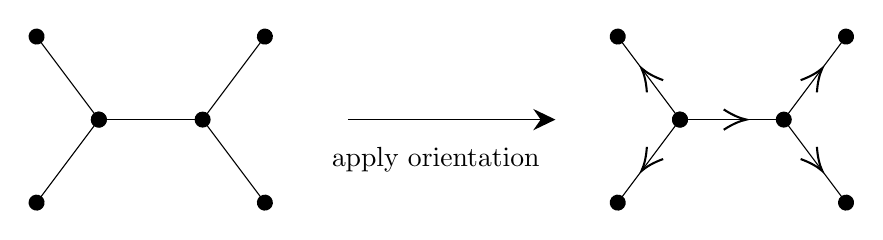
\begin{tikzpicture}[x=0.75pt,y=0.75pt,yscale=-1,xscale=1]
%uncomment if require: \path (0,111); %set diagram left start at 0, and has height of 111

%Straight Lines [id:da741919041298036] 
\draw    (40,50) -- (10,90) ;
\draw [shift={(10,90)}, rotate = 126.87] [color={rgb, 255:red, 0; green, 0; blue, 0 }  ][fill={rgb, 255:red, 0; green, 0; blue, 0 }  ][line width=0.75]      (0, 0) circle [x radius= 3.35, y radius= 3.35]   ;
\draw [shift={(40,50)}, rotate = 126.87] [color={rgb, 255:red, 0; green, 0; blue, 0 }  ][fill={rgb, 255:red, 0; green, 0; blue, 0 }  ][line width=0.75]      (0, 0) circle [x radius= 3.35, y radius= 3.35]   ;
%Straight Lines [id:da47409531598256205] 
\draw    (40,50) -- (10,10) ;
\draw [shift={(10,10)}, rotate = 233.13] [color={rgb, 255:red, 0; green, 0; blue, 0 }  ][fill={rgb, 255:red, 0; green, 0; blue, 0 }  ][line width=0.75]      (0, 0) circle [x radius= 3.35, y radius= 3.35]   ;
%Straight Lines [id:da2399175289181944] 
\draw    (90,50) -- (120,90) ;
\draw [shift={(120,90)}, rotate = 53.13] [color={rgb, 255:red, 0; green, 0; blue, 0 }  ][fill={rgb, 255:red, 0; green, 0; blue, 0 }  ][line width=0.75]      (0, 0) circle [x radius= 3.35, y radius= 3.35]   ;
%Straight Lines [id:da483679229546244] 
\draw    (90,50) -- (40,50) ;
\draw [shift={(40,50)}, rotate = 180] [color={rgb, 255:red, 0; green, 0; blue, 0 }  ][fill={rgb, 255:red, 0; green, 0; blue, 0 }  ][line width=0.75]      (0, 0) circle [x radius= 3.35, y radius= 3.35]   ;
\draw [shift={(90,50)}, rotate = 180] [color={rgb, 255:red, 0; green, 0; blue, 0 }  ][fill={rgb, 255:red, 0; green, 0; blue, 0 }  ][line width=0.75]      (0, 0) circle [x radius= 3.35, y radius= 3.35]   ;
%Straight Lines [id:da6663059195826004] 
\draw    (120,10) -- (90,50) ;
\draw [shift={(120,10)}, rotate = 126.87] [color={rgb, 255:red, 0; green, 0; blue, 0 }  ][fill={rgb, 255:red, 0; green, 0; blue, 0 }  ][line width=0.75]      (0, 0) circle [x radius= 3.35, y radius= 3.35]   ;
%Straight Lines [id:da7084400491516926] 
\draw    (320,50) -- (290,90) ;
\draw [shift={(290,90)}, rotate = 126.87] [color={rgb, 255:red, 0; green, 0; blue, 0 }  ][fill={rgb, 255:red, 0; green, 0; blue, 0 }  ][line width=0.75]      (0, 0) circle [x radius= 3.35, y radius= 3.35]   ;
\draw [shift={(301.4,74.8)}, rotate = 306.87] [color={rgb, 255:red, 0; green, 0; blue, 0 }  ][line width=0.75]    (10.93,-4.9) .. controls (6.95,-2.3) and (3.31,-0.67) .. (0,0) .. controls (3.31,0.67) and (6.95,2.3) .. (10.93,4.9)   ;
\draw [shift={(320,50)}, rotate = 126.87] [color={rgb, 255:red, 0; green, 0; blue, 0 }  ][fill={rgb, 255:red, 0; green, 0; blue, 0 }  ][line width=0.75]      (0, 0) circle [x radius= 3.35, y radius= 3.35]   ;
%Straight Lines [id:da21676438064922232] 
\draw    (320,50) -- (290,10) ;
\draw [shift={(290,10)}, rotate = 233.13] [color={rgb, 255:red, 0; green, 0; blue, 0 }  ][fill={rgb, 255:red, 0; green, 0; blue, 0 }  ][line width=0.75]      (0, 0) circle [x radius= 3.35, y radius= 3.35]   ;
\draw [shift={(301.4,25.2)}, rotate = 53.13] [color={rgb, 255:red, 0; green, 0; blue, 0 }  ][line width=0.75]    (10.93,-4.9) .. controls (6.95,-2.3) and (3.31,-0.67) .. (0,0) .. controls (3.31,0.67) and (6.95,2.3) .. (10.93,4.9)   ;
%Straight Lines [id:da40569083986374777] 
\draw    (370,50) -- (400,90) ;
\draw [shift={(400,90)}, rotate = 53.13] [color={rgb, 255:red, 0; green, 0; blue, 0 }  ][fill={rgb, 255:red, 0; green, 0; blue, 0 }  ][line width=0.75]      (0, 0) circle [x radius= 3.35, y radius= 3.35]   ;
\draw [shift={(388.6,74.8)}, rotate = 233.13] [color={rgb, 255:red, 0; green, 0; blue, 0 }  ][line width=0.75]    (10.93,-4.9) .. controls (6.95,-2.3) and (3.31,-0.67) .. (0,0) .. controls (3.31,0.67) and (6.95,2.3) .. (10.93,4.9)   ;
%Straight Lines [id:da7723467199596994] 
\draw    (370,50) -- (320,50) ;
\draw [shift={(320,50)}, rotate = 180] [color={rgb, 255:red, 0; green, 0; blue, 0 }  ][fill={rgb, 255:red, 0; green, 0; blue, 0 }  ][line width=0.75]      (0, 0) circle [x radius= 3.35, y radius= 3.35]   ;
\draw [shift={(352,50)}, rotate = 180] [color={rgb, 255:red, 0; green, 0; blue, 0 }  ][line width=0.75]    (10.93,-4.9) .. controls (6.95,-2.3) and (3.31,-0.67) .. (0,0) .. controls (3.31,0.67) and (6.95,2.3) .. (10.93,4.9)   ;
\draw [shift={(370,50)}, rotate = 180] [color={rgb, 255:red, 0; green, 0; blue, 0 }  ][fill={rgb, 255:red, 0; green, 0; blue, 0 }  ][line width=0.75]      (0, 0) circle [x radius= 3.35, y radius= 3.35]   ;
%Straight Lines [id:da9015362240911622] 
\draw    (370,50) -- (400,10) ;
\draw [shift={(400,10)}, rotate = 306.87] [color={rgb, 255:red, 0; green, 0; blue, 0 }  ][fill={rgb, 255:red, 0; green, 0; blue, 0 }  ][line width=0.75]      (0, 0) circle [x radius= 3.35, y radius= 3.35]   ;
\draw [shift={(388.6,25.2)}, rotate = 126.87] [color={rgb, 255:red, 0; green, 0; blue, 0 }  ][line width=0.75]    (10.93,-4.9) .. controls (6.95,-2.3) and (3.31,-0.67) .. (0,0) .. controls (3.31,0.67) and (6.95,2.3) .. (10.93,4.9)   ;
%Straight Lines [id:da28552551016148775] 
\draw    (160,50) -- (257,50) ;
\draw [shift={(260,50)}, rotate = 180] [fill={rgb, 255:red, 0; green, 0; blue, 0 }  ][line width=0.08]  [draw opacity=0] (10.72,-5.15) -- (0,0) -- (10.72,5.15) -- (7.12,0) -- cycle    ;

% Text Node
\draw (151,62) node [anchor=north west][inner sep=0.75pt]   [align=left] {apply orientation};


\end{tikzpicture}


        \caption{Applying the orientation in the case of \(n=4\). There is only one possible graph.}
        \label{fig:apply_orient}
    \end{figure}
    Next we consider possible orientations for the edges of the degree \(3\) vertices. Starting at a vertex with two outgoing edges, which are attached to two degree \(1\) vertices, edges are chosen for the degree \(3\) vertices in an ordered way, edges must be oriented so they form consecutive strings of \(+1\) or \(-1\), for example, for the graph in figure (\ref{fig:apply_internal}), relative to the starting vertex, the orientations:
    \[ \{ +1, +1 , +1\} ,\; \{ +1, +1 ,-1  \}, \; \{+1,-1,-1\}, \]
    are allowed, while 
    \[ \{ +1,-1,+1\},\]
    is not. This effectively generates a unique internal vertex in the graph, that all internal edges can be traversed to unambiguously. For more complicated graphs this means creating a vertex that acts as a sink. A sink is a vertex that all (internal) paths, following the orientation of the edges, lead to for example (\ref{fig:apply_internal}).
    \begin{figure}[htb]
        \centering
        

\tikzset{every picture/.style={line width=0.75pt}} %set default line width to 0.75pt        

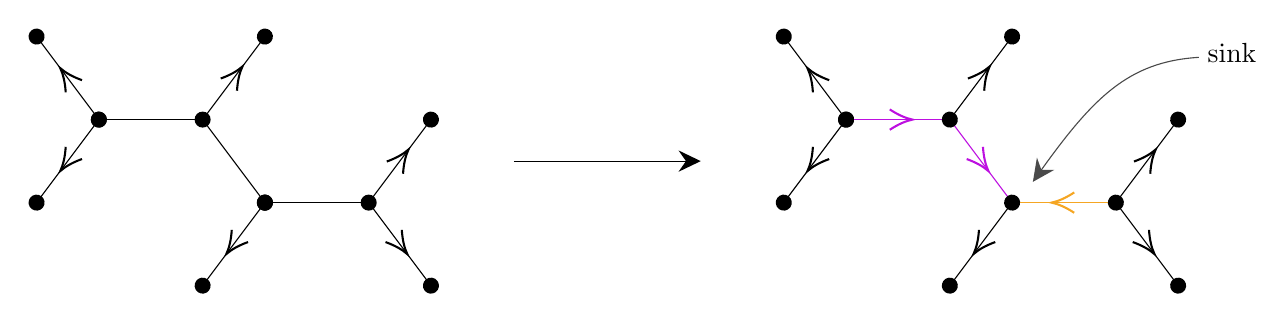
\begin{tikzpicture}[x=0.75pt,y=0.75pt,yscale=-1,xscale=1]
%uncomment if require: \path (0,151); %set diagram left start at 0, and has height of 151

%Straight Lines [id:da22627610725586034] 
\draw [color={rgb, 255:red, 189; green, 16; blue, 224 }  ,draw opacity=1 ]   (450,50) -- (400,50) ;
\draw [shift={(432,50)}, rotate = 180] [color={rgb, 255:red, 189; green, 16; blue, 224 }  ,draw opacity=1 ][line width=0.75]    (10.93,-4.9) .. controls (6.95,-2.3) and (3.31,-0.67) .. (0,0) .. controls (3.31,0.67) and (6.95,2.3) .. (10.93,4.9)   ;
%Straight Lines [id:da041653782173061815] 
\draw    (40,50) -- (10,90) ;
\draw [shift={(10,90)}, rotate = 126.87] [color={rgb, 255:red, 0; green, 0; blue, 0 }  ][fill={rgb, 255:red, 0; green, 0; blue, 0 }  ][line width=0.75]      (0, 0) circle [x radius= 3.35, y radius= 3.35]   ;
\draw [shift={(21.4,74.8)}, rotate = 306.87] [color={rgb, 255:red, 0; green, 0; blue, 0 }  ][line width=0.75]    (10.93,-4.9) .. controls (6.95,-2.3) and (3.31,-0.67) .. (0,0) .. controls (3.31,0.67) and (6.95,2.3) .. (10.93,4.9)   ;
\draw [shift={(40,50)}, rotate = 126.87] [color={rgb, 255:red, 0; green, 0; blue, 0 }  ][fill={rgb, 255:red, 0; green, 0; blue, 0 }  ][line width=0.75]      (0, 0) circle [x radius= 3.35, y radius= 3.35]   ;
%Straight Lines [id:da07326718492135587] 
\draw    (40,50) -- (10,10) ;
\draw [shift={(10,10)}, rotate = 233.13] [color={rgb, 255:red, 0; green, 0; blue, 0 }  ][fill={rgb, 255:red, 0; green, 0; blue, 0 }  ][line width=0.75]      (0, 0) circle [x radius= 3.35, y radius= 3.35]   ;
\draw [shift={(21.4,25.2)}, rotate = 53.13] [color={rgb, 255:red, 0; green, 0; blue, 0 }  ][line width=0.75]    (10.93,-4.9) .. controls (6.95,-2.3) and (3.31,-0.67) .. (0,0) .. controls (3.31,0.67) and (6.95,2.3) .. (10.93,4.9)   ;
%Straight Lines [id:da7839214017358417] 
\draw    (90,50) -- (120,90) ;
\draw [shift={(120,90)}, rotate = 53.13] [color={rgb, 255:red, 0; green, 0; blue, 0 }  ][fill={rgb, 255:red, 0; green, 0; blue, 0 }  ][line width=0.75]      (0, 0) circle [x radius= 3.35, y radius= 3.35]   ;
%Straight Lines [id:da14376202126053506] 
\draw    (90,50) -- (40,50) ;
\draw [shift={(40,50)}, rotate = 180] [color={rgb, 255:red, 0; green, 0; blue, 0 }  ][fill={rgb, 255:red, 0; green, 0; blue, 0 }  ][line width=0.75]      (0, 0) circle [x radius= 3.35, y radius= 3.35]   ;
\draw [shift={(90,50)}, rotate = 180] [color={rgb, 255:red, 0; green, 0; blue, 0 }  ][fill={rgb, 255:red, 0; green, 0; blue, 0 }  ][line width=0.75]      (0, 0) circle [x radius= 3.35, y radius= 3.35]   ;
%Straight Lines [id:da7008688072010646] 
\draw    (120,10) -- (90,50) ;
\draw [shift={(109.2,24.4)}, rotate = 126.87] [color={rgb, 255:red, 0; green, 0; blue, 0 }  ][line width=0.75]    (10.93,-4.9) .. controls (6.95,-2.3) and (3.31,-0.67) .. (0,0) .. controls (3.31,0.67) and (6.95,2.3) .. (10.93,4.9)   ;
\draw [shift={(120,10)}, rotate = 126.87] [color={rgb, 255:red, 0; green, 0; blue, 0 }  ][fill={rgb, 255:red, 0; green, 0; blue, 0 }  ][line width=0.75]      (0, 0) circle [x radius= 3.35, y radius= 3.35]   ;
%Straight Lines [id:da359668980650211] 
\draw    (170,90) -- (120,90) ;
\draw [shift={(120,90)}, rotate = 180] [color={rgb, 255:red, 0; green, 0; blue, 0 }  ][fill={rgb, 255:red, 0; green, 0; blue, 0 }  ][line width=0.75]      (0, 0) circle [x radius= 3.35, y radius= 3.35]   ;
\draw [shift={(170,90)}, rotate = 180] [color={rgb, 255:red, 0; green, 0; blue, 0 }  ][fill={rgb, 255:red, 0; green, 0; blue, 0 }  ][line width=0.75]      (0, 0) circle [x radius= 3.35, y radius= 3.35]   ;
%Straight Lines [id:da5577770273154145] 
\draw    (120,90) -- (90,130) ;
\draw [shift={(90,130)}, rotate = 126.87] [color={rgb, 255:red, 0; green, 0; blue, 0 }  ][fill={rgb, 255:red, 0; green, 0; blue, 0 }  ][line width=0.75]      (0, 0) circle [x radius= 3.35, y radius= 3.35]   ;
\draw [shift={(101.4,114.8)}, rotate = 306.87] [color={rgb, 255:red, 0; green, 0; blue, 0 }  ][line width=0.75]    (10.93,-4.9) .. controls (6.95,-2.3) and (3.31,-0.67) .. (0,0) .. controls (3.31,0.67) and (6.95,2.3) .. (10.93,4.9)   ;
\draw [shift={(120,90)}, rotate = 126.87] [color={rgb, 255:red, 0; green, 0; blue, 0 }  ][fill={rgb, 255:red, 0; green, 0; blue, 0 }  ][line width=0.75]      (0, 0) circle [x radius= 3.35, y radius= 3.35]   ;
%Straight Lines [id:da21435000458697373] 
\draw    (200,50) -- (170,90) ;
\draw [shift={(189.2,64.4)}, rotate = 126.87] [color={rgb, 255:red, 0; green, 0; blue, 0 }  ][line width=0.75]    (10.93,-4.9) .. controls (6.95,-2.3) and (3.31,-0.67) .. (0,0) .. controls (3.31,0.67) and (6.95,2.3) .. (10.93,4.9)   ;
\draw [shift={(200,50)}, rotate = 126.87] [color={rgb, 255:red, 0; green, 0; blue, 0 }  ][fill={rgb, 255:red, 0; green, 0; blue, 0 }  ][line width=0.75]      (0, 0) circle [x radius= 3.35, y radius= 3.35]   ;
%Straight Lines [id:da6194639262307314] 
\draw    (170,90) -- (200,130) ;
\draw [shift={(200,130)}, rotate = 53.13] [color={rgb, 255:red, 0; green, 0; blue, 0 }  ][fill={rgb, 255:red, 0; green, 0; blue, 0 }  ][line width=0.75]      (0, 0) circle [x radius= 3.35, y radius= 3.35]   ;
\draw [shift={(188.6,114.8)}, rotate = 233.13] [color={rgb, 255:red, 0; green, 0; blue, 0 }  ][line width=0.75]    (10.93,-4.9) .. controls (6.95,-2.3) and (3.31,-0.67) .. (0,0) .. controls (3.31,0.67) and (6.95,2.3) .. (10.93,4.9)   ;
%Straight Lines [id:da9011665660368904] 
\draw    (240,70) -- (327,70) ;
\draw [shift={(330,70)}, rotate = 180] [fill={rgb, 255:red, 0; green, 0; blue, 0 }  ][line width=0.08]  [draw opacity=0] (10.72,-5.15) -- (0,0) -- (10.72,5.15) -- (7.12,0) -- cycle    ;
%Straight Lines [id:da6450639046565149] 
\draw    (400,50) -- (370,90) ;
\draw [shift={(370,90)}, rotate = 126.87] [color={rgb, 255:red, 0; green, 0; blue, 0 }  ][fill={rgb, 255:red, 0; green, 0; blue, 0 }  ][line width=0.75]      (0, 0) circle [x radius= 3.35, y radius= 3.35]   ;
\draw [shift={(381.4,74.8)}, rotate = 306.87] [color={rgb, 255:red, 0; green, 0; blue, 0 }  ][line width=0.75]    (10.93,-4.9) .. controls (6.95,-2.3) and (3.31,-0.67) .. (0,0) .. controls (3.31,0.67) and (6.95,2.3) .. (10.93,4.9)   ;
\draw [shift={(400,50)}, rotate = 126.87] [color={rgb, 255:red, 0; green, 0; blue, 0 }  ][fill={rgb, 255:red, 0; green, 0; blue, 0 }  ][line width=0.75]      (0, 0) circle [x radius= 3.35, y radius= 3.35]   ;
%Straight Lines [id:da8590739970406319] 
\draw    (400,50) -- (370,10) ;
\draw [shift={(370,10)}, rotate = 233.13] [color={rgb, 255:red, 0; green, 0; blue, 0 }  ][fill={rgb, 255:red, 0; green, 0; blue, 0 }  ][line width=0.75]      (0, 0) circle [x radius= 3.35, y radius= 3.35]   ;
\draw [shift={(381.4,25.2)}, rotate = 53.13] [color={rgb, 255:red, 0; green, 0; blue, 0 }  ][line width=0.75]    (10.93,-4.9) .. controls (6.95,-2.3) and (3.31,-0.67) .. (0,0) .. controls (3.31,0.67) and (6.95,2.3) .. (10.93,4.9)   ;
\draw [shift={(400,50)}, rotate = 233.13] [color={rgb, 255:red, 0; green, 0; blue, 0 }  ][fill={rgb, 255:red, 0; green, 0; blue, 0 }  ][line width=0.75]      (0, 0) circle [x radius= 3.35, y radius= 3.35]   ;
%Straight Lines [id:da07942613501626583] 
\draw [color={rgb, 255:red, 189; green, 16; blue, 224 }  ,draw opacity=1 ]   (450,50) -- (480,90) ;
\draw [shift={(468.6,74.8)}, rotate = 233.13] [color={rgb, 255:red, 189; green, 16; blue, 224 }  ,draw opacity=1 ][line width=0.75]    (10.93,-4.9) .. controls (6.95,-2.3) and (3.31,-0.67) .. (0,0) .. controls (3.31,0.67) and (6.95,2.3) .. (10.93,4.9)   ;
%Straight Lines [id:da3697972639758368] 
\draw    (480,10) -- (450,50) ;
\draw [shift={(450,50)}, rotate = 126.87] [color={rgb, 255:red, 0; green, 0; blue, 0 }  ][fill={rgb, 255:red, 0; green, 0; blue, 0 }  ][line width=0.75]      (0, 0) circle [x radius= 3.35, y radius= 3.35]   ;
\draw [shift={(469.2,24.4)}, rotate = 126.87] [color={rgb, 255:red, 0; green, 0; blue, 0 }  ][line width=0.75]    (10.93,-4.9) .. controls (6.95,-2.3) and (3.31,-0.67) .. (0,0) .. controls (3.31,0.67) and (6.95,2.3) .. (10.93,4.9)   ;
\draw [shift={(480,10)}, rotate = 126.87] [color={rgb, 255:red, 0; green, 0; blue, 0 }  ][fill={rgb, 255:red, 0; green, 0; blue, 0 }  ][line width=0.75]      (0, 0) circle [x radius= 3.35, y radius= 3.35]   ;
%Straight Lines [id:da8337199770042564] 
\draw [color={rgb, 255:red, 245; green, 166; blue, 35 }  ,draw opacity=1 ][fill={rgb, 255:red, 245; green, 166; blue, 35 }  ,fill opacity=1 ]   (530,90) -- (480,90) ;
\draw [shift={(499,90)}, rotate = 360] [color={rgb, 255:red, 245; green, 166; blue, 35 }  ,draw opacity=1 ][line width=0.75]    (10.93,-4.9) .. controls (6.95,-2.3) and (3.31,-0.67) .. (0,0) .. controls (3.31,0.67) and (6.95,2.3) .. (10.93,4.9)   ;
%Straight Lines [id:da7264994944566067] 
\draw [fill={rgb, 255:red, 245; green, 166; blue, 35 }  ,fill opacity=1 ]   (480,90) -- (450,130) ;
\draw [shift={(450,130)}, rotate = 126.87] [color={rgb, 255:red, 0; green, 0; blue, 0 }  ][fill={rgb, 255:red, 0; green, 0; blue, 0 }  ][line width=0.75]      (0, 0) circle [x radius= 3.35, y radius= 3.35]   ;
\draw [shift={(461.4,114.8)}, rotate = 306.87] [color={rgb, 255:red, 0; green, 0; blue, 0 }  ][line width=0.75]    (10.93,-4.9) .. controls (6.95,-2.3) and (3.31,-0.67) .. (0,0) .. controls (3.31,0.67) and (6.95,2.3) .. (10.93,4.9)   ;
\draw [shift={(480,90)}, rotate = 126.87] [color={rgb, 255:red, 0; green, 0; blue, 0 }  ][fill={rgb, 255:red, 0; green, 0; blue, 0 }  ][line width=0.75]      (0, 0) circle [x radius= 3.35, y radius= 3.35]   ;
%Straight Lines [id:da8360809556285602] 
\draw    (560,50) -- (530,90) ;
\draw [shift={(530,90)}, rotate = 126.87] [color={rgb, 255:red, 0; green, 0; blue, 0 }  ][fill={rgb, 255:red, 0; green, 0; blue, 0 }  ][line width=0.75]      (0, 0) circle [x radius= 3.35, y radius= 3.35]   ;
\draw [shift={(549.2,64.4)}, rotate = 126.87] [color={rgb, 255:red, 0; green, 0; blue, 0 }  ][line width=0.75]    (10.93,-4.9) .. controls (6.95,-2.3) and (3.31,-0.67) .. (0,0) .. controls (3.31,0.67) and (6.95,2.3) .. (10.93,4.9)   ;
\draw [shift={(560,50)}, rotate = 126.87] [color={rgb, 255:red, 0; green, 0; blue, 0 }  ][fill={rgb, 255:red, 0; green, 0; blue, 0 }  ][line width=0.75]      (0, 0) circle [x radius= 3.35, y radius= 3.35]   ;
%Straight Lines [id:da574250525003525] 
\draw    (530,90) -- (560,130) ;
\draw [shift={(560,130)}, rotate = 53.13] [color={rgb, 255:red, 0; green, 0; blue, 0 }  ][fill={rgb, 255:red, 0; green, 0; blue, 0 }  ][line width=0.75]      (0, 0) circle [x radius= 3.35, y radius= 3.35]   ;
\draw [shift={(548.6,114.8)}, rotate = 233.13] [color={rgb, 255:red, 0; green, 0; blue, 0 }  ][line width=0.75]    (10.93,-4.9) .. controls (6.95,-2.3) and (3.31,-0.67) .. (0,0) .. controls (3.31,0.67) and (6.95,2.3) .. (10.93,4.9)   ;
%Curve Lines [id:da5997451992062178] 
\draw [color={rgb, 255:red, 74; green, 74; blue, 74 }  ,draw opacity=1 ]   (570,20) .. controls (535.75,22.11) and (518.74,39.44) .. (491.67,77.64) ;
\draw [shift={(490,80)}, rotate = 305.14] [fill={rgb, 255:red, 74; green, 74; blue, 74 }  ,fill opacity=1 ][line width=0.08]  [draw opacity=0] (10.72,-5.15) -- (0,0) -- (10.72,5.15) -- (7.12,0) -- cycle    ;

% Text Node
\draw (573,12) node [anchor=north west][inner sep=0.75pt]   [align=left] {sink};


\end{tikzpicture}

        \caption{Deciding on the internal orientation.}
        \label{fig:apply_internal}
    \end{figure}
    The degree \(1\) vertex adjacent to this sink becomes the root vertex. Flipping the direction of all the arrows from the root to the degree \(3\) vertices at the edges (only attached to two degree \(1\) vertices), we can see produces a binary tree. 
    
    The same idea will extend to generate the graphs in the quantum case, but instead graphs, we must consider multigraphs, where vertices are still all degree \(1\) or \(3\), but now can have two edges between vertices. Edges will still be labelled to create sinks, except for the presence of external tadpole like diagrams which decorate the edge of the graph.
    
    While these graphs are a binary tree, they have a special decoration, which will be important for deciding on how to label them with tensors to create the terms of \( u_{0}(x^{\sbt})\). Vertices with three outgoing edges will associated with \(a_{ijk}\) tensors, two outgoing and one incoming will be \(b_{ij}^k\) and finally one outgoing and two incoming a \(c_{i}^{jk}\). 
    
    %We define an outgoing edge to have sign \(1\), and define an incoming edge to have sign \(-1\). We define the \emph{energy} of a vertex, \( E\), to be the weighted sum:
    %\[ E(v) = \sum_{e \, \in \,\mathrm{edges}(v) } \mathrm{sign}(e). \] 
    %Finally every graph is given a \texttt{root} vertex. The \texttt{root} vertex is determined from the choice of orientation on the edges. The \texttt{root} is chosen to be a degree \(1\) vertex with the lowest energy. When \(n=3\) there is only one possible graph. When \(n=4\), the \texttt{root} vertex must necessarily be attached to a vertex with an incoming and an outgoing edge.
    
    
    %Every edge connecting to a degree \(1\) vertex must be the same orientation. Relative to the degree \(1\) vertex, all \(1\)-valent vertices must be attached to incoming edges. Apart from the \(n=3\) case, one vertex connected to the root vertex must have a single incomming edge.


    \subsubsection{Labelling graphs}
    
    To get the explicit monomials, for example \[ u_{0,5;i} = \left( c_i^{jk} a_{j r s } a_{k t u } + 4 b_{ir}^{k} b_{ks}^j a_{jtu} \right) x^r x^s x^t x^u, \]
    we label the graphs as described in the previous section, with tensors \( (a,b,c)\) and \(x\). For the term \( u_{0,n;i}\), for \( n \geq 3\), we consider the graphs in \(2n-2\) vertices where there are \(n\) degree \(1\) vertices, and \(n-2\), degree \(3\) vertices as described in the previous section. The free index \(i\) will correspond to the root vertex, and the other degree \(1\) vertices will represent an \(x^{\sbt}\).
    
    Vertices are labelled by tensors. A vertex with an outgoing edge will correspond to a lower index in the tensor labelling that vertex. An incoming edge corresponds to an upper index in the tensor labelling that vertex. 
    
    In terms of a vector space \(V\), lower indices corresponds to components of a tensor in \(V\), and an upper index corresponds to components in \(V^* \). An edge represents a tensor contraction.
    
    The graphs in the sum describing \( u_{0,n;i}\) will be labelled by the tensors \( (a_{\sbt,\sbt,\sbt},b_{\sbt,\sbt}^{\sbt}, c_{\sbt}^{\sbt,\sbt})\), and \(x^{\sbt}\).

    \begin{itemize}
        %\item All \(1\)-valent vertices must have an incoming edge (which represents pairing with an \(x^{\sbt}\)).
        %\item The \(1\)-valent vertex is labelled as the \texttt{root}, the rest with an \(x^{\sbt}\).
        %\item The graphs representing \(u_{0,n;i}\) have \(n\), degree \(1\) vertices and  \(n-2\), degree \(3\) vertices. 
        %\item All graphs are genus 0, \(g=0\), (no internal loops). A vertex is only connected directly to another vertex with a single edge. 
        \item All degree \(3\) vertices are labelled with one of the tensors \( (a_{\sbt,\sbt,\sbt},b_{\sbt,\sbt}^{\sbt}, c_{\sbt}^{\sbt,\sbt})\), where \( \sbt\) represents indices that need to inferred. 
        \item Label vertices with \(3\) outgoing edges with the tensor  \(a_{\sbt,\sbt,\sbt}\).
        \item  Label vertices with \(2\) outgoing and \(1\) incoming edges by the tensor \(2 \, b_{\sbt,\sbt}^{\sbt}\). 
        \item  Label vertices \(1\) outgoing and \(2\) incoming edges with the tensor \( c_{\sbt}^{\sbt,\sbt}\).
        %\item Diagrams are weighted, \(2\) outgoing propagators at a vertex contributes a weight of \(2\) to the diagram overall (alternatively we may just label as \(2 b_{ij}^k\)).
        %\item Let \(C_k\) denote the \(k\)-th Catalan number. There are \(C_{n-2}\) graphs with \(n\) \(1\)-valent vertices, counting weight, up to automorphism. 
        %\item All graphs are built up recursively from a graph with \(3\) \(1\)-valent vertices and \(1\) \(3\)-valent vertex, by adding on \(1\)-valent vertices. This represents starting with the term 
        %\( a_{ijk} \,x^j \,x^k \) in \( u_{0,n;i}(x)\). 
        \item We use Einstein summation convention and infer the labelling of the indices on the tensors. For tensors joined across an edge, which represents a contraction, an upper \({}^{\sbt}\) and a lower \({}_{\sbt}\) are fill with the same symbol. 
        \item The one unlabelled index on some tensor connecting to the \texttt{root} vertex is given the unique external index, for example denoted \(i\) if we are considering the graphs for \( u_{0,n;i}\). 
        \item Note that apart from \( u_{0,3;i}\), a vertex connected to the \texttt{root} is never labelled with \(a\).
    \end{itemize}
    So labelling every graph and then summing the labels together, gives \( u_{0,n;i}\).
    
    %Tensor contraction corresponds to a vertex with an outgoing edge connecting to another vertex which relatively gives it an incoming edge.
    
    %The first diagram corresponds to \(a_{ijk}\), so contributes a term of \( a_{ijk} x^i x^j x^k\) to \(S_0\). All other diagrams are built by adding vertices and propagators. 
    
    %There are two options for identifying these diagrams with a directed graph. First, as a graph with \(n-1\) vertices, \(n-2\) of them degree \(3\), and a special single vertex with degree \(n\).
    %
    %Overall each graph has \(2n-2\) vertices, \(n\) with degree \(1\), \(n-2\) with degree \(3\). 
    
    Recall that \(S_0(x^{\sbt})\) is defined as the primitive so \[ d S_0(x^{\sbt}) = u_{0;i}(x^{\sbt}) dx^i = \sum_{n \geq 3} u_{0,n;i}(x^{\sbt}) dx^i.\] 
    \(S_0\) is found by the previous labelling algorithm for \(u_{0,i}\), but instead now labelling the root vertex with an \(x^i\), and then multiplying by \(1/n\).
    \begin{ex}
    In the case of the conic, \(-y+a\,x^2 + 2 \,b \,x\, y + c\, y^2\), \( \dim(V)=1\),
    \[ S_0(x)= \frac{1}{3} a\, x^3 + \frac{1}{4}(2\, b\, a) \,x^4 + \frac{1}{5}( c \,a^2 + 4 \,b^2\, a)\,x^5 + \dots. \]
    \end{ex} 

    %Then 
    %\[ S_0(x^{\sbt}) = \sum_{n} \frac{R(\text{diagram}, x^{\sbt})}{|\text{Aut}(\text{diagram})|} \]   
    
   

    %\subsection{Casimir}
    %The \( H_i\) determine a Lie algebra with structure constants \( g_{ij}^k\). Denote \( [,]_{\mathfrak{g}}\) the Lie bracket determined by the \(H_i\) (but note is still computed via the Poisson bracket).
        
    %From the quadratic polynomials \( H_i\) we construct a \emph{Casimir}: \( \mathcal{H}(y_{\sbt},x^{\sbt}) : \mathcal{O}(W)\). 
    %Potential \( \mathcal{H}\) take the form \( \mathcal{H}(x^{\sbt},y_{\sbt}) = T(y_{\sbt}) + V(x^{\sbt})\), 
    
    %\( \mathcal{H}\) must satisfy the property that, for all \(i \), \( [ \mathcal{H}, H_i]_{\mathfrak{g}} = 0\).
    %One solution is given by
    %\begin{align*}
    %\mathcal{H} &= \int_0^1 d\lambda\, H_k(\lambda x^{\sbt}, \lambda y_{\sbt}) x^k + \lambda y_k x^k \\
    %            &= \frac{1}{3} \left( a_{ijk}x^{i}x^jx^k + 2  b_{ij}^k x^i x^j y_k +  c_{i}^{jk} x^i y_j y_k  \right)
    %\end{align*}
    %Now define a map 
    %\( (y_{\sbt}, x^{\sbt} ) \rightarrow ( x_{\sbt}, u^{\sbt}), \) where \( y_{i} \rightarrow  (x^j)^* = x_j\),
    %So    
    %\begin{align*}
    %\mathcal{L}(x_{\sbt},u^{\sbt}) &=  -\mathcal{H}(y_{\sbt} ,x^{\sbt}) + y_{i}  u^{j}|_{y\rightarrow x, x\rightarrow u} \\
    %&= a_{ijk} u^i u^j u^k + 2 b_{ij}^k u^i u^j x_k + c_{i}^{jk} u^i x_j x_k + x_i u^i
    %\end{align*}
    %Now consider 
    %\[ Z = \int D x_{\sbt} \exp \left( \frac{1}{\hslash} \int \left( a_{ijk} u^i u^j u^k + 2 b_{ij}^k u^i u^j x_k + c_{i}^{jk} u^i x_j x_k + x_i u^i  + J \right) \right) \] 
    
    %Set \(T(y_{\sbt}) = \sum_{n} T^{i_1, \dots i_n} y_{i_1} \dots y_{i_n}\).
    %The terms which are required to vanish non trivially are: 
    %\( \{ T^{i_1, \dots i_n} y_{i_1} \dots y_{i_n}, a_{ijk}x^j x^k \}\), and \(  2 \{ T^{i_1, \dots i_n} y_{i_1} \dots y_{i_n}, b_{ij}^k x^j y_k \} \).

    %Likewise set \( V(x_{\sbt}) = \sum_{n} V_{i_1, \dots i_n} x^{i_1} \dots x^{i_n}\).
    %So there are non trivial vanishing terms:
    %\( \{ V_{i_1, \dots i_n} x^{i_1} \dots x^{i_n}, c_{i}^{jk} y_j y_k \}\),  \(  2 \{ V_{i_1, \dots i_n} x^{i_1} \dots x^{i_n}, b_{ij}^k x^j y_k \} \) and \( - \{  V_{i_1, \dots i_n} x^{i_1} \dots x^{i_n}, y_i \}\).


    %\newpage 
    
    \iffalse 
    
    \subsection{Lie algebra structure}

    The Airy structure determines a Lie algebra. 
    
    In the Tate or the affine case, \( \mathcal{O}(W)\) has a maximal ideal \(\mathfrak{m} = \langle x^{\sbt}, y_{\sbt} \rangle\).  Denote \( L_i = -y_i \), the linearisation of \(H_i\). The (Zariski) tangent space of \( \cL\) at \(0\) is given by \(  T_0 \cL = \mathfrak{m}/(\langle L_i \rangle  + \mathfrak{m}^2) \cong L \cong \langle y_i \rangle  \ \). Further this gives \(\{x^i\}\) as coordinates on \(L\), and \(y_i\) can be identified with derivations \( \frac{\partial}{\partial x_i}\) on \( \cL\).

    The tangent space \( L \cong T_0\cL\) is equipped with the structure of a Lie algebra \( \mathfrak{g} = (L, [, ]_{\mathfrak{g}}) \) as follows. The constants \(g_{ij}^k\) from the closure of the Poisson bracket on \(I = \{ H_i\}\), determine the structure constants of \( \mathfrak{g}\). This gives a Lie bracket on \( L\) defined as \( [y_i,y_j]_{\mathfrak{g}} =g_{ij}^k y_k\). 

    
    We have the usual Lie algebra homomorphism between Hamiltonian vector fields and functions 
    
    On \(W\), for the function \(H_i\), define a Hamiltonian vector field:
    \[ X_{H_i} = \left( \frac{\partial H_i}{\partial y_j}, - \frac{\partial H_i}{\partial x^j} \right). \]

    \begin{align*}
    \frac{\partial H_i}{\partial y_j} &= - \delta_{ij} + 2 b_{im}^j x^m + 2 c_{i}^{j m} y_m \\
    -\frac{\partial H_i}{\partial x_j} &= -2 a_{ijm}x^m - 2 b_{ij}^m y_m
    \end{align*}
    Then the the corresponding Lie bracket of vector fields is given by:
    \[ [X_{H_i}, X_{H_j} ]_{\mathfrak{g}} = X_{\{H_i,H_j\}} = X_{g_{ij}^k H_k}. \]
    
    
    
    %The Hamiltonian vector fields define foliations.
    
    %Picking a morphism \(x \rightarrow x(t_1, \dots ), y\rightarrow y(t_1, \dots)\), and solving the Hamiltonian equations in terms of \(t\) 
    %\begin{align*}
    %    \dot{x}_j &= \sum_i \frac{\partial H_i}{\partial y_j} \\
    %    \dot{y}_j &= -\sum_i \frac{\partial H_i}{\partial x_j}
    %\end{align*}
    %gives explicit parameterisations of level curves on  \( \mathcal{L}\). 
    %\begin{align*}
    %    \left( \begin{array}{c}
    %         x \\
    %         y 
    %    \end{array}\right) &= \exp \left(2 t \left(   \begin{array}{cc}
    %         b & c  \\
    %         -a & -b  
    %    \end{array} \right)\right) \cdot \left( \begin{array}{c}
    %         x_0  \\
    %         y_0  
    %    \end{array} \right) + \int_0^t du \exp \left(2 (t-u) \left( \begin{array}{cc}
    %         b & c  \\
    %         -a & -b  
    %    \end{array} 
    %    \right)
    %    \right) \cdot \left( \begin{array}{c}
    %         \mathbf{1}  \\
    %         0  
    %    \end{array}\right)
    %\end{align*}
    %It is possible to check that these satisfy the equations \(H_i = 0\).
    
    On \( \mathbb{L}\), with coordinates \(\{x_i\}\), there are vector fields, or derivations, given by
    \[ \xi_i=\frac{\partial}{\partial x^i}+ f_{ij}\frac{\partial}{\partial y^j} \] 
    such that \( d H_i ( \xi_i ) = 0\).
    
    
    
    
    %The motivation is to treat \( \mathbb{C}\lParen z \rParen\) as an algebraic-geometric object over \( \Spec( \mathbb{C})\), so treating \( \mathbb{C}\lParen z \rParen\) as a scheme .
    %The \(H_i\) form a \emph{Poisson ideal}, and then this defines a quadratic \emph{Lagrangian} subscheme
    %\[ \mathcal{L} \simeq \Spf \left( \frac{\mathbf{k}\lBrack x^{\bullet},y_\bullet \rBrack}{\langle H_i \rangle} \right)  \] 
    %which has a tangent space \( L \simeq V^*\). In finite dimensions this a subvariety or a Lagrangian submanifold.
    
    %\( \mathcal{L} \) can be represented by a formal power series, \( S_0(x^\bullet)\). Computing the root, \( H_i(x^\bullet,y_\bullet) =0\) as a function \(y_i(x^\bullet) = S_{0,i}(x^\bullet)\), can be treated as a fixed-point iteration problem.
    
    %Define the fixed point iteration 
    %\begin{align*} 
    %    S^{[n]}_{0,i} &= a_{ijk} x^j x^k + 2 b_{ij}^k x^j S^{[n-1]}_{0,k} + c_i^{jk} S^{[n-1]}_{0,j} S^{[n-1]}_{0,k}, \\
    %    S^{[3]}_{0,i} & = a_{ijk} x^j x^k.
    %\end{align*}
    %and consider \(\mathcal{S}_{0,\infty;i} \). The tensor \( S_{0,n;i} \) is the component with \({n-1}\) degree \(x^{\bullet}\) terms in \(\mathcal{S}_{0,\infty;i} \).

    %\begin{rem} An Airy structure is a functor on an Artin algebra.
    %\end{rem}

    \fi 
    
    \section{Quantum Airy structures}
    
    Let \( (\mathcal{O}_W \lBrack \hslash \rBrack ,\star)\) be the deformation quantisation of \( (W,\mathcal{O}_W)\).  The idea is to find a \( \mathcal{O}_W\lBrack \hslash \rBrack\)-module, such that under the quotient map \( \hslash \rightarrow 0\), gives a module supported on a Lagrangian \( \cL\).  

    \subsection{Affine case}

    Consider a finite dimensional polynomial ring in \(2n\) variables \( \mathcal{O}(W)= \mathbf{k}[x^i, y_j]\), with a Poisson bracket defined on the generators by \( \{ y_i, x^j \} = \delta_{i}^j, \{ x^i, x^j\} = \{y_i,y_j\} = 0\). Note in infinite dimensions, this ring has additional structure, lemma (\ref{lem:coordring}).
    
    We consider a deformation quantisation of \( \mathcal{O}(W)\), given by  \((\mathcal{O}(W)\lBrack \hslash \rBrack, \star ) \), where \( \star\) is the usual Moyal star product, definition (\ref{defn:star_prod_pois}). On the generators we have the products:
    \begin{align*}
         x^i \star x^j &= x^i x^j \\
         x^i \star y_j &= x^i y_j - \frac{\hslash}{2} \delta_{j}^i\\ 
         y_j \star x^i &= x^i y_j + \frac{\hslash}{2} \delta_{j}^i \\ 
         y_i \star y_j &= y_i y_j
    \end{align*}
    where terms like \(x^i y_j\) are a new function in \(\mathcal{O}(W)\lBrack \hslash \rBrack\), not a product.
    
    %In finite dimensions, the Moyal product would be evaluated over \( 4 n\) variables (note temporarily repeated indices are not summed):
    %\begin{align*}
    %    x^i \star x^j &= \frac{1}{Z} \int D q^{\sbt} D q'^{\sbt} 
    %    D p_{\sbt} D p'_{\sbt}\, q^i q'^j \exp \left(-\frac{1}{2 \hslash} (p_i x^i - p'_j x^j + p_{\sbt} q^{\sbt} - p'_{\sbt} q'^{\sbt}  ) \right)\\
    %    &= \frac{1}{Z} \int Dq^i Dq'^j Dp_i Dp'_j q^i q^j \exp \left(-\frac{1}{2 \hslash} (p_i x^i - p'_j x^j + p_{i} q^{i} - p'_{j} q'^{j}  ) \right) \\
    %    &= x^i x^j+ \hslash
    %\end{align*}
    We now consider the deformation quantisation of a subvariety \( \mathcal{E}\) defined by an ideal \(I=  \langle H_i \in \mathcal{O}(W)\rangle \) of quadratic polynomials \( H_i\), and a corresponding dual \(\mathcal{O}_W \lBrack \hslash \rBrack\)-module.  Suppose in local coordinates suppose \(H_i \) take the form:
    \begin{align*}
            H_i =  -y_i + a_{ijk}\, x^i  x^j +   2  \,  b_{ij}^k  \, x^j y_k +  c_{i}^{jk} \, y_j  y_k.
    \end{align*}
    Necessarily any module of the form 
    \[ \mathcal{E}_{\hslash} = \mathcal{O}(W) \lBrack \hslash \rBrack /  \mathcal{O}(W) \lBrack \hslash \rBrack \cdot \langle H - \hslash J\rangle \]
    restricts to \( \mathcal{E}\) under the quotient map by \(\hslash\). Furthermore we are also interested in the dual \(\mathcal{O}_W \lBrack \hslash \rBrack\)-module 
    \[ \mathcal{E}_{\hslash}^{\vee} = \Hom( \mathcal{E}_{\hslash}, \mathcal{O}(W)\lBrack\hslash\rBrack) ,\]
    which encodes solutions to the equations 
    \[( H_i - \hslash J_i) \star w = 0.\]
    For now we consider the case where \( \hslash J_i \) are elements of \( \mathbf{k}\lBrack \hslash \rBrack\).
    
    To analyse this problem \( (\mathcal{O}_{W} \lBrack \hslash \rBrack, \star) \) is identified with a Weyl algebra \( \mathcal{W}_{\hslash}\), with an isomorphism \( \varphi :\mathcal{O}_{W} \lBrack \hslash \rBrack \rightarrow \mathcal{W}_{\hslash} \). On the generators \(\varphi( x_i) = x_i \) and \( \varphi(y_i) = \hslash\, \partial_i \). Furthermore, star products correspond to operator products:
    \begin{align*}
         \varphi(x^i \star x^j) &= x^i x^j \\
         \varphi(x^i \star y_j) &= \hslash x^i  \partial_j \\
         \varphi(y_j \star x^i) &= \hslash \partial_j ( x_j \cdot ) \\ 
        \varphi( y_i \star y_j) &= \hslash^2 \partial_i \partial_j  
    \end{align*}
    To find the image of a function, for example \(\varphi( x^i y_j)\), in the Weyl algebra, we have to use the definition of star product and try to work out which star products will give the desired term. For quadratic terms this is relatively simple, and follows from the definition immediately, for example:
    \[ x^i y_j = x_i \star y_j + \frac{\hslash}{2} \delta_{j}^i,\]
    so 
    \[ \varphi(x_i y_j ) = \varphi(y_j x^i) = \varphi\left(x^i \star y_j + \frac{\hslash}{2} \delta_{j}^i \right) = \hslash\, x^i \frac{\partial}{\partial x_j} + \frac{\hslash}{2} \delta_{j}^i.\] 
    \begin{rem}
    Note \(\partial_i \) can be identified with the vector field, or derivation, \( \frac{\partial}{\partial x^i}\) when \( \hslash \) is invertible.  
    \end{rem}
    So with the deformation quantisation procedure, there is no ambiguity of ordering, but there are clearly many modules corresponding to different choices of \(\hslash J\), which have the same classical limit. The map to the Weyl algebra however does introduce a constant term, but this is not a choice, it follows directly.
    
    So now we consider the image of \( \varphi((H_i-\hslash J_i) \star w) \), which is used to define an operator equation \((\widehat{H}_i - \hslash J_i) \psi = 0\).
    The image of the functions \(H_i\) under the isomorphism to the Weyl algebra are operators  \(\widehat{H}_i = \varphi(H_i) \):
    \[ \widehat{H}_i := \hslash\, \partial_i + a_{ijk} x^i x^j +   2 \hslash \,  b_{ij}^k  \, x^j \partial_k + \hslash^2 c_{i}^{jk} \partial_j \partial_k  + \hslash\, \widetilde{\varepsilon}_i + \hslash J_i,\] 
    where we must have 
    \[ \widetilde{\varepsilon}_i = b_{ij}^k \delta_{k}^j.\]
    This is consistent with quantisation presented in \cite{ks_airy}. 
    \begin{rem}
    The coefficients \( \widetilde{\varepsilon}_i\) give a tensor \( \widetilde{\varepsilon}: V\),
    \[ \widetilde{\varepsilon} = \widetilde{\varepsilon}_i x^i.  \]
    \end{rem}
    For a moment suppose the \(\widehat{H}_i\) and \(\mathcal{W}_{\hslash}\) exist independently of \( \mathcal{O}(W)\lBrack\hslash\rBrack\). Kontsevich and Soibelamn define an \emph{Airy structure} on \( \mathcal{W}_{\hslash} \) to be a choice of coefficients of \(\widehat{H}_i\), such that the \(\widehat{H}_i\) are closed under the Lie bracket: 
    \[ [\widehat{H}_i , \widehat{H}_j] = g_{ij}^k \widehat{H}_k.\]
    %Note that in this non-commutative case we do not consider there to be some non-commutative space unless we consider primitive ideals/primitive spectrums
    Returning back to the case where there is an isomorphism to a space \( \mathcal{O}(W)\lBrack \hslash \rBrack\), Kontsevich and Soibleman then define a \emph{quantum Airy structure} as constraints on a particular tensor \(  \varepsilon \in V\), or a collection of numbers \(\varepsilon_i : \mathbf{k}\), so there is a correspondence between the Poisson structure of \(H_i\) and \( \widehat{H}_i\), 
    \[ [\widehat{H}_i , \widehat{H}_j] \rightarrow \hslash \{ H_i , H_j \} + \hslash g_{ij}^k \varepsilon_k. \]
    In our case, this may put extra constraints on the choice of \(J_i\).
    
    %This generates a wavefunction supported on \( \mathcal{O}_{\hatL} \lBrack \hslash \rBrack\).

    
    \begin{defn}[quantum Airy structure, \cite{ks_airy}]
    \label{defn:airystructquant}
    A \emph{quantum Airy structure} is a collection of tensors satisfying
    \[ 2 \left( a_{jst} \, c_i^{st} - a_{ist} \, c_j^{st} \right) = g_{ij}^k \varepsilon_k.\]
    \end{defn}
    See appendix (\ref{appendix:quantum_airy}) for the explicit calculation of this constraint.
    
    Necessarily we must have
    \[ \varepsilon_i = \widetilde{\varepsilon}_i + J_i\]
    which means \(J_i\) must be chosen to satisfy:
    \[2 \left( a_{jst} \, c_i^{st} - a_{ist} \, c_j^{st} \right) = g_{ij}^k ( b_{k s }^{s} - J_k).\]
    
    \subsubsection{Quantisation in infinite dimensions and the trace of the \texorpdfstring{\(B\)}{B} tensor}
    
    We see that the trace of the \(B\) tensor \(b_{ij}^{j}\), is an obstruction to existence of quantisation in infinite dimensions. This is where a choice of topology or the method of extension to infinite dimensions becomes important.
    
    In the case where we take a pro-infinite, or limit of the \(n\), of the \(y^i\) per chapter (\ref{chapter:infalg}),
    this allows a potentially infinite combination of separate \(y^i\), for example:
    \[ y_1 + y_2 + y_3 + \dots, \]
    although note there are no infinite sums of powers of an individual \(y_i\). Simultaneously if there is an ind-infinite extension, or a colimit in \(n\) of the \(x^{\sbt}\), this still allows a pontentially infinite sum from \(b_{ij}^j\) because of the interaction with the \(y^{\sbt}\). 
    
    One solution is that \(b\) must only contain finitely many non zero terms. The other choice is that \(b_{ij}^j\) is a convergent series, in terms of partial sums. 
    
    %Taking the colimit of \(x^i\) terms gives a ring with infinite \(x^{\sbt}\) variables, but elements of the ring only contains terms with finite sums of \(x^{\sbt}\) variables, so an expression like \( b_{\sbt\, j}^{\sbt} x^j \) contains a finite sum of \(x^j\). 
    Another solution is using the idea of  \emph{renormalisation}. As we increase the number of \(x^i\) or \(y^i\) terms, although the sum \(b_{ij}^{j}\) may be growing, it is possible to adjust \(J_k\) accordingly, so the contribution from \(b_{ij}^j \) is cancelled in the operators \(\widehat{H}_i\).
    
    \begin{ex}
    For example suppose for some fixed \(i\), \(b_{ik}^k = 1 + 2 + 3 + \dots + n \). Then set \(J_{i} = n(n+1)/2\). Then as \(n \rightarrow \infty\), \( b_{ik}^k - J_{i} = 0\). Note that the constraints on the \(a\) and \(c\) tensors must also be satisfied.
    \end{ex}
    
    Of course this is also conditional on the constraints for \(a\) and \(c\), per definition (\ref{defn:airystructquant}). In chapter (\ref{chapter:Atensor}), is an example of this procedure. Overall, this suggests we should simply study the \emph{renormalised Hamiltonians}, were contributions of constants from quantisation have been cancelled out:
    \begin{ex}[Renormalised Hamiltonians]
    \label{defn:renormalised}
    \[ \widehat{H}_i := \hslash\, \partial_i + a_{ijk} x^i x^j +   2 \hslash \,  b_{ij}^k  \, x^j \partial_k + \hslash^2 c_{i}^{jk} \partial_j \partial_k  \] 
    \end{ex}
    Note that under the classical limit, these still reduce to the \(H_k\), so it counts as a valid deformation quantisation.
    
    This also motivates the definition of calling \( \varepsilon_i\) a \emph{tadpole diagram} when labelling some graphical expression. When solving the equations \( \widehat{H}_k \psi = 0\), in the form  \(\psi = \exp(S(x))\), where \(S(x)\) is a series in the coefficients \( (a,b,c,\varepsilon)\), \(x^{\sbt}\) and \(\hslash\), \( \varepsilon_i\) contributions are always identified with graphs, which can be separated into a piece labelled from \((a,b,c)\), and then a vertex with an extra self loop. 
    

    
    %\subsection{Lie algebra}
   
    %The  quantisation of a Poisson Lie algebra \( \mathfrak{g}\), with Poisson bracket \( \{,\}\), needs to give a Lie algebra of operators \(\widehat{H}_i\) with a Lie bracket. A necessary condition to do this, is that the second cohomology vanishes, \(H^2(\mathfrak{g}, \mathbf{k})=0\). This is a choice of central extension to \(\mathfrak{g}\) so the Lie algebra structure of the quantum and classical cases coincide to order \( \hslash\). A choice of extension is also equivalent to an element \( \varepsilon : V^* \), or numbers \( \varepsilon_i : \mathbf{k}\).
    

    

    \subsection{Wavefunctions}
    
    A quantum Airy structure encodes an object called a wavefunction \emph{supported} on \(\widehat{\cL} \). 
    As per the example of the conic in chapter (\ref{chapter:deformation}), we use the Weyl algebra representation and solve the operator equations on a formal completion. Let
    \[ \widehat{\mathcal{W}}_{\hslash} = \mathbf{k} \lBrack x^{\sbt}, \hslash \partial_{\sbt} \rBrack \lBrack \hslash \rBrack \] 
    denote the completed Weyl algebra (which corresponds to completion at point \((x,y)=(0,0)\). Then we consider:
    \[ \mathcal{S}_{\hslash} = \Hom\left( \widehat{\mathcal{W}}_{\hslash}/\widehat{\mathcal{W}}_{\hslash} \cdot \widehat \langle \widehat{H}_k - \hslash J_k \rangle , \widehat{\mathcal{W}}_{\hslash} \right), \]
    where 
    \[ \widehat{H}_i =  - \hslash \frac{\partial}{\partial x_i} + a_{ijk} x^j x^k + 2 b_{ij}^k \hslash x^j \frac{ \partial }{\partial x_k}+ \hslash^2 c_{i}^{jk} \frac{\partial^2}{\partial x_j \partial x_k} + \hslash \widetilde{\varepsilon}_i ,\]
    and \( \widehat{\varepsilon}_i = b_{ij}^j\) as before. The module \( \mathcal{S}_{\hslash}\) encodes the solutions to the equations \[ (\widehat{H}_k - \hslash J_k ) \psi_{\cL} = 0.\]
    \begin{prop}
    \( \mathcal{S}_{\hslash} \) is cyclic, hence generated by a single element \( \psi_{\cL} \).
    \end{prop}
    %Therefore this module is said to encode the solution to the \(\widehat{H}_i\) acting as operators on \( \mathbf{k}\lBrack x^{\bullet} \rBrack \lBrack \hslash  \rBrack \).
    From now on, we use a change of notation, and define
    \[ \varepsilon_k = \widetilde{\varepsilon}_k - J_k,\]
    and then redefine \( \widehat{H}_k \) to include these terms, be consistent with the notation in \cite{ks_airy}, so 
    \[ \widehat{H}_i =  - \hslash \frac{\partial}{\partial x_i} + a_{ijk} x^j x^k + 2 b_{ij}^k \hslash x^j \frac{ \partial }{\partial x_k}+ \hslash^2 c_{i}^{jk} \frac{\partial^2}{\partial x_j \partial x_k} + \hslash \, \varepsilon_i, \] 
    and consider the module \( \mathcal{W}_{\hslash} / \mathcal{W}_{\hslash} \cdot \widehat{H}_i \), and its dual.
    %If \( \mathcal{S}_{\hslash} \) as a \( \mathcal{W}_{\hslash} \)-module is cyclic and generated by \( \psi\) then it is isomorphic to \(\mathcal{E}_{\hslash}   / \mathrm{Ann}_{\mathcal{E}_{\hslash}} \psi \). Therefore we need to find the \( \psi\).
    
    %The zero class corresponds to non-zero elements after the action of \( \widehat{H}_{\bullet}\).
    
    %Given \(f,g \in \mathcal{W}\), define \(f \sim g \) if they can be represented as \( f = \widehat{H}_{\bullet} (\varphi)\) and \(g = \widehat{H}_{\bullet} (\vartheta)\).
    
    
    The \emph{wavefunction} \( \psi = \psi_{\cL} \),  is computed explicitly using the ansatz: 
    \[ \psi_{\cL}(x^{\sbt}) = \exp(S(x^{\bullet})),\]
    where
    \[ S(x^{\bullet}) = \sum_g \hslash^{g-1} S_g(x^{\bullet}),\]
    and solving the partial differential equations:
    \[ \widehat{H}_i \exp(S(x^{\bullet})) = 0. \] 
    Modulo \(\hslash \), \( \psi_{\mathbb{L} }\) is a function supported on \( \widehat{\mathbb{ L}} \), (formal neighbourhoods of \(\cL\)). In the next section we do this explicitly.
    
    
    \begin{rem}   This equation is understood from an algebraic perspective, a solution is a formal power series.
    \end{rem}
    
    %Individually \(S_g(x^{\bullet}) : \mathbf{k} \lBrack x^{\bullet}\rBrack\). 
    %\begin{thm}[existence]
    %\end{thm}
    \begin{ex} Consider the quantised conic:
    \[ \left( - \hslash \frac{\partial}{\partial x} + a x^2 + 2 b \hslash x \frac{ \partial }{\partial x}+ \hslash^2 c \frac{\partial^2}{\partial^2 x} + \hslash \, \varepsilon \right) \psi_{\mathbb{L}}(x)  = 0. \]
    The wavefunction is given by:
    \[ \psi_{\mathbb{L} }(x) = \exp \left( \frac{1}{\hslash} \int dx \, ( u_0(x)  + \hslash \, u_1(x) + \mathcal{O}(\hslash^2) ) \right), \]
    where integration is understood as formal integration.  Note this wavefunction is defined at the point \((x,y)=(0,0)\).
    \begin{itemize}
        \item  If \( (a,b,c,\varepsilon) = (1,1,1,0)\), then \( u_0(x)\) is as example \ref{example:conic_airy}, and
        \[u_1(x) =\frac{1 - \sqrt{1 -4x}}{1-4x}= 2 x + 10 x^2 + \cdots + \left(4^n - \frac{(2n)!}{(n!)^2}\right) x^n + \cdots,\]
        where \(u_1\) is the generating function for counting numbers of rooted two-face \(n\)-edge maps in the plane, (1-loop Feynman diagrams) \cite{feynmaps}. 
        %This is also the root of a polynomial:
        %\[ 4 x - 2 u_1 + 8 x u_1 + (1 - 4 x)^2 u_1^2 = 0.\]
        %Also note 
        %\[ u_1(x) = \frac{2 u_0(x)  x}{1 - 4 x}\]
    \end{itemize}
    \end{ex}
    % 
    % solving for u_0 = y, and multiplying by conjugate root gives : 1 - y + x y^2
    
    
    %\subsection{Factorisation}
    
    %Consider the conic, \(H=-y + a x^2 + b x y +c  y^2\), there is a ring morphism 
    %\[ \mathbf{k}\lBrack x ,y \rBrack /H \cong \mathbf{k} \lBrack x,y \rBrack /L_1 \times  \mathbf{k} \lBrack x,y\rBrack /L_2\]
    %where \(H=L_1 L_2\). However \( \widehat{H} \neq \widehat{L}_1 \cdot \widehat{L}_2\), 
    
    
    \section{Abstract topological recursion}
    \label{sec:abstract_top_rec}
    
    A result of Kontsevich and Soibelman \cite{ks_airy} is that the coefficients of \(S_{g,n}\) of \(S\) satisfy \emph{\hyperref[defn:abstracttr]{abstract topological recursion}}. Denote \(S_{g,n;i_1, \dots i_k} = \partial_{i_k} \dots \partial_{i_1} S_{g,n}\).
    
    \begin{defn}[Abstract topological recursion] 
    \label{defn:abstracttr}
    The recursive formula:
    \begin{align*}
        S_{g,n;i,i_1,\dots,i_{n-1}} =&  \, c^{jk}_i S_{g-1,n+1;j,k,i_1, \dots i_{n-1}} +  2 \sum_{\alpha = 1 }^{n-1} b^k_{i \, i_\alpha} S_{g,n-1;k i_{\{1,\dots n-1\}/\{\alpha\}}}  \\
        &+ \hspace{-10pt} \sum_{\substack{g_1 + g_2 = g \\ I_1 \sqcup I_2 = \{1, \dots, n-1\}} } \hspace{-10pt} c^{jk}_i S_{g_1, \# I_1 + 1; j}\, S_{g_2, \# I_2+1;k} , 
    \end{align*}
    is called \emph{abstract topological recursion}, for \(g=0,n>3\) and \(g>1,n\geq 0\).
    \end{defn}
    
    To see the definition, apply the \( \widehat{H}_i\) to \(\psi_{\cL} \)  and solve for \(0 \): 
    \begin{align*}
        & a_{ijk} x^j x^k + \sum_g \bigg( 2 \, \hslash\, b_{ik}^{j}\, \sum_n  S_{g,n;j} x^k + \\
        &\hslash^2 \, c_i^{jk}  \left(\sum_n S_{g,n;j,k} + \sum_n S_{g,n;j} S_{g,n;k} \right) - \hslash \, S_{g,n;i} + \hslash \,\varepsilon_i \bigg)  = 0.
    \end{align*} 
    Gathering like \(\mathcal{O}(\hslash^g)\) terms gives the formula from definition (\ref{defn:abstracttr}). The sum of \(g-1\) and \(g_1+g_2 = g\) terms is analogous to topological recursion. 


    \begin{corollary}
    \( S_{1,n} \) can be computed from \(S_{0,n}\) and \(\varepsilon\).
    \end{corollary}
    
    This just follows from the recursion directly.

    \begin{lem}[\cite{ks_airy}]
    The \( S_{g,n}\) are symmetric under permutations of \(x^i\).
    \end{lem}
    
    This was proven by Kontsevich and Soibelman and follows from the properties of the tensors \( A,B,C\).
    
    \begin{rem}
    Note this recursion has explicitly made a choice. A bit like the conic \( - y + x^2 + 2 x y + y^2\), and solving for \(y\) gives two possible choices for the square root, this series has made a similar choice, it corresponds to a completion at \((x,y)=(0,0)\). This is why the module is cyclic.
    \end{rem}
    %Instead of quantising the quadratic Hamiltonians, it is also possible to consider the linear operators given by quantising \( y = u_0\).

    Eynard Orantin topological recursion \cite{eynard_orantin}, can be seen as a particular specialisation of abstract topological recursion. With the right choice of \(V\), restricting to the odd \(H_i\) recovers topological recursion. The identification with the tensors in \(\widehat{\mathrm{Sym}}(V)\) proves the symmetry of \( \omega_{g,n}\).    

    
    Closure of the Poisson bracket gives rise to the symmetry of the multi differentials in ordinary topological recursion, as it can be considered a specialisation of abstract topological recursion.

    \subsection{Diagrams}
    The tensors \( S_{g,n}\) are treated in a very similar way to the \(S_{0,n}\) case. As before there are graphs labelled by \((a,b,c)\), but we need multi-graphs, which are graphs with multiple edges between nodes.

    Contributions from \( \varepsilon\) terms do not need to be considered. These correspond to \emph{tadpole diagrams}, which is a propagator looping around and reattaching to the vertex same vertex. \(\varepsilon\) tensors correspondingly only attach at the edge of a diagram.
    
    All vertices are still degree \(3\) or \(1\), but the notion of genus is encoded in multiple edges between nodes. A genus \(g=1\) graph corresponds to a pair of nodes with \(2\)-edges between them.


    %\begin{tikzpicture}[tqft/cobordism/.style={draw}] 
    %\pic[tqft/pair of pants, incoming boundary components=0, outgoing boundary components=3,name=a, at={(0,0)}];
    %\draw[overlay] plot[mark=x] coordinates {(4,0)};
    %\pic[tqft/pair of pants, incoming boundary components=1, outgoing boundary components=2,name=b, offset=0, at={(5,0)}];
    %\pic[tqft/reverse pair of pants, incoming boundary components=2, outgoing boundary components=1,name=c, at={(9,0)}];
    %\end{tikzpicture}
    
    

    
        \chapter{Symplectic reduction}
    \label{chapter:symplecticreduction}
    
    This chapter examines a transformation of wavefunctions associated with a process called \emph{symplectic reduction}. This transformation, observed in \cite{ks_airy}, behaves like a Laplace or Fourier transform, and we give an example in the case of a four dimensional variety in section (\ref{section:wavefunction_reduction}). This chapter is based on our own work, \cite{swaddledef}.
    
    First we recall the definition  of symplectic reduction from differential geometry. Let \( (M,\omega) \) be a symplectic manifold. Let \(G\) be a Lie group acting on \(M\), with a corresponding Lie algebra \( \mathfrak{g}\). Consider the moment map \( \mu : M \rightarrow \mathfrak{g}^*\).  For any \( \xi : \mathfrak{g}\), and a point \( p : M\), define a vector field on \(M\):
    \[ X_\xi(p) := \left. \frac{d}{dt} \exp( t \xi)  \cdot p \, \right|_{t\rightarrow 0}.\] 
    The moment map satisfies the property that:
    \[ \omega \cdot X_\xi = d \langle \mu, \xi \rangle. \]
    
    \begin{defn}[Symplectic reduction]
    \label{defn:symplredmani}
    The \emph{symplectic reduction} of \(M\) by \(G\), denoted by \(M \sslash G \), is defined as the quotient 
    \[M \sslash G := \mu^{-1}(0) / G .\] 
    This quotient is a topological quotient given by identifying points in the same orbit.
    \end{defn}
    
    \begin{lem}
    The symplectic form on \(M\) defines a symplectic form on the quotient \(M \sslash G\).
    \end{lem} 
    
    \section{Symplectic reduction of vector spaces}
    
    The symplectic reduction of manifolds motivates reduction of symplectic vector spaces, Tate spaces and more generally affine spaces by an \emph{isotropic} subspace.
    
    Let \( (W, \omega)\) be a strong symplectic vector (or Tate) space. Let \( G\) be a linear coisotropic subspace, and consider the set \( G^\perp := \{ w  \in W | \omega(w,g)=0, \; \forall g \in G\} \). As \(G\) is coisotropic \(G^{\perp} \subset G\).
    
    The idea is to treat \(G^\perp\) as a group acting on \(W\). To do this consider a representation of \(G^\perp\) in \(\mathrm{Aff}(G)\), \(G^\perp \rightarrow \mathrm{Aff}(G)\). This subgroup acts on \(W\) by translation, \( W \times G^{\perp} \rightarrow G : (w,g^{\perp} ) \rightarrow w + g^{\perp} \). 
    
    This action preserves the symplectic form \( \omega\). Then we identify a moment map \( \mu\) via the exact sequence
    \[ 0 \rightarrow G \rightarrow W \stackrel{\mu}{\rightarrow} (G^\perp)^* \rightarrow 0,\]
    so \(G = \mu^{-1}(0)\). 
    
    \begin{defn}[Symplectic reduction of vector spaces] The \emph{symplectic reduction} of \(W\) by \(G^{\perp}\), \(W \sslash G^{\perp}\), is defined as the quotient 
    \[ W \sslash G^{\perp} := G/G^\perp = \mathcal{H}. \]
    \end{defn}
    
    \begin{lem}
        The symplectic form on \(W \sslash G^{\perp} \) is well defined.
    \end{lem} 
    
    
    Let  \( \mathbb{L} \subset W\) be a Lagrangian sub vector space.
    
    \begin{lem}[Reduction of Lagrangians] 
    The Lagrangian \( \mathbb{L}\) is mapped to a Lagrangian \( \mathcal{B}  \subset  W \sslash G^{\perp} \). 
    \end{lem}
    
    So we are being asked to consider the image of \( \mathbb{L}\) in the map \( W \rightarrow G/G^{\perp}\).
    
    %\section{Symplectic reduction of the Tate space of differentials}
    
    
    \section{Symplectic reduction of schemes}
    We now define a sheaf theoretic version of symplectic reduction. We call this \emph{Poisson reduction}, because it is on the level of algebras. 
    
    Let \((W,\mathcal{O}_W)\) be a Poisson scheme over \( \mathrm{Spec}(\mathbf{k})\), where \( \mathbf{k}\) is a field of characteristic zero. Let \( \cL\) be a Lagrangian in \(W\). Consider \(G\), a codimension \(g\), linear, coisotropic subscheme in \(W\).
    %Recall, for a vector space, the symplectic reduction of \(W\) by \(G\) is  given by the quotient \(  W\sslash G^{\perp} = G/G^{\perp}\). 
    %We examine this situation from the sheaf perspective. 
    The quotient \(W \sslash G^{\perp} \) is described sheaf theoretically as follows:
    \begin{defn}[Poisson reduction]
    The \emph{Poisson reduction} of \( \mathcal{O}_W\) by \(G^{\perp}\), is the sheaf \( \mathcal{O}_G^{G^{\perp}}\) of \( \mathcal{O}_W\)-modules. \( \mathcal{O}_G^{G^{\perp}}\) is the sheaf of invariants defined by \(G^{\perp}\) action on \( \mathcal{O}_G\).
    \end{defn}
    
    The next question is how to obtain the image of \( \mathbb{L}\) in \( \mathcal{H} = G/G^{\perp}\). Define \( \mathcal{O}_X = \mathcal{O}_W \otimes_{\mathbf{k}} \mathcal{O}_G^{G^\perp}\).
    The image of \( \mathbb{L}\) is obtained with the following fibre product:
    
    \begin{defn}
    The reduction of \( \mathcal{O}_{\cL} \), by \( G^{\perp}\), (when it exists) is the sheaf \( \mathcal{O}_\mathcal{B}\) of \( \mathcal{O}_X\)-modules that makes the following diagram commute:
    \begin{center}
        \begin{tikzcd}
        \mathcal{O}_X \arrow[r] \arrow[d] & \mathcal{O}_G \arrow[d]\\
        \mathcal{O}_{\cL} \arrow[r] &  \mathcal{O}_{G \cap {\cL}}   \cong \mathcal{O}_{\mathcal{B}}
        \end{tikzcd}
    \end{center}
    \end{defn}
    Note that this gives a copy of \( \mathcal{O}_{\mathcal{B}}\) inside \( \mathcal{O}_X\).
    
    
    \begin{prop} \( \mathcal{O}_{\mathcal{B}}\) exists when \( \mathbb{L}\) and \(G\) intersect transversally. 
    \end{prop}
    We give an example in section (\ref{sec:examplereduct4d}).  Note that intersections in general may not be defined, for example in section (\ref{sec:examplereduct4d}) transversality is explicitly required.
    
    When \(G\) and \( \mathbb{L}\) are defined by ideal sheaves \( \mathcal{J}_G\) and \(\mathcal{J}_{\cL}\) then necessarily \( \mathcal{O}_B\) is defined as the sum of the ideals \( \mathcal{J}_G + \mathcal{J}_{\cL}\). However this is as a \( \mathcal{O}_X\)-module.
    
    As before, define \( \mathcal{H} = G/G^{\perp}\). We want to relate \( \mathcal{O}_\mathcal{B}\) as a \( \mathcal{O}_X\) to a \( \mathcal{O}_{\mathcal{H}}\)-module. To do this we look for a map \( \mathcal{O}_X \rightarrow \mathcal{O}_{\mathcal{H}} \). In finite dimensions, for example (\ref{sec:examplereduct4d}), it is even possible for this map to be algebraic. However in the case examined in \cite{chaimanowong2020airy}, \( W\) is replaced by an infinite dimensional space. This map no longer is algebraic, and must necessarily be formal.
    
    
    %\subsection{Affine case} 
    %In the affine case, suppose \(G \) is defined by an ideal \(I(G)\). 
    %Then \(\mathcal{O}(\mathcal{B}) =  \mathcal{O}(G \cap \mathcal{L})\) corresponds to 
    %\[ \mathcal{O}(\mathcal{B}) = \mathcal{O}(W)/\left( I(G) +  I(\cL) \right).\]

    %\begin{ex}
    %Let \(W = \Spec(R)\), where \(R= \mathbf{k}[x^{\sbt},y_{\sbt} ]\) is a ring in %\(2n\) variables.  \(I(G)\) can be defined by \(n-g\) linear equations:
    %\[ I(G) = \{ \alpha_i^k y_k + \beta_{ik} x^k \} .\]
    %\end{ex}

    \section{Symplectic reduction of the wavefunction}
    \label{section:wavefunction_reduction}
    
    Now we examine how symplectic reduction interacts with deformation quantisation.  Let \( (W,\mathcal{O}_W)\) be an affine symplectic space, \(G\) and \( \mathbb{L}\) a coisotropic and Lagrangian subscheme in \(W\) respectively. Suppose the Poisson reduction of \( \mathcal{O}_W\) by \(G^{\perp}\) exists, and denote it \( \mathcal{O}_{\mathcal{H}}\). Likewise denote the reduction of \( \mathcal{O}_{\mathbb{L}}\) by \( \mathcal{O}_{\mathcal{B}}\). Consider the extension of \(W\), denoted \(X\), so the coisotropic space \(G\) is Lagrangian in \(X\), denoted \(G_X\).
    
    %Suppose there is a deformation quantisation of \( \mathcal{O}_W\), given by \( \mathcal{O}_W\lBrack \hslash \rBrack\). Further there sheaves \( \mathcal{O}_\mathcal{B}\lBrack \hslash \rBrack\), and \( \mathcal{O}_\mathcal{H}\lBrack \hslash \rBrack\) of  \( \mathcal{O}_W \lBrack \hslash \rBrack\)-modules.
    
    There appears to be two interesting wavefunctions defined on \(  \mathcal{B}\). The first is a wavefunction \( \psi_{\overset{\sim}{\mathcal{B}}}\), from the deformation quantisation of  \(\mathcal{O}_{\cB}\) inside \( \mathcal{O}_\mathcal{H}\). The second is defined by Kontsevich and Soibelman in \cite[p. 53]{ks_airy}.
    
    For the first definition, this means taking \( \mathcal{O}_X\), and looking for a deformation quantisation module supported on the formal neighbourhoods of the intersection \(  G \cap \mathbb{L} \). 
    
    \begin{rem}
    In infinite dimensions in the case for topological recursion, the intersection gives formal neighbourhoods of the deformation space
    \(\mathcal{B} \rightarrow \widehat{\mathcal{B}}  \simeq G \cap \mathbb{L}\).
    \end{rem}
    
    From the fibre product, suppose the intersection \( \mathcal{O}_{G \cap \mathbb{L} }\) is defined by an ideal sheaf \( \mathcal{J}_{G \cap \mathbb{L} } = \mathcal{J}_G + \mathcal{J}_\mathbb{L}\),
    \begin{equation}
        \label{eqn:seqforB}
        0 \rightarrow \mathcal{J}_{G \cap \mathbb{L}} \rightarrow \mathcal{O}_X \rightarrow \mathcal{O}_{G \cap \mathbb{L}} \rightarrow 0.
    \end{equation}
    Then take the equations for \(G\) and \(L\), represented by \( \mathcal{J}_{G \cap \mathbb{L}} = \langle P_i \rangle\), and pick a Weyl-algebra representation of the deformation quantisation of these equations, which gives a collection of differential operators, \( \langle \hat{P}_i - J \hslash \rangle \). \(\psi_{\overset{\sim}{\mathcal{B}}}\) is the WKB solution to the resulting differential equations:
    \[ (\hat{P}_i - \hslash J ) \psi_{\overset{\sim}{\mathcal{B}}} = 0,\]
    where \( J \in \mathbf{k} \lBrack \hslash \rBrack\).

    In more detail, the quantisation of \(\mathcal{O}_W\) be given by \( ( \mathcal{O}_W \lBrack \hslash \rBrack , \star)\), where \( \star\) is the Moyal product, per definition (\ref{defn:star_prod_pois}) . Suppose \( \mathcal{O}_X \) is quantised to give \( (\mathcal{O}_X\lBrack \hslash \rBrack , \star_{\mathrm{Ext}})\), where \( \star_{\mathrm{Ext}}\) is the Moyal star product, defined on the extension \( 
   \mathcal{O}_X\lBrack \hslash \rBrack \simeq \mathcal{O}_W \lBrack \hslash \rBrack \otimes_{\mathbf{k}\lBrack \hslash \rBrack} \mathcal{O}_{G}^{G^{\perp}} \lBrack \hslash \rBrack \).  Then pick the Weyl-algebra representation of \( (\mathcal{O}_X\lBrack \hslash \rBrack , \star_{\mathrm{Ext}}) = \mathcal{W}_X\). Finally we study the formal completion \( \widehat{\mathcal{W}}_X \) along a maximal ideal. In  example, section (\ref{sec:examplereduct4d}), this will be at the point \(0 \in X\). The wavefunction is finally a generator of the cyclic module 
   \[ \langle \psi_{\overset{\sim}{\mathcal{B}}} \rangle =  \mathrm{Hom}\left( \widehat{\mathcal{W}}_X / \widehat{\mathcal{W}}_X \mathcal{J}_{\mathcal{B}}\lBrack \hslash \rBrack , \widehat{\mathcal{W}}_X \right).\]
   
    The second, defined by Kontsevich and Soibelman, is the formal Gaussian integral: 
    \[ \psi_{\widehat{\cB}} = \frac{1}{Z_0} \int_{W} \psi_G  \,  \psi_{\mathbb{L}}. \]
    In \cite[page 53]{ks_airy}, this is understood as an integral with \(\psi_G\) as a Gaussian measure and \(Z_0\) is some normalisation or constant. \( \psi_{G}\) is defined as the wavefunction supported on the image of \(G \) in the extension \(X\) of \(W\). Individually:
    \begin{align}
    \label{eqn:psigext}
        \langle \psi_{G} \rangle &=  \mathrm{Hom}\left( \widehat{\mathcal{W}}_X / \widehat{\mathcal{W}}_X \mathcal{J}_{G_X}\lBrack \hslash \rBrack , \widehat{\mathcal{W}}_X \right)\\
        \langle \psi_{\mathbb{L}} \rangle &=  \mathrm{Hom}\left( \widehat{\mathcal{W}}_X / \widehat{\mathcal{W}}_X \mathcal{J}_{\mathbb{L}}\lBrack \hslash \rBrack , \widehat{\mathcal{W}}_X \right).
    \end{align}
    where \(\mathcal{J}_{G_X}\lBrack \hslash \rBrack\) is defined below.
    

    \begin{rem}
    We use \( \psi_G\) to denote the wavefunction \(  \psi_{G_\Sigma} =\exp(Q_2(q,q')) \) as written in \cite[p. 53]{ks_airy}. We show that 
    \begin{equation} 
    \label{eqn:psiextg}
    \psi_G = P \psi,
    \end{equation} 
    where \(P\) is a function depending on the choice of extension, and \( \psi\) is a function satisfying the equations for \(G\) in \(W\). The function depending on the extension, \(P\), using the Kontsevich and Soibelman notation, contributes terms of \( \mathcal{O}( q q')\). We claim \(P\) defines a Fourier or Laplace like integral kernel. While \( \psi_G\) at most contributes \(\mathcal{O}(q^2)\) terms. So while \( \psi_G\) is quadratic in terms of the coordinates on the extension, we want to emphasise the important part is the \(P\). It is necessary that \(G\) is linear and coisotropic, or defined by a collection of linear equations. 
    \end{rem}
    
    
    We are effectively trying to verify two propositions:
    \begin{prop}
    Symplectic reduction commutes with deformation quantisation.
    \end{prop}
    Further:
    \begin{prop}
    \[ \psi_{\overset{\sim}{\mathcal{B}\,}} = \psi_{\widehat{\cB}} =\frac{1}{Z_0} \int_{V} \psi_G \,  \psi_{\mathbb{L}}\]
    \end{prop}
    We verify this explicitly for linear Lagrangians in section (\ref{sec:examplereduct4d}).

    One way to define the integral is to treat 
    \[ \frac{1}{Z_0} \int_{V} \psi_G\]
    as a linear functional and define the action on coordinates and then extend to arbitrary functions via Wick's theorem. 
    
    Geometrically the integral can be thought of as a convolution. We want to pick out the components of the function \( \psi_{\mathbb{L}}\) where \(G\) and \( \mathbb{L}\) intersect, to get a function \( \psi_{\widehat{\mathcal{B}}}\). A more basic example of this situation is from linear algebra. Given a pair of linear operators \(L_1\), \(L_2\), we want to find an element in the intersection of the kernels of \(L_1\) and \(L_2\). If the intersection is non trivial, and given \( v \in \mathrm{ker}(L_1)\), and \( w \in \mathrm{ker}(L_2)\), the projection of \(v\) onto \(w\) would lie in the intersection. We then want to project or reduce this down onto a smaller space.
    
    %In \( W\), as \(G\) is only coisotropic, there is not a unique cyclic module, corresponding to a quantisation of \( \mathcal{O}_G\). Extending \(W\) so \(G\) is a Lagrangian however gives a cyclic module, so there is a single choice of generator.
    
    Explicitly, the ideal sheaf \(\mathcal{J}_{G_X} \lBrack \hslash \rBrack \) defining \( \psi_G \), is found from the extension \(X \cong W \oplus G/G^{\perp}\) of \(W\), where \(G\) is embedded as linear Lagrangian in \(X\). Note \(X\) has the opposite symplectic form. Recall in finite dimensions \(G\) is defined by \(n-g\) equations, then for \(X\) to be a \(2\,g\) dimensional extension, requires an extra \(2
    \,g\) equations, so \(G\) is sent to a Lagrangian defined by \(n+g\) equations, or an ideal \( \mathcal{J}_{G_X}\). On the level of rings this given by a map
    \[ \mathcal{O}_{X} \rightarrow \mathcal{O}_W. \]
    For example, in the affine case, introduce the \(2g\) coordinates \(z_1, \dots z_g, w_1, \dots w_g\), and then look for linear functions so \(G\) in \(X\) can be represented as \((y,w) + Q \cdot (z,x)=0\). We go through a full example in section (\ref{sec:examplereduct4d}).

    \section{Wavefunctions on linear Lagrangian and coisotropic subspaces}
    
    Let \(W\) be an \(2n\)-dimensional symplectic space, with Darboux coordinates \((x_i,y_i)\).

    \subsection{Linear Lagrangian}
    \label{sec:linearlag}
    We review the idea that there is a unique wavefunction associated to a linear Lagrangian subvariety in the symplectic space \(W\). From the deformation quantisation perspective, there is a module, supported on a formal neighbourhood of a point like example (\ref{ex:the_conic}). 
    
    Consider the case where \(\mathbb{L}\) is a codimension \(n\) linear Lagrangian subvariety, which is written, as a collection of equations in vector form, as:
    \begin{equation}
        \label{eqn:linearlag}
        y + Q \cdot x = 0,
    \end{equation}
    where \(Q\) is a \((n,n)\)-dimensional symmetric tensor. More generally, given \(n\) equations defining a Lagrangian \( \mathbb{L}\), we solve them for \(y_i(x^{\sbt})\). For quadratic and higher order Lagrangians, this requires completing at a maximal ideal, so \( \mathbb{L}\) is locally written as a generating function \(y_i dx_i =  dS_0(x^{\sbt})\), or \(y\) can be written as a formal series in \(x\) at a point. But in the linear Lagrangian case, we already have a form for \(y\), so \(S_0\) is found directly from equation (\ref{eqn:linearlag}): 
    \[S_0 = -\frac{1}{2} x \cdot Q \cdot x. \]
    If the equations are not full rank for \(y\), it is sufficient to set \(y_i=0\) at the point defined by the maximal ideal. It will also be possible to eliminate the corresponding \(x_i\) variables.
    
    Sparing some details about star-products, quantisation is representable by the Weyl-algebra, similarly to example (\ref{ex:the_conic}): 
    \[ x_i \rightarrow x_i, y_i \rightarrow \hslash \partial_i = \frac{\partial}{\partial x_i}.\]
    Now, a wavefunction \( \psi(x^{\sbt})\), is a formal series, in defined on a formal neighbourhood, that is the annihilator of the quantisation of the equations defining the Lagrangian subvariety. In the linear case it is equivalent to consider the quantisation of (\ref{eqn:linearlag}):
    \[ \hslash \frac{\partial}{\partial x} \psi + Q \cdot x\, \psi = 0. \]
    In the linear case any annihilator \( \psi\) is represented by the formal expression:
    \[ \psi = \mathrm{const} \, \exp \left( \frac{1}{\hslash} S_0 \right) = \mathrm{const} \, \exp \left( -\frac{1}{2\hslash} x \cdot Q \cdot x \right), \]
    where \( \mathrm{const}\) is an arbitrary constant.
    Note \(\exp(f) \) is a formal object which is a way to store information about the module homomorphism from section (\ref{sec:wavefunctions}). Functions can be extracted from \(\exp\) via actions of \(\hslash \frac{\partial}{\partial x_i }\). Also \( \mathrm{const}\) is some constant. Note \(  d (S_0 ) = -(Q \cdot x) dx\), so \( y=\mathrm{graph}(dS_0)\). 
    
    More generally consider if the equations for \( \mathbb{L}\) can be written as
    \[ M \cdot y + N \cdot x = 0\]
    where either only one of \(M\) or \(N\) is not full rank. These equations must Poisson commute, as \(\mathbb{L}\) is a linear Lagrangian:
    \[ \{ M_{ij} y_j + N_{ij}x_j , M_{ks}y_s + N_{ks}x_s \} = 0.\]
    This gives the constraint \(- M_{ij} N_{kj}+N_{ij} M_{kj} = 0\). For \( \mathbb{L}\) to be Lagrangian, only one of \(M\) or \(N\) is allowed to not be full rank. 
    
    Consider the case where \(N\) is not full rank, then \(M\) is still invertible so
    \[ y + (M^{-1} N) \cdot x = 0,\]
    and the previous analysis follows where \( Q = (M^{-1} N)\). 
    
    Now consider the cases where \(M\) is not full rank. First consider the case where a single \(y_i\) does not appear in any equations. So \(M\) has a zero column and row. Multiple missing \(y_i\) will follow inductively. As \(N\) still has full rank, it is still possible to solve for the corresponding \(x_i\), so \(x_i = f_i(x_1, \dots x_{i-1}, x_{i+1}, \dots x_n)\), where \(f\) is a linear function. We then consider a reduced system of equations:
    \begin{equation} \label{eqn:reduced} \widetilde{M}\cdot \widetilde{y} + \widetilde{N} \cdot \widetilde{x} = 0,\end{equation}
    where \(\widetilde{M}, \widetilde{N} \) are the reduced tensors so there are no \(x_i\) or \(y_i\) terms. Now the previous analysis follows.  While quantisation of \(W\) still includes \( \hslash \partial_i \), we only need to consider annihilators of the quantisation of equation (\ref{eqn:reduced}) in \( \mathbf{k} \lBrack x_1, \dots x_{i-1}, x_{i+1}, \dots x_n\rBrack\).

    
    \subsection{A formula for Gaussian integrals}

    Let \(W\) a symplectic space with coordinates \( (x^i,y_i)\), and \(V\) be a Lagrangian with coordinates \(x_i\). Recall the objective is to compare the wavefunctions, in the Weyl-algebra representation, first from the scheme theoretic quotient, the second from the Gaussian integral:
    \begin{equation} 
    \label{eq:gaussint}
    \psi_{\widehat{\mathcal{B}}} = \frac{1}{Z_0} \int_{V} \,  \psi_{\mathbb{L}} \, \psi_G  . 
    \end{equation}
    Note that \( \psi_{\mathbb{L}} \) depends on \(x\) coordinates, while \( \psi_G\) will depend on \(x\) and the coordinates of the extension. So the integral can just be viewed as integrating over \(V\).
    %A general form of \( \psi_G\) is given in equation (\ref{eqn:psiextg}).
    
    
    %Recall in general, a linear coisotropic space \(G\) is described by a collection of  equations of the form 
    %\[ y_j + M_{ij} x^j = 0.\] 
    
    
    The \emph{central identity of quantum field theory} \cite{zee}, is a useful formula for evaluating Gaussian integrals, such as the integral for symplectic reduction of the wavefunction in equation (\ref{eq:gaussint}):
    \begin{lem}[Central identity of quantum field theory]
        \begin{equation} 
        \label{eqn:centralid}
        \frac{1}{Z_0}\int Dx \exp \left( \mathcal{Q}(x, J) \right) 
        = \exp\left(-V\left(\frac{\partial}{\partial J}\right)\right) \exp\left( \frac12 \, J \cdot (K')^{-1} \cdot J\right), 
    \end{equation}
    where 
    \[ \mathcal{Q}(x,J) = -\frac{1}{2} x \cdot K' \cdot x - V + J \cdot x.\]
    \end{lem} 
    Note that 
    \[\exp\left(-V\left(\frac{\partial}{\partial J}\right)\right),\] 
    is an operator, computed by expanding the exponential as a series. Also note these integrals are all treated formally. 
    \begin{rem}
    In the central identity, equation (\ref{eqn:centralid}), \(J\) is called a \emph{source} term.
    \end{rem}
    
    Now when \( \psi_G\) is given per equation (\ref{eqn:psiextg}), (for simplicity set \(S=0\), in general it will always factor out of the integral, and rescale by \(K\) and \(J\) by \(\hslash\)):
    \[ \psi_G = \exp\left( -\frac{1}{2}  x \cdot K \cdot x + J \cdot x \right),\]
    equation (\ref{eqn:centralid}) is useful for computing \( \psi_{\widehat{\mathcal{B}}}\). \(J\), from the extension of \(G\) in \(X\), is treated as the source term, so:
    \[ \psi_{\widehat{\mathcal{B}}} = \frac{1}{Z_0} \int Dx \exp\left( -\frac{1}{2}  x\cdot K \cdot x + J \cdot x \right) \psi_{\mathbb{L}}. \]

    
    
    
    
    %\subsection{Reduction of wavefunctions and quadratic Lagrangians}
    
    \begin{ex} 
    Let \( \cL\) be determined by a collection of quadratic functions: 
    \[ I(\cL) = \langle -y_i + a_{ijk} x_j x_k + 2 b_{ijk} x_j y_k + c_{ijk} y_j y_k \rangle, \] 
    in \( \mathbf{k}[x_{\sbt},y_{\sbt}]\). Then there is a wavefunction of the form \(\psi_{\cL} = \exp(S)\), where \(S= \sum_{g\geq 0} h^{g-1} S_g\). \(S\) contains quadratic and linear terms in \(x\), so the formal integral for \( \psi_{\widehat{\mathcal{B}}}\) becomes:
    \begin{align*}
    \psi_{\widehat{\mathcal{B}}} =
    &\frac{1}{Z_0}\int Dx \exp \bigg[
    -\frac{1}{2} x \cdot \left(K - \sum_{g>0} \hslash^{g-1} S_{g,2;\bullet,\bullet} \right) \cdot x \\  
    & -V' + \left(J-\sum_{g>0} \hslash^{g-1} S_{g,1;\bullet}\right) \cdot x \bigg]
    \end{align*}
    where \(V'\) are the remaining terms of \(S\) cubic and greater order in \(x\).
    
    Using the central identity of quantum field theory, (\ref{eqn:centralid}) let \(J\) be a source term giving a formula for \( \psi_{\widehat{\mathcal{B}}}\):
    \begin{align*} 
    \psi_{\widehat{\mathcal{B}}}  =&  \exp\left(V'\left(\frac{\delta}{\delta J} \right) \right) \bigg[ \\ 
    & \exp\left( \frac{1}{2}\, (J-\sum_{g>0} \hslash^{g-1} S_{g,1;\bullet}) \cdot (K-\sum_{g>0} \hslash^{g-1} S_{g,2;\bullet,\bullet})^{-1}\cdot (J-\sum_{g>0} \hslash^{g-1} S_{g,1;\bullet}) \right) \bigg].  
    \end{align*}
    In general this could be impractical to evaluate explicitly.
    \end{ex}

    \section{Deformation quantisation and reduction in 4-dimensions}
    \label{sec:examplereduct4d}
    
    We now give an explicit example of the reduction of a wavefunction, and show the integral formula computes the same result as a deformation quantisation of the symplectic reduction of schemes in the affine case. Although this is only a \(4\)-dimensional example, the computation would extend easily for arbitrary linear Lagrangians. 
    
    \begin{ex}    
    Consider the symplectic space \(W\), with coordinate ring 
    \[ \mathcal{O}(W) =   \mathbf{k}[x_1,x_2,y_1,y_2].\] 
    There is a Poisson bracket given by 
    \[\{x_i,x_j\}=\{y_i,y_j\}=0, \; \{x_i,y_i\}=1 .\] 
    Let \( \cL \subset W \) be a linear Lagrangian defined by the ideal \(I = \langle H_1, H_2\rangle\), where:
    \begin{align*}
        H_1 = y_1 + A x_1 +  B x_2,    \\
        H_2 = y_2 +  C x_1 + D x_2. 
    \end{align*}
    Recall \( I\) is required to be closed under the Poisson bracket, so \(B=C\).
    
    Let \(G\) be a linear coisotropic subspace of codimension \(n-g=1\). \(G\) is determined by the equation:
    \[ I(G) = \langle H_G :=a x_1 + b x_2 + c y_1 + d y_2 \rangle.\]
    \end{ex}
    %Note in this example, \( G\) and \( \mathbb{L}\) intersect at the origin. 
    %and ensuring transversality
    
    
    %As there are \(3\) equations in \(4\) variables, we can potentially eliminate two leaving the equation for a line, which is a representation of \(\mathbb{B}\).
    Further \(G\) and \( \mathbb{L}\) must intersect transversally at the origin, so \( \mathcal{T}_0 G+ \mathcal{T}_0{\mathbb{L}} \cong \mathcal{T}_0W\). In this case, transversality is given by requiring at least one of following terms to be non zero:
    \begin{align}
    \label{eqn:transcons2dmin}
    a - cA - dB, \\ 
    b - cB-dD.
    \end{align}
    If both are zero, then \(G\) and \( \mathbb{L}\) do not intersect transversally. Equation (\ref{eqn:transcons2dmin}) can be found by row reducing the coefficient of the equations defining \(G\) and \( \mathbb{L}\) together. Alternatively equation (\ref{eqn:transcons2dmin}) can be found by requiring the wedge product of the differentials of the equations for \(G\) and \( \mathbb{L}\) being non zero. 
    %
    
    Now note as \(G\) is codimension \(n-g=1\), the extension \(X = W\oplus G/G^{\perp}\) necessarily must have dimension \(6\). Let \( \mathcal{O}(X) = \mathbf{k}[x_1,x_2,z_1, y_1,y_2,w_1]\). Define a Poisson bracket  on \(\mathcal{O}(X)\) via \( \{x_i,y_i\}=\{z_1,w_1\} = 1\). Then on the algebraic level, the extension is defined by an opposite map on rings:
    \begin{equation} 
    \label{eqn:extgmaprings}
    \mathbf{k}[x_1,x_2,z_1,y_1,y_2,w_1] \rightarrow \mathbf{k}[x_1,x_2,y_1,y_2],
    \end{equation}
    such that the image of \(G\) in \(X\), \(G_X\) is a linear Lagrangian (linear is the simplest Lagrangian, and later quantisation will yield a Gaussian function), which in terms of rings means there is an ideal \(I(G_X)\) in \(\mathcal{O}(X)\) that is involutive under the Poisson bracket. 
    \[ \{I(G_X),I(G_X)\} = I(G_X).\]
    The map (\ref{eqn:extgmaprings}) is constructed on the generators. First 
    \begin{align*}
    x_i & \rightarrow x_i  \\
    y_i  & \rightarrow y_i.
    \end{align*}
    Then finding \(G_X\) as a Lagrangian in \(X\), requires finding two additional linear functions \(\zeta\), and \(\xi\):
    \begin{align}
    \label{eqn:solveforext}
    z_1 &= \zeta_1(x_{\sbt},y_{\sbt}), \\
    w_1 &= \xi_1(x_{\sbt},y_{\sbt}),
    \end{align}
    such that taking the equations \( z_1 - \zeta_1 = 0, w_1 - \xi_1 = 0\), and \(H_G = 0\) defines a Lagrangian \(G_X\) in \(X\). This means 
    \[ I(G_X)= \langle z_1 - \zeta_1,  w_1 - \xi_1, H_G \rangle, \]
    %looks like opposite form
    is a Poisson ideal in \(\mathcal{O}(X)\).  Using the Poisson bracket on \(X\), as they are all linear, we require 
    \[ \{H_G,z_1 -\zeta_1\} = \{ H_G,w_1 - \xi_1\} =   \{z_1 - \zeta_1,w_1 - \xi_1\} = 0.\]
    %note \(\{ z_1,w_1\} = 1\), (note that there could be a factor of \(-1\) depending on ordering).
    One choice is 
    \[\zeta_1 = a x_1 + c y_1, \quad  \text{and} \quad  \xi_1 = \frac{1}{cd} \left( d x_1 - c x_2 \right) .\]
    %Note \( \zeta\) must necessarily contain \(y\) terms to produce a wavefunction on \(G\).
    %Further \(G \cap \cL\) is required to be transversal.  For transversality the function \(f_1\) must vanish when restricted to \( \cL\). 
    %So \(f_1(x_1,x_2,-A x_1 - B x_2 , -B x_1 - D x_2) = 0\), which gives
    %\[ a x_1 + b x_2 - c( A x_1 + B x_2) - d( B x_1 + D x_2) = 0\]
    Now we can quantise \( \mathcal{O}(X)\), (and \( \mathcal{O}(W)\)) to find \( \psi_G\) and \( \psi_{\mathbb{L}}\), supported on formal completions \( \widehat{\mathbb{L}}\) and \( \widehat{G}_{\mathrm{Lag}}\) at \(0\). With this choice of \(G_X\) in \(X\), we construct a unique solution for \(\psi_G\).
    Consider the deformation quantisation of \( \mathcal{O}(X)\) with a star product, per definition (\ref{defn:star_prod_pois}). The non-commutative algebra \((\mathcal{O}(X)\lBrack \hslash \rBrack, \star)\) is isomorphic to a Weyl-algebra of operators with the map \[y_i \rightarrow \hslash \frac{\partial}{\partial x_i},  w_1 \rightarrow \hslash \frac{\partial}{\partial z_1}.\] 
    Then \( \psi_G(x_1,x_2,z_1)\) is a generator of a module, given by equation (\ref{eqn:psiextg}), and on a formal neighbourhood of \(x=0\), satisfies the equations: 
    \begin{align*}
       (a x_1 + b x_2) \psi_G + \hslash \left( c \frac{\partial}{\partial x_1 } +  d \frac{\partial}{\partial x_2} \right) \psi_G & = 0, \\
       ( z_1 - a x_1 ) \psi_G  - c \hslash \frac{\partial}{\partial x_1} \psi_G &= 0, \\ 
       \hslash \frac{\partial}{\partial z_1} \psi_G - \frac{1}{c d} ( d x_1 - c x_2) \psi_G &= 0.
    \end{align*}
    Then looking for a solution of the form:
    \[ \psi_G (x_1,x_2,z_1)= \mathrm{const} \, \exp\left( -\frac{1}{2} x \cdot K \cdot x  + J  \cdot x\right),\]
    on the completion around \(x=0\), we find: 
    \begin{align*}
        K = \frac{1}{\hslash} \left(\begin{array}{cc}
            a/c & 0 \\
            0 & b/d
        \end{array}\right), \quad J = \frac{1}{\hslash} \,  z_1 \left( \begin{array}{c}
            1/c \\
            -1/d
        \end{array}\right).
    \end{align*}
    where \( c , d \neq 0\). Note \( \mathrm{const}\) is just a generic constant term. Wavefunctions are elements of a module over \(\mathbf{k} \lBrack \hslash \rBrack\). Note unlike example (\ref{ex:the_conic}), there is no need to complete at \(y=0\) and pick a particular solution.
    
    %If \(G\) was considered to be in \(W\), the equation for \(G\) would not give a unique solution. Solutions would only be unique up to a factor of a scalar function \( \varphi(x_2 - x_1)\).

    Similarly in \(W\), there is a unique solution for \( \psi_{\cL}\):
    \begin{align*}
        \psi_{\cL}(x_1,x_2) =  \mathrm{const} \, \exp \left( -\frac{1}{2}   x \cdot Q \cdot  x \right),
    \end{align*}
    where 
    \[ Q = - \frac{1}{\hslash} \left( \begin{array}{cc}
        A  &  B \\
        B & D  
    \end{array}\right),\]
    and \( \mathrm{const}\) is another arbitrary constant in \( \mathbf{k}\lBrack \hslash \rBrack\).
    
    Now to finally perform the integration, \( \psi_{\cL}\) is a Gaussian, and via the central identity, equation (\ref{eqn:centralid}):
    \begin{align*} \psi_{\widehat{\mathcal{B}}}(z_1) &= \mathrm{const} \, \int D x \, \psi_{G} \,  \psi_{\mathbb{L}},  \\ 
    &= \mathrm{const} \, \int Dx \exp \left( -\frac{1}{2} x \cdot (K+Q) \cdot x + J \cdot x \right), 
    \end{align*}
    which gives
    \begin{equation*} \psi_{\widehat{\mathcal{B}}}(z_1) = \mathrm{const}\, \exp \left( \frac12\, J\cdot (K+Q)^{-1} \cdot J \right) = \mathrm{const} \exp\left( -\frac{1}{2 \hslash}\, c_0\, z_1^2\right),
    \end{equation*}
    where 
    %\[ c_0  = \frac{ \left(d \left(d^2 (a+A c)+2 B c^2 d+c^3 D\right)+b c^3\right)}{ c^2 d^2  \left(d D (a+A c)+a b+A b c - B^2 c  d\right)}.\]
    \[ c_0 = \frac{\left(a c-A c^2+d (b-2 B c-d D)\right)}{ c d  \left(a (b-d D)-c \left(A (b-d D)+B^2 d\right)\right)}.\]
    Note that this integral fails to exist when \(Q+K\) does not have an inverse.  Checking for where \( \det(Q+K) = 0\), this is equivalent to when
    \[ B^2 c d = (a -  c A) ( b - d D), \]
    which is equivalent to the fact \( \mathbb{L}\) and \(G\) must intersect transversally. 
    %Checking an example case where this holds, setting \(A \rightarrow 0, D \rightarrow 0, a\rightarrow 1, b\rightarrow 1\):
    %\[ \psi_{\widehat{\mathcal{B}}} \rightarrow \exp\left( -\frac{1}{2 \hslash} \frac{(c-d)}{c\, d (B^2 \, c \, d - 1)} z_1^2\right).\]
    %Note the blow up at \( B^2 c d = 1\). 
    %which is true when \(G\) and \(\cL\) intersect. 
    
    
    %checking the classical intersection, to compare psi_B 
    %
    As a first check on this formula, taking the equations for \(G\), \(\cL\) in \(X\) and eliminating \(x_{\sbt}\) and \( y_{\sbt}\), gives an equation
    \begin{equation}
        \label{eqn:check1}
        w_1 = c_1 z_1,
    \end{equation}
    which algebraically, represents the sum of the ideals of \(G\) and \( \mathbb{L}\), per sequence (\ref{eqn:seqforB}). The sum of the ideals is the algebraic way to describe the intersection \( G \cap \mathbb{L}\). Also note
    \[ c_1 = \frac{   \left(-a c+A c^2+d (-b+2 B c+d D)\right)}{c d \left(d D (a-A c)-a b+A b c+B^2 c d\right)}. \]
    Note that \(c_1 = -c_0\).  As before, the quantisation \(\mathcal{O}(X)\lBrack \hslash \rBrack\), is isomorphic to a Weyl-algebra of operators:
    \[ x_i \rightarrow x_i, \, z_1 \rightarrow z_1, \, y_i \rightarrow \hslash \frac{\partial}{\partial x_i}, \, w_1 \rightarrow \hslash \frac{\partial}{\partial z_1}. \] 
    Quantising equation (\ref{eqn:check1}), gives a differential equation, 
    \[ \hslash \frac{\partial}{\partial z_1} \psi = c_1 z_1 \psi. \]
    This equation has a solution of the form:
    \[ \psi =  \mathrm{const} \, \exp\left( \frac{1}{2 \hslash} c_1 z_1^2 \right).\]
    %Although not obvious here, there are conditions on the coefficients. The integral and this solution may not exist for arbitrary \(G\) and \( \mathbb{L}\). In case where \(A \rightarrow 0, D \rightarrow 0, a\rightarrow 1, b\rightarrow 1\):
    %\[ \psi \rightarrow \exp\left( -\frac{1}{2 \hslash} \frac{(c-d)}{c\, d (B^2 \,c \, d - 1)} z_1^2\right) =  \exp \left(  \frac{1}{2} \, J \cdot R^{-1} \cdot J \right), \]
    %where \(R \) = %\(\mathrm{offdiag}(Q+K)\). So the two agree when \(A\rightarrow 0,D \rightarrow 0, a\rightarrow 1, b\rightarrow 1\). This is a case where the intersection between \(G\) and \(\mathcal{L}\) is not a point.
    Now as \(c_1 = -c_0\), \( \psi_{\widehat{\mathcal{B}}} = \psi\), so quantising on the quotient agrees with the integral formula.
    Both wavefunctions \( \psi\) and \(\psi_{\widehat{\mathcal{B}}}\) are undefined in the case where \(G\) and \( \mathbb{L}\) fail to intersect transversally.
    
    As an example, set \( \{ a,b,c,d\} \rightarrow 1\). In this case both \(\psi_{\widehat{\mathcal{B}}}\), and \( \psi\) reduce to
    \[ \psi = \mathrm{const} \exp \left( -\frac{1}{2 \hslash } \frac{ (2-A-2 B-D)}{ \left(B^2-(1-A)(1-D)\right)} z_1^2 \right),\]
    as long as \( B^2 \neq (1-A)(1-D)\), which is the transversality requirement.  So the quantisation of the reduction can agree with the integral transform from \cite{ks_airy}. However we did pick a particular deformation quantisation module for this to occur. In the case of the conic, example (\ref{ex:the_conic}), there was an ambiguity up to a constant term \( \hslash J\). In this example we chose particular constants for the correspondence between the integral formula and the reduction to work out cleanly.
    
    %The other question is why not take the equations for \(G\) and \( \mathbb{L}\), and then try to find a wavefunction without an extension to \(X\). There are enough equations to eliminate all but \(g\)-variables, but the resulting wavefunction is not supported on the correct space. \( \mathcal{B}\) is required to be contained in \(G/G^{\perp}\), which is represented by the extension.
    
    
    \section{A reduction in higher dimensions}
    \label{subsec:gdimG}
    
    %remark need to deform
    %symplectic reduction== path integral
    
    
    %Classical limit \( \hslash \rightarrow 0\) is understood as producing an object that is a formal power series only on \( \mathcal{L}\).
    
    In this section we consider a finite dimensional analog of 
    \(G_\Sigma\) in the Tate space of differentials associated to a curve \( \Sigma\). Inside a symplectic space \(W\), consider a codimension \(n-g\) coisotropic space \(G\).
    
    \begin{ex}
    Let \( \mathcal{O}(W) = \mathbf{k}[x_1, \dots x_n, y_1, \dots y_n]\), with a Poisson bracket defined by \( \{x_i,y_j\}=\delta_{ij}, \{x_i,x_j\}=\{y_i,y_j\} = 0\).
    Let \(G\) be codimension \(n-g\), so defined by \(n-g\) equations:
    \(I(G) = \langle x_{g+1}, \dots x_n  \rangle\), and 
    \( \mathbb{L}\) is defined by \(n\) quadratics 
    \( I(\mathbb{L}) =  \langle H_i := -y_i + a_{ijk}x_jx_k + b_{ijk}x_jy_k+c_{ijk}y_jy_k \rangle \). 
    \end{ex}
    \(W\) has dimension \(\dim(W)=2n\). The extension \(X\) will have dimension \(\dim(X)=2n+2g\). The image of \(G\) in \(X\), is naturally a Lagrangian in \(X\), and must have codimension \(n-g+2g=n+g\).
    
    The extension of \(W\) to \(X\), \( f : W\rightarrow X\)  is equivalently a map of rings \(f_{*}: \mathcal{O}(X) \rightarrow \mathcal{O}(W)\),
    \[f_{*} : \mathbf{k}[x_1, \dots x_n,z_1, \dots z_g, y_1, \dots y_n,w_1,\dots w_g]\rightarrow \mathbf{k}[x_1, \dots x_n ,y_1, \dots y_n], \]
    where the coordinates on \(X\) have Poisson bracket \( \{x_i, y_j\}=\{z_i,w_j\}= \delta_{ij}\), and all other combinations vanishing. This map needs to define the image of \(G\), \( G_X = f(G) \) as a Lagrangian in \(X\). This means looking for an ideal \( I(G_X) \) which maps to \( I(G)\), and \( I(G_X)\) defines a Lagrangian subvariety in \(X\).
    
    On the generators, the map \(f_{*}\) between rings is necessarily given by \(x\rightarrow x\), \(y\rightarrow y\) and an extra \(g+g\) linear equations of the form:
    \begin{equation} z_i = \zeta_i(x_{\sbt},y_{\sbt}) = a_{ij} x_j + b_{ij} y_j, \; w_i = \xi_i(x_{\sbt},y_{\sbt}) = c_{ij} x_j+ d_{ij} y_j.\end{equation}
    The requirement that this map defines \(G_X\) as a linear Lagrangian in \(X\) places constraints on these equations. As \(G_X\) is required to be a linear Lagrangian, the Poisson brackets of functions defining \(G_X\) must vanish:
    \[  \{ z_i - a_{ij} x_j - b_{ij} y_j,w_k -c_{kl}  x_l- d_{kl} y_l\}=0,\;  \{x_{>g},a_{ij} x_j + b_{ij} y_j\}=0,\] and 
    \[\{x_{>g}, c_{ij} x_j+ d_{ij} y_j\}=0. \]
    The brackets with \(x_{>g}\) terms give \(b_{i,>g} = d_{i,>g} = 0\).
    %Then 
    %\[ \right) \]
    Further 
    \begin{align*}
         \{ z_i - a_{ij} x_j - b_{ij} y_j,w_k -c_{kl} x_l- d_{kl} y_l\} &= \{z_i,w_k\} + a_{ij}d_{kl}\{x_j,y_l\}+b_{ij}c_{kl}\{y_j,x_l\}, \\
         \implies 0 &= \delta_{ik}+a_{ij}d_{kj} -b_{ij}c_{kj}. 
    \end{align*}
    %Given the previous constraints on \(b\) and \(d\), we set \(a_{i,>g} = c_{i,>g}=0\).
    A solution is given by 
    \begin{equation} 
    \label{eqn:GinX}
    \zeta_k= y_{k}, \quad \xi_k= x_{k}
    \end{equation} 
    where \(k \in \{1,\dots ,g\}\). Also note \( G\) and \(\mathbb{L}\) intersect transversally. 
    
    As per the previous example from equation (\ref{eqn:solveforext}), solving for \((y,w)\) as a linear function of \(x\) and \(z\), encodes \(G_X\) locally as a generating function, so 
    \[ (y,w) = \mathrm{graph}(dQ),\]
    or 
    \[ y_i dx^i + w_i dz^i = dQ,\]
    Note however, as \(I(G) = \langle x_{>g}\rangle \), along with equations (\ref{eqn:GinX}), this does not give constraints on some of the \(y_{>g}\).
    %However it will be sufficient to set \( y_{>g} = 0\).
    
    As per chapter (\ref{chapter:deformation}), the deformation quantisation of \( \mathcal{O}(X)\), is given by a  non-commutative ring \(( \mathcal{O}(X)\lBrack \hslash \rBrack, \star)\), where \( \star\) is the Moyal star product per (\ref{defn:star_prod_pois}).
    As before we take a representation of this non-commutative ring into a Weyl-algebra \( \mathcal{W}_X\):
    \[ \mathcal{W}_X = \mathbf{k}[x_1, \dots x_n, z_1, \dots z_g, \hslash \frac{\partial}{\partial x_1}, \dots \hslash \frac{\partial}{\partial x_n}, \hslash \frac{\partial}{\partial z_1}, \dots \hslash \frac{\partial}{\partial z_g}] \lBrack \hslash \rBrack \]
    via the map on generators:
    \[ x_k \rightarrow x_k, z_k \rightarrow z_k, y_k \rightarrow \hslash \frac{\partial}{\partial x_i},  w_k \rightarrow \hslash \frac{\partial}{\partial z_i}.\] 
    Take \(I(G_X)\) in \(\mathcal{O}(X)\), and consider the quantisation, which is an ideal \( I_{\hslash} (G_X)\) such that \( E=\mathcal{O}(X)\lBrack \hslash \rBrack/ I_{\hslash}(G_X) \) maps to \(\mathcal{O}(X)/ I(G_X)\) under quotient by \(\hslash^2\). Then taking the map to the Weyl-algebra, \( I_{\hslash}(G_X)\) gives a collection of differential operators.
    
    Note that equations of the form \( x_{> g} \psi_G(x_{\sbt},z_{\sbt}) = 0\), so the \(x_{>g}\) act as torsion elements. These equations do not give a well defined \( \psi_G\). So setting \( x_{>g} =0\) first, which means look for a module over \( \mathbf{k} \lBrack x_1 , \dots x_g, z_1, \dots z_g\rBrack \lBrack \hslash \rBrack\), will however give a wavefunction. This means there is no \( x_{>g}\) dependence in \( \psi_G\). Further the quantisation of the \(y_{>g}\) automatically annihilate \( \psi_G\).
    
    %and \(y_{\leq g}=x_{\leq g}\) (which swaps the symplectic structure).
    Then the wavefunction \( \psi_G(x_1, \dots , x_g, z_1, \dots z_g)\) satisfies:
    \begin{align*}
        \left( \hslash \frac{\partial}{\partial x_i } -z_i \right)\psi_G &= 0,\\
        \left( \hslash \frac{\partial}{\partial z_i } - x_i \right)  \psi_G &= 0.
    \end{align*}
    Which has a solution:
    \begin{equation} 
    \label{eqn:psigextgdim}
    \psi_G(x_{\sbt}, z_{\sbt}) = \exp\left(\frac{1}{\hslash} \sum_{k=1}^g x_k z_k \right) = \exp\left( \frac{1}{\hslash} Q(x_{\sbt},z_{\sbt})  \right).
    \end{equation}
    Note the classical limit, or \(Q\) gives \(G_X\) as a graph, \( \mathrm{graph} d Q(x_k z_k)\).
    
    Then the wavefunction \(\psi_{\widehat{\mathcal{B}}}\) is given by the Fourier like integral:
    \[ \psi_{\widehat{\mathcal{B}}}(z_1, \dots, z_g) = \int Dx  \exp\left(\frac{1}{\hslash} \sum_{k=1}^g x_k z_k \right) \exp(S(x)). \]
    Now to compare this integral to taking the equations for \(G_X\) and \( \mathbb{L}\) in \(X\), and quantising. Recall that \( x_{>g} = 0\), \( z_k = y_{k\leq g } \), \( w_k = x_{k\leq g} \). Taking the equations for \( \mathbb{L}\) and substituting, gives \(g\) equations of the form
    \begin{equation} a_{ijk}w_j w_k + 2 b_{ijk}z_k w_j + c_{ijk}z_j z_k - z_i   +  \Phi_i(y_{\sbt},z_{\sbt},w_{\sbt})   , 
    \end{equation}
    where summation in the \(z\) and \(w\) terms are over the indices labelled by \( \{1,\dots g\}\). The \(g\) terms \( \Phi_i\), take the form
    \[\Phi_i(y_{\sbt},z_{\sbt},w_{\sbt}) = 2 b_{ijk}\, w_k y_k  + c_{ijk} \, z_j y_k + c_{ijk} \, y_j y_k ,\]
    where the indices of \(y_{i}\) are in \(\{g+1,g+2,\dots \}\), while the indices of \(z\) and \(w\) are in \( \{1,\dots g\}\). 
    However, on a formal neighbhourhood, making the substitution \(y_i =  dS_{0,i}(x) = u_{0,i}(x)\), (dropping the \(dx^i\)) for \(i >g\), and replacing all the \(x_{>g}\) terms with \(0\), and \( x_{k \leq g} = w_{k}\) gives \(g\) formal, equations describing \( \widehat{\mathcal{B}}\), purely in terms of \(z\) and \(w\):
    \begin{align*} 
    & a_{ijk} \, w_j w_k + 2 b_{ijk} \, z_k w_j + c_{ijk} \, z_j z_k - z_i  \\    
    & +  \Phi_i\left(y_{i>g}\rightarrow dS_{0,i}(x_{k\leq g}\rightarrow w_{k},x_{k>g} \rightarrow 0),z_{\sbt},w_{\sbt}\right) ,
    \end{align*}
    where in the argument the arrow of the form \( f \rightarrow g \) means substitute \(f\) with \(g\). Quantisation gives operators which begin with \( \mathcal{O}(\hslash^2)\) terms:
    \[ \hslash^2 a_{ijk} \frac{\partial^2}{\partial z_j \partial z_k} + 2 \hslash \, b_{ijk}\,  z_k \frac{\partial}{\partial z_j} + c_{ijk}\, z_j z_k - z_i + \widehat{\Phi}_i,  \]
    but there is a series of higher order derivatives starting with \( \mathcal{O}(\hslash^3)\) in \( \widehat{\Phi}\).
    
    Applying this operator to \( \psi_{\widehat{\mathcal{B}}}\) gives
    \begin{align*}
    &\left(\hslash^2 a_{ijk} \frac{\partial^2}{\partial z_j \partial z_k} +  2 \,\hslash \,  b_{ijk} \,  z_k \frac{\partial}{\partial z_j} + c_{ijk}\, z_j z_k - z_i  + \widehat{\Phi}_i \right) \psi_{\widehat{\mathcal{B}}}\\ 
    &= \int Dx  \exp\left( \frac{1}{\hslash} z \cdot x\right) \bigg[  a_{ijk} \, x_j x_k + 2  \, b_{ijk}\, z_j x_k   + c_{ijk}\, z_j z_k   - z_i  \\
    & + 2 \,b_{ijk} \, x_j dS_{0,k}(x_{\sbt}) + c_{ijk}\, z_j dS_{0,k}(x_{\sbt}) + c_{ijk} \,  dS_{0,j}(x_{\sbt}) dS_{0,k}(x_{\sbt})\bigg]  \exp(S(x_{\sbt}))\\
    &= \int Dx \exp\left( \frac{1}{\hslash} z \cdot x\right) \big[  a_{ijk}\, w_j w_k + 2\,  b_{ijk}\, z_k w_j+ c_{ijk}\, z_j z_k - z_i   +  \Phi_i(z_{\sbt},w_{\sbt})  \big] \exp(S(x_{\sbt})), \\
    &= \int Dx\, 0 = 0,
    \end{align*}
    as on the intersection (noting \(w\) is a function of \(x\)): 
    \[  a_{ijk}\, w_j w_k + 2 b_{ijk}\, z_k w_j+ c_{ijk}\, z_j z_k - z_i   +  \Phi_i(z_{\sbt},w_{\sbt})   = 0.\]
    
    \begin{rem}
    Note that although the integral is in all the \(x^{\sbt}\) variables, only the directions in the intersection contribute. In this case this occurs for \(g\) of the \(x^{\sbt}\). 
    \end{rem}
    %\subsection{\texorpdfstring{\(G=W\)}{G=W}}

    %Again let \(W\) be \(2n\) dimensional. 
    %\begin{ex}
    %Consider the extreme case where \(G= W\).
    %\end{ex}
    
    
    \section{Reduction of wavefunctions as a Fourier transform}
    
    
    For linear \(G\), the extension of \(W\) to \( X\) is producing a kernel, \[P(J,x) = \exp(J\cdot x) =  \exp\left( \frac{1}{\hslash }J'_{ki}z_k x_i  \right) ,\] where in finite dimensions \(J\) is an \( n\)-dimensional vector, dependent on \(z_i\), \(J'\) is \((n,g)\)-dimensional tensor, \(\cdot\) denotes contraction. Then:
    \[  \psi_{\widehat{\mathcal{B}}}\,(z) \cong \psi_{\widehat{\mathcal{B}}}\,(J) =\int Dx\,P(J,x) \psi(x) \psi_{\mathbb{L}}(x),\]
    such that \( \psi_{G} = P\, \psi\). \(P\) is a component of the wavefunction on the extension, as found in equation (\ref{eqn:psiextg}).  If \(G\) is a graph in \(W\), \( \psi\) satisfies the quantisation of the equations determining \(G\) in \(W\), as shown in equation (\ref{eqn:psiextg}). Note however, \( \psi\) can be trivial, for example equation (\ref{eqn:psigextgdim}) in section (\ref{subsec:gdimG}), as \(G\) is not a graph in \(W\). 
    
    Denote integration with \(P\) as a transform \( \mathcal{F}\), so
    \[ \psi_{\widehat{\mathcal{B}}}\,(J) =  \mathcal{F} ( \psi \, \psi_{\mathbb{L}}).\]
    \( \mathcal{F}\) can be thought of as a generalisation of a Fourier transform, but note that there is a difference in dimensions. There are several useful properties:
    
    \begin{prop}[Shift theorem]
    \[ \mathcal{F}(\psi(x-u)) = \exp(J \cdot u) \mathcal{F} (\psi(x)).\]
    \end{prop}
    
    %\begin{prop}[Scaling theorem]
    %\[ \mathcal{F}(\psi(\alpha x)) = ...\]
    %\end{prop}
    
    There is a corresponding convolution theorem, but it is in terms of the source \(J\). Keeping the transform in terms of the source \(J\), instead of writing explicitly in \(z\) coordinates, gives a convolution theorem.
    \begin{prop}[Convolution theorem]
    \[ \mathcal{F}(\psi) * \mathcal{F}(\psi_{\mathbb{L}})\, (\, J) =   \mathcal{F}(\psi \,  \psi_{\mathbb{L}}),\]
    where \(*\) is function convolution.
    \end{prop}
    
    
    
    Note the convolution must be in terms of \(J\), so \(\widehat{\psi} * \widehat{\psi_{\mathbb{L}}}(\, J) \neq \widehat{\psi} * \widehat{\psi_{\mathbb{L}}}(z)\), and equality is up to a scalar constant. 
    %The next question is can this be expressed as a convolution:
    %\[ \mathcal{F}(\psi_G) \,*\, \mathcal{F}(\psi_{\mathbb{L}}) =  \mathcal{F}(\psi_{G} \cdot \psi_{\mathbb{L}}).\]
    
    To start, the proposition is true in the finite dimensional case where \(\mathbb{L}\) and \( \mathbb{G}\) correspond to linear coisotropic and Lagrangian subspaces. Using similar notation to the example in \hyperref[sec:examplereduct4d]{subsection} (\ref{sec:examplereduct4d}), the transforms of the wavefunctions are given by:
    \[ \mathcal{F}(\psi) = \exp\left( \frac{1}{2} J \cdot K^{-1} \cdot J \right) , \quad  \mathcal{F}(\psi_{\mathbb{L}}) = \exp \left( \frac{1}{2} J \cdot Q^{-1} \cdot J \right). \] 
    where \(Q\), and \(K\) are \(2\)-tensors, \(J\) is a \(1\)-tensor, \((\cdot)\) denotes contraction.
    
    Further, using the central identity, equation (\ref{eqn:centralid}), the transform of the product is given by:
    \[\mathcal{F}(\psi \, \psi_{\mathbb{L}}) = \exp\left( \frac{1}{2} J \cdot (K+Q)^{-1} \cdot J\right).\]
    Finally using the central identity again, equation (\ref{eqn:centralid}), the convolution becomes:
    \begin{align*}  \mathcal{F}(\psi) * \mathcal{F}(\psi_{\mathbb{L}}) (\, J) &=   \int D J' \exp \left( \frac{1}{2}(J-J') \cdot K^{-1} \cdot       (J-J')\right) \exp\left( \frac{1}{2} J' \cdot Q^{-1} \cdot J' \right),\\ 
    &=    \exp\left( \frac{1}{2} \left( J \cdot K^{-1} \cdot J -J \cdot K^{-1}\cdot(K^{-1} + Q^{-1})^{-1}\cdot K^{-1}\cdot J \right) \right).
    \end{align*}
    Then use the identity \( (K+Q)^{-1} = K^{-1} - K^{-1}\cdot(K^{-1} + Q^{-1})^{-1}\cdot K^{-1}\) to get the result. A similar strategy will work for quadratic \( \mathbb{L}\), except the inclusion of potential terms in \( \psi_{\mathbb{L}}\).
    
    
    \chapter{Deformations of curves in surfaces}
    \label{chapter:Atensor}
    
    
    %A_Sigma define
    
    
    The main purpose of this chapter is to tie together the previous chapters and to give a new result; to show that a tensor \(A_\Sigma\), definition (\ref{defn:Asigma}), maps to a tensor \(\overline{A}_\Sigma\), also known as the \emph{Donagi-Markman cubic}, under symplectic reduction described generically in chapter (\ref{chapter:symplecticreduction}). A version of this chapter appears in our joint paper \cite{chaimanowong2020airy}.  
    
    Let \( (X,\omega)\) be a symplectic surface, and consider a curve \(\Sigma\) in \(X\), \( \Sigma \subset X\). A choice of Torelli marked basis determines a space \( V_{\Sigma}\), the topological vector space of residueless differentials. From this we construct a Tate space \( W_\Sigma\). Associated to \(W_\Sigma\) we consider a quadratic Lagrangian \( \cL\) per chapter (\ref{chapter:airy}), as a subvariety in an infinite dimensional affine space. One purpose of this chapter is to relate the deformation space of \( \Sigma\) to Airy structures \cite{ks_airy}, using symplectic reduction as outlined in chapter (\ref{chapter:symplecticreduction}).
    
    Note in the following sections we will use the following notation:
    
    \begin{defn}[Normalised integral]
    \label{defn:normalint}
    We use the notation \[ \oint_{[\gamma]} = -\frac{1}{2 \pi i} \oint_{\gamma},\] to represent the integral over \(\gamma\) normalised by \( - 2 \pi i \),
    where \(\gamma \in H_1(\Sigma,\mathbb{Z})\), for example a \(b\)-period in a Torelli basis.
    \end{defn}
    
    Furthermore we also use the notation, for coordinates \(x^i\) with upper indices, derivations use lower indices \( \frac{\partial}{\partial x_i}\), so Einstein summation conventions can apply (summing over an upper and lower index). Similarly for coordinates with lower indices.
    
    \section{Example of a formal Lagrangian subvariety}
    
    An example of a formal, infinite dimensional, Lagrangian subvariety, described in chapter (\ref{chapter:airy}), arises from the \emph{Virasoro relations} of the \emph{KdV hierarchy} \cite{kdv}. Briefly, the KdV hierarchy describes a collection of differential operators, and the Virasoro relations are a collection of commutation relations. This space is used to construct the Airy structure related to topological recursion of a curve \( \Sigma\). 
    
    Central to this example is the Kontsevich-Witten tau function:
    
    \begin{defn}[Kontsevich-Witten tau function] The \emph{Kontsevich-Witten tau function} is a formal exponential generating function:
    \[ Z^{KW}(x^{\sbt}) = \exp \left( \sum_{g,n,k_{\sbt}} \frac{\hslash^{g-1}}{n!} \int_{\widebar{\mathcal{M}}_{g,n}} \prod_i \psi_i^{k_i}\, (2k_i+1)!! \, x^{2k_i + 1} \right). \]
    \end{defn}
    Similar to \( \exp(S(x^{\sbt}))\), from chapter (\ref{chapter:airy}), \(Z^{KW}\) stores the intersection numbers of tautological classes \( \psi_i\) on the moduli space \( \widebar{{\mathcal{M}}}_{g,n}\), inside the exponent, as coefficients of \(x^{\sbt}\) and \(\hslash\).
    
    Closely related to \(Z^{KW}\) is an infinite collection of differential operators \( \{L_{-1}, L_0, L_1 , \dots \}\), by 
    \[ L_m = -\frac{1}{2} \frac{\partial}{\partial x_{2m+3}} +\frac{(x^1)^2}{4\hbar}\delta_{m}^{-1}  +\frac{1}{2}\sum_{i = 2 k + 1} i\, x^i \, \frac{\partial}{\partial x_{i+2m}}+ \frac{\hslash}{4} \mathop{\sum_{i+j=2m}^{'}}_{i,j\text{ odd}} \frac{\partial}{\partial x_i} \frac{\partial}{\partial x_j } + \frac{1}{16} \delta_{m}^{0},
    \]
    where the sum \( \sum^{'} \) denotes excluding the case \(m=0\) or \(-1\). Also note \(\frac{\partial}{\partial x_{-1}} = 0\), the zero operator. 
    
    The operators \( L_m\) satisfy the \emph{Virasoro commutation relations}:
    \begin{defn}[Virasoro commutation relations]
    \[ [L_m,L_n] = (m-n) L_{m+n},\]
    \end{defn}
    
    In this particular example, the Lie bracket is given by \( \left[\frac{\partial}{\partial x_i},x^j \right] =  \delta^j_i\).
    
    As originally conjectured by Witten \cite{WitTwo}, and shown by Kontsevich \cite{KonInt}, solving the equation
    \[L_m \, Z(x^{\sbt})= 0, \quad m\geq -1, \]
    for \(Z\) recursively, similar to the procedure for quantum Airy structures in chapter (\ref{chapter:airy}), gives 
    \[Z = Z^{KW}(\hbar,x^1,3x^3, \dots , (2k+1) \,x^{2k+1}, \dots ).\]
    Writing out the exponent as a series in \(\hslash\) and \(x^{\sbt}\), and solving recursively, determines any intersection number with the initial condition  \(\int_{\overline{\mathcal{M}}_{0,3}} 1=1\). \( Z^{KW}\) is a wavefunction per chapter (\ref{chapter:deformation}).
    
    Consider a classical limit of the operators \(L_m \rightarrow H_n\). First, multiply \(L_m\) by \(\hslash\), then mapping \(L_m\) to a star product of functions with \( \hbar \frac{\partial}{\partial x_i} \rightarrow y_i\), where composition of operators are replaced by star products (\ref{defn:star_prod_pois}). Then ignoring \( \hslash^2\) terms, gives a collection of quadratic and linear polynomials:
    \begin{ex} The classical limit of the \(L_m\) are the quadratic polynomials:
    \label{ex:Hvirasoro} 
    \begin{align*}
        H_k(x^{\sbt},y_{\sbt})&=-y_k,\quad k\in{\mathbb{Z}}^+_{\text{even}},\\
        H_k(x^{\sbt},y_{\sbt})&=-\frac{1}{2} \,y_k +  \frac{1}{4}\,\delta_{k}^{1} x^1 x^1+\frac{1}{2}\mathop{\sum_{i=1}}_{i\text{ odd}}^\infty i\, x^i\, y_{i+k-3} +\frac{1}{4} \, \mathop{\sum_{i+j=k-3}}_{i,j\text{ odd}} \, y_i \, y_j + \frac{1}{16} \delta_{k}^{3} ,  \quad k \in{\mathbb{Z}}^+_{\text{odd}} 
    \end{align*}
    \end{ex}
    also with the constraint \(y_{-1}=0\). These polynomials then define an ideal \( I(\mathbb{L}_{KW})= \langle H_k \rangle \), which defines a subscheme inside an infinite dimensional pro/ind-scheme \( W \cong \mathbb{W}= \Spec\left(\mathbb{C} [ x^{\sbt}, y_{\sbt} ] \right) \), where \(x\) terms are ind-infinite, \(y\) terms are pro-infinite, per lemma (\ref{lem:coordring}), equipped with a Poisson bracket  \(\{x^i,y_j\}=\delta^i_{j}\) and \(\{x^i,x^j\}=\{y_i,y_j\}=0\), \(i,j=1,\dots\).  Note the identification of the spectrum with \(W\).
    
    Completing at a maximal ideal \( \langle x^{\sbt}, y_{\sbt}\rangle\) defines a formal subscheme  \( \widehat{\cL}_{KW} \subset \Spf\left(\mathbb{C} \lBrack x^{\sbt}, y_{\sbt} \rBrack \right)\). Furthermore this lets us write a series expansion for \(y\): 
    \[ y_k(x^{\sbt}) = u_{0,k}(x^{\sbt}),\]
    which is done explicitly via fixed-point iteration on the equations \( y_k = f(x^{\sbt}, y_{\sbt})\), where \(f\) are the quadratic and constant terms in the \(H_k\) per example (\ref{ex:Hvirasoro}). %Later we see the symplectic reduction of \( u_{0,k}(x^{\sbt}) x^k\) defines a formal series \( \vartheta\), in section (\ref{sec:vartheta}), which is useful to investigate the Donagi-Markman cubic.
    
    The \( H_k\) in example (\ref{ex:Hvirasoro}) also define an Airy structure. Consider the coefficients \(a_{ijk}\) of the coefficients of \(O((x^{\sbt})^2)\) terms in the \(H_k\), and consider the polynomials
    \begin{align*} 
    A &= a_{ijk} x^i x^j x^k = \frac{1}{4} x^1 \,x^1 \,x^1, \\
    B &= b_{ij}^k x^i x^j y_k = \frac{1}{2} \left(  x^1 \left(  3 x^3 y_{1} + \dots  \right) + 0   + x^3 \left( x^1 y_1 + 3 \, x^3 y_3 + \dots   \right) + 0  + \dots   \right) , \\
    C &= c_{i}^{jk} x^i y_j y_k = \frac{1}{4} \left( x^5 \,y_1 \,y_1 + 2 \,x^7 \,y_1\, y_3 + 2 \,x^9\,y_1 \,y_5 + x^9 \,y_3\, y_3 + \dots  \right).
    \end{align*}
    This gives \( a_{111} = \frac{1}{4}\), \( a_{ijk} = 0\) for \(i\neq j \neq k \neq 1\). 
    \begin{rem}
    Note, if we tried to quantise these \(H_k\) there would be terms that contribute to the trace of the \(B\) tensor \(b_{ij}^{j} = b_{i1}^{1} + b_{i2}^{2} + \dots \), which has a divergent sum for \(i=3\). In this case however we started with renormalised Hamiltonians, \(L_m\), per chapter (\ref{chapter:airy}), they are missing  this divergent term, which has been cancelled out by a choice of \(J\). Also note the \( a_{ijk} \) and \(c_{i}^{jk}\) tensors satisfy the constraint imposed by the quantum Airy structure:
    \[ a_{jst} c^{st}_i - a_{ist} c^{st j } = 0.\]
    \end{rem}
    
    \begin{rem}
    Note that solving for \(y\), all terms in the resulting series for \(x\) contain contractions between the tensors \(a_{ijk}\), \(b_{ij}^k\), and \( c_{i}^{jk}\). However as tensors contract between lower and upper indices, note that as lower indices pair with \(x^{\sbt}\), they are forced to have only finitely many non zero terms, as the \(x^{\sbt}\) are ind-infinite, or correspond to a discrete vector space.
    \end{rem}
    % sum of all odd = 1/12?
    
    \((A,B,C)\) are identified with tensors in completed tensor products of an infinite dimensional vector space \(W = \langle x^i , y_j \rangle \):
    \[ x^i x^j \dots \rightarrow x^i \otimes x^j \otimes \dots . \]
    These tensors \( (A,B,C)\) satisfy the conditions of an Airy structure, per chapter (\ref{chapter:airy}).
    
    \( \cL_{KW}\) is the basis for the work in \cite{ks_airy}, where formal neighbourhoods of \( \cL_{KW} \) are identified with a neighbourhoods of a space \( \cL_{\mathrm{Airy}}\) defined from \emph{residue constraints}. As per chapter (\ref{chapter:tate}), define an infinite dimensional  symplectic vector space of residueless meromorphic differentials:
    \begin{equation}  
    \label{wairy}
        W_{\mathrm{Airy}}=\left\{ J=\sum_{n\in\mathbb{Z}} J_nz^{-n}\frac{dz}{z}\mid J_0=0, J_n \in \mathbb{C}, \exists N \text{ such that }J_n=0,\ n>N\right\},
    \end{equation} 
    with symplectic form
    \[ \Omega_{W_{\mathrm{Airy}}}(\eta_1,\eta_2)=\Res_{z=0}f_1\eta_2,\quad df_1=\eta_1,\eta_2\in W_{\mathrm{Airy}}.\]
    We consider \( W_{\mathrm{Airy}} \) to be contained in an affine space \( \mathbb{W}\) with infinite ind and pro directions, \(\mathbb{W} \rightarrow W_{\mathrm{Airy}}   \), so notion of subvariety makes sense. Consider a curve \( \Sigma\) inside a symplectic surface \(X\) with a divisor \(R\).  \(W_{\text{Airy}}\) is identified with local residue free differentials, given by sending global meromorphic differentials to their local expansions at each point in \(R\) with respect to a given local coordinate.
    Then define \( \dim(R)\) copies of \( \cL_{KW}:\)
    \[ \cL_{KS}=\cL_{\mathrm{Airy}}^R \cong \widehat{\cL}_{KW}^R \]
    Taking \(\dim(R)\) copies of \(H_k\) is used to define a tensor \(A_\Sigma\).  Let \( \alpha , \beta, \gamma \in R \) represent points in the divisor. We construct a new bigger tensor from \(\dim(R)^3\) copies of \(A\), which allows linear combinations of points around the divisor:
    \begin{defn}
    \label{defn:Asigma}
    \[ A_\Sigma = a_{ijk,\alpha \beta \gamma} \, x^{i,\alpha} x^{j,\beta} x^{k,\gamma} = \frac{1}{4} \sum_{\alpha \in R} x^{1,\alpha} x^{1,\alpha} x^{1,\alpha}.  \]
    \end{defn}
    where \( (i,\alpha)\) is a multi-index. Furthermore \( A_\Sigma = \omega_{0,3}\) from topological recursion, which we show in section (\ref{sec:rescons}).
    
    %\subsection{An alternate Lagrangian}
    %\hbar L_{\frac{k-3}{2}}\left(x^{\sbt},\hbar\frac{\partial}{\partial x^{\sbt}}\right)|_{\hbar\frac{\partial}{\partial x^i}=y_i}\quad k\in\bz^+_{\text{odd}}
    
    
    
    
    
    \section{A short review of the Tate space of differentials}
    
    This section is mostly from chapter (\ref{chapter:tate}), section (\ref{sec:tatespaceofdiff}), reproduced here as a reminder. Consider an algebraic curve \(\Sigma \subset X\), a divisor \(R\), and local coordinates \(z_\alpha\) defined on \( \Sigma - R\) around each point \(\alpha \in R\). Define \( \dim(R)\) copies of \(W_{\mathrm{Airy}}\): 
    \[ W_\Sigma =(W_{\text{Airy}})^R.\]  
    Each copy of \(W_{\text{Airy}}\) uses the local coordinate \(z_\alpha\) around points in \(R\). The subspace 
    \[L_\Sigma =(L_{\mathrm{Airy}})^R \subset W_\Sigma \] consists of locally holomorphic differentials, and satisfies the property \( L_\Sigma =\mathcal{T}_0 \mathbb{L}^R_{\mathrm{Airy}}\). 
    
    As per chapter (\ref{chapter:tate}), define \(G_\Sigma\) as the space of meromorphic differentials with zero residue:
    \begin{defn}[\(G_\Sigma\)]
    \begin{equation} 
     \label{eqn:gsigma}
         G_\Sigma=\{ \eta\in H^0(\Sigma,\Omega^1(\Sigma-R)) \text{\ meromorphic on }\Sigma \, \mid\,\Res_{r\in R}\eta=0\}.
    \end{equation}
    \end{defn}
    \(G_\Sigma\) is identified with the image under the injective map \(G_\Sigma \rightarrow W_\Sigma\), so \(G_\Sigma \subset W_\Sigma\). 
    
    Given a choice of Torelli basis on \(\Sigma\), define
    \begin{equation} \label{vsigma}
        V_\Sigma=\{ \eta\in G_\Sigma\mid\oint_{a_i}\eta=0,\ i=1,...,g\}.
    \end{equation}
    \( V_\Sigma \) defines a polarisation of \(W_\Sigma\). Equipping \(W_\Sigma\) with the Tate topology, \(V_\Sigma\) with discrete topology, \(L_\Sigma\) with the linearly compact topology, the topological dual gives \( V_\Sigma^* \cong L_\Sigma \), and 
    \[ W_\Sigma \cong L_\Sigma \oplus V_\Sigma \cong V_\Sigma \oplus V_\Sigma^*,\] which was shown in chapter (\ref{chapter:tate}).

    \subsection{Symplectic reduction of the Tate space of differentials}

    In chapter (\ref{chapter:tate}) we showed that         
    \( G_\Sigma\), equation (\ref{eqn:gsigma}), the space of meromorphic differentials is coisotropic in \(W_\Sigma\):
     \begin{equation} 
         G_\Sigma=\{ \eta\in H^0(\Sigma,\Omega^1(\Sigma-R)) \text{\ meromorphic on }\Sigma\mid\Res_{r\in R}\eta=0\},
     \end{equation}
    where \( \Sigma \) is a symplectic surface \(X\) with divisor \(R\) satisfies the following:
    \begin{lem}  \label{coisotropic}
        \(G_\Sigma\subset W_{\Sigma}\) is coisotropic.
    \end{lem}
    This was shown in chapter (\ref{chapter:tate}), section (\ref{sec:tatespaceofdiff}).
    
    Let \(G_\Sigma^{\perp}\) denote the symplectic complement to \(G_\Sigma\). Then: 
    \begin{lem}
    \( G_\Sigma^{\perp}\) is the vector space of exact differentials
    \[ G_\Sigma^{\perp}=\{ \eta=df,\  f \text{\ holomorphic on }\Sigma-R\}
    \] 
    \end{lem}
    Similarly this was shown in chapter (\ref{chapter:tate}), section (\ref{sec:tatespaceofdiff}).
    
    Now the symplectic quotient of \(W_\Sigma\) by the coisotropic subspace \(G_\Sigma\) is given by
    \[ W_\Sigma \sslash G_\Sigma^\perp = G_\Sigma / G_\Sigma^{\perp}.\]
    
    
    \begin{lem} There is a short exact sequence:
    \[0 \rightarrow G_\Sigma^{\perp} \rightarrow G_\Sigma   \rightarrow \mathcal{H}_\Sigma \cong H^1(\Sigma,\mathbb{C}) \rightarrow 0 \]
    \end{lem}
    
    
    \begin{proof}
    The map \(G_\Sigma \rightarrow H^1(\Sigma, \mathbb{C}) \) is surjective as any differential defines a cohomology class on \(\Sigma\), by integrating along periods. Further \(G^{\perp}_\Sigma \rightarrow G_\Sigma \) is injective, by the definition of \(G^{\perp}\). Furthermore \(G_\Sigma^{\perp}\) is precisely the kernel of \(G_\Sigma \rightarrow H^1( \Sigma, \mathbb{C})\), as exact differentials in \( G^{\perp}_\Sigma\) have all zero periods.
    \end{proof}
    
    So the quotient by exact differentials sends a meromorphic differential (with zero residues) to its cohomology class, and the map is surjective. As a consequence \(W_\Sigma \sslash G_\Sigma \cong H^1(\Sigma , \mathbb{C})\). 
    \begin{lem} Symplectic reduction of \(W_\Sigma\) is given by a map \( [ \cdot ] : W_\Sigma \rightarrow H^1(\Sigma, \mathbb{C})\), where
    \[ [ \eta ] = \left( \oint_{a_i} \eta, \oint_{b_j} \eta \right) \]
    and \( \eta \in W_\Sigma\).
    \end{lem}
    
    Furthermore, we examine the image of \(V_\Sigma \subset W_\Sigma\) under symplectic reduction, or the map \(W_\Sigma \rightarrow H^1(\Sigma, \mathbb{C})\) given by taking periods:
    
    \begin{lem}[Reduction of \(V_\Sigma\)]
    \label{lem:redVSig}
    The reduction of \(V_\Sigma\) is given by:
    \[ \overline{V}_\Sigma \cong V_\Sigma/G_\Sigma^\perp,\]
    Furthermore \(\overline{V}_\Sigma\subset \mathcal{H}_\Sigma \cong H^1(\Sigma, \mathbb{C}) \) consists of those cohomology classes with vanishing \(a\)-periods. 
    \end{lem}
    This follows from the definition of \(V_\Sigma \subset G_\Sigma \) as the space of differentials with zero \(a\)-periods, and \(G^{\perp}_\Sigma\) as the space of exact differentials.
    
    
    
    
    
    \section{Residue constraints}
    \subsection{Foliations}
    Let \(X\) be a complex surface.
    \begin{defn}[Foliation] A foliation \(\mathcal{F}\) on \(X\), is a decomposition of \(X\) into a disjoint union of \(1\)-dimensional submanifolds \(\{L\}\) called \emph{leaves}.
    
    Let \(p \in X\), and let \(U\) be an open neighbourhood  \(p \in U\),  and let \((x,y)\) be local holomorphic coordinates. Leaves must satisfy the constraint that for each leaf \(L\), \(L \cap U\) is represented by \( \{x=\mathrm{const}\}\).
    \end{defn}
    
    Let \(X\) be a symplectic surface with symplectic form \( \Omega\), and equipped with a foliation \( \mathcal{F}\). There are special coordinates on \(X\) called foliation Darboux coordinates:
    
    \begin{defn}[Foliation Darboux coordinates]  \label{defn:FDcoord}
    \emph{Foliation Darboux coordinates}, are local coordinates \( (u,v)\) on \(X\) which are \emph{Darboux coordinates}, so
    \[ \Omega =  du\wedge dv,\]
    and also define the leaves of the foliation via \(u= \mathrm{const}\).
    \end{defn}

    Foliation Darboux coordinates are unique up to a symplectic change of coordinates which preserves the foliation:
    \begin{lem}
    Coordinate transforms of the form
    \begin{equation}  
    \label{eqn:trans}
        (u,v)\longrightarrow (f(u),\frac{v}{f'(u)}+g(u)),
    \end{equation}
    for \(f'(u)\neq 0\) in the neighbourhood of \(X\), preserve the foliation, and symplectic structure.   
    \end{lem}

    These preserve the symplectic form as \[ d(f(u))\wedge d ( \frac{v}{f'(u)}+g(u) ) = f'(u) du \wedge \left( \frac{dv}{f'(u)} - \frac{ v f''(u) du }{f'(u)} + g'(u) du \right) = d u \wedge dv = \Omega.\]

    Now let \( X\) be a symplectic surface, with symplectic form \( \Omega\), and equipped with a foliation \( \mathcal{F}\). Consider a curve \(\Sigma \subset X\), and let \(R\) be a divisor on \(\Sigma\). Let \(\alpha\in R\subset\Sigma\). We introduce a choice of foliation Darboux coordinates, \( (u_\alpha,v_\alpha)\) on \(X\) in a neighbourhood of \(\alpha\), to define \(\Sigma\):
    
   \begin{defn}[Spectral coordinates]  
   \label{defn:specoord}
   Define local coordinates \( (u_\alpha,v_\alpha) \) in a neighbourhood \(U_\alpha \subset X\) of \( \alpha \in R\) satisfying:
   \begin{itemize}
       \item \( (u_{\alpha}, v_{\alpha})\) are foliation Darboux coordinates.
       \item \( (u_\alpha,v_\alpha)|_\alpha=(0,0)\).
       \item The equation \(u_\alpha-v_\alpha^2=0\) locally defines \( \Sigma\).
   \end{itemize}
   \end{defn}
    The purpose of these coordinates is to locally define \( \Sigma\), so we treat \( \Sigma\) as a local spectral curve, definition (\ref{defn:localspectral}). Furthermore, any foliation Darboux coordinates can be transformed into coordinates in definition (\ref{defn:specoord}), via transforms of the form (\ref{eqn:trans}).

    
    
    
    \iffalse 


    \subsection{Lie algebroids}
    
    A foliation is a Lie algebroid with the extra constraint that there is an injective map into the tangent bundle. Let \( \mathbf{k}\) be a field. In this section we consider all vector spaces to be over \( \mathbf{k}\).
    
   \begin{defn}[Lie algebroid]
   A Lie algebroid \(E\), over a space \(X\), is a vector bundle \(E \rightarrow X\),  with the following properties:
   \begin{enumerate}
       \item Equipped with a Lie bracket on sections:
       \[ [\cdot,\cdot]_{E} : \Gamma(E) \otimes_{\mathbf{k}} \Gamma(E) \rightarrow \Gamma(E). \]
       \item A morphism \( \rho\) of bundles called the anchor map, which preserves Lie brackets \[ \rho : E \rightarrow TX,\]
       so 
       \[ d \rho ( [\xi_1, \xi_2 ]_E ) = [d\rho(\xi_1), d \rho(\xi_2) ]_{TX},\]
       where \( d \rho(\xi_i) \) is a vector field on \(X\), and \([,]_{TX}\) is the Lie bracket of vector fields.
       \item \( [\cdot, \cdot]_E\) satisfies the Leibniz rule:
       \[ [\xi_1, f_{\star} \cdot \xi_2 ] _E= f_{\star} \cdot [\xi_1,\xi_2]_E + (\rho(\xi_1))(f) \cdot \xi_2\]
       where \(f_{\star}\) is a function on vector fields induced from a smooth function \( f :  X \rightarrow \mathbf{k}\).
   \end{enumerate}
   \end{defn}
   
    \begin{defn} A \emph{foliation} on a surface \(X\), 
    is a Lie algebroid \((E, [\cdot,\cdot]_E, \rho )\) where the anchor map \( \rho \) is an injective morphism of vector bundles \(E \rightarrow TX \).
    \end{defn}
    
    Recall for a symplectic surface or manifold \((X, \Omega)\), where \( \Omega \in \Omega^2(X) \) is a closed \(2\)-form. A \emph{Lagrangian foliation} \( \mathcal{F}\) is usually stated as a partition of \(X\) into Lagrangian submanifolds \( \mathcal{L} \subset X\), where \(T_p \mathcal{L} \subset T_p X\) is a Lagrangian sub-vector space. From now on we will consider a foliation \( \mathcal{F}\) as the data of a Lie algebroid \( \mathcal{F} \rightarrow X\), with an injective map \( \rho : \mathcal{F} \rightarrow TX\), where the image of a section \(F \in \Gamma(\mathcal{F})\) defines a Lagrangian sub-bundle.
    
    
    \fi 
    
    
    
    
    
    
    \subsection{Residue constraints and Lagrangian foliations}
    \label{sec:rescons}
    Consider a curve \(\Sigma \subset X\) in a foliated surface \((X,\Omega,\mathcal{F})\), with divisor \(R\).

    
    Neighbourhoods of the Lagrangian \( \cL_{KS} \) associated with \(W_\Sigma\), are alternatively described by a collection of \emph{residue constraints}, due to \cite{ks_airy}. Pick foliation Darboux coordinates \( ( u_{\alpha}, v_{\alpha})\) in a neighbourhood of \( \alpha \in R \subset X\). The Lagrangian \( \cL_{KS }\) is described locally by the constraints:
    \begin{defn}[Residue constraints]
    \begin{alignat}{3}  
        \label{eqn:rescon1}
        &\Res_\alpha\left(v_\alpha-\frac{\eta}{du_\alpha}\right)u_\alpha^mdu_\alpha &= 0,\quad m\geq 1,\\
        &\Res_\alpha\left(v_\alpha-\frac{\eta}{du_\alpha}\right)^2u_\alpha^mdu_\alpha &= 0,\quad m\geq 0. \label{eqn:rescon2}
    \end{alignat} 
    \end{defn}
    These are called \emph{residue constraints}, and are used to investigate the tensor \(A_\Sigma\). 
    
    \begin{lem}[\cite{ks_airy}]   
    \[A_\Sigma=\omega_{0,3}\in V_\Sigma\otimes V_\Sigma\otimes V_\Sigma.\]
    \end{lem}
    
    \begin{proof}
    \(\eta \in W_\Sigma\) is in \(\cL_{\text{KS}}\) if it satisfies the residue constraints \eqref{eqn:rescon1}. 
    Let \(\alpha \in R\). Pick foliation Darboux coordinates \(u_\alpha=z^2_\alpha\), and  \(v_\alpha=z_\alpha\), per \cite{chaimanowong2020airy,ks_airy}, which satisfy the residue constraints:
    \begin{alignat*}{3} 
    &\Res\left(\frac{\eta}{du_\alpha}-v_\alpha\right)u_\alpha^mdu_\alpha   &=0,\quad m\geq 1,\\
    &\Res\left(\frac{\eta}{du_\alpha}-v_\alpha\right)^2u_\alpha^mdu_\alpha &=0,\quad m\geq 0.
    \end{alignat*}
    To investigate the residue constraints, we construct a new basis for \(W_\Sigma\): 
    \[\{x^{k,\alpha},y_{k,\alpha}\mid k\in\mathbb{N},\alpha\in R\}\]
    where \(x^{k,\alpha}\) has a pole of order \(k\) at \(\alpha \in R\) and is holomorphic on \(\Sigma-R\). \(y_{k,\alpha}=z_\alpha^k\) is defined only locally near \(\alpha \in R\) via the local coordinate \(z_\alpha\).
    
    The first residue constraint gives 
    \[ \Res_\alpha\left(\frac{\eta}{du_\alpha}-v_\alpha\right)u_\alpha^mdu_\alpha=\Res_\alpha\eta\, u_\alpha^m=-2\,m\,\langle y_{2m-1,\alpha},\eta\rangle
    \]
    which uses the fact \(u_\alpha=z_\alpha^2\) and \(d(u_\alpha^m)=2\,m\,y_{2m-1,\alpha}\).
    %the principal part of $\eta$ is skew invariant
    
    The second residue constraint gives 
    \begin{align*}
    \Res\left(\frac{\eta}{du_\alpha}-v_\alpha\right)^2u_\alpha^mdu_\alpha &= \Res_\alpha\frac{\eta\cdot\eta }{du_\alpha}u_\alpha^m-2 \Res_\alpha \eta\, z_\alpha u_\alpha^m,\\
    &=\Res_\alpha\frac{\eta\cdot\eta }{du_\alpha}u_\alpha^m-2\langle y_{2m,\alpha},\eta\rangle,
    \end{align*} 
    which is linear in \(y_{2m,\alpha}\), plus a quadratic term.
    \begin{equation}
    \label{eqn:ff}
    \Res_\alpha\frac{\eta\cdot\eta }{dx}x^m=a_{ijk,\alpha\beta\gamma} \, x^{j,\beta} x^{k,\gamma}+b_{ij,\alpha \beta}^{k,\gamma }\, x^{j,\beta} y_{k,\gamma}+c_{i ,\alpha}^{jk ,\beta \gamma}\, y_{j,\beta} y_{k,\gamma}.
    \end{equation}
    The right hand side is the most general quadratic term with respect to the coordinates \[x^{i,\beta}=\langle x^{i,\beta},\eta\rangle \] 
    and 
    \[ y_{i,\beta} =\langle y_{i,\beta},\eta\rangle.\]   
    The coefficients \(a\),\(b\) and \(c\) depend on \(m\).  
    
    To determine the coefficient of \(x^{j,\beta} x^{k,\gamma}\) evaluate equation (\ref{eqn:ff}) on any differential \(\eta\) which is locally holomorphic. As \(\eta\) is holomorphic, it annihilates all \(y_i\) terms,  \( \langle y_i^\beta,\eta\rangle=0\). 
    
    Further, when \(\eta\) is locally holomorphic
    \[\Res_\alpha\frac{\eta\cdot\eta }{dx}x^m=0,\quad \text{for }m>0
    \]
    since 
    \[ \frac{x^m}{dx}=\frac{z^{2m-1}}{dz},\]
    has no pole.  
    
    Therefore, we are left with the case \(m=0\):
    \[\Res_\alpha\frac{\eta\cdot\eta }{dx}=a_{ijk,\beta\gamma} x^{j,\beta} x^{k,\gamma}+ \dots ,
    \]
    so 
    \[ a_{ijk,\beta\gamma}= \frac{1}{4} \delta_{ij}\delta_{ik}\delta_{\alpha\beta}\delta_{\alpha\gamma}.\]
    Packaging the coefficients into a tensor, gives the tensor \(A_\Sigma\):
    \[ A_\Sigma=\frac{1}{4} \sum_{\alpha \in R} x^{1,\alpha} \otimes x^{1,\alpha} \otimes x^{1,\alpha} = \frac{1}{4} \sum_{\alpha \in R} x^{1,\alpha} \otimes  x^{1,\alpha} \otimes  x^{1,\alpha}.  \] 
    This agrees with definition (\ref{defn:Asigma}), the coefficient from \(R\) copies of \( \cL_{\mathrm{Airy}}\). Finally, this expression also agrees with the formula for \(\omega_{0,3}\) given with the Bergman kernel from the introduction:
    \[\omega_{0,3}(p_1,p_2,p_3)=\sum_{\alpha \in R} \Res_{p=\alpha}\frac{B(p,p_1)B(p,p_2)B(p,p_3)}{du(p)dv(p)},
    \]
    for topological recursion locally on the Airy curve, where \(u(p)=p^2\), \(v(p)=p\), a local spectral curve, definition (\ref{defn:localspectral}) in chapter (\ref{chapter:prelim}).
    \end{proof}

    

    \section{Local deformation space}
    
    The local deformation space \( \mathcal{B}\) of \( \Sigma\) is a moduli space, parameterising smooth curves which are deformations of  \( \Sigma \) inside \(X\). As \(\Sigma\) is a genus \(g\) curve, \( \dim( \mathcal{B}) = g\). A point, denoted \( [\Sigma] \in \mathcal{B}\) represents a curve \( \Sigma \subset X\).  
    
    Over \( \mathcal{B}\) is flat symplectic vector bundle \( \mathcal{H}\),  \( \mathcal{H} \rightarrow \mathcal{B}\), where a fibre over a point \( \Sigma\) is given by \( \mathcal{H}_\Sigma =  H^1(\Sigma, \mathbb{C})\). \( \mathcal{H}\) is equipped with the \emph{Gauss-Manin} connection \( \nabla^{GM}\). 
    
    The linear embedding 
    \[ H^0(\Sigma,K_\Sigma)\rightarrow  H^1(\Sigma, \mathbb{C}),\] 
    sends a holomorphic differential to a cohomology class, and defines a Lagrangian sub-bundle of \( \mathcal{H}\) with fibres \(\overline{L}_\Sigma = H^0(\Sigma,K_\Sigma)\).  
    
    Furthermore, the symplectic structure on \(X\) defines an exact sequence:
    \begin{equation}              
        \label{eqn:ext}
        0 \rightarrow T \, \Sigma \rightarrow T\, X|_\Sigma \rightarrow K_\Sigma \rightarrow 0.
    \end{equation}
    The normal bundle \(\nu_\Sigma\) to \(\Sigma\subset X\) is isomorphic to \(K_\Sigma\),
    and so the tangent space \(T_{[\Sigma]} \mathcal{B} = H^0(\Sigma,\nu_\Sigma)\) to \(\mathcal{B}\) at a point \([\Sigma]\) is isomorphic to the vector space of holomorphic differentials \(\overline{L} = H^0(\Sigma,K_\Sigma)\), via the adjunction 
    \[ K_\Sigma\cong K_X|_\Sigma\otimes\nu_\Sigma\cong \nu_\Sigma.\]
    
    
    Now consider the \( \mathcal{H}\)-valued 1-form: 
    \begin{equation} \label{eqn:phi} \phi \in \Gamma(\mathcal{B},\Omega^1_{\mathcal{B}}\otimes \mathcal{H} )
    \end{equation} 
    which is defined by the composition of morphisms
    \[ T_\Sigma \mathcal{B} \stackrel{\cong}{\longrightarrow} H^0(\Sigma,\Omega^1_\Sigma) \rightarrow H^1(\Sigma, \mathbb{C}) =\mathcal{H}_\Sigma. \]
    \begin{lem} \(\phi\) is flat with respect to \(\nabla^{GM}\),
    \[ \nabla^{GM} \phi = 0. \]
    \end{lem} 

    \begin{proof}
    To do this, show \( \phi \) is locally exact, we show that integrating \( \phi \) along a small loop in \( \mathcal{B}\) is zero.
    
     Let \([\Sigma]\in\mathcal{B}\), and choose a small enough loop \( \gamma \subset \mathcal{B}\) containing the point \([\Sigma]\).  Choose \([\alpha]\in H_1(\Sigma,\mathbb{Z}) \) represented by an embedded closed curve \(\alpha\subset\Sigma\) and choose a family \(\widetilde{\alpha}\) of embedded closed curves representing the homology cycle in each fibre.  
     
     As \( \Sigma \rightarrow X\), the choice of \( \gamma\) gives a torus \(T^2\rightarrow X\) which bounds a solid torus \(S^1 \times D^2 \rightarrow X\) when \(\gamma\) is chosen small enough.  
     
    Integrating \(\phi\) along \(\gamma\) gives an element of a fibre of \(\mathcal{H}\) which pairs with \([\alpha]\) by
    \[\left\langle\int_\gamma\phi,[\alpha]\right\rangle. \]
    Then 
    \[ \left\langle\int_\gamma\phi,[\alpha]\right\rangle  = \int_{T^2}\Omega_X=0\]
    since \(d\Omega_X=0\), as \(X\) is a curve, and \(T^2\) is homologically trivial.  
    
    This applies to any homology class \([\alpha]\) hence 
    \[ \int_\gamma\phi=0.\]
    Therefore \(\phi\) is locally exact, and hence closed or flat with respect to \(\nabla^{\mathrm{GM}}\).
    \end{proof}
    
    
    So now as the \( \mathcal{H}\) 1-forms are flat with respect to \( \nabla^{GM}\), tensoring forms on \( \mathcal{B}\) with \( \mathcal{H}\) gives the complex:
    \[ 0 \longrightarrow \Omega^0_\mathcal{B} \otimes{\mathcal{H}} \stackrel{\nabla^{GM}}{\longrightarrow} \Omega^1_\mathcal{B} \otimes {\mathcal{H}} \stackrel{\nabla^{GM}}{\longrightarrow } \Omega^2_\mathcal{B} \otimes{\mathcal{H}} \stackrel{\nabla^{GM}}{\longrightarrow} \dots. \]
 
    Define a local section \(s\), \(s\in\Gamma(U_{[\Sigma]},\mathcal{H} )\), for a neighbourhood \(U_{[\Sigma]}\)  of a point \([\Sigma]\in \mathcal{B} \),
    \[ U_{[\Sigma]}\subset \mathcal{B},  \] 
    as the solution to the equation:
    \[ \nabla^{\text GM}s = -\phi.\]  
    The solution \(s\) is a cohomology class \[ s([\Sigma'])\in \mathcal{H}_\Sigma' \] for each \( [\Sigma']\in U_{[\Sigma]}\), and is well-defined up to addition of a constant,  independent of \([\Sigma']\). 
    
    Now consider a morphism \([\vartheta]:U_{[\Sigma]}\rightarrow \mathcal{H}_\Sigma\), defined by the difference:
    \begin{equation}  
    \label{eqn:cohtheta}
    [\vartheta]([\Sigma']):=s([\Sigma])-s([\Sigma'])\in\mathbb{C}^{2g}\cong \mathcal{H}_\Sigma.
    \end{equation}
    \( [\vartheta ]\) is a well-defined map from  the open set \(U_{[\Sigma]}\subset\mathcal{B}\) to \(\mathbb{C}^{2g}\). Note that the isomorphism of the cohomology group \(H^1(\Sigma, \mathbb{C})\) with \( \mathbb{C}^{2g}\) uses a choice of Torelli basis. 
    
    Note in equation (\ref{eqn:cohtheta}), \(s([\Sigma'])\) has been parallel transported from a nearby fibre \(\mathcal{H}_{\Sigma'}\) to \(  \mathcal{H}_\Sigma\) via the Gauss-Manin connection \( \nabla^{GM}\). By definition, the covariant derivative of \( [\vartheta]\) is given by
    \[ \nabla^{\text GM}_\eta[\vartheta]=\eta, \]
    for any \(\eta\in H^0(\Sigma, K_{\Sigma})\cong T_{[\Sigma]}\mathcal{B}\).  The linearisation 
    \[ \nabla^{GM}[\vartheta] : T_{[\Sigma']}\mathcal{B} \rightarrow \mathcal{H}_{\Sigma'}, \] 
    has image given by the parallel transport of the Lagrangian subspace \[ H^0(\Sigma, K_{\Sigma'})\subset \mathcal{H}_{\Sigma'},\] 
    so \( [\vartheta]\) defines a local Lagrangian embedding of \( U_{[\Sigma]} \subset\mathcal{B} \)  into \(\mathcal{H}_\Sigma\):
    \begin{equation}  \label{eqn:Bemb}
    U_{[\Sigma]} {\longrightarrow}\mathcal{H}_\Sigma\cong\mathbb{C}^{2g}.
    \end{equation}
    
    \([\vartheta]\) is related to the cohomology class of the tautological 1-form \( vdu|_{\Sigma'}\) in the case \(X=T^*C\). In particular it is given by the difference:
    \[ [\vartheta]([\Sigma'])=\left[vdu|_{\Sigma}\right]-\left[vdu|_{\Sigma'}\right]\in\mathbb{C}^{2g}.\]
    As mentioned before, this difference is from parallel transport by the Gauss-Manin connection.  
    
    In section (\ref{sec:formaltheta}) there is a meromorphic differential \(\vartheta\) which is defined only in a formal neighbourhood of \([\Sigma]\in\mathcal{B}\) with cohomology class given by an analytic expansion of the class \( [\vartheta]\) defined here.
    
    Using a choice of \(a\)-cycles on each \(\Sigma'\), the class \([\vartheta]\) defines holomorphic coordinates on \( U_{[\Sigma]}\subset\mathcal{B}\) by:
    \begin{defn}[Holomorphic coordinates]  Define \(g\) coordinates \( {z^1, \dots z^g}\) on \(U_{[\Sigma]} \subset \mathcal{B}\) by: 
    \begin{equation}  \label{eqn:zcoords}
        z^i([\Sigma'])=\oint_{a_i}[\vartheta]([\Sigma']),\quad i=1,\dots,g.
    \end{equation}
    \end{defn}
    These coordinates satisfy \(z^i([\Sigma])=0\), and coordinates defined with respect to any nearby point are related via shift \(z^i\rightarrow z^i+z^i_0\). From these coordinates we consider an affine space modelled on \( \mathcal{B}\) with coordinate ring \( \mathbb{C}[z^1, \dots , z^g]\), and the point \(\Sigma\) corresponds to the maximal ideal \( \langle z^1, \dots , z^g\rangle\). 
    
    A choice of \(b\)-cycles on each \(\Sigma'\) give rise to functions \(\w_i(z^1,...,z^g)\) defined by 
    \begin{equation} 
    \label{eqn:wcoords}
    \w_i=\oint_{b_i}[\vartheta]([\Sigma']), \quad i = 1, \dots g.
    \end{equation}
    The derivatives of \(\w_i\) satisfy
    \[ \frac{\partial \w_i}{\partial z_j}=\frac{\partial}{\partial z_j}\oint_{b_i}[\vartheta]=\oint_{b_i}\nabla^{GM}_{\hspace{-1mm}\frac{\partial}{\partial z_j}}[\vartheta]=\oint_{b_i}\omega_j=\tau_{ij},\]
    where the second equality uses the definition of the Gauss-Manin connection, where \(\tau_{ij}\) is a symmetric tensor called the \emph{period matrix}. The period matrix is defined in definition (\ref{defn:periodmat}).
    
    Now \( \mathcal{H}\) is treated as a variety with coordinate ring \( \mathbb{C}[z^1, \dots , z^g, \w_1, \dots \w_g]\). Later we investigate how \( \mathcal{B}\) lives inside \( \mathcal{H}\) from this algebraic perspective.  It is not obvious if \( \mathcal{B}\) is algebraic inside \( \mathcal{H}\), which means writing algebraic equations in terms of \(z^{\sbt}\) and \(\w_{\sbt}\), which defines a map \[ \mathbb{C}[z^1, \dots , z^g, \w_1, \dots w_g] \rightarrow \mathbb{C} [ z^1, \dots , z^g ], \]
    describing \( \mathcal{O}(\mathcal{B})\) in \( \mathbb{C}[z^1, \dots , z^g, \w_1, \dots \w_g]\). 
    However, what we do is investigate the situation on formal neighbourhoods, or on a formal completion, 
    \[ \mathbb{C} \lBrack z^1, \dots , z^g, \w_1, \dots w_g \rBrack \rightarrow \mathbb{C} 
    \lBrack z^1, \dots , z^g \rBrack, \]
    which represents what we call \( \widehat{\mathcal{B}}\) in \( \mathcal{H}\). Symplectic reduction will give a version of this map.
    
    This will involve constructing a formal series \( \vartheta\). Solving \( \w_i\), in section (\ref{sec:formaltheta}), as a function of \(z^{\sbt}\), is analogous to completing a subvariety along a maximal ideal \( \langle z^1, \dots z^g, \w_1, \dots w_g \rangle\). In this way we examine formal neighbourhoods of \( \mathcal{B}\), represented by \( \widehat{\mathcal{B}}\) inside \(\mathcal{H}\). 
    

    \begin{rem}This is analogous to the case of the conic, from example (\ref{ex:the_conic}) solving \(-y+ax^2 + 2b x y +y^2\) for \(y\), and producing a series \(u_0(x)\). In this case we do not necessarily know how to write an original algebraic equation \( \mathcal{B}\) in \( \mathcal{H}\), but we still use the analogy of a series \( u_0(x)\). 
    \end{rem}
    \begin{ex}[Artin approximation theorem]
    Let \(z^{\sbt}\) be a collection of \(g\)-variables. Consider the ring \( \mathbf{k}\lBrack z^{\sbt} \rBrack\), and \( \w_{\sbt}\) a different set of variables. Let \(f(z^{\sbt}, w_{\sbt})= 0\) be a system of polynomial equations in \( \mathbf{k}[z^{\sbt},\w_{\sbt}] \). The \emph{Artin approximation theorem} says that given the formal power series 
    \[ \widehat{\w}_{\sbt}(z^{\sbt}) \in \mathbf{k}\lBrack z^{\sbt}\rBrack,\]
    there are algebraic functions \( \w_{\sbt}\), such that 
    \[ \w_{\sbt} = \widehat{\w}_{\sbt} \mod (z^{\sbt})^n .\]
    \end{ex}
    
    By the Riemann bilinear relations \(\tau_{ij}\) is a symmetric tensor, hence there exists a function, known as the {\em prepotential}, \(F_0\):
    \begin{defn}[Prepotential] The prepotential is a function \(F_0\),
    \(F_0:U\rightarrow \mathbb{C}\)
    satisfying
    \[\w_i(z^1, \dots,z^g) =\frac{\partial F_0(z^1,\dots,z^g)}{\partial z_i},\quad i=1,\dots,g,\]
    so
    \[ \frac{\partial^2 F_0}{\partial z_i\partial z_j}=\tau_{ij},\]
    \end{defn}
    Higher order derivatives of the prepotential give the Donagi-Markman cubic, defined in lemma (\ref{lem:cubic}):
    \[ 
    \frac{\partial^3 F_0}{\partial z_i\partial z_j\partial z_k}=\overline{a_\Sigma}_{ijk}.\]
    The constants \( \overline{a_\Sigma}_{ijk}\) define the tensor \[ \overline{A}_\Sigma\in\overline{V}_\Sigma\otimes\overline{V}_\Sigma\otimes\overline{V}_\Sigma,\]
    where \(\overline{V}_\Sigma\) is given by lemma (\ref{lem:redVSig}). Furthermore
    \begin{prop}
    \[F_0 = \frac{1}{2} z^i \w_i \]
    \end{prop}
    Differentiating
    \begin{align*}
    \frac{\partial}{\partial z_j}\frac12 z^i\w_i&=\frac12\w_j+\frac12 z^i\frac{\partial}{\partial z_j}\w_i
    =\frac12\w_j+\frac12 z^i\tau_{ij}=\frac12\w_j+\frac12 z^i\tau_{ji},\\
    &=\frac12\w_j+\frac12 z^i\frac{\partial}{\partial z_i}\w_j=\frac12\w_j+\frac12\w_j=\w_j,
    \end{align*}


    
    
    %\section{Lagrangian foliations}
    
    
    %\section{Topological recursion of curves in surfaces}
    
    
    
    
    \section{Period matrix}

    \subsection{Definition and variations}
        
    Associated to the curve \( \Sigma\) is a fundamental matrix of functions called the \emph{period matrix} \( \tau_{ij}\) \cite{period, bertola}. Period matrices are used to define \( \Sigma\).
    
    Let \( \{ a_1, \dots a_g, b_1, \dots b_g\}\) be a Torelli marked basis for the homology group \(H_1(\Sigma, \mathbb{Z})\).  Associated to this basis is a basis of normalised differentials \( \omega_i\)
    \begin{defn}[Normalised differentials]
    \label{defn:normaliseddiffs}
    There is a unique basis 
    \[ \omega_1, \dots \omega_g  \]
    of \(g\) normalised holomorphic differentials satisfying
    \[ \oint_{a_i} \omega_j = \delta_{ij},\]
    for \( H^0(\Sigma, \Omega_\Sigma^1)\). 
    \end{defn}
    %\begin{defn}[Period matrix]
    %A \emph{period matrix}, is a matrix \( \tau_{ij}\) of functions such that the symplectic form \( \omega\) can be written as:
    %\[ \omega = \mathrm{const}  \, \mathrm{Im}\left( \tau_{ij} \right) dz^i \wedge d \widebar{z}^j,\]
    %where \( \mathrm{const} \) is a constant, usually \( -\sqrt{-1}/2\).
    %\end{defn}
    Period matrices define a Riemann surface \( \Sigma\) in terms of the \(b\)-periods. 
    \begin{ex} A genus \(1\) Riemann surface \( \Sigma\), is expressible as a quotient 
    \[ \Sigma \cong \frac{\mathbb{C}}{1 \, \mathbb{Z} + \tau \, \mathbb{Z}} \cong ,\frac{\mathbb{C}}{\oint_{a_1} \omega_1 \mathbb{Z} +  \oint_{b_1} \omega_1 \mathbb{Z}},\]
    where the periods \( 1 = \oint_{a_1} \omega_1\), \(\tau = \oint_{b_1} \omega_1 \) define a \(2\)-dimensional lattice \( \mathbb{Z} + \tau \mathbb{Z}\) in \( \mathbb{C}\). Identifying and gluing edges of the lattice we see generates a torus.
    
    More generally a genus \(g\) Riemann surface is defined as a quotient of \( \mathbb{C}^{g}\), by a \(2 g \)-dimensional lattice:
    \[ \Sigma \cong \frac{\mathbb{C}^g}{ \langle \oint_{a_1} \omega_1, \dots, \oint_{a_g} \omega_g, \oint_{b_1} \omega_1, \dots, \oint \omega_g \rangle \mathbb{Z} }.\]
    \end{ex} 
    
    So the period matrix contains a lot of information about the surface \( \Sigma\).  

    \begin{defn}[Period matrix]
    \label{defn:periodmat}
    The \emph{period matrix} \( \tau\), is a symmetric matrix, defined component-wise by the integral
    \[ \tau_{ij} = \oint_{b_i} \omega_j. \]
    \end{defn}
    
    \begin{ex}[Theta functions]
    One use of the period matrix is to define \emph{Theta functions} \cite{fay,bertola}, which are functions of \(g\) complex variables \(z_{\sbt} = (z_1, \dots z_g)\):
     \[ \Theta(z^{\sbt},\tau) = \sum_{n^{\sbt} \in \mathbb{Z}^g} \exp \left( \frac{1}{2} n^i \tau_{ij} n^j + n^i z_i \right),\]
    where repeated indices are summed over, and \( n^{\sbt} = (n^1, \dots , n^g)\), \( n^i \in \mathbb{Z}\). Theta functions appear as the solution to the heat equations \cite{bertola}:
    \begin{align*}
        \frac{\partial \Theta}{\partial \tau_{jk}} &= \frac{1}{2 \pi i } \frac{\partial^2 \Theta}{\partial z_j \partial z_k}, \quad j \neq k \\
        \frac{\partial \Theta}{\partial \tau_{jj}} &= \frac{1}{4 \pi i } \frac{\partial^2 \Theta}{\partial z_j \partial z_j}.
    \end{align*}
    \end{ex}

    We examine how the period matrix varies with the curve \(\Sigma\) as a point in the deformation space \( \mathcal{B}\):
    \begin{lem} 
    \label{lem:om3cor}
    The variation of the period matrix \(\tau_{ij}\) of a curve in a symplectic surface \(\Sigma\subset (X,\Omega)\) is given by:
    \[\frac{\partial^n\tau_{ij}}{\partial z_{i_1}...\partial z_{i_n}}=-2\pi i \oint_{[b_i]}\oint_{[b_j]}\oint_{[b_{i_1}] }...\oint_{[b_{i_n}]}\omega_{0,n+2}.\] 
    \end{lem}
    Note the integral over \([b_j]\) refers to a normalised period integral, definition (\ref{defn:normalint}).
    
    For example, in the case of \(n=1\), 
    \[ \frac{\partial\tau_{ij}}{\partial z_k}= -2\pi i \oint_{[b_i]}\oint_{[b_j]}\oint_{[b_k]}\omega_{0,3}.\]
    When \(X=T^*C\), for a compact curve \(C\), lemma (\ref{lem:om3cor}) was proven by Baraglia and Huang in \cite{bhuespe}, and also by Bertola and Korotkin in \cite{bkospa}. 

    \subsection{Relation to the Donagi-Markman cubic}
    
    The \emph{Donagi-Markman cubic} \cite{domacubic}, is the extension class defined by the exact sequence (\ref{eqn:ext}), which gives rise to a tensor \( \overline{A}_\Sigma\) on \(\mathcal{B}\), and is closely related to the period matrix.
    
    \begin{defn}  We define \(\overline{A}_\Sigma\) as the extension class:
    \[ \overline{A}_\Sigma \in\mathrm{Ext}^1(K_\Sigma,T \Sigma) \cong H^0(\Sigma,K_\Sigma^{\otimes 3})^\vee\cong \left(T^*_{[\Sigma]}\mathcal{B} \right)^{\otimes 3}.\]
    \end{defn}
    
    This tensor was first studied in \cite{domacubic}, in the context of integrable systems. \cite{bhuespe} relate this tensor to the variation of the period matrix. Consider the coefficients of \( \overline{A}_\Sigma\), so \( \overline{A}_\Sigma = (\overline{a_\Sigma}_{ijk})\):
    
    \begin{lem}[\cite{bhuespe}] 
    \label{lem:cubic}
    The coefficients of the variation of the period matrix give the coefficients of \( \overline{A}_\Sigma\):
    \[\overline{a_\Sigma}_{ijk} = \frac{\partial \tau_{ij}}{\partial z_j} . \]
    \end{lem}

    %\subsection{Relation to prepotentials}
    
    \section{Formal and convergent series}
    \label{sec:formaltheta}
    
    Let \((X,\Omega,\mathcal{F})\) be a foliated symplectic surface, Let \(\Sigma\), \( \Sigma \rightarrow X\) an algebraic curve in \(X\), and \( \mathcal{B}\) the moduli space of deformations of \( \Sigma \) in \(X\). Define \(W_\Sigma\) to be the symplectic vector space of residueless meromorphic differentials on \(\Sigma\). Let \(V_\Sigma \subset W_\Sigma\) be the space of differentials with zero \(a\)-periods.
    
    Associated to \(W_\Sigma\) is a quadratic Lagrangian subvariety \( \mathbb{L}_{KS}\) generated by a collection of quadratic polynomials, like section (\ref{chapter:airy}). We are interested in studying the symplectic reduction of \( \mathbb{L}_{KS}\), described in chapter (\ref{chapter:symplecticreduction}), to \( \mathcal{B}\). This process is representable as the commutative diagram:
    \begin{equation}  
    \label{eqn:lagmap}
    \begin{tikzcd}
    \cL_{KS}\cap  G_{\Sigma} \arrow[r] \arrow[d] &  G_{\Sigma} \arrow[r] \arrow[d] &  V_\Sigma \oplus V_\Sigma^*\cong W_\Sigma \arrow[d] \\
   \mathcal{B} \arrow[r] & \mathcal{H}_\Sigma \arrow[r,"\cong"]  &\overline{V}_\Sigma\oplus \overline{V}_\Sigma^*
    \end{tikzcd}
    \end{equation}
    The image of the Lagrangian \( \cL_{KS} \) maps to the deformation space \( \mathcal{B} \subset \mathcal{H}_\Sigma = H^1(\Sigma, \mathbb{C})\), under the symplectic reduction
    \[ W_\Sigma \sslash G_\Sigma^\perp:=G_\Sigma/G_\Sigma^\perp \cong \mathcal{H}_\Sigma.\]
    Neighbourhoods of zero of \( \cL_{KS}\) are mapped to neighbourhoods of a point \([\Sigma]\in \mathcal{B}\), \( U_{[\Sigma]} \subset \mathcal{B}\). This process is carried out explicitly for formal neighbourhoods. A formal neighborhood of zero of  \(\cL_{KW}^R\), maps to a formal neighbourhood of a point \( [\Sigma]\) in \( \mathcal{B}\),
    \begin{equation*}
        \begin{tikzcd}
            \widehat{\cL}_{KW,0}^R \arrow[d] \arrow[r] & \cL_{KS} \arrow[d,dashed]   \\ 
            \widehat{\mathcal{B}}_{[\Sigma]} \arrow[r] & \mathcal{B}
        \end{tikzcd}
    \end{equation*}
    To do this, we construct a series \( \vartheta\), which represents functions on formal neighbourhoods of \(  \widehat{B}_{[\Sigma]}\), or the image of the map 
    \[\mathcal{O}( \widehat{\cL}_{KW}^R \cap \widehat{G}_\Sigma) \rightarrow  \mathcal{O}( \widehat{B}_{[\Sigma]} ).\]
    Furthermore, under the quotient map, \(\vartheta\) maps to a cohomology class \([\vartheta]\), which is an analytic function.
    
    \subsection{The formal section \texorpdfstring{\( \vartheta\)}{theta} and corresponding vector fields}
    \label{sec:vartheta} 
    
    The purpose of this section is describing how \( \mathcal{B}\) sits inside \( \mathcal{H}\) as a Lagrangian, via formal neighbourhoods. 
    
    Recall in chapter (\ref{chapter:symplecticreduction}), we examined a reduction via a sum of ideals in a ring \[ \mathbf{k}[x^1, \dots , y_1, \dots ,z^1, \dots z^g, \w_1, \dots \w_g],\] which describes \( \mathcal{B}\) as an intersection.
    
    Taking a formal completion \( \mathbf{k} \lBrack x^1, \dots , y_1, \dots ,z^1, \dots z^g, \w_1, \dots \w_g \rBrack \), and using the equations in the defining ideal, it was possible to eliminate \(x^{\sbt}\) and \(y^{\sbt}\), and find a series \(\w_i(z^{\sbt})\). This described an analogous \( \widehat{\mathcal{B}}\) as an ideal in  \(\mathbf{k} \lBrack z^1, \dots z^g, \w_1, \dots \w_g \rBrack \).
    
    This section first constructs \( \w_i(z^{\sbt})\) directly from the definition of \( \mathcal{B}\) in \( \mathcal{H}_\Sigma\). Then later we will show this same series for \( \w_{i}(z^{\sbt})\) coincides with the series produced from reduction, establishing these two objects are the same.
    
    Represent functions defined on formal neighbourhoods of \(\widehat{\mathcal{B}}_{[\Sigma]}\) with respect to the coordinates \(\{z^1,...,z^g\}\) defined in \eqref{eqn:zcoords} satisfying \(z^i([\Sigma])=0\), where \(i  \in \{1,...,g\}\).  For any residueless meromorphic differential \(\eta\) defined on \(\Sigma\), recall the normalised periods of \( \eta\) are defined as:
    \[ \oint_{[b]_k} \eta:=-\frac{1}{2\pi i}\oint_{b_k}\eta, \]
    per definition (\ref{defn:normalint})
    \begin{defn}[\(\vartheta\)] 
    \label{defn:thetaTR}
    Define a formal series \( \vartheta\):
    \begin{equation} 
        \vartheta = z^i\, \omega_i-\frac{1}{2!} z^i \, z^j \oint_{[b]_i} \oint_{[b]_j}\omega_{0,3}-\frac{1}{3!}z^i\,z^j\, z^k\oint_{[b]_i}\oint_{[b]_j}\oint_{[b]_k}\omega_{0,4}- \dots ,
    \end{equation}
    where \( \omega_i\) is a normalised differential per definition (\ref{defn:normaliseddiffs}).
    
    \begin{rem} Although \( \vartheta\) contains the topological recursion invariants, it is not constructed via topological recursion, and it is an object that produces the reduction of the \(u_i\). In certain examples it can be identified with a canonical differential \( \theta = p dq\), but this does not hold generally.  
    \end{rem}
    
    \end{defn}
    Furthermore:
    \begin{thm}
    \label{thm:phisec}   
    \( \vartheta\) satisfies the following properties:
    \begin{enumerate}
        \item \( \vartheta \) is in the pushforward \( \iota_{*}  \mathcal{O}( \widehat{\cL}^R_{KW}) \cong   \iota_{*}  \mathcal{O}( \cL_{KS}) \).
        \item The cohomology class \( [\vartheta]\) is analytic in \( z^1, \dots , z^g\).
    \end{enumerate}
    \end{thm}
    
    \begin{proof}
    The proof of theorem (\ref{thm:phisec}) is given by lemmas (\ref{lem:phisec1}) and (\ref{lem:phisec2}) in section (\ref{sec:formalandanalytic}). 
    \end{proof} 
    
    \( \vartheta\) is going to be a tool to associate vector fields on \( \mathcal{B}\) to vector fields on \( \cL_{KS}\). In particular this will relate the tensor \(A_\Sigma = a_{ijk}x^i x^j x^k\), from the Airy structure on \(W_\Sigma\), \(A_\Sigma \in V_\Sigma \otimes V_\Sigma \otimes V_\Sigma\), to a tensor \( \overline{A}_\Sigma \in \overline{V}_\Sigma \otimes \overline{V}_\Sigma \otimes  \overline{V}_\Sigma\) representing the Donagi-Markman cubic.
    
    The formal cohomology class \([\vartheta]\) is the restriction of an analytic section \( \iota^* [ \vartheta]\) to a formal neighbourhood of \([\Sigma] \) in \( \mathcal{B}\). Recall that a cohomology class is characterised by its periods along a Torelli marked basis. We integrate \( \vartheta \in \mathbb{C}\lBrack z^1, \dots, z^g \rBrack \) term by term, to get formal expression \([\vartheta]\)
    \[[\vartheta]= \left( \oint_{a_i}\vartheta, \oint_{b_i}\vartheta \mid i=1,\dots,g\right) \in \mathbb{C}^{2g}\lBrack z^1, \dots, z^g \rBrack,\]
    where the periods are given by:
    \[\oint_{a_i}\vartheta=z^i,\quad\oint_{b_i}\vartheta= \w_i(z^1,...,z^g). \]
    \begin{lem}  
        \label{lem:bper}
        The expansion of \(\w_i(z^1,...,z^g)\) in a neighbourhood of \(z^i=0\) is:
        \begin{equation}   \label{bperi}   
            \w_i = \mathrm{u}_i = z^j\tau_{ij}-\frac12z^jz^k\oint_{b_i}\oint_{[b]_j}\oint_{[b]_k}\omega_{0,3}-\frac{1}{3!}z^jz^kz^\ell\oint_{b_i}\oint_{[b]_j}\oint_{[b]_k}\oint_{[b]_\ell}\omega_{0,4}-\dots .
        \end{equation}
    \end{lem}
    \begin{rem} Note that \( \mathrm{u}_i \) is analogous to \( u_i\) for solving for \(y_{\sbt}(x^{\sbt})\) as a function of \(x^{\sbt}\) via fixed point iteration from the \(H_{\sbt}\), as seen in chapter (\ref{chapter:airy}). Further \( [u_i] = \mathrm{u}_i\). Repackaging \( \mathrm{u}_i\) into some implicit equation is not obvious to us from this expression. 
    \end{rem}
    Note in lemma (\ref{lem:bper}, all but the first integral in each term is a normalised period integral, definition (\ref{defn:normalint}).
    
    Note that if we substitute this expression into the prepotential \( 
    F_0(z^{\sbt},\w_{\sbt})\), we obtain a series for \(F_0\) purely in terms of \(z^{\sbt}\).
    \begin{lem}[Expansion of the prepotential]
    \begin{equation} 
    \label{eqn:prepotential}
     F_0(z^1, \dots, z^g) = \frac{1}{2} z^i \w_i(z^{\sbt})= \frac{1}{2} \tau_{ij} z^i z^j + O((z^{\sbt})^3).
    \end{equation}
    \end{lem}
    As expected, this series will appear precisely in the wavefunction \( \psi_{\mathcal{B}}\).
    
    
    Lemma (\ref{lem:bper}) shows that
    \[\frac{\partial}{\partial z_i}\tau_{jk}=-2\pi i\oint_{[b]_i}\oint_{[b]_j}\oint_{[b]_k}\omega_{0,3},\]
    and more generally 
    \[\frac{\partial^{n-2}}{\partial z_{i_1} \dots \partial z_{i_{n-2}}}\tau_{i_{n-1}i_n}=-2\pi i\oint_{[b]_{i_1}}\oint_{[b]_{i_2}} \dots \oint_{[b]_{i_n}}\omega_{0,|I|},\] 
    which proves lemma (\ref{lem:om3cor}) and generalises the result of \cite{bhuespe} to curves \(\Sigma\subset X \) for any foliated symplectic surface \((X,\Omega,\mathcal{F})\).
    
    Given any normalised holomorphic differential \( \omega_i\), its cohomology class \( [\omega_i]\) gives a vector field on \( \mathcal{B}\). The corresponding vector field associated to \([\omega_i]\) is represented by
    \[ \frac{\partial}{\partial z_i},\] with respect to the coordinates \( z^1,\dots,z^g\). 
    
    \begin{rem} In section (\ref{sec:vectorfields}), this is analogous to \(y_i\) acting as a vector field \( \frac{\partial}{\partial x_i}\) in a symplectic space \(W\).
    \end{rem} 
    
    This vector field maps naturally to a vector field on a formal neighbourhood of \( \Sigma\), under the pullback \( \iota : \widehat{\mathcal{B}}_\Sigma \rightarrow \mathcal{B}\), so
    \( [\omega_i]=\iota^*[\omega_i]\). Explicitly it is given by the Taylor expansion of \([\omega_i]\) at \([\Sigma]\) in the coordinates \( z^1, \dots , z^g\), giving a series in \( \frac{\partial}{\partial z^i}\).
    
    \begin{rem} Similarly in section (\ref{sec:vectorfields}), expanding \(y_i\) as a series in \(x_o\), gives a series in \( \frac{\partial}{\partial x_i}\) in a formal neighbourhood of \(0\) of \( \cL\).
    \end{rem} 

    There is a formal vector field defined on the image of \( \cL_{KS}\), \(\widehat{\omega}_i\), which maps to \([\omega_i]\) under the quotient map, defined from the differential 
    \begin{equation} 
        \widehat{\omega}_i=d\vartheta\left(\frac{\partial}{\partial z^i}\right),
    \end{equation} 
    and explicitly in coordinates \(z^1, \dots z^g\):
    \begin{equation}  
    \label{eqn:hatomegavectfields}
        \widehat{\omega}_i=\frac{\partial}{\partial z_i}-z^j\oint_{[b]_i}\oint_{[b]_j}\omega_{0,3}-\frac{1}{2}z^j z^k\oint_{[b]_i}\oint_{[b]_j}\oint_{[b]_k}\omega_{0,4}- \dots, 
    \end{equation} 
    where all integrals are normalised \(b\)-period integrals, as per definition (\ref{defn:normalint}).
    
    Integrating term by term, it is the case that  
    \[ [\widehat{\omega}_i]= [\omega_i] \in \mathbb{C}^{2g} \lBrack z^1,\dots,z^g \rBrack, 
    \] but this is also an analytic function in \(z^1,\dots,z^g\). 
    \begin{lem}
     \([\widehat{\omega}_i] \) is analytic in \(z^1,\dots ,z^g\).
    \end{lem}
    The analytic expansion of \( [\widehat{\omega}_i]\) is given by:
    \begin{align*}
   \oint_{b_i}\widehat{\omega}_j&=-\sum_{I}\frac{z^I}{|I|!}\oint_{b_i}\oint_{[b]_j}\oint_{[b]_I}\omega_{0,|I|+2}\\
   &=\tau_{ij}-z^k\oint_{b_i}\oint_{[b]_j}\oint_{[b]_k}\omega_{0,3}- \dots ,
    \end{align*}
    where \( \tau_{ij}\) is the period matrix, the integral over the index set represents:
    \[ \oint_{[b]_I}=\oint_{[b]_{i_1}}\dots \oint_{[b]_{i_n}}, \] 
    \(I\) is the index set: \(I=(i_1\dots,i_n)\), and the integrals with the square bracket \( [b_i]\) are normalised integrals, definition (\ref{defn:normalint}). 
    
    
    \section{The reduction of the Lagrangian}
    \label{sec:Breduction}
    Now we are in the position to investigate the symplectic reduction of the Lagrangian \( \cL_{KS}\). A finite dimensional example of this was given in chapter (\ref{chapter:symplecticreduction}), along with the symplectic reduction of wavefunctions. The same results will follow from that section, except that we need to take appropriate limits -- this section now deals with an infinite dimensional example.
    
    First note the intersection \(\cL_{KS} \cap G_\Sigma\) is transversal since \[ W_\Sigma =G_\Sigma+L=G_\Sigma+T_0\cL_{KS}\] which was proven in chapter (\ref{chapter:tate}).
    
    To make sense of the quotient of \(\cL_{KS}\cap G_\Sigma\) by \(G_\Sigma^\perp\), we need to use the ideas in chapter (\ref{chapter:symplecticreduction}), and investigate the process algebraically. This is because \(\cL_{\text{KS}}\) is defined in terms of formal neighbourhoods.
    
    First note, the quotient
    \[ 0 \rightarrow G_\Sigma^\perp \rightarrow G_\Sigma \rightarrow \mathcal{H}_\Sigma \rightarrow 0  \]
    corresponds to the ring homomorphism:
    \[ 
    \mathcal{O}(\mathcal{H}_\Sigma)    \longrightarrow   \mathcal{O}({G_\Sigma})^{G_\Sigma^\perp}\] 
    which in terms of coordinates \(( z^i, \w_i )\) is given by 
    \[ 
    (z^i,\w_i) \longrightarrow     \left(\oint_{a_i}[\vartheta],\oint_{b_i}[\vartheta]\right)\]
    %where $\mathbf{k}=\bc$ and $\mathbf{k}[V]=\bigoplus_k \mathrm{S}^k(V^*)$ is the ring of regular functions on the vector space $V$.
    Next, \( \mathcal{O}(G_\Sigma)\) is defined in terms of the Darboux coordinates 
    \[ 
    \mathcal{O}(G_\Sigma) =\mathcal{O}(W_\Sigma)/\langle x^{i>g} \rangle 
    \] 
    since the restriction \(x^i |_{G_\Sigma}\), for \(i\in\mathbb{N}\) depends only on its cohomology class \([x^i]\in H^1(\Sigma, \mathbb{C})\). The ambiguity in the choice of coordinates \(x^1,\dots,x^g\) disappears under restriction to \(G_\Sigma\).  
    
    Also recall \( \cL_{KS}\) is defined as a formal completion
    \[ 
    \mathcal{O}(\cL_{KS}) =\mathcal{O}(W_\Sigma ) /\langle y_i - u_{0_i}\rangle ,
    \] 
    where \( u_{0,i}\) is the formal series, defined in chapter (\ref{chapter:airy}):
    \[ u_{0,i} = a_{ijk}x^jx^k+2b_{ij}^ka_{k\ell m}x^jx^\ell x^m+ \dots \]
    
    From the commutative square
    \begin{equation}
    \label{eqn:commsquare}
    \begin{tikzcd}
         \mathcal{O}(W_\Sigma) \arrow[r] \arrow[d] & \mathcal{O}(G_\Sigma)\arrow[d]\\
    \mathcal{O}(\cL_{KS}) \arrow[r] & \mathcal{O}(\cL_{KS} \cap G_\Sigma) 
    \end{tikzcd}
    \end{equation}
    \(\mathcal{O}(\cL_{KS}\cap G_\Sigma )\) is given explicitly by:
    \[
    \mathcal{O}(\cL_{KS}\cap G_\Sigma )=\ \mathcal{O}(W) / \langle y_i-u_{0,i} , x^{m>g} \rangle \cong \mathbf{k} \lBrack x^1,...,x^g \rBrack.
    \] 
    Composing the arrow from \[ \mathcal{O}(\mathcal{H}_\Sigma) \rightarrow  \mathcal{O} (G_\Sigma) \]
    with the right vertical arrow in the commutative square, equation (\ref{eqn:commsquare}), to get
    a map 
    \begin{equation}            
    \label{eqn:BLcorr}
    \mathcal{O}(\widehat{\mathcal{H}}_\Sigma) \longrightarrow \mathcal{O}(\cL_{KS}\cap G_\Sigma)  
    \end{equation} 
    where 
    \[ 
    (z^i,\w_i)\longrightarrow (x^{i \leq g},y_{i\leq g}+\tau_{ij}x^{j \leq g})
     \] 
      

    This is a map from a formal neighbourhood of \( 0\in\mathcal{H}_\Sigma\) to a formal neighbourhood of \(0\in W_\Sigma \).
    
    In Section (\ref{sec:formaltheta}) it is proven that the kernel of (\ref{eqn:BLcorr}) is given by the ideal \[ \langle \w_i-u_i(z^1,...,z^g) \rangle, \]
    where \( u_i\) represents expanding \(\w_i \) in a series for \(z^{\sbt}\),  which means completing at a maximal ideal  \(\langle \w_{\sbt} ,z^{\sbt} \rangle \), similarly to the idea of expanding \(y_i\) in a series for \(x^{\sbt}\) which was completing the variety defined by the ideal generated by the quadratic polynomials
    \[ I(\mathbb{L})= \langle -y_i  + a_{ijk}x^j x^k + 2 b_{ij}^k x^j y_k + c_{i}^{jk} y_j y_k \rangle\]
    at the maximal ideal \( \langle y_{\sbt} , x^{\sbt} \rangle \).
    
    Therefore equation (\ref{eqn:BLcorr}) defines an isomorphism
    \[ \mathcal{O}(\widehat{\mathcal{B}}_\Sigma)\cong \mathcal{O}(\cL_{KS}\cap G_\Sigma).\]
    Note \( \cL_{KS}\) is topologically a point in \(W\). The intersection gives the formal neighbourhood of a point \([\Sigma]\in \mathcal{B}\) which Kontsevich and Soibelman denote as \( \widehat{\mathcal{B}}_\Sigma\)

    
    The big picture is that formal power series expansions of algebraic functions (albeit in infinite variables) have been mapped into functions on formal neighbourhoods of a finite dimensional space. 
    \begin{rem} 
    We conjecture that \( \mathcal{B}\) is not algebraic in \( \mathcal{H}\). The entire process must be done on formal neighbourhoods. Taking the quadratic polynomials:
    \[ -y_i + a_{ijk}x^j x^k + \dots \] 
    and simply making a replacement like \(x^{i>g} = y_{i>g} = 0\), to get a polynomial in \( z^i , \w_i\) does not recover the same series for \(\w_i\), which was built to recover topological recursion.
    \end{rem}
    
    \subsection{Symplectic reduction and vector fields}
    \label{sec:vectorfieldsSigma}
    Consider the Lagrangian subspace \( L_\Sigma = \mathcal{T}_0 \cL_{KS} \subset W_\Sigma\), of locally holomorphic differentials on \( \Sigma\), defined on \( \Sigma - R\), where \(R\) is a divisor. The symplectic form on \(W_\Sigma\),  \( \Omega_{W_\Sigma}\), defines a natural isomorphism  
    \[ L_\Sigma \cong V_\Sigma^*.\]
    Similarly the symplectic form \( \Omega\) on \(X\), also defines an isomorphism of a Lagrangian subspace in \( \mathcal{H}_\Sigma = H^1(\Sigma, \mathbb{C})\), 
    \[ \overline{L}_\Sigma = H^0(\Sigma,K_\Sigma)\cong \overline{V}_\Sigma^*.\]
    There is a natural map 
    \[ h : H^0(\Sigma, K_\Sigma ) \rightarrow L_\Sigma\]
    which expands any holomorphic differential locally in a series around \(R\).
    
    For any \( T\in\mathrm{Hom}(L_\Sigma \otimes L_\Sigma,V_\Sigma)\) consider the commutative square:
    \begin{equation}
        \begin{tikzcd} 
        L_\Sigma \otimes L_\Sigma \arrow{r}{T} & V_\Sigma \arrow{d} 
        \\ H^0(\Sigma,K_\Sigma)\otimes H^0(\Sigma,K_\Sigma)\arrow{r}\arrow{u}{h\otimes h} & \overline{V}_\Sigma  
    \end{tikzcd} 
    \end{equation}
    This defines a map
    \[ T \rightarrow [T\circ (h\otimes h)] \in \mathrm{Hom}(H^0(\Sigma,K_\Sigma)\otimes H^0(\Sigma,K_\Sigma),\overline{V}_\Sigma),\]
    where \([\cdot]\) is the map \(V_\Sigma\to\overline{V}_\Sigma\). Further, this defines the right vertical arrow in the following commutative diagram:
    \begin{equation}  \label{tenscovder}
        \begin{tikzcd}
        V_\Sigma\otimes V_\Sigma\otimes V_\Sigma\arrow{d}\arrow{r}{\Omega_{W_\Sigma}}  & \mathrm{Hom} (L_\Sigma \otimes L_\Sigma,V_\Sigma)\arrow{d}  \\
        \overline{V}_\Sigma\otimes \overline{V}_\Sigma\otimes \overline{V}_\Sigma  \arrow{r}{\Omega} &
    \mathrm{Hom}\left(H^0(\Sigma,K_\Sigma)\otimes H^0(\Sigma,K_\Sigma),\overline{V}_\Sigma \right). 
    \end{tikzcd}
    \end{equation}
    
    In the next section, we see that a quadratic Lagrangian subvariety, defined by an ideal:
    \[I(\cL) =  \langle H_k = a_{ijk} x^j x^k + O(x^{\sbt}y^{\sbt}) + O((y^{\sbt})^2) \rangle \]
    in a symplectic space, so \(\cL  \subset V\oplus V^*\), the tensor \(A\) built from the coefficients \( a_{ijk}\), defines a map
    \[ \mathcal{T}_p \cL \otimes \mathcal{T}_p \cL \longrightarrow V\]
    given by variation of a vector field with respect to another vector field on \( \cL\).  
    
    This uses a canonical extension of any vector in \(T_p \cL\) to a local vector field, so that covariant differentiation gives a tensor. By relating vectors, their canonical extensions to vector fields, and covariant differentiation upstairs and downstairs in equation (\ref{eqn:lagmap})  we prove \[ A_\Sigma \longrightarrow \overline{A}_\Sigma \] 
    with the vertical map in \eqref{tenscovder}.       
    
    

    \section{Lie algebras and formal vector fields on quadratic Lagrangians}
    \label{sec:vectorfields} 

    Let \(R\) be a ring, \(M\) an \(R\)-module, and let \( Der(R)\) be the ring of derivations on \(R\). An \emph{algebraic connection} on \(M\), is a \(R\)-module homomorphism
    \[ \nabla : Der(R) \rightarrow Der(M,M),\]
    which takes a derivation \(f\), which is a map \(f:R \rightarrow R \) satisfying the Leibniz rule, to a generalised derivation on \(M \rightarrow M\) denoted \( \nabla_f\),
    \[ f \rightarrow \nabla_f.\]
    \( \nabla_f\) on \(M\) also obeys the Leibniz rule:
    \[ \nabla_f ( r m ) = f(r) m  + r \nabla_f (n), \]
    where \( r \in R\), \( m \in M\). The \(A\) tensor will be used to define an algebraic connection.
    
    
    %\begin{ex}
    %For example consider the sub-variety \( R = \mathbf{k}[x, y ]/\langle - y + a x^2 \rangle \). Derivations on \(R\) are equivalent to vector fields \( \frac{\partial}{\partial x}\).
    %\end{ex}
    
    
    Let \( \mathcal{O}(W) = \mathbf{k}[x^{\sbt},y_{\sbt}]\), with Poisson bracket \( \{y_i, x^j \} = \delta^{i}_j\).  As per chapter (\ref{chapter:airy}) we consider a quadratic Lagrangian subvariety defined by the ideal 
    \[ I(\mathbb{L}) = \langle H_i := - y_i +  a_{ijk} x^j x^k  + 2 b_{ij}^k x^j y_k +  c_{i}^{jk} y_j y_k \rangle, \]
    in \( \mathcal{O}(W)\). As \( \cL\) is Lagrangian there are constraints on the corresponding tensors 
    \[ A \cong a_{ijk}x^i x^j x^k,B\cong b_{ij}^k x^i x^j y_k,C \cong c_{i}^{jk} x^i y_j y_k,\] which  determines an Airy structure. We consider this in the more general case before looking later at vector fields on \( \cL_{KS}\), and the relation to \(A_\Sigma\).
    
    Now \( \mathcal{O}(W)\) has a maximal ideal \(\mathfrak{m} = \langle x^{\sbt}, y_{\sbt} \rangle\).  Denote \( L_i = -y_i \), the linearisation of \(H_i\). The (Zariski) tangent space of \( \cL\) at \(0\) is given by 
    \[  \mathcal{T}_0 \cL = \mathfrak{m}/(\langle L_i \rangle  + \mathfrak{m}^2) \cong L \cong \langle y_i \rangle.  \] Further this gives \(\{x^i\}\) as coordinates on \(L\), and \(y_i\) is identified with derivations \( \frac{\partial}{\partial x_i}\) on \( \cL\).

    The tangent space \( L \cong T_0\cL\) is equipped with the structure of a Lie algebra \( \mathfrak{g} = (L, [, ]_{\mathfrak{g}}) \) as follows. The constants \(g_{ij}^k\) from the closure of the Poisson bracket on \(I = \langle H_i\rangle \), determine the structure constants of \( \mathfrak{g}\). This gives a Lie bracket on \( L\) defined as \( [y_i,y_j]_{\mathfrak{g}} =g_{ij}^k y_k\). 

    We have the usual Lie algebra homomorphism between Hamiltonian vector fields and functions. On \(W\), for the function \(H_i\), define a Hamiltonian vector field:
    \[ X_{H_i} = \left( \frac{\partial H_i}{\partial y^j}, - \frac{\partial H_i}{\partial x_j} \right), \]
    where 
    \begin{align*}
    \frac{\partial H_i}{\partial y^j} &= - \delta_{i}^j +  b_{im}^j x^m + 2 c_{i}^{j m} y_m, \\
    -\frac{\partial H_i}{\partial x_j} &= -2 a_{ijm}x^m -  b_{ij}^m y_m.
    \end{align*}
    Then the corresponding Lie bracket of vector fields is given by:
    \[ [X_{H_i}, X_{H_j} ]_{\mathfrak{g}} = X_{\{H_i,H_j\}} = X_{g_{ij}^k H_k}. \]
    Furthermore, these are dual to the differentials \(dx^i\) on \( \cL\). 

    The vector fields corresponding to the \(H_i\), are examined in a formal neighbourhoods. Denote \( \xi_i\) as a vector field on a formal neighbourhood of \( \mathbb{L}\) given by:
    \begin{defn}[Formal vector fields]
    \label{defn:vectfields} Define the vector fields \( \xi_i\) defined on formal neighbourhoods of \( \mathbb{L}\) by:
    \[ \xi_i=\frac{\partial}{\partial x_i}+ f_{ij}\frac{\partial}{\partial y^j}
    =(0,\dots,\underbrace{1}_{i-\text{th entry}},\dots \, \mid \, f_{i1},f_{i2}, \dots )\]
    such that 
    \[ \frac{\partial}{\partial x_j}\xi_i=(0,\dots,0,\dots\, \mid \partial_j f_{i1},\dots)\in V.\]
    \end{defn}
    The functions \( f_{ij}\) are determined by the invertible (infinite dimensional) linear system:
    \begin{align*}   
    0=dH_i(\xi_j)&=\xi_j(H_i)\\
    &=\left(\frac{\partial}{\partial x^j}+ f_{jk}\frac{\partial}{\partial y^k}\right)H_i\\
    &=2a_{ijk}x^k+b_{ij}^ky_k+ f_{jk}(-\delta_{ik}+ b_{ij}^kx^j+2c_i^{jk}y_j).
    \end{align*}
    The functions \(f_{ij}\) are expanded in a formal neighbourhood of zero in \(  \cL\). Given \(y dx = d S_0\), evaluating the differential on a vector field
    \[\xi_i=dS_0\left(\frac{\partial}{\partial x^i}\right),\]
    gives
    \[f_{ij}=2a_{ijk}x^k+(4b_{jk}^ma_{i\ell m}+2b_{ji}^ma_{k\ell m})x^kx^\ell+ \dots. \]
    
    Overall this is describing the data of an algebraic connection on formal neighbourhoods. Varying a vector field \( \xi\) by a vector field \( \frac{\partial}{\partial x_j}\) is encoded in \(a_{ijk}\).
    
    Furthermore, using the normal identification between polynomials and symmetric tensor products, and noting \( L = \mathcal{T}_0 \cL \),
    \begin{lem} The tensor \(A = a_{ijk} x^i \otimes x^j \otimes x^k\) defines a map:
    \[ A : \mathcal{T}_0 \mathbb{L} \otimes \mathcal{T}_0 \mathbb{L}\to V.\]
    \end{lem}
    
    \begin{proof}
    Differentiating \(f_{ij}\) by \(x^k\), and looking at the constant term (so in the first formal neighbourhood given by \( \mathfrak{m} = \langle x^{\sbt},y_{\sbt}\rangle\)):
    \[ 2a_{ijk}-\frac{\partial}{\partial x^k}f_{ij}=0.\]
    Hence the tensor \(a_{ijk}\) is defining a map \(A : \mathcal{T}_0 \mathbb{L} \otimes \mathcal{T}_0 \mathbb{L}\to V \), or \( L \otimes L \rightarrow V\), via
    defining the variation of a vector field with respect to another vector field:
    \[ \frac{\partial}{\partial x^k}f_{ij} = 2 a_{ijk}. \]
    \end{proof}
        
    In particular, with the specialisation \(W= W_\Sigma\) and \(V=V_\Sigma\), this lemma is related to the variation of a period matrix. 


    \section{Connections on foliated surfaces}    
    
    \subsection{Connections on bundles} 
    
    Let \( E \stackrel{\pi}{\rightarrow} B\) be a fibre bundle over \(B\), with fibres \(F\). Connections on \(E\) are defined in terms of a splitting. 
    
    
    \iffalse 
    \begin{defn}[Connection]
    A \emph{connection} \( \nabla\), on a bundle \(E\), is a linear map 
    \[ \nabla : \Gamma(E) \rightarrow \Omega^1(E,B), \]
    which for a section \(s\), and function \(f\) on \(B\), satisfies Leibniz rule:
    \[ \nabla(f s) = d f \otimes s + f \nabla s. \] 
    \end{defn}
    \fi 
    
    %satisfyies
    %satisfies derivation nabla (f s) = (d f)  \otimes s + f \nabla s 
    %

    %pick path in B,
    
    \begin{defn}[Parallel transport] The \emph{parallel transport} of a connection \( \nabla\) is a functor \(\Gamma_{\nabla}\), which assigns for any path \( \gamma : [0,1] \rightarrow B\), a smooth morphism (an isomorphism) between fibres \( \Gamma_{\nabla}(\gamma) : E_{\gamma(0)} \rightarrow E_{\gamma(1)}\).
    \end{defn}
    Recall that functors preserve composition, so for composition of paths \( \gamma_1\) , \( \gamma_2\), \( \Gamma_{\nabla}(\gamma_1 \circ \gamma_2) = \Gamma_{\nabla}(\gamma_1) \circ \Gamma_{\nabla}(\gamma_2) \), which is well defined.
    %lifts of paths have \nabla, \nabla(s)
    
    %equivalent to horizontal
    
    %needs the fact paths compose
    %paths form a monoid
    
    
    As before, let \( E \stackrel{\pi}{\rightarrow} B\) be a smooth bundle. Then there is an exact sequence
    \[ 0 \rightarrow V E \rightarrow TE \rightarrow \pi^{*} TB \rightarrow 0\]
    where \(VE\) is called the \emph{vertical bundle}, which is the kernel of the induced map \( TE \rightarrow \pi^{*} TB\). 
    
    %A choice of connection \(\nabla\) gives the following splitting:
    Consider the splitting:
    \[ 0 \rightarrow VE \rightarrow VE \oplus H \rightarrow \pi^{*} TB \rightarrow 0\]
    so \(H \cong \pi^{*} TB\) is a  \emph{horizontal bundle}. Define the bundle morphism \( \rho : H \rightarrow TE\), and note \( d \pi \circ \rho = \mathrm{id} \). Furthermore given \(VE \cong \pi^{*} E\),  there is an isomorphism \[ TE \cong \pi^{*} E \oplus H .\]
    The map \( \rho \) is equivalent to a connection \( \nabla\) on \(E\).
    
    %each nabla defines a splitting
    %any connection induces a splitting

    \subsection{Connections on a foliated surface}
    \label{sec:connonfoliated}
    Now let \( \Sigma \subset X\) be a curve in a foliated symplectic surface \( (X, \Omega, \mathcal{F} )\), and let \( \mathcal{B}\) be the deformation space of \( \Sigma \) in \(X\). Let \(R \subset \Sigma \) be a divisor. Consider as before the bundle \( \mathcal{H} \rightarrow \mathcal{B}\), where a fibre of a point \( \Sigma\) in \( \mathcal{B}\), is given by \( \mathcal{H}_{\Sigma} = H^1(\Sigma, \mathbb{C})\). \( \mathcal{H}\) is equipped with the Gauss-Manin connection \( \nabla^{GM}\). Following Kontsevich and Soibelman, in this section we use the foliation to define a foliation dependent connection \( \nabla^{\mathcal{F}}\), which lives above the Gauss-Manin connection so for a holomorphic differential \( \eta\),
    \[ [ \nabla^{\mathcal{F}} \eta ] = \nabla^{GM} [\eta].\]
    This connection restricts to formal neighbourhoods so 
    \[ [ \nabla^{\mathcal{F}} \widehat{\omega}_j ] = \nabla^{GM}[\omega_j],\]
    for the formal expansion of the vector field \( \omega_j\) defined in equation (\ref{eqn:hatomegavectfields}). In section \ref{sec:vectLsig} the covariant derivative \[\nabla_i^{\mathcal{F}} \widehat{\omega}_j\] 
    gives rise to the tensor 
    \[ A_\Sigma\in V_\Sigma\otimes V_\Sigma\otimes V_\Sigma,\] 
    and 
    \[ \nabla_i^{GM}\left[\omega_j\right]\] 
    gives rise to the tensor 
    \[ \overline{A_\Sigma} \in\overline{V}_\Sigma\otimes \overline{V}_\Sigma\otimes \overline{V}_\Sigma, \] 
    compatibility of the covariant derivatives of vector fields is used to prove that 
    \[ A_\Sigma \rightarrow \overline{A_\Sigma} \] under the map \[ V_\Sigma \to\overline{V}_\Sigma, \] which is the map sending a differential to its cohomology class.
    %locally \lambda : X->U
    %locally when d \lambda non zero
    
    Towards constructing \( \nabla^{\mathcal{F}}\), above \( \mathcal{B}\) is a universal space \( \mathcal{U}\), the universal space of curves in \( \mathcal{B}\). \( \mathcal{U}\) is a smooth bundle over \( \mathcal{B}\), \( \pi  : \mathcal{U} \rightarrow \mathcal{B}\). There is a natural map \( \mathcal{U} \rightarrow X \), which induces a map \( \Sigma \rightarrow X\) on the fibre of \( \mathcal{U} \) over a point \( [\Sigma] \in \mathcal{B}\). Fibres of \( \mathcal{U} \rightarrow \mathcal{B}\) induce a one dimensional, \emph{vertical}, foliation on \(\mathcal{U}\), denoted \(\mathcal{V}\).
    
    The codimension one foliation \( \mathcal{F} \) on \(X\) induces a codimension one foliation \(H\) on \( \mathcal{U}\), where we use the notation
    \[ H_p \subset T_p \, \mathcal{U},\]
    for a point \( p\in \mathcal{U}\).
    
    The foliation \(H\) gives a splitting:
    \begin{equation}
    \label{eqn:univsplit}
    T_z \, \mathcal{U} \cong T_z \Sigma \oplus H_z
    \end{equation}
    where \( z \in \mathcal{U} - \mathcal{U}_R\), \( \Pi(z) = [\Sigma]\), and \(\mathcal{U}_R\) is the codimension one set where the foliation \(H\) intersects the vertical foliation \( \mathcal{V}\) non-transversally. On \( \mathcal{U}^{\times} = \mathcal{U} - \mathcal{U}_R\), \( H_z \cong T_{[\Sigma]} \mathcal{B}\), the splitting, equation (\ref{eqn:univsplit}), defines a horizontal lift of \(T_{[\Sigma]}\mathcal{B}\) to \(T_z \mathcal{U}\).

    % only on points H_z 

    This leads to a connection on \(\mathcal{U}^{\times} \rightarrow \mathcal{B}\), \( \nabla^{\mathcal{F}}\):
    \begin{lem}
    The splitting, equation (\ref{eqn:univsplit}), defines a connection \( \nabla^{\mathcal{F}}\) on \(\mathcal{U}^{\times} \rightarrow \mathcal{B}\).
    \end{lem}
    
    The connection lifts a vector in \(T_{[\Sigma]}\mathcal{B}\), to a vector in \(T_z \mathcal{U}\), for \(z \in \mathcal{U}^{\times}\). The lifting is used to take a Lie derivative of any tensor defined on \( \mathcal{U}\), for example a relatively defined differential \(\eta\). Note \(\eta\) is allowed to be meromorphic.  
    



    \begin{ex}
    We consider an algebraic analog of parallel transport in a family. Define a foliated surface by the family of curves parameterised by \(t\):
    \[x=y^2+t.\]
    Leaves of the foliation \(x=\mathrm{const}\) define a flat connection on the fibration defined by the family. 
    
    Consider parallel transport from a general fibre to the fibre over \(t=0\) given by \(x=y_0^2\).  
    
    Then
    \[y(y_0)=\sqrt{y_0^2-t}=y_0\sqrt{1-\frac{t}{y_0^2}}=y_0\left(1-\frac{1}{2} \frac{t}{y_0^2}-\frac{1}{8}\frac{t^2}{y_0^4}-\dots \right)\]
    exists analytically when \(|y_0|>|t|\) 
    whereas it exists formally in \( \mathbb{C}\lBrack t \rBrack\), or in  \(\mathbb{C}[t]/t^n\) for any \(n\).  
    
    For example, in \(\mathbb{C}[t]/t^2\), \(y(y_0)=y_0-\dfrac{t}{2y_0}\) defines a path
    \begin{align*}
    \mathbb{C}-\{0\}&\longrightarrow \mathbb{C}\\
    y_0&\longrightarrow y_0-\frac{t}{2y_0}
    \end{align*}
    which is parallel transport in the first formal neighbourhood.  
    \end{ex}


    \section{Relation between the formal series \texorpdfstring{\( \vartheta\)}{theta} and an analytic series}
    \label{sec:formalandanalytic}
    This section verifies the following two lemmas.
    \begin{lem}   \label{lem:phisec1}
    The section \( \vartheta\in\Gamma(\widehat{\mathcal{B}}_{\Sigma},G_\Sigma)\) defines a map
    \[ \vartheta:\widehat{\mathcal{B}}_{\Sigma}\to\cL_{KS} \]
    where \(\cL_{KS}\) is the quadratic Lagrangian defined in equation (\ref{eqn:rescon1}) and (\ref{eqn:rescon2}).
    \end{lem}
    
    \begin{lem}  \label{lem:phisec2}
    The cohomology class of \(\vartheta\in\Gamma(\widehat{\mathcal{B}}_{\Sigma},G_\Sigma)\) defined in (\ref{defn:thetaTR}) is the local section  \([\vartheta]\in \Gamma(U_\Sigma, \mathcal{H})\) defined in (\ref{eqn:cohtheta}). 
    \end{lem} 

    
    
    \begin{proof}[Proof of lemma (\ref{lem:phisec1})]
    The proof immediately follows from the fact that \( \vartheta\) satisfies the residue constraints \cite{chaimanowong2020airy}.
    \end{proof}
    
    
    \begin{proof}[Proof of lemma (\ref{lem:phisec2})]
    %The symplectic form on \(X\)
    %\[ \Omega_X=-d(v_\alpha du_\alpha),\]
    Let  \( (v_\alpha, u_\alpha ) \) be foliation Darboux coordinates, definition (\ref{defn:specoord}) describing \( \Sigma\) in \(X\).
    
    Define a 1-form \(\varphi\), \( \varphi :T_{\Sigma}\mathcal{B}\rightarrow  H^0(\Sigma,K_\Sigma), \)
    as 
    \[\varphi =  \omega_i\otimes dz^i.\]
    \( \varphi\) is a section of \(\Omega_{\mathcal{B}}^1\otimes \mathcal{H}\). Under the quotient map, \( \varphi\) restricts to \( \phi\),
    \[ \phi\in\Gamma(\mathcal{B},\Omega_{\mathcal{B}}^1\otimes\mathcal{H} ),\]
    where \( \phi\) is defined in equation (\ref{eqn:phi}), so \( [\varphi] = \phi \).
    
    Then 
    \[ \nabla^{\mathcal{F}} (v_\alpha du_\alpha)=\omega_i\otimes dz^i\]
    lives over 
    \[ \nabla^{GM}s=\phi\] 
    where \( s\in\Gamma(U_\Sigma,\mathcal{H})\) defines the cohomology class \( [\vartheta]\),
    \[ [\vartheta]([\Sigma']):=s([\Sigma'])-s([\Sigma])\in\mathbb{C}^{2g}\cong \mathcal{H}_\Sigma .\]

    As shown before in section (\ref{sec:connonfoliated}), \( \nabla^{\mathcal{F}} \) lives above \(\nabla^{GM}\), so higher covariant derivatives \(\nabla^\mathcal{F}_I(v_\alpha du_\alpha)\) live over higher covariant derivatives \(\nabla^{GM}_I[\vartheta]\).  
    
    
    Therefore the series \(\vartheta\) lives above the series for \([\vartheta]\).
    \end{proof}
    
    \section{Vector fields on \texorpdfstring{\(L_\Sigma\)}{L Sigma}, and the relation to the tensor \texorpdfstring{\(\overline{A}_{\Sigma}\)}{A Sigma}}
    \label{sec:vectLsig}

    We consider a specialisation of the vector fields in section (\ref{sec:vectorfields}) to the case of \( \cL_{KS} \cong \widehat{\cL}^R_{KW} \). The following two lemmas are equivalent to proposition (4.9) from \cite{ks_airy}:
    \begin{lem}[\cite{chaimanowong2020airy}]  
    \label{vfs}
        There are vector fields \( \xi\) on \(\cL_{KS}\), given by definition (\ref{defn:vectfields}), where \(x^i,y_i\) in the definition are specialised to the Darboux coordinates \( x^{i,\alpha},y_{i,\alpha}\) on \(W_\Sigma\), and satisfy
        \begin{align}
        \xi_i&=\widehat{\omega}_i,\qquad i=1,...,g  \label{xiomega},
        \end{align} 
        where \( \widehat{\omega}_i\) are the vector fields from equation (\ref{eqn:hatomegavectfields}).
    \end{lem} 
    
    \begin{lem}
    Under symplectic reduction:
    \begin{align} 
        \nabla^{\mathcal{F}}_{\widehat{\omega}_i}\widehat{\omega}_j&\rightarrow \nabla^{GM}_{[\omega_i]}[\omega_j]  \label{covFGM}. \\
        A_\Sigma& \rightarrow \overline{A}_\Sigma.  \label{AtoA}
    \end{align}
    \end{lem}


    By \cite{chaimanowong2020airy}, the image of the tensor \(A_\Sigma\) under the quotient map is identified with the variation of a holomorphic differential by a holomorphic differential. The image of \(A_\Sigma\) is given by:
    \[\overline{A}_{\Sigma} \cong \frac{\partial\tau_{ij}}{\partial z_k} z^i z^j z^k.\]
    which is the Donagi-Markman cubic:
    \begin{thm}  \label{thm:main}
    The image of the tensor \(A_\Sigma\) under the symplectic reduction, which sends \(V_\Sigma  \rightarrow \overline{V}_\Sigma\),  is the tensor \(\overline{A}_\Sigma\), also known as the Donagi-Markman cubic,
        \begin{align}  \label{eqn:tensquot}
        V_\Sigma\otimes V_\Sigma\otimes V_\Sigma&\to\overline{V}_\Sigma\otimes\overline{V}_\Sigma\otimes\overline{V}_\Sigma\\
        A_\Sigma&\mapsto \overline{A}_\Sigma.\nonumber
    \end{align}
    \end{thm}
    
    
    
    \section{Reduction, wavefunctions and the prepotential}
    
    One motivation of \cite{ks_airy}, is to study the deformation quantisation of \( \mathcal{B} \subset \mathcal{H}_\Sigma = H^1(\Sigma, \mathbb{C}) \) by the wavefunction
    \[\psi_{\mathcal{B}}(z^1, \dots , z^g) = \exp\left(\frac{F_0}{\hbar}+F_1+\hbar F_2+\dots +\hbar^{g-1}F_g+\dots\right),
    \]
    where \(F_0(z^1, \dots , z^g)\) is the prepotential, and the \(F_g(z^1, \dots , z^g)\) are called \emph{symplectic invariants}, which are defined from topological recursion, \cite{chaimanowong2020airy}. 
    \[  F_g(z^1, \dots , z^g) :=\frac{1}{2-2g}\int_{b_i}\omega_{g,1}(p) z^i. \]
    Note a fixed choice of \(z^{\sbt}\) gives the invariants from the introduction.
    
    Following \cite{ks_airy},  \(\psi_{\mathcal{B}}(z^1, \dots, z^g)\) is defined by an integral equation or from examining the deformation quantisation of an intersection.
    
    The wavefunction \( \psi_{\mathcal{B}}(z^1, \dots, z^g)\) is annihilated to order \( O(\hbar)\) by a quantisation of the local defining equations for \( \mathcal{B} \subset \mathcal{H}_\Sigma \):
    \[ -\hbar\frac{\partial}{\partial z_i}+\w_i(z^1,...,z^g).\] 
    %prepotential is obtained by
    %formal expansion of prepotential
    Using similar ideas to chapter (\ref{chapter:symplecticreduction}), the image of \(G_\Sigma\) under the natural map of the extension \(W_\Sigma \rightarrow X =  W_\Sigma \oplus G_\Sigma / G_\Sigma^{\perp}\), at the level of rings is defined by the ideal
    \[    \langle x^{>g}, z^i - x^{i \leq g}, \w_i - y_{i\leq g}-\tau_{ij}x^{j \leq g} \rangle, \]
    as shown in section (\ref{sec:Breduction}). We quantise these equations to determine \( \psi_G\). Similar to the example in section (\ref{sec:examplereduct4d}), the equations \(x^{>g}=0\) and \(z^i - x^i=0\) are not used to directly determine \( \psi_G\) in a differential equation. \(\psi_G(x^{\sbt},z^{\sbt})\) is only determined explicitly from the equations:
    \[\left( \hslash \frac{\partial}{\partial z_i} - \hslash \frac{\partial}{\partial x_i } - \tau_{ij} x^j \right) \psi_G(x^{\sbt},z^{\sbt}) = 0, \]
    where \( 1 \leq i, j \leq g\). This equation has a solution 
,    \[ \psi_G(x^1, \dots ,x^g, z^1,\dots z^g ) = \mathrm{const} \, \exp\left( \frac{1}{2 \hslash}\, \tau_{ij} z^i z^j +  \frac{1}{\hslash} \, \tau_{ij} z^i x^j  \right). \]
    Note that the graph of \( d \left( \frac{1}{2} \tau_{ij} z^i z^j +  \frac{1}{\hslash} \, \tau_{ij} z^i x^j \right)\) does determine \(G\) in \(X\). 

    From chapter (\ref{chapter:symplecticreduction}), we see that reduction commutes with deformation quantisation. This means starting with the equations or the ideal describing \( \mathbb{L}\) and \(G_\Sigma\), then eliminating \(x^{\sbt}\) and \(y_{\sbt}\) terms, leaves a series in terms of \(\w_{\sbt}\) and \(z^{\sbt}\). This series is quantised, or turned into an operator, to write out a differential equation for \( \psi_{\mathcal{B}}\). Alternatively \( \psi_{\mathcal{B}}\) is found from the integral formula: \cite{ks_airy}:
    \[ \psi_{\mathcal{B}}(z^1, \dots, z^g ) = \int \psi_G \, \psi_{\mathbb{L}} = \mathrm{const} \, \int Dx \exp\left( \frac{1}{2 \hslash}\, \tau_{ij} z^i z^j +  \frac{1}{\hslash} \, \tau_{ij} z^i x^j  \right) \psi_{\mathbb{L}}( S(x^{\sbt}) ),\]
    where \( Dx \) means integration over all the \(x^{\sbt}\) variables, but note that \( \psi_G\) only contains fintiely many: \(x^1, \dots , x^g\).  \(\psi_{\mathbb{L}}( S(x^{\sbt}) )\) is similarly defined in chapter (\ref{chapter:airy}). Immediately we pull out the terms only dependent on \(z^{\sbt}\), so
    \[ \psi_{\mathcal{B}}(z^1, \dots, z^g ) = \exp\left( \frac{1}{2 \hslash } \tau_{ij} z^i z^j + O\left(\frac{1}{\hslash}\right) \right). \]
    Already this matches the quadratic term in the prepotential \(F_0\), equation (\ref{eqn:prepotential}).
    Higher order terms in \(z^{\sbt}\) and \(\hslash\) are determined by the Fourier or Laplace like formal integral. Hence we conclude
    \begin{prop}
    \label{prop:fourierB}
    \begin{align} \psi_{\mathcal{B}}(z^1, \dots, z^g ) =  \exp\left( \frac{1}{2 \hslash } \tau_{ij} z^i z^j \right) \int Dx \exp\left( \frac{1}{\hslash} \, \tau_{ij} z^i x^j  \right) \psi_{\mathbb{L}}( S(x^{\sbt}) ).
    \end{align}
    \end{prop}
    This integral is annihilated by the quantisation of the defining equations for \( \mathcal{B}\) as an intersection, in a similar way to example (\ref{sec:examplereduct4d}).

    Note \( S(x^{\sbt} ) = \frac{1}{\hslash }S_0(x^{\sbt}) + S_1(x^{\sbt}) + \dots\), as defined in chapter (\ref{chapter:airy}), and is chosen to solve the equations
    \[ \widehat{H}_i \exp( S(x^{\sbt})) = 0\]
    where the operators \( \widehat{H}_i \) correspond to a quantisation of the quadratic polynomials \(H_i\) defining the Lagrangian \( \mathbb{L}\).
    
    In the semi-classical limit treating \(S_0/\hslash\) as large, we expect the following:
    \begin{prop}[Transformation of Lagrangian generating functions]
    \label{prop:transgen}
    \begin{align*} 
    \exp\left( \frac{1}{2 \hslash } \tau_{ij} z^i z^j \right) \int Dx \exp\left( \frac{1}{\hslash} \, \tau_{ij} z^i x^j  \right) \exp\left( \frac{1}{\hslash} S_0(x^{\sbt}) \right) \simeq \exp\left( \frac{1}{\hslash} F_0(z^1, \dots,z^g ) \right) 
    \end{align*}
    where \(F_0\) is the prepotential, equation (\ref{eqn:prepotential}), and \(S_0\) is the generating function so \(y = \mathrm{graph}( dS_0)\), describing \( \mathbb{L}\).
    \end{prop} 
    
    The alternative approach to verifying this proposition, and investigating the prepotential \(F_0\) is to take the ideal
    \[  \mathcal{J}_{\mathcal{B}} = \langle x^{>g}, z^i - x^{i \leq g}, \w_i - y_{i\leq g}-\tau_{ij}x^{j \leq g} , H_i  \rangle,\]
    describing \( \mathcal{B}\) as an intersection of \( \mathbb{L}\) and \(G_\Sigma\) in \(X\), and 
    \[  H_i  = - y_i + a_{ijk}x^j x^k + 2 b_{ij}^k x^j y_k + c_{i}^{jk}y_j y_k\]

    %
    %Cleaning this up slightly, we obtain
    %\begin{align*} \langle 
    %& -y_i + a_{ijk}z^j z^k \\  
    %&+ 2 b_{ij}^k z^j (\w_k - \tau_{ks}z^s) + 2 b_{ij}^k z^j y_k  \\  
    %&+ c_{i}^{jk} (\w_j - \tau_{js} z^s)( \w_k - \tau_{kt} z^t) \\ 
    %&+ c_{i}^{jk} (\w_j - \tau_{js} z^s)y_k \\ 
    %&+ c_{i}^{jk} y_j ( \w_k - \tau_{k t} z^t) + c_{i}^{jk} y_j y_k \rangle  
    %\end{align*}
    %where contractions with \(z\) are sums from \(1\) to \(g\), \(i \in \{ 1, 2 , \dots \}\), and terms with \(y\) also sum over \( \{1, 2 , \dots \}\).
    \begin{rem} Interestingly this defines \( \mathcal{B}\) inside the infinite dimensional space \(X\), as an intersection, algebraically. However, eliminating variables to write \( \mathcal{B}\) inside  \( \mathcal{H}_\Sigma\) as purely functions of \(z^{\sbt}\) and \(\w_i\) appears to at least be formal.
    \end{rem}
    
    It is possible to eliminate \(x^{\sbt}\) and \(y_{\sbt}\) on a formal neighbourhood with the series expansion of \(y_i\). In particular \( \widehat{\mathcal{B}}\) is represented by the \(g\) formal equations:
    \begin{align*}  
    \bigg\{ &-\w_i + \tau_{ij} z^j +  \left(a_{ijk} - 2 \, b_{ij}^s \tau_{sk} + c_i^{st} \tau_{sj}\tau_{tk} \right) z^j z^k + \left(2 \,b_{ij}^k + 2 c_{i}^{sk} \tau_{sj}  \right) z^j  \w_k  + c_{i}^{jk} \w_j \w_k  \\
    & +  2 b_{ij}^k z^j ( y_{k} \rightarrow u_{0,k}(x^{\sbt \leq g} \rightarrow z^{\sbt}, x^{>g} \rightarrow 0  ))_{|k > g}  \\
    &+ c_{i}^{jk} (y_{j} \rightarrow u_{0,j}(x^{\sbt \leq g} \rightarrow z^{\sbt}, x^{>g} \rightarrow  0  )) (y_{k} \rightarrow u_{0,k}(x^{\sbt \leq g} \rightarrow z^{\sbt}, x^{>g} \rightarrow 0  ))_{|j,k > g}   \\
    &+ 2 \, c_{i}^{jk} (y_{j} \rightarrow u_{0,j}(x^{\sbt \leq g} \rightarrow z^{\sbt}, x^{>g} \rightarrow 0  )) (\w_k -\tau_{kt}z^t ))_{|k\leq g, j>g} 
    \bigg\},
    \end{align*}
    where \( 1 \leq i \leq g \), \( \rightarrow \) denotes substitution, and note indices of \( \w_{\sbt}\) and \(z^{\sbt}\) are restricted between \(1\) and \(g\). Also note \(u_{0,i}\) starts with strictly quadratic in \(x^{\sbt}\) (or after substitution, \( z^{\sbt}\)) terms. Simplifying the equations slightly gives: 
     \begin{align*}  
    \bigg\{ \mathcal{H}_i := &-\w_i + \tau_{ij} z^j +  \alpha_{ijk} z^j z^k + \beta_{ij}^k z^j  \w_k  + c_{i}^{jk} \w_j \w_k  + \Phi ( z^{\sbt} , \w_{\sbt} )
    \bigg\},
    \end{align*}    
    where \( \Phi(z^{\sbt},\w_{\sbt}) \) starts with cubic in \(z^{\sbt}\) and \(\w_{\sbt}\) terms. Also set \( \alpha_{ijk} = \left(a_{ijk} - 2 \, b_{ij}^s \tau_{sk} + c_i^{st} \tau_{sj}\tau_{tk} \right)\) and \(\beta_{ij}^k= \left(2 \,b_{ij}^k + 2\, c_{i}^{sk} \tau_{sj}  \right)\).
    
    Equating the \( \mathcal{H}_i\) to zero, and solving for \(\w_i\), and looking at the \( O(z^2)\) terms would determine the cubic term in \(F_0\), in a similar way to the fixed point iteration for \(u_{0,i}\) in chapter (\ref{chapter:airy}). Doing two rounds of fixed point iteration starting with \(\w_i^{[0]} = 0 \), and using symmetry of \( \tau\) yields
    \begin{align*}
        \w_i^{[0]} &= 0\\
        \w_i^{[1]} &= \tau_{ij} z^j + \alpha_{ijk} z^j z^k  + O(z^3)\\
        \w_i^{[2]} &= \tau_{ij} z^j + \alpha_{ijk}z^j z^k +  \beta_{ij}^k  \tau_{ks} z^j z^s  + c_{i}^{jk}  \tau_{js} \tau_{k t} z^s z^t + O(z^3)
    \end{align*}
    This gives an \( O(z^2)\) coefficient of:
    \begin{align*} \alpha_{ijk} + \beta_{ij}^{s} \tau_{s k} + c_{i}^{st} \tau_{s j} \tau_{t k} &=  a_{ijk} - 2 \, b_{ij}^s \tau_{sk} + c_i^{st} \tau_{sj}\tau_{tk} + 2 b_{ij}^s \tau_{sk} + 2 c_{i}^{st} \tau_{sj} \tau_{tk} + c_{i}^{st} \tau_{s j} \tau_{t k} \\
    & = a_{ijk} + 3 c_i^{st}\tau_{sj} \tau_{tk}
    \end{align*}
    Then for a Lagrangian, \(\w_i \,dz^i =  d F_0\), so
    \[ F_0 = \frac{1}{2} \tau_{ij} z^i z^j + \frac{1}{3} \left( a_{ijk} + 3 c_i^{st}\tau_{sj} \tau_{tk} \right) z^i z^j z^k  + O(z^4),  \]
    where \( 1 \leq i,j,k,s,t \leq g\). So note that \(F_0\) in general is not simply found by setting \(x^{>g}\) terms in \(S_0\) to zero, although the first \(g\) terms of \(a_{ijk}\) do appear. Computing higher order terms would involve expanding out \( \Phi\) to the desired order, and performing fixed point iteration, which would be practical on a computer.
    
    Finally if we quantise the \( \mathcal{H}_i\) to obtain the formal operators:
    \[ \widehat{\mathcal{H}}_i =   - \hslash \frac{\partial}{\partial z_i } + \tau_{ij} z^j +  \alpha_{ijk} z^j z^k + \hslash \, \beta_{ij}^k z^j  \frac{\partial}{\partial z_k } + \hslash^2 \, c_{i}^{jk} \frac{\partial}{\partial z_j } \frac{\partial}{\partial z_k } + \widehat{\Phi} \left( z^{\sbt} ,\hslash \frac{\partial}{\partial z_{\sbt} } \right),\] 
    this will annihilate the integral for \( \psi_{\mathcal{B}}(z^1, \dots, z^g) \). Note \(\widehat{\mathcal{H}}_i \) has arbitrary orders of the operators \(\hslash  \frac{\partial}{\partial z_i}\) in  \( \Phi \), and starts with an order \( O(\hslash^3)\) term.
    
    \chapter{Future speculation}

There are several areas which should be investigated as a result of this thesis. The first is the global or perhaps non perturbative wavefunction like object defined from deformation quantisation. In chapter (\ref{chapter:deformation}) deformation quantisation  gives a star product equation 
\[ H \star w = 0,\]
where \(w\) is some function in \( \mathcal{O}_X \lBrack \hslash \rBrack \). Instead of trying to solve this equation, we looked at a Weyl-algebra representation and then locally solved an operator equation with the WKB method:
\[ \widehat{ H } \exp(S)  = 0.\]
It would be interesting to see if \(w\) exists as some global or even algebraic object, or if it could be patched together from local wavefunctions \( \exp(S)\).

Another area concerning deformation quantisation is the fact that there are multiple deformation quantisation modules which quotient to the same classical object. For example setting other constants for \(J\) in chapter (\ref{chapter:deformation}). In this thesis we often implicitly worked with whatever choice of \(J\) would give the simplest equations. Different choices of \(J\) may be interesting in applications like quantum curves.

Another direction would be to investigate the \(F_{g}\) from the deformation quantisation of \( \mathcal{B}\), realised as an intersection in an extension. We outlined a practical way to compute higher order terms in \(F_0\) with fixed point iteration. Practically computing more terms in \(F_0\) with this procedure could be done on a computer.

Similarly, \( F_g\) could be derived from the WKB expansion of the quantisation of the equations describing \( \mathcal{B}\) in the intersection. Alternatively, the path like integral for \( \psi_{\mathcal{B}}\) could be investigated in more depth. Writing out Feynman like rules would be an interesting problem.

It would also be interesting to understand the integral in more depth. Although it looks like a Gaussian on the bigger space, it qualitatively looks more like a Laplace transform. Also, although it is integrating over infinitely many variables, it only depends on finitely many of the variables defined on the intersection, or on the space described by the symplectic reduction. A similar situation arises in physics.
    %\chapter{Airy structures and complex surfaces}

    Let \(X\) be a complex surface with divisor \(R\), \(\omega\) be a symplectic form on \(X\). This chapter examines a particular example of an Airy structure.

    \subsection{Tate spaces and curves on a complex surface}
    
    We can now apply the previous ideas to construct a bundle of Tate spaces over a complex algebraic surface. As in \cite{ks_airy}, define a symplectic (Tate) vector space, consisting of differentials, as follows:
    \[ W_{\text{Airy}}=\left\{ J=\sum_{n\in\mathbb{Z}} J_n \, z^{-n}\frac{dz}{z}\mid J_0=0, \exists N \text{ such that }J_n=0,\text{for }n>N\right\}.
    \]
    There is a symplectic form given by the residue pairing:
    \[ \Omega_{W_\text{Airy}}(df, \eta)=\Res_{z=0}f \eta,\quad df, \eta \in W_\text{Airy}.
    \]
    Now given \(\Sigma \subset X\), a Weil divisor \(R\subset\Sigma\), and local coordinates \(z_\alpha\) defined in a neighbourhood of \(\alpha\in R\), define \[W_\Sigma =(W_{\text{Airy}})^R.\]
    We define a polarisation, so a choice of \(V_\Sigma\) such that \(W_\Sigma = V_\Sigma \oplus V_\Sigma^*\) in \ref{}.
    
    A main result of this chapter is to show that the tensor \(A_\Sigma\) maps to a tensor \(\overline{A}_\Sigma\) also known as the \emph{Donagi-Markman cubic}, under the quotient described generically in the previous chapter.
    
    \begin{thm}  \label{main}
    The image of the tensor $A_\Sigma$ under the quotient map $V_\Sigma\to\overline{V}_\Sigma$  is the tensor $\overline{A}_\Sigma$.
    \begin{align}  \label{tensquot}
    V_\Sigma\otimes V_\Sigma\otimes V_\Sigma&\to\overline{V}_\Sigma\otimes\overline{V}_\Sigma\otimes\overline{V}_\Sigma\\
    A_\Sigma&\mapsto \overline{A}_\Sigma.\nonumber
    \end{align}
    \end{thm}

    
    
    
    
    \newpage 
    
    \subsection{}


    Let \(X\) be a complex surface with divisor \(R\), \(\omega\) be a symplectic form on \(X\), and now let \(\mathcal{F}\) be a Lagrangian foliation, and a local involution \( \sigma_{\alpha}\) for \( \alpha \in R\).
    
    Let  $(X,\omega)$ be a symplectic surface with a Lagrangian foliation $\mathcal{F}$. 
    
    Consider an infinite dimensional space $Coord$ parameterizing the space of tuples $(s,x,y)$, where $s \in X$ and $(x,y)$ is a formal coordinate system at the point $s$ such that the symplectic form $\omega$ is equal to $dx \wedge dy$ and the tangent bundle of the foliation $\mathcal{F}$ is generated by the vector field $\partial_y$. 
    There is a $3:1$ degree map $\pi:Coord \rightarrow Discs$ which sends a point $(s,x,y)$ to the formal disc with coordinate $z$ embedded via the assignment $z \rightarrow (x=z^2,y=z)$. 
    
    The pull-back of the vector bundle $\mathcal{H}_t$ defined in Section \ref{formal} is a canonically trivialized symplectic vector bundle, whose fibers are identified with the space $W = \otimes_{r \in R} W_{Airy} $, where
    $$W_{Airy}=\mathrm{Ker}(\mathrm{Res}_z: \mathbb{C} \lParen z \rParen) dz \rightarrow \mathcal{C})$$
    and $R$ denotes a divisor.
    
    
    Denote by $V^*$ the tangent space of the Lagrangian $\mathcal{L}$ at the origin and by $V$ its topological dual. This gives the decomposition $W=V \oplus V^*$.
    By \cite[Corollary 7.2.1]{KSoAir} the vector space $V$ carries an Airy structure. 
    
    %Therefore, the Lagrangian $\mathcal{L}$ defines a cyclic deformation quantization module which is generated by wave function $\psi=\exp \left( \sum_{g \geq 0} \hb^{g-1}\, S_g  \right)$.
    
    
    %In the $k$-th formal neighbourhood of $0\in W$, for each $k$, a quadratic Lagrangian $\cl$ is defined as follows.  An element $\eta$ in the $k$-th formal neighbourhood of $0\in W$ lives in $\cl$, i.e. it is annihilated by the ideal defining $\cl$, if it satisfies the following residue constraints \cite{KSoAir}.  
    
    Consider a curve \( \Sigma_0\) on \(X\). Meromorphic differentials on \( \Sigma_0 \) are identified with a space \(V\).
    
    Let $(x_\alpha,y_\alpha)$ be local coordinates defined in a neighbourhood of $\alpha\in R\subset\Sigma_0\subset X$.
    These coordinates are chosen such that $x_\alpha-y_\alpha^2=0$ parameterises $\Sigma_0$:
    \begin{align}
    &\Res_{\alpha} \left(y_{\alpha}-\frac{\eta}{dx_{\alpha}}\right)x_{\alpha}^m \, dx_{\alpha} =0,  \quad m\geq 1,  \\
    &\Res_{\alpha} \left(y_{\alpha}-\frac{\eta}{dx_{\alpha}}\right)^2 x_{\alpha}^m\, dx_{\alpha}=0,  \quad m\geq 0. 
    \end{align} 
    The condition that the differential $\Res_\alpha\eta x_\alpha^mdx_\alpha=0$ for $m\geq 0$ is equivalent to $\eta$ having skew-invariant principal part under the local involution $\sigma_\alpha$.\\



    The system of equations:
    \[\mathrm{Res}_z(x^k ydx)=0, k \geq 1 \qquad \mathrm{Res}_z(x^k y^2 dx)=0, k \geq 0,\]
    gives the formal germ of a Lagrangian \(\mathcal{L}\) of a Tate space $W$.
 
    
    %\chapter{Poisson surfaces}

\section{Deformations of Poisson surfaces}

    Consider a Poisson variety \( (X,\mathcal{O}_X)\) with a genus \(g\) curve \(\Sigma \subset X\). The deformation space \( \mathcal{B}\) of \( \Sigma\) inside \(X\) is a moduli space of dimension \(g\). The tangent space to the moduli space at a point \(\Sigma\) can be identified with the cohomology \(T_\Sigma \mathcal{B} \simeq H^0(\Sigma, \nu_\Sigma)\), the space of holomorphic sections of the normal bundle of \( \Sigma\), where \( \nu_\Sigma\) is the conormal sheaf. Further this is isomorphic to to \( H^{0}(\Sigma, K_\Sigma)\) the space of holomorphic differentials on \( \Sigma\) by the adjunction formula:
    \[ K_\Sigma \simeq K_{X/\Sigma} \otimes \nu_\Sigma \simeq \nu_\Sigma. \]
    
    Over \( \mathcal{B}\) we are interested in constructing a scheme \( \mathcal{H}\) equipped with a connection. In the symplectic case this would be the Gauss-Manin connection.

\section{Hypercohomology}

    Following Kontsevich and Soibelman we are interested in computing explicit examples of a \emph{hypercohomology} which corresponds to a fibre of the bundle \( \mathcal{H}\) over \(\mathcal{B}\). Elements of this hypercohomology are a Poisson generalisation of periods for a complex

    Consider a Poisson variety \(X\) with a divisor \(D\), a curve \(\Sigma \subset X\), and a foliation \(\mathcal{F}\). Recall a foliation \( \mathcal{F}\) is a Lie algebriod: a bundle over \(X\), \( \mathcal{F} \rightarrow X \) and an injective map \(  0 \rightarrow \mathcal{F} \rightarrow T X\). 

    \((\Sigma, D, \mathcal{F}) \) can generate the inputs for topological recursion. The foliation is used to produce a deformation space \( \mathcal{B}\) of \( \Sigma \) inside \(X\) which lets us pick two functions \(x\) and \(y\).


%A \emph{cone} is an algebraic generalisation of a vector bundle.

%\begin{defn}[cone] A \emph{cone} is the relative spectrum
%\( \mathrm{Cone}(X,R) = \Spec_X(R) \)
%\end{defn}
\subsection{Definitions}
Let \(C\) and \(D\) be abelian categories. Consider complexes \(\mathcal{C}, \mathcal{C}'\) in \(C\) 
and a quasi isomorphism \(f : \mathcal{C} \rightarrow \mathcal{C}'\)

\begin{defn}[mapping cone] Define the (mapping) \emph{cone} of \(f\) to be the complex:
\[ \mathrm{Cone}(f)= \cC[1] \oplus \cC' = \dots \rightarrow \cC^{n} \oplus \cC'^{n-1} \rightarrow \cC^{n+1} \oplus \cC^{n} \rightarrow \dots \]
\end{defn}
This is the homological analog of a topological cone.

Hypercohomology (and homology) are generalisations where objects are chain complexes. 

Let \(F : C \rightarrow D\) be a left exact functor.  Let \( \mathcal{I}\) be a complex of injective elements in \(C\).

Consider the quasi-isomorphisms \( \phi : \mathcal{C} \rightarrow \mathcal{I}\).

\begin{defn}[Hypercohomology]
The hypercohomology \( \mathbb{H}^i(\mathcal{C})\) of \(\mathcal{C}\) is the cohomology \(H^i(F(\mathcal{I}))\) of the complex \(F(\mathcal{I})\).
\end{defn}
\texttt{sheaf cohomology}

\subsection{Curves}

Let \( D_\Sigma = D \cap \Sigma\). We want to study a vector bundle \( \mathcal{H}\) over \( \cB\), with a a fibre \( \mathcal{H}_\Sigma\) at a point \( \Sigma \in \cB \). To this end Kontsevich and Soibelman introduce the hypercohomolgy:
\[  \mathbb{H}^0(\Sigma, \mathrm{Cone}(\text{deRahm}:\mathcal{O}_\Sigma(-D_\Sigma) \rightarrow \Omega^1_\Sigma(D_\Sigma))). \]
The Cone is understood with the deRahm complex of differentials. For a curve we have the short exact sequence
\[ 0 \rightarrow \mathcal{O}_\Sigma(-D_\Sigma) \rightarrow \Omega^1_\Sigma( D_\Sigma) \rightarrow 0. \]
As \(\mathcal{O}\) is an acyclic sheaf, the global section functor is exact, there is only trivial cohomology:
\[ 0 \rightarrow \Gamma(\Sigma, \mathcal{O}_\Sigma(-D_\Sigma)) \rightarrow \Gamma(\Sigma, \Omega^1_\Sigma( D_\Sigma)) \rightarrow 0  \]
However, taking a resolution with the constant sheaf and twisting with a divisor \(R\) generates interesting cohomology 
\[ 0\rightarrow \Gamma(\Sigma,\mathcal{O}_\Sigma(-D_\Sigma+R)) \rightarrow  \Gamma(\Sigma,\Omega^1_{\Sigma}(D_\Sigma+R)) \rightarrow R^1 \Gamma( \dots )  \rightarrow \dots, \]
Taking \(H^0\) will be the definition of \( \mathcal{H}_\Sigma\):
\( \mathcal{H}_\Sigma \simeq \{ \eta \in \Gamma(\Sigma,\Omega^1_{\Sigma}(D_\Sigma+R)) , \mathrm{res}\, \eta = 0 \} / d \Gamma(\Sigma,\mathcal{O}_\Sigma(-D_\Sigma+R)). \)
Now for a curve we also have
 \( \mathcal{H}_\Sigma \simeq H^1(\Sigma, \mathbf{k})\).
By Hodge decomposition there is an isomorphism 
\[ \mathcal{H}_\Sigma \simeq H^0(\Sigma,\Omega_\Sigma^1(D_\Sigma) ) \oplus H^1(\Sigma, \mathcal{O}_\Sigma(-D_\Sigma)).\]

Further \( \dim \mathcal{H}_\Sigma = 2 g + 2 | D_\Sigma| + 2 \).

% global section functor \( \Gamma(\Sigma,*)\)


\section{A simple example} 

%To build some intuition consider a single fibre \( \mathcal{H}_\Sigma\).

Consider a family of curves \(\mathcal{B}\), \( \Sigma\) in \( \mathbb{P}^2\) with \(D=1 \cdot 0+2 \cdot \infty\) given locally by \(  x = z + \frac{w}{z}  \), \(y=z\). 
Then
\( d x = ( z^2 - w)/z^2 dz\). There are poles at \( 0,\infty\) and zeros at \( \pm\sqrt{w}\). Pick \( y = z\). A basis for \( H^1(\Sigma,\mathbb{C})\) is given by \( \xi_1 = \frac{dz}{z}\) and \( \xi_2 = \frac{1}{2} ( 1/(z-\sqrt{w})^2 - 1/(z+\sqrt{w})^2) dz\). Further \(\xi_1 \in H^0(\Sigma,\Omega^1(D_\Sigma)) \cong H^0(\Sigma, K_\Sigma(D_\Sigma) )\), and \( \xi_2 \in H^1(\Sigma, \mathcal{O}_\Sigma(-D_\Sigma))\). The symplectic pairing is given by the residue \( \langle \sigma_i, \sigma_j \rangle = \Res( \xi_i \xi_j)\). 


%A related situation is \( \mathbb{P}^1 \times \mathbb{P}^1\).
Recall for a Riemann surface, given a basis of \(a_i,b_j\) cycles



The purpose was to find coordinates \( (z,w)\) on the family \( \mathcal{B}\), a prepotential \( F(w)\) and the Poisson generalisation of a period. This can be done via the regularised integral
\[ \frac{dF}{dw}= \int_{0+\varepsilon}^{\infty+\varepsilon} w \frac{dz}{z}.\] 
We can break the integral up into two pieces:
\[ \int_{0+\varepsilon}^{\infty+\varepsilon} w \frac{dz}{z} = \int_{0+\varepsilon}^1 w \frac{dz}{z} + \int_{1}^{\infty+\varepsilon} w \frac{dz}{z}. \]
On the curve \( z^2 - x z + w   = 0\), so \( z = \frac{1}{2}\left(x\pm \sqrt{x^2 - 4 w}\right)\).

At \(z=0\), pick local coordinates defined by \( \varepsilon = 1/x\) . Near \(z=0\), expanding in local coordinates \( \varepsilon\), \(z(\varepsilon) = \frac{1}{2 \varepsilon}\left(1 - \sqrt{1 - 4 w \varepsilon^2}\right)\), where \(x=1/\varepsilon\), so \( z(\varepsilon) \rightarrow 0 \) as \( \varepsilon \rightarrow 0\). Then
\begin{align*}
 \int_{0+\varepsilon}^{1}w \frac{dz}{z}  &= - w \log(z(\varepsilon)) = - w \left( \log(\varepsilon w) + w \varepsilon^2 + \mathcal{O}(\varepsilon^4) \right).
\end{align*}
So there is a contribution of  \( -w \log(w)\).

Near \( z = \infty\), pick \(z(\varepsilon) = \frac{1}{2 \varepsilon }\left(1+ \sqrt{1 - 4 w \varepsilon^2 }\right)\), so \( z(\varepsilon) \rightarrow \infty \) as \( \varepsilon \rightarrow 0\). Then
\begin{align*}
    \int^{\infty + \varepsilon}_{1} w \frac{dz}{z} = w \log(z(\varepsilon)) = w \left( \log(1/\varepsilon) - w \varepsilon^2 + \mathcal{O}(\varepsilon^4) \right).
\end{align*}
So this piece has vanishing contribution to the regularised integral. 

Overall
\[ \frac{dF}{dw} = -w \log(w) ,\]
so this gives 
\[ F = \mathrm{const} -\frac{1}{2} w^2 \log(w)  + \frac{1}{4} w^2 = \mathrm{const}  - \frac{1}{2} (w - 1)^2 - \frac{1}{6} (w - 1)^3 + \frac{1}{24} (w-1)^4 + \dots. \]

We know that \(F\) should match \(F'\):
\[ F' = - \sum \frac{w^I}{I!} \oint \omega_{0,|I|} = \sum_n \frac{(-1)^{n-3} (n-3)! }{n!} (w-1)^n \]
But expansion of \(F\) at \(w=1\) matches the Euler characteristics of the moduli space up to a multiple of \((-1)\), \(F=-F'\):
\[ \chi(\mathcal{M}_{0,n}) = (-1)^{n-3} (n-3)!\]
\[ -F = \dots + \frac{1}{n!} \chi(\mathcal{M}_{0,n})  (w-1)^n + \dots \]


\section{Quantisation}

The purpose of the calculation was to find a representative \( \vartheta\), which defines a morphism
\[ [\vartheta] : T_\Sigma \mathcal{B} \rightarrow H^1(\Sigma,\mathbb{C}).\]

This is encoding \( \mathcal{B}\) as a Lagrangian in \( \mathcal{H}\). In the symplectic case \cite{} the foliation on \(X\) is giving coordinates encoding \( \Sigma \in \mathcal{B}\), along with topological recursion, is effectively a calculation tool to find \(F\). However deformation quantisation of these objects should exist independently of the choice of foliation, so there is a universal object that encodes \(F\) not using topological recursion.

The question was there a natural morphism in \( T_\Sigma \mathcal{B} \rightarrow H^1(\Sigma)\lBrack \hbar \rBrack \) in the quantum case.

\begin{ex}
Consider the conic defined by the ideal
\[ H = -y + x^2 + 2 x y + y^2 \]
The linearised equation gives \( L_H  = -y \). Quantising gave 
\[ \psi = \exp\left( \frac{1}{\hslash} \int dx \,  u_0(x) + \hslash u_1(x) + \dots \right).\]
Application of the linearised operator \(  \hslash \partial \) gives 
\( ( u_0 + \hslash u_1 + \dots ) \psi \). In the classical case this coincides with the tangent space.
\end{ex}


%\[ [\vartheta]^{\text{DQ}}=\ \left( \frac{1}{\hslash} \int [\vartheta] + \hslash [\omega_{1,1}] + \hslash^2 [ \omega_{2,1}] \dots \right)\] 


Given
\[ [\theta] = \sum_{I} \frac{z^{I}}{\vert I \vert! } \int_{I} \omega_{0,\vert I\vert +2} \]


Let \( \mathcal{H} \rightarrow X\) be a rank one coherent sheaf over \( X\), \( \Sigma \rightarrow X\). 

%Given the ideal sheaf 
%\[ \mathcal{J} \rightarrow \mathcal{O}_{\mathcal{H}} \rightarrow \mathcal{O}_{\mathcal{B}}\]

There is a natural map between tangent sheaves
\begin{center}
\begin{tikzcd}
    {\cO}_{\cH}  \arrow[r] \arrow[d] & {\cO}_{\cB} \arrow[d] \\
        \cH &  \arrow[l] T \mathcal{B} 
\end{tikzcd}
\end{center}
Quantisation should give a natural map 
\begin{center}
\begin{tikzcd}
    {\cO}_{\cH} \lBrack \hslash \rBrack \arrow[r] \arrow[d] & {\cO}_{\cB} \lBrack \hslash \rBrack \arrow[d] \\ 
        \cH &  \arrow[l] T \mathcal{B} 
\end{tikzcd}
\end{center}



\newpage 

Consider  \( \mathcal{B}\) and \( \mathcal{H}\) as a scheme. Let \( \iota : \mathcal{B} \rightarrow \mathcal{H} \) be a morphism of schemes. \( \mathcal{B}\) is Lagrangian inside \( \mathcal{H}\).
    
    %theta functions
    %\chapter{Theta functions}


    \printbibliography
    
    \appendix 
    \chapter{Constraints}
\section{Airy structure constraints}
\label{appendix:airy}
    Let
    \[ H_i = -y_i + a_{ijk} x^i x^j + 2 b_{ij}^k x^j y_k + c_i^{jk} y^j y^k, \]
    where the tensors \( a\) and \(c\) are symmetric under permutations of \(j,k\). Recall \( \{ y_i , x^j \} = \delta_i^j \) is the only non vanishing Poisson bracket. So in \( \{ H_i, H_j \} \), there are possibly the following six nonzero terms, plus \((-1)\) times a permutation \( i \leftrightarrow j \):
    \begin{itemize}
        \item \( -\{  y_i, a_{jrs} x^r x^s \}\) 
        \item \( -2\,\{  y_i , b_{jr}^s x^r y_s \} \)
        \item \( 2 \, \{ a_{irs} x^r x^s, b_{jt}^{u} x^t y_u \} \)
        \item \(  \{ a_{irs} x^r x^s, c_{j}^{t u} y_t y_u \} \)
        \item \(2 \{ b_{ir}^s x^r y_s , c_{j}^{t u} y_t y_u \} \)
        \item \(4 \{ b_{ir}^s x^r y_s ,b_{jt}^u x^t y_u\} \)
    \end{itemize}

    The Poisson bracket satisfies Leibniz rule: 
    \[ \{ f g  , h \}  = \{ f, h \} g + f \{g,h\}, \] 
    or alternatively  
    \[ \{ f , g h \} = \{ f,g\} h + g \{ f , h\}, \]
    so we use this to find find the Poisson bracket of higher degree terms.
    
    The first term:
    \begin{align*}
      -\{  y_i, a_{jrs} x^r x^s \}   & = -a_{jrs} \{ y_i, x^r x^s  \} ,\\
                                     &= -a_{jrs} \left( \{ y_i, x^r\} x^s + x^r \{ y_i, x^s \} \right) ,\\ 
                                     &= - a_{jrs} \left( \delta_i^r x^s + x^r \delta^s_i \right) ,\\
                                     &= - 2 \, a_{jis} \, x^s,
    \end{align*}
    by symmetry of \(a\). So this will also vanish in \( \{ H_i, H_j \} \).
    
    The second term
    \begin{align*}
        -2\,\{  y_i , b_{jr}^s x^r y_s \} &= -2 \, b_{jr}^s \{y_i, x^r y_s\}, \\
                                          &= -2 \, b_{jr}^s \left( \{y_i, x^r\}  y_s + x^r \{ y_i ,y_i\} \right), \\
                                          & = -2 \, b_{ji}^s \, y_s.
    \end{align*}
    The other term gives \(  2 b_{ij}^s y_s \).  Since \( \{ H_i , H_j \} = g_{ij}^k H_k \), this gives
    \( g_{ij}^k = 2 \left( b_{ji}^k - b_{i j}^k\right) \) which matches Kontsevich and Soibelman's calculation. 
    
    For the third term:
    \begin{align*}
        2 \, \{ a_{irs} x^r x^s, b_{jt}^{u} x^t y_u \} &= 2 \,a_{irs}\,  b_{jt}^u \{ x^r x^s, x^t y_u \} ,\\
                                                       &= 2 \,a_{irs}\,  b_{jt}^u  \left( \{  x^r x^s, x^t \} y_u +  x^t \{ x^r x^s , y_u \} \right),\\
                                                       &= 2\, a_{irs} \, b_{jt}^u \, x^t \left( \{ x^r  , y_u \} x^s + x^r \{ x^s, y_u \}  \right),\\
                                                       &= -2\, a_{irs} \, b_{jt}^u \, x^t \left( \delta^{r}_u x^s + x^r \delta^s_u \right),\\
                                                       &= -2 \, a_{irs} \, b_{jt}^r x^t x^s - 2 \, a_{irs} \, b_{jt}^s x^t x^r,\\
                                                       &= -2 \left( a_{ikt} \, b_{js}^k  + \, a_{itk} \, b_{js}^k \right) x^s x^t,\\
                                                       &= -4 \, a_{ikt} \, b_{js}^k  \, x^s x^t.
    \end{align*}
    So there is also a \( 4 \,a_{jks}\,  b_{it}^k \, x^s \, x^t\) term.

    The fourth term:
    \begin{align*}
        \{ a_{irs} x^r x^s, c_{j}^{t u} y_t y_u \} & = a_{irs} \,c_j^{tu} \{ x^r x^s, y_t y_u \},\\
                                                   &= a_{irs}\, c_j^{tu} \left( \{x^r , y_t y_u \} x^s + x^r \{ x^s , y_t y_u \} \right) ,\\
                                                   &= a_{irs}\, c_j^{tu} \left( \left( \{x^r , y_t  \} y_u + y_t \{ x^r, y_u \} \right) x^s + x^r \left( \{ x^s , y_t  \} y_u + y_t \{ x^s , y_u \} \right) \right) ,\\ 
                                                   &= -a_{irs} \, c_j^{tu} \left(    y_u x^s \delta^r_t + y_t x^s \delta^r_u  + x^r y_u \delta^s_t  + x^r y_t \delta^s_u  \right) ,\\ 
                                                   &= - \left( a_{irs} \, c_j^{ru} x^s y_u  +  a_{irs} \, c_j^{tr} x^s y_t +  a_{irt} \, c_j^{tu} x^r y_u   +  a_{irs} \, c_j^{ts} x^r y_t   \right) ,\\
                                                    &= - \left( a_{iks} \, c_j^{kt} x^s y_t  +  a_{iks} \, c_j^{tk}  x^s  y_t  +  a_{isk} \, c_j^{kt} x^s y_t  +  a_{isk} \, c_j^{tk} x^s y_t   \right) ,\\
                                                    &= - 4\, a_{jks}\, c_i^{k t} \,x^s\, y_t.
    \end{align*}
    Likewise there is a \( 4\, a_{jrs}\, c_i^{r t} \,x^s\, y_t\).
    
    The fifth term should give \(y_r\, y_t\) like terms:
    \begin{align*}
        2 \{ b_{ir}^s x^r y_s , c_{j}^{t u} y_t y_u \} &= 2 \,b_{ir}^s \,c_j^{tu} \{ x^r y_s , y_t \,y_u\} ,\\
                                                       &= 2 \,b_{ir}^s \,c_j^{tu} \left( \{ x^r, y_t y_u \} y_s \right) ,\\
                                                       &= 2 \,b_{ir}^s \,c_j^{tu} \, y_s \left( \{ x^r, y_t \} y_u + y_t \{ x^r , y_u \} \right) ,\\
                                                       &= -2 \,b_{ir}^s \,c_j^{tu} \, y_s \left( \delta^r_t y_u + y_t \delta^r_u \right) ,\\
                                                       &= -4 b_{ik}^s c_j^{kt} y_s y_t,
    \end{align*}
    by symmetry of \(c\). This also gives a \(4 b_{jr}^s c_i^{rt} y_s y_t\) term.
    
    Finally:
    \begin{align*}
        4 \{ b_{ir}^s x^r y_s ,b_{jt}^u x^t y_u\}& = 4 b_{ir}^t b_{jt}^s x^r y_s - 4 b_{ir}^s b_{jt}^r x^t y_s, \\
                                                 &= 4 \left(   b_{is}^k b_{jk}^t  - b_{ik}^t b_{js}^k \right) x^s y_t. \\
    \end{align*}
    Assembling the results:
    \begin{align*} \{H_i, H_j\} =& - 2\left(  b_{ji}^k - b_{ij}^k \right) y_k  +  4 \left(  a_{jrs} b_{it}^r -  a_{irs} b_{jt}^r  \right)x^s x^t \\
                                &+ 4\left( a_{jrs} c_i^{r t} -  a_{irs} c_j^{r t} +   b_{is}^k b_{jk}^t  -  b_{ik}^t b_{js}^k \right) x^s y_t + 4 \left(  b_{jr}^s c_i^{rt}  - b_{ir}^s c_j^{rt} \right) y_s y_t,  
    \end{align*}
    which is meant to match: 
    \[ g_{ij}^k H_k = - \left( g_{ij}^k  \right) y_k + \left( g_{ij}^k  a_{kst} \right) x^s x^t + \left( 2 g_{ij}^k b_{k s }^t \right) x^s y_t + \left( g_{ij}^k c_k^{st}\right) y^s y^t. \]
    
    So reading off each term we find the constraints as listed:
    \begin{align*}
       2 \left(  b_{ji}^k - b_{ij}^k \right) &= g_{ij}^k,\\
       4\left( a_{jks} b_{it}^k -  a_{iks} b_{jt}^k \right) &=  g_{ij}^k  a_{kst}, \\
       4\left(  a_{jks} c_i^{k t} -  a_{ik s} c_j^{k t} +  b_{is}^k b_{jk}^t  -  b_{ik}^t b_{js}^k \right) & = 2 g_{ij}^k b_{ k s}^k, \\ 
       4 \left( b_{jk}^s c_i^{kt}  - b_{ik}^s c_j^{kt}\right) &= g_{ij}^k c_k^{st}.
    \end{align*}
    
 \section{Quantum Airy structure constraints}
 \label{appendix:quantum_airy}
    We use the Weyl-algebra representation \(x^i \rightarrow x^i \) and \( y_i \rightarrow \hbar \partial_i \). In the Weyl-algebra picture there is a Lie bracket of operators \( [f,g] = \frac{1}{\hbar} \left( f g - g f \right) \). Then \( [ \hbar \partial_i , x^j ] = \delta_i^j \) and \( [ x^j, \hbar \partial_i ] = - \delta_i^j \).
    
    Consider the quantised Hamiltonians:
    \[ \widehat{H}_i = -\hbar \partial_i + a_{ijk} x^i x^j + 2 \hbar b_{ij}^k x^j \partial_k + \hbar^2 c_i^{jk} \partial_j \partial_k + \hbar \varepsilon_i. \]
    The calculation of \( [\widehat{H}_i,\widehat{H}_j]= g_{ij}^k \widehat{H}_k\) is very similar to the classical case, the only difference is from terms involving an \( \varepsilon \). \( \varepsilon \) is determined by terms that give a non-symmetric constant (so all the \(x^i\) and \( \partial_j\) vanish) in the Lie bracket. This only happens with equal numbers of \( \partial \) and \( x\) terms, so there is only one expression to check:
    \[  [ a_{irs} x^r x^s ,   \hbar^2 c_j^{tu} \partial_t \partial_u ]. \]
    Therefore
    \begin{align*}
          [ a_{irs} x^r x^s ,   \hbar^2 c_j^{tu} \partial_t \partial_u ] (f) &=  \hbar a_{irs} c_j^{tu} \left( x^r x^s \partial_t \partial_u - \partial_t \partial_u x^r x^s \right)(f), \\
                                                                             &= \hbar a_{irs} c_j^{tu} \left( x^r x^s \partial_t \partial_u (f) - \partial_t ( \delta_u^r x^s f + x^r \delta_u^s f + x^r x^s \partial_u (f)  ) \right),\\
                                                                            &= \hbar a_{irs} c_j^{tu} \big( x^r x^s \partial_t \partial_u (f) - \delta_u^r \delta_t^s f - \delta_u^r x^s \partial_t (f)  - \delta^r_t \delta_u^s f - x^r \delta_u^s \partial_t(f), \\
                                                                            &- \delta_t^r x^s \partial_u (f)  - x^r \delta^s_t \partial_u (f) - x^r x^s \partial_t \partial_u (f) \big).
    \end{align*}
    Focusing on the terms which can give a constant 
    \[ -\hbar  a_{irs} c_j^{tu} \left( \delta_u^r \delta_t^s  + \delta^r_t \delta_u^s \right) = -2 \, \hbar \,  a_{ist} \, c_j^{st}. \]
    So the other term will be \( 2 \, \hbar \,  a_{jst} \, c_i^{st} \). This gives an expression relating \( \varepsilon\) to the other tensors
    \[ 2 \left( a_{jst} \, c_i^{st} - a_{ist} \, c_j^{st} \right) = g_{ij}^k \varepsilon_k. \]
    
    %    \section{Algebraic geometry}
    
    
    Let \(R\) be a ring.
    \begin{defn}[spectrum]
    The spectrum, \( \Spec \), is a functor which maps \(R\) to the set \(\Spec(R)\) of prime ideals of \(R\). 
    \end{defn}
    \(\Spec(R)\) is given a topology \(T\), by the closure. Let \(I\) be an ideal. Then let \(T\) be the collection of prime ideals containing \(I\). 
    
    A \emph{sheaf} is a tool for attaching data to open sets of a topological space.
    
    Let \(C\) be a category. Let  \(\mathbf{\mathrm{Set}}\) be the category of sets. 
    
    \begin{defn}[pre-sheaf] A \emph{pre-sheaf} (of sets) is a functor F, \( F : C^{\mathrm{op}} \rightarrow \mathbf{\mathrm{Set}}\).
    \end{defn}
    
    A sheaf is additional constraints on morphisms.
    
    \begin{defn}[sheaf]
    A \emph{sheaf} is a pre-sheaf with the following additional constraints on morphisms:
        \begin{itemize}
            \item \emph{Gluing}:
            \item \emph{Locality}:
        \end{itemize}
    \end{defn}
    
    A \emph{scheme} is a generalisation of a manifold or algebraic variety. 
    Let \(X\) be a topological space, and \( \mathcal{O}_X\) be a sheaf. Given an inclusion \( \iota : U \rightarrow X\), consider the restriction of \( \mathcal{O}_X\) to \(U\) via the inverse image functor \( \iota^* (\mathcal{O}_X)\).
    
    \begin{defn}[scheme]
    A scheme is the pair \( (X,\mathcal{O}_X)\) such that for an open set \(U \subset X\), the pair \( (U, \iota^*(\mathcal{O}_X))\) is isomorphic to the spectrum of a commutative ring \(R\), \( (\Spec(R), R)\).
    \end{defn}
    
    %For example a smooth manifold is a topological space with rings of smooth functions. Such a definition is an needed to generalise varieties and manifolds to infinite dimensional spaces.
    
    %Formal power series are useful for capturing information in an infinitesimal neighbourhood at a point. For example a quantum field theory can be seen as some infinitesimal deformation of a classical field theory. We need to study an infinite dimensional space in an infinitesmial neighbourhood to generate the topological recursion data.
    
    \begin{defn}[Artin ring]
        A ring \(A\) is \emph{Artin} if there is a \emph{descending} chain of ideals, \(I_k\),
        \[ A \leftarrow I_1 \leftarrow I_2 \leftarrow I_3 \dots \]
        such that there exists an \(n\) for all \(m \geq n\), \(I_n = I_m\) (there is a minimum ideal).
    \end{defn} 
    
    \begin{ex}
    \(\mathbf{k}[x]/\langle x\rangle^n \) is Artin.
    \end{ex}

    
    \begin{ex} If \( A\) is an Artin ring then \(\Spec(A)\) as a topological space is discrete.
    \end{ex} 
    
    
    Let \(R\) be a ring. Let \(I\) be an ideal in \(R\). Consider the completion of \(R\) by \(I\): \(\widehat{R\hspace{0pt}}_I\).
    
    \begin{defn}[formal spectrum]
    The formal spectrum is a functor which as represented as a direct limit \( \Spf(\widehat{R\hspace{0pt}}_I)\), as 
    \[ \mathrm{Spf}(\widehat{R\hspace{0pt}}_I) = \colim_n \Spec(R/I^n)\]
    \end{defn}
    
    \begin{defn}[\(I\)-adic topology]
    Let \(r \in R\). The \(I\)-adic topology is given by open sets \( r + I^n\).
    \end{defn}
    
    A \emph{formal scheme} is an infinitesimal neighbourhood or \emph{formal disc} of points in a scheme, so it is an infinitesimal thickening of a scheme.
    

    \begin{defn}[formal scheme]
    A \emph{formal scheme} is a pair \(( \mathcal{X} , \mathcal{O}_\mathcal{X} )\), such that \( \mathcal{O}_\mathcal{X}\) is a sheaf of topological rings, such that for open sets \(U \subset \mathcal{X}\), \(U\) is isomorphic the formal spectrum of a Artin ring, equipped with the \(I\)-adic topology.
    \end{defn}
    
    %In general formal schemes are usually defined for Noetherian rings, however Artin is a stronger condition which is meant to mirror compactness in the formal spectrum. Compactness will be important (roots/integrals). 
    
    With these definitions we can take direct limits of schemes to construct infinite dimensional spaces.
    \begin{defn}[ind-scheme]
    An \emph{ind-scheme} is a direct limit of closed immersion of schemes. 
    \end{defn}

    %\section{Foliations}
    %In physics an integrable system is a collection of differential equations which behaviour is entirely determined by initial conditions. This is equivalent to a \emph{foliation}
%- main results : 
%a tensor?

    \begin{defn}[Period] A \emph{period} is a number that can be written as an integral of an algebraic function.
    \end{defn}
    
    \chapter{Gaussian integrals}
\section{Real Gaussian integrals in one dimension}
Recall the real Gaussian integral
\[ \frac{1}{\sqrt{\pi \lambda}}\, \int_{\mathbb{R}} dx\, \exp(-\lambda x^2) = \frac{1}{\lambda}. \] 
Now consider assigning a value to the (possibly formal) integral 
\[ I = \frac{1}{\sqrt{\pi \lambda}}\, \int_{\mathbb{R}} dx\, \psi(x) \exp(-\lambda x^2),\]
for some power series \( \psi(x)=\sum_{k \geq 0} a_k x^k\). Contributions to \(I\) from \( x^{2k+1}\) will vanish via anti-symmetry. This leaves
\begin{align*}
    I = \frac{1}{\sqrt{\pi \lambda}} \int_{\mathbb{R}} dx \sum_{k \geq 0} a_{2k} x^{2k} \exp( - \lambda x^2).
\end{align*}
In general, this integral may not exist, but it can be evaluated as a formal power series in \( \lambda\) (although it might indeed be analytic in \( \lambda\)). We write a formal sum that at least encodes the asymptotic expansion in powers of \( \lambda\). For a single coefficient
\begin{align*}
    \frac{a_{2k} }{\sqrt{\pi \lambda}} \int_{\mathbb{R}} dx \, x^{2k} \exp(- \lambda x^2) =  \frac{a_{2k} }{\sqrt{\pi \lambda}} \frac{\Gamma\left(k + \frac{1}{2}\right)}{2 \lambda^{k+\frac{1}{2}}} = \frac{a_{2k}}{\lambda^{k+1} } \frac{\Gamma\left(k+\frac{1}{2}\right)}{\Gamma\left(\frac{1}{2}\right) }.
\end{align*}
Where the quotient of \(\Gamma\) functions gives \( 1, 1/2, 3/4, 15/8, \dots \). 
Therefore
\begin{align*}
    I(\lambda) \simeq \sum_{k \geq 0} \frac{b_k}{\lambda^{k+1}}.
\end{align*}

\section{Real Gaussian integrals in higher dimensions}

More generally, 
\[ \left. \int dx^{\sbt} f(x^{\sbt}) \exp\left( -\frac{1}{2} x^i Q_{ij} x^j \right) = \sqrt{\frac{(2 \pi)^n}{\det Q}} \exp\left( \frac{1}{2} (Q^{-1})_{ij} \frac{\partial}{\partial x_i} \frac{\partial}{\partial x_j} \right) f(x^{\sbt})  \right|_{x^{\sbt} \rightarrow 0}. \]


    

\end{document}
